\documentclass[10pt,final]{report}
\usepackage{color}
\usepackage{graphicx}
\DeclareGraphicsExtensions{.png,.pdf,.jpg,.jpeg}
\usepackage{subcaption}
% want latin-1 character set in output
\usepackage[T1]{fontenc}
% want to use utf8 character set in input, useful for copy and paste from pdf
\usepackage[utf8]{inputenc}
%%% The next two are necessary to get the degree symbol in text and math mode
\usepackage{textcomp}
\usepackage{gensymb}
\usepackage[colorlinks=true,urlcolor=cyan,plainpages=false]{hyperref}
\usepackage{units}
% for chemical symbols, relevant for gas mixes, for example
\usepackage[version=3]{mhchem}
\usepackage[type1]{libertine}
\usepackage[libertine]{newtxmath}
\usepackage{bm}
\usepackage{pdfpages}
\usepackage{tabularx}
\usepackage{booktabs}
\usepackage{pdflscape}
\usepackage{adjustbox}
\usepackage{geometry}
\usepackage[backend=biber,sorting=none]{biblatex}
\usepackage{xspace}
% \usepackage{siunitx}
\usepackage{heppennames2}
\addbibresource{detectorRnD.bib}
%%% This makes a nice upright greek mu for use in units
\makeatletter
\re@DeclareMathSymbol{\mu}{\mathord}{lettersA}{22}
\makeatother
%%%
\DeclareBibliographyDriver{caliceanalysisnote}{%
    \printnames{author}%
    \newunit\newblock
    \printfield{title}%
    \newunit\newblock
    \printfield{url}%
    \finentry%
}

\DeclareBibliographyDriver{presentation}{%
    \printnames{author}%
    \newunit\newblock
    \printfield{conference}%
    \newunit
    \printfield{year}%
    \finentry%
}
\newcommand{\micron}{\ensuremath{\mu\mathrm{m}}\xspace}

\begin{document}
\begin{titlepage}
    \begin{center}
        \textbf{\huge Detector R\&D Report}\\
        \vspace{1.5cm}
        \textbf{\Large Editors}\\
        \textbf{\Large Jan Strube\qquad Maxim Titov} \\
        jan.strube@pnnl.gov\qquad maxim.titov@cea.fr \\
    \end{center}
\end{titlepage}
\tableofcontents
\chapter{Vertex Detectors}
\section{Motviation and Constraints for Vertex Detectors at Linear Colliders}

The reconstruction of displaced decays has been an important part of particle physics programs since the days of bubble chambers and the discovery of ``V'' particles. This is still true in today's high-energy collider experiments. If long-lived particles, such as B or D mesons, or tau leptons, decay to at least one charged track in the detector, they can in principle be resolved from the interactions of the primary collision. Similarly, the possibility to distinguish several primary interaction points significantly improves the reconstruction of events. To this end, modern vertex detectors use silicon sensors with small pixels, assembled in structures with as few radiation lengths as possible.

Highly performing vertex detectors are essential for the succes of the physics program at the ILC. Discovery channels for a large class of new physics models involve third-generation fermions: b quarks that form long-lived mesons, top quarks that decay predominantly to a b quark and a W boson, and long-lived tau leptons. Furthermore, highly performing reconstruction of displaced vertices allows the distinction between the decays of B and D mesons and thus the reconstruction of the decay $\PH\to\PQc\PAQc$, which is not possible at the LHC experiments. The resolution of the perigee, or \emph{impact parameter} of a helical track from the interaction point can be parameterized as
\begin{equation}
	\sigma_\text{ip} = \left(\frac{\alpha}{p^{3/2}\sin\theta}\right)
\end{equation}
The goal for a vertex detector in an ILC experiment is XXX

\section{ChronoPixel}

\subsection{Introduction}
The ChronoPixel is a monolithic CMOS pixelated sensor with the ability to record up to two time stamps of pixel hits by charged particles in a nominal ILC bunch train. This information is read out in the time interval between bunch trains. The ChronoPixel option for the ILC vertex detector was described in the ILC DBD~\cite{2011arXiv1109.2811B}. By the time of the DBD, 2 prototypes had been built and tested, and the summary of test results was also presented in the DBD. The main points are:
\begin{figure}
    \centering
    \begin{minipage}[t]{0.49\textwidth}    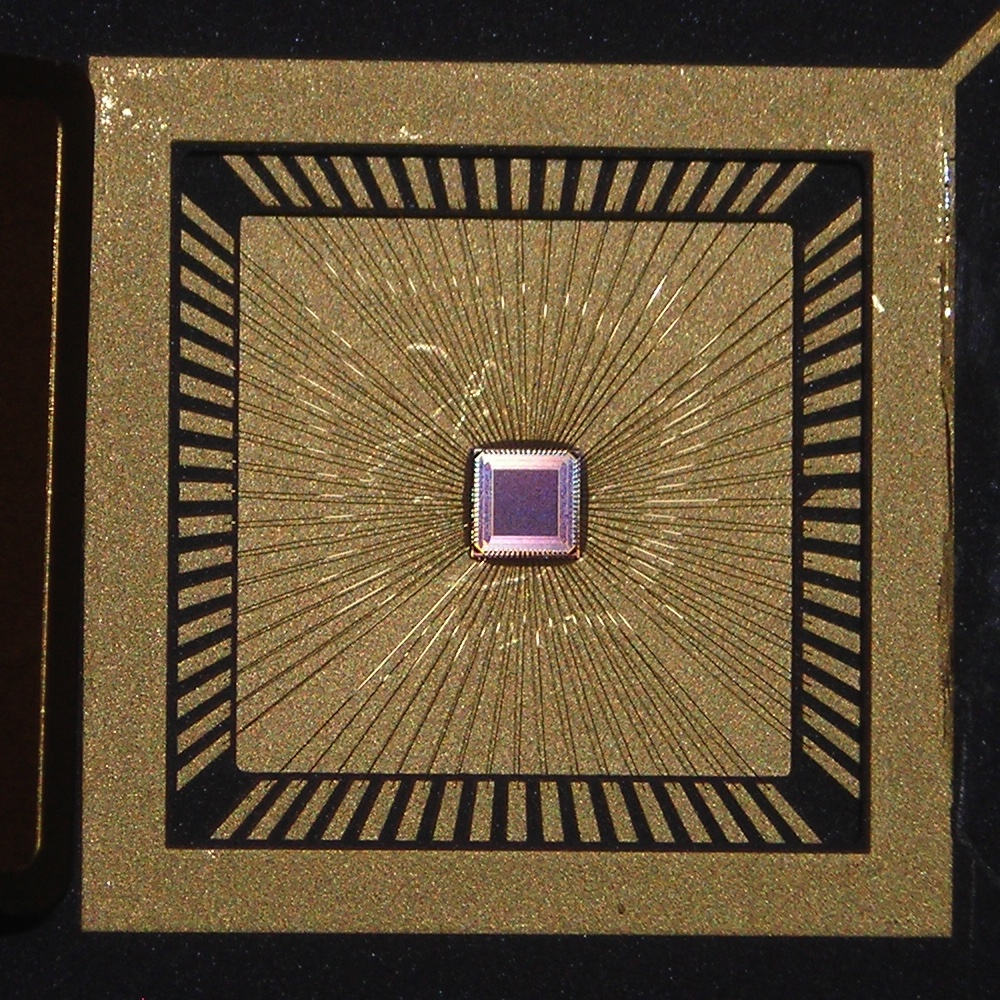
\includegraphics[width=\linewidth]{VertexDetector/Chronopix/Chronopix_image}
    \caption{Photograph of the prototype 3 chip in its package. The chip has $48\times48$ pixels, each with a size of $25\times\unit[25]{\micron^2}$.}
    \label{fig:VertexDetector:ChronoPixel:image}
\end{minipage}\hfill
\begin{minipage}[t]{0.49\textwidth}
    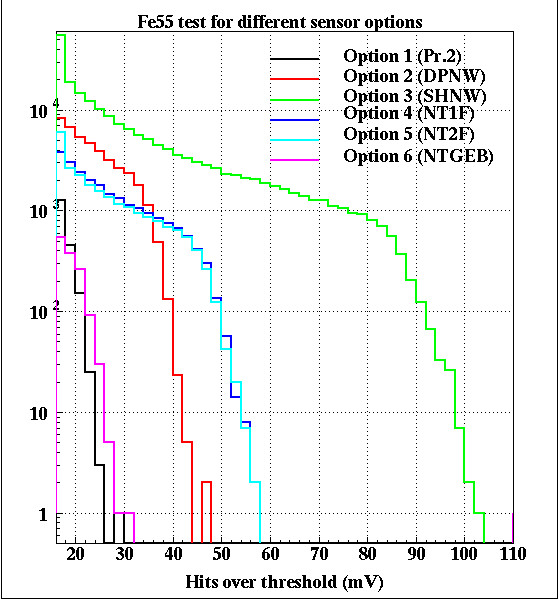
\includegraphics[width=\linewidth]{VertexDetector/Chronopix/Fe55tst}
    \caption{\ce{^{55}Fe} signal over threshold counts for 6 different sensor diode options,
implemented in prototype 3. For comparison, option 1 is the same as in prototype 2.}
    \label{fig:VertexDetector:ChronoPixel:Fe55Response}
\end{minipage}
\end{figure}
\begin{itemize}
    \item We have proven that we can record time stamps in every pixel with time resolution down to \unit[150]{ns}.
    \item We have tested sparse readout, allowing to read only pixels with hits, thus reducing readout time to the level allowing readout of all pixels in the sensor in the intervals between bunch crossings.
    \item We have tested pulsed power for the analog part of the pixels and have proven~\cite{sinev:Chronopix:FirstPrototype} that turning power ON about \unit[100]{$\mu$s} before bunch train and turning it off between bunch trains does not create any problems for threshold setting accuracy in the comparators.
    \item We have measured sensor noise level, including all pick-up and cross-talk. It was 24 e- r.m.s in prototype 1 and 26 e- r.m.s. in prototype 3, sensor option 3. Our specification was 25 e-.
noise.
    \item We have tested the idea of building all in-pixel electronics only from NMOS transistors, thus eliminating the need for a special process (deep p-well) to protect signal charge from parasitic collection by in-pixel transistors. We have proven~\cite{sinev:Chronopixel:RnDstatus2013} that all NMOS electronics can be built in this way, and that this does not significantly increase the power consumption compared to CMOS electronics.
    \item We have tested the compensation of comparator offsets using analog calibration, when the value of the offset is stored as a voltage on the capacitor in each pixel. This has an advantage over digital calibration (where the offset value is stored as code in the special register) in that there are no discrete levels, and the accuracy of such a calibration scheme is not affected by the size of the register or the spread of the initial offsets.
\end{itemize}
\subsection{Recent Milestones}
\begin{itemize}
    \item Test of prototype 2 revealed some problems. Possible solutions for these problems were discussed with Sarnoff engineers.
    \item A new contract with Sarnoff for the design of prototype 3 was signed in August 2013.
    \item Prototype 3 was manufactured in September 2014. Tests have shown that problems revealed in prototype 2 were solved.
\end{itemize}
The most recent report~\cite{sinev:POS:Vertex2105} on the status of ChronoPixel was presented by N.~Sinev in June 2015 at Vertex2015 in Santa Fe, New Mexico.

\subsection{Engineering Challenges}
\begin{itemize}
    \item The Vertex Detector for ILC faces many engineering challenges. The sensors need to be thinned to about \unit[50]{\micron} to reduce the amount of material in the detector. Support structures also need to be very light, but provide enough stability. Power dissipation of the entire detector should be small to be able to use only air cooling.
    \item If acceptable levels of the sensor diode capacitance can be achieved, the signal-to-noise ratio will improve. However, a lower value of the capacitance will make the pixels more sensitive to cross-talk through capacitive coupling. Reducing this coupling can be a challenge.
    \item Transition from small prototypes (few $\text{mm}^{2}$) to ILC detector size ($\approx \unit[10]{cm^2}$) may meet additional problems. One of them will be the effect of Lorentz forces on the power supply buses, especially in the case of power pulsing. Power pulsing is the only way to achieve acceptable power dissipation in the vertex detector. However, it will generate varying Lorentz forces, acting on power supply lines. This may produce vibrations, which are unacceptable for the required spatial resolution of the detector.
\end{itemize}

\subsection{Future Plans}
\begin{itemize}
    \item To achieve signal-to-noise ratio required for close to 100\% signal registration efficiency. We have achieved very low sensor capacitance in prototype 3, and the signal-to-noise ratio with such a sensor capacitance for \ce{^{55}Fe} signal is about 60, however, for minimum ionizing particles the signal will be much smaller, depending on epitaxial layer thickness and charge collection efficiency. The signal-to-noise ratio for standard \unit[7]{\micron} epitaxial layer will be 20 if the charge collection efficiency is 100\%, which is unlikely (we have not measured it yet). So we probably will need to increase the epitaxial layer thickness.
    \item To achieve the required pixel size (prototype 3 has \unit[25]{\micron} pixels, we would eventually like \unit[15]{\micron}). It may require going to a technology with feature size less than \unit[65]{nm}. There seems to be no problems in that, but both -- good signal-to-noise ratio and pixel size requirements may be challenging.
    \item To achieve acceptable level of inter-pixel and digital-to-analog circuit cross talks and parasitic feedback.
    \item Depending on available funding, to build a complete sensor with a large enough area and full feature readout.
\end{itemize}

\subsection{Applications Outside of Linear Colliders}
     With some modifications (for example, adding time-time converter) ChronoPixel architecture can be applied for any experiment requiring time stamping of individual hits -- it may be HL-LHC, CLIC and so on.

\section{CMOS}
\subsection{Introduction}
CMOS Pixel Sensors (CPS) combine high granularity with low material
budget and allow integrating the full signal processing circuitry on
the sensor substrate. Being moreover cost effective because of the
underlying industrial market, CPS are attractive for a wide range of
applications. They are developed for the ILC since more than fifteen
years and were shown to rather easily comply with the required spatial
resolution and material budget of an ILC vertex detector and their
radiation tolerance was observed to go well beyond the ILC requirements~\cite{Behnke:2013lya}. The state of the art of the technology is illustrated
by the 400 ULTIMATE sensors  operated in the STAR-PXL detector~\cite{Greiner201168}
at RHIC/BNL since 2014 and by the 10-100 times faster
sensors developed for the upgrade of the ALICE Inner Tracker System
(ITS)~\cite{0954-3899-41-8-087002}.

The achieved read-out speed of the CPS developed for an ILC
vertex detector is already quite satisfactory~\cite{Behnke:2013lya},
but is worth
improving in ordre to facilitate track seeding at nominal ILC
running conditions and to introduce a safety margin reflecting the
uncertainties affecting the predicted beam related background rate.

The technology should in fact allow single bunch tagging, provided power
consumption and, in turn, power cycling remain under control. The flexibility and detection performances of CPS are also indicating attractive perspectives for trackers, where relaxed constraints on the granularity may be exploited
to find a well suited balance between speed, power saving and material budget. Ambitious goals for an ILC experiment may therefore be considered
since their development may be carried out for numerous years until the design
inputs of a vertex detector ought to be fixed.

The charged particle detection performances of CPS are
currently essentially limited by manufacturing parametres.
The latter evolve steadily since several years in a direction which makes
them increasingly suited to the ILC vertexing and tracking. Besides
achievements targetted with existing processes, the present R\&D
addresses also improvements expected from the evolution of the CMOS
industry, mainly driven by the trend towards smaller feature sizes which
would allow overcoming the conflict between the spatial resolution and the
bunch tagging capability of CPS. This evolution is already well visible
when comparing the performances achieved with the $\unit[0.35]{\mu m}$ process
used for the STAR-PXL and the more recently addressed $\unit[0.18]{\mu m}$ process
used for the ALICE experiment.


The R\&D adresses presently four objectives :
\begin{itemize}
\item 2 or 3 CPS variants optimised for the different vertex detector layers :
\begin{itemize}
\item inner layer : design privileging spatial resolution and read-out speed
\item outer layers : design privileging power saving, exploiting the
				less demanding spatial and time resolutions
\end{itemize}
\item CPS adapted to tracking sub-systems, based on large pixels and privileging
power saving
\item ultra-light double sided ladders (called PLUME~\cite{Nomerotski2011208})
equipped with (identical or complementary) CPS on its two faces
\end{itemize}


\subsection{Recent Milestones}
Specific CPS are being developed since 2011 to equip the Inner Tracking
System (ITS) of the ALICE experiment in the framework of its upcoming
upgrade. The surface to cover exceeds 10 square meters, i.e. nearly two
ordres of magnitude more than the STAR-PXL or an ILC vertex detector.

Two CPS are being developed, differing by their read-out architectures.
The most conservative of them, called MISTRAL-0, reproduces the ULTIMATE
sensor equipping the STAR-PXL and is thus based on a synchronous, rolling-shutter, read-out. The concept underlying the other sensor, called ALPIDE, features an asynchronous read-out based on a token ring relying on a pre-amplifier/shaper/discriminator chain implemented in the pixel array. It
allows for a few microsecond read-out time and for a power consumption below
$\unit[50]{mW/cm^2}$. These performances were demonstrated in 2014~\cite{1748-0221-10-03-C03030}
on a real scale prototype.

MISTRAL-O relies on large pixels to achieve a $\unit[20]{\mu s}$ read-out
time and a power consumption below $\unit[100]{mW/cm^2}$ while providing
$\unit[10]{\mu m}$ resolution with its integrated binary encoding.
Its read-out architecture was validated in 2014 with a real scale
prototype~\cite{Winter:NSSMIC:2014} featuring 160,000 small ($22\times\unit[33]{\mu m^2}$
large) pixels. More recently \cite{Winter:ALCW15}, prototypes composed of
three times larger pixels were tested on beam and demonstrated satisfactory
charged particle detection performances at
30\textdegree C and after radiation loads exceeding those expected at the
ILC by several ordres of magnitude.

In summary, the full chain of the ULTIMATE sensor has been reproduced
in a $\unit[0.18]\{mu m}$ process with twice faster read-out frequency and
improved sensitive volume (epitaxial layer) characteristics. The
optimisation of this design for tracking systems, using relatively
large pixels, is validated.

Moreover, a small prototype of a sensor optimised for the vertex detector
outer layers was realised in the $\unit[0.18]{\mu m}$ process mentioned earlier.
Low power is achieved using enlarged, $\unit[35]{\mu m}$ pitch, square pixels and the
spatial resolution is kept below $\unit[4]{\mu m}$ by integrating a 3-bit ADC in
each pixel. The approach was validated in the former $\unit[0.35]{\mu m}$ process
with the MIMOSA-31 prototype, but the ADCs had to be kept at the sensor
periphery because of process limitations, translating into larger
power consumption and slower read-out. Laboratory tests of the new
prototype were performed since last Summer, showing satisfactory noise performances at nominal read-out speed, thus validating the concept.


\subsection{Engineering Challenges}
Squeezing the material budget of the double-sided PLUME ladders
below $\unit[0.3\%]{X_0}$ will the main engineering challenge, as the design
has to account for the necessity to power pulse the ladders in the
strong experimental magnetic field. Power pulsing seems mandatory
in case of continuous read-out as the sensor design is unlikely to
end up with a power density suppressed enough to avoid switching
the sensors off inbetween consecutive trains. The possibility to
introduce micro-channel cooling in the ladders will be studied in
ordre to mitigate the power pulsing requirements.

\subsection{Future Plans}

Several development directions will be pursued in the coming years,
to improve the performances of the CPS and to assess the added value
of the ultra-light double-sided ladder concept.

The development of CPS will mainly aim at realising a prototype of
a new sensor series, called IBISCUS\footnote{standing for {\bf I}lc
{\bf B}unch {\bf I}dentifying {\bf S}ensor {\bf C}ompatible with
{\bf U}ltraprecise {\bf S}patial resolution},
composed of pixels with less than $\unit[20]{\mu m}$ pitch providing a
read-out time of about $\unit[1]{\mu s}$ (using a token ring read-out).

The R\&D on the other CPS versions mentioned earlier (for the vertex
detector outer layers and for tracking sub-systems) will be pursued
with coarser priority.
Besides these continuous read-out architectures, a sensor composed
of $\unit[4]{\mu m}$ pitch square pixels with analog output, foreseen to be
read out inbetween trains like FPCCDs, will also be studied.

% Studies have shown \cite{1748-0221-10-03-C03030} that the track reconstruction
% would still improve if the sensors could separate individual bunch
% crossings, thus

Different versions of double-sided ladders will be realised and
their performances evaluated in terms of spatial accuracy, including
alignment issues, and in terms of stability against power pulsing,
possibly in a high magnetic field.

The two main alternative design options are going to be compared
to each other. One version is based on a high precision sensor
($<\unit[3]{\mu m}$) on one side featuring $\lesssim\unit[50]{\mu s}$ integration
time, while a fast sensor ($\sim\unit[2-3]{\mu s}$) equips the other side
which provides $\sim\unit[5]{\mu m}$ resolution. The other version is based
on a single sensor equipping both ladder sides, which offers $\sim\unit[4]{\mu m}$
spatial resolution and about $\unit[5]{\mu s}$ time resolution.

\subsection{Applications Outside of Linear Colliders}
CPS developed at IPHC in perspective of the ILC are used in several
devices, as illustrated by the non-exhaustive list below:
\begin{itemize}
\item Several high precision transparent beam telescopes, adapted to
	($<\unit[1]{GeV}$) electron beams, are equipped with the MIMOSA-26 or
	-28 (alias ULTIMATE) sensors
\item The first generation of sensors with full on-chip signal processing
	developed at IPHC (in a $\unit[0.35]{\mu m}$ CMOS process) was applied to the
	STAR-PXL detector at RHIC, which completed successfully its first
	data campaign in 2014 and has started its 2015 run
\item The upgraded ALICE ITS will be the next equipment based on CPS;
	it will provide insight of a token ring architecture pioneering
	the one considered for the IBISCUS chip mentioned above; it will
	also provide running experience with a tracker based on CPS
\item The Micro-Vertex Detector of the CBM experiment at FAIR/GSI will
	also be based on the CPS presently developed for the ALICE-ITS
	upgrade
\item The sensors were, or are, being applied outside of subatomic physics.
	They were for instance used in the FIRST experiment at GSI, for
	hadrontherapy monitoring; they are presently developed for soft
	X-Ray imaging and brain-imaging.
\end{itemize}

Sensors featuring pixels about 5 times larger than those equipping the STAR-PXL were fabricated in 2014, with different pixel design optimisations. Such large pixels are more exposed to the effects of signal charge recombination. The purpose of the paper is, among others, to show that the charge particle detection efficiency is not degraded, even after radiation loads representative of upcoming trackers, such the upgraded ALICE Inner Tracking System. The charged particle detection performances of these large pixel CPS prototypes with integrated signal processing and binary outputs were studied by exposing the sensors to a 450 MeV electron beam. The results obtained will be exposed
and shown to validate the concept for its evolution towards large area tracking devices, with the perspective of integrating logical strips in the sensor.

\section{DEPFET Pixel Sensors}

\subsection{The DEPFET Collaboration}
\href{http://www.hll.mpg.de/twiki/bin/view/DEPFET/CollaborationList}{The DEPFET collaboration} consists of nearly 100 members from 13 institutes. It currently takes responsibility for the following work packages:
\begin{description}
\item[Mechanics] {The DEPFET ladder integrates the support structure with the sensor wafer using state-of-the-art silicon processing technology. Read-out electronics and signal routing are integrated on the silicon wafer. The resulting all-silicon ladder is fully self-supporting. The mechanical properties of thin ladders in a realistic environment are studied in detail using detailed models (mock-ups) for Belle II and the ILC .}
\item[Cooling] {The DEPFET cooling concept for Belle II relies on two-phase \ce{CO2} cooling for the end-of-ladder. The sensor is cooled moreover with a forced flow of cold gas. The \ce{CO2} cooling plant is developed by KEK, while the design for the cooling block/support structure is performed within the collaboration. The impact of the linear collider cooling strategy - based on reducing the power dissipated using a pulsed power supply to the detector and cooling through a forced air flow - is studied. A novel cooling strategy for future applications based on mico-channels in the sensors is being evaluated in the collaboration. Solutions for monitoring of environmental parameters are being developed.}
\item[Ancillary ASICs] {The operation of a DEPFET detector requires ancillary electronics in the form of a read-out ASIC (the Drain Current Digitizer), a steering ASIC (SWITCHER) and on-detector ASICs for digital data processing (DHP). These ASICs are developed within the collaboration.}
\item[Data Acquisition and Trigger] {The development of off-detector electronics to process the data from the Belle II vertex detector.}
\item[Characterization of prototypes, laboratory and beam tests] {This work package has contributions from nearly all institutes involved in the DEPFET collaboration.}
\end{description}

Currently, the construction of the Belle II vertex detector~\cite{Abe:2010gxa} is the main focus of the collaboration. The requirements of the Belle II vertex detector are similar to those of the ILC, and more stringent in some aspects. The Belle II construction project therefore has considerable synergy with developments for a future linear collider. The LC-specific effort is focused on the development of small-pixel devices and the design of a forward vertex detector. We envisage that after the installation of the Belle II detector (2016) the balance between both projects is restored.



\subsection{Introduction}
The DEPFET technology implements amplification within the active pixel by integrating a p-MOS transistor in each pixel on the fully depleted high-resistivity silicon wafer. Additional n-implants near the transistor act as a trap for charge carriers created in the substrate (internal gate), so that they are collected beneath the transistor gate. The amplified signal is extracted from the pixel matrix by a numbers of ASICs~\cite{Kishishita:2014maa,Krueger2010337} mounted directly on the sensor: The SWITCHER, Drain Current Digitizer (DCD)~\cite{1748-0221-6-01-C01085,5446501} and Data Handling Processor (DHP)~\cite{1748-0221-7-01-C01069}. 



The DEPFET in-pixel amplification allows for a comfortable signal-to-noise ratio with a very thin active detector. The reduced sensor thickness of 75 $\micron$ for Belle II, 50 $\micron$ for the Linear Collider, is the key to remain within the material budget of 0.15\% of a radiation length per layer. DEPFET prototypes with 20$\times$ 20 $\micron^2$, small enough to meet the stringent spatial resolution specifications of the ILC, have successfully been operated in beam tests~\cite{Andricek:2011zza,Velthuis:2008zza}. The DEPFET matrix is read out in rolling shutter mode at a rate of 100 ns/row. For the column depths relevant for the ILC and Belle II a frame rate of several tens of $\mu$s is achieved~\cite{6484214}. The expected performance of a DEPFET-based vertex detector meets the specifications drawn up by the ILD experiment. DEPFET is also considered as a back-up solution to the SiD concept, in case the single bunch crossing time stamping proves to be out of reach.



\begin{table}
\centering
\caption{Comparison of ILC and Belle II requirements of a vertex detector}
\label{tab:Vertex:DEPFET:ILCBelleComparison}
\begin{tabular}{ccc}
    & ILC & Belle II \\
    \hline
    occupancy & 0.13 hits/$\micron^2$/s & 0.4 hits/$\micron^2$/s \\
    radiation & $< \unit[100]{krad/yr}$ & $> \unit[1]{Mrad/yr}$  \\
    & $\unit[10^{11}]{MeV n_{eq}/yr}$ & $2\times \unit[10^{12}]{MeV n_{eq}/yr}$ \\
    duty cycle & 1/200 & 1 \\
    frame time & $25-\unit[100]{\upmu s} $ & $\unit[20]{\upmu s}$ \\
    momentum range & 100 keV - 500 GeV & $ < \sim\unit[1]{GeV}$ \\
    angular acceptance & 6\degree - 174\degree & 17\degree - 150\degree \\
    spatial resolution & excellent: $3-\unit[5]{\micron}$ & moderate \\
    pixel size & $20\times \unit[20]{\micron}$ & $50\times \unit[75]{\micron}$ \\
    material budget & 0.15\% $X_0$/layer & 0.21\% $X_0$/layer \\
\end{tabular}
\end{table}

\subsection{Recent Milestones}
The concept of a DEPFET active pixel detector for vertex detection at collider experiments was initiated in the linear collider community (for TESLA).
The operation principle was extensively proven~\cite{Andricek:2011zza,Velthuis:2008zza} on small-scale prototypes. A recent reassessment of the DEPFET potential for a linear collider at the energy frontier is found in~\cite{6484214} and in the report~\cite{depfet_ecfa_report} for the ECFA detector R\&D review in 2014.
A large-scale, \unit[75]{\micron} thin Belle II ladder with the ancillary ASICs integrated on the sensor was successfully submitted to a test in an electron beam at DESY in January 2014\cite{Marinas:2014iza}.


The first full-scale DHP prototype was implemented in IBM \unit[90]{nm} CMOS technology. As this technology was discontinued, more recent designs were submitted in the TSMC \unit[65]{nm} CMOS process. DHPT v.1.0 comprises temperature independent current references, 11 bias 8-bit DACs with current output, an integrated temperature measuring system and JTAG control. This design has been successfully tested during early 2014\cite{Kishishita:2014maa}.

\subsection{Engineering Challenges}
Vertex detector ladders with a thickness of several tens of microns and a spatial resolution of well below \unit[10]{\micron} require very robust mechanical properties. The power generated by the sensors and ASICs must be removed with the smallest impact on the detector material.
Measurements on thin ladders under a realistic load, including pulsed powering according to the ILC beam structure, prove the excellent mechanical properties of the all-silicon ladder~\cite{thermomech}.

\subsection{Future Plans}
Currently, the construction of the Belle II vertex detector (to be installed by 2016 for the first physics run in 2017) implies a large effort of R\&D, including:
\begin{itemize}
\item Develop the die-attach technology in a controlled atmosphere required for the mounting of passive components on the DEPFET active pixel detector ladders. The first milestone is a fully integrated electrical prototype based on the EMCM.
\item First tests that will determine if all the ASICs on the ladder are fully functional
\item The integration of read-out and steering ASICs on the pixel sensor to be performed using a flip-chip technique and so-called bump-bonding, using microscopic solder balls.
\item The production of the Belle II vertex detector modules, a joint effort of the DEPFET collaboration
\item The test of the last version of the DHP chips
\end{itemize}
In the near future we hope to characterize the performance of a thin ILC-design prototypes with pixels of $20 \times \unit[20]{\micron^2}$
\begin{itemize}
\item Perform an engineering design for a DEPFET all-silicon module with the required petal geometry
\item A detailed characterization of the response of the device
\item Design of the ancillary ASICs, taking full responsibility for future design cycles of the Front End read-out chip, the Drain Current Digitizer (DCD) that is relevant to the ILC and a Belle II upgrade. This chip converts the analog signal from the detector to digital and has a crucial impact on the detector performance.
\end{itemize}

In the longer term the DCD and DHP are envisaged to evolve into a single chip. Being large arrays of DEPFET pixels a promising technology for the vertex detector of the planned ILC, adaptation of the DCD and DHP chips must also be done.

 In the near future we hope to characterize the performance of ILC design prototypes with pixels of $20 \times \unit[20]{\micron^2}$.
Important experience is furthermore gained with the thermal and mechanical properties of ultra-thin ladders. Measurents on thin ladders under a realistic load, including pulsed powering according to the ILC beam structure, prove the excellent mechanical properties of the all-silicon ladder. A complete mock-up for the innermost disks is under construction.

\subsection{Applications Outside of Linear Colliders}
The concept of a DEPFET active pixel detector for vertex detection at collider experiments was initiated in the linear collider community (for TESLA). The election of DEPFET technology for the Belle II detector therefore represents an important spin-off of linear collider detector R\&D. DEPFET is also considered a strong candidate technology for the vertex detector at a future circular collider (http://cepc.ihep.ac.cn/preCDR/volume.html). DEPFET detectors are furthermore used for X-ray imaging at the XFEL~\cite{xfel}. Future space missions envisage the use of DEPFET sensors~\cite{bepicolombo}. Their use in microscopy is being studied.





\section{FPCCD}
\subsection{Collaborating Institutions}
\subsection{Introduction}
    Fine pixel CCD (FPCCD) is one of the candidate sensor options for the vertex detector of the ILD detector at the ILC~\cite{Sugimoto:2005ru,2009arXiv0902.2067S,2012arXiv1202.5832S}. In the present design, FPCCD sensors for the innermost layer of the vertex detector have a pixel size of \unit[5]{\micron} and a fully depleted epitaxial layer with a thickness of \unit[15]{\micron}. Because of the small size of the pixels, the occupancy is acceptably low even if the hits are accumulated for one nominal ILC bunch train ($\approx\unit[1]{ms}$).
    The efforts of the FPCCD collaboration are currently focused on pixel characterization and development, while we also pursue developments to the cooling system, electronics downstream of ASICs and the reconstruction software~\cite{Mori:2014xta}.
\subsection{Recent Milestones}
R\&D activity for the FPCCD vertex detector at present is mainly focused on FPCCD sensors and a detector cooling system using 2-phase \ce{CO2}.
One of the achievements of FPCCD sensors after DBD is the fabrication of real size ($12.3 \times \unit[62.4]{\mathrm{mm}^2}$) sensors with \unit[50]{\micron} total thickness. Figure~\ref{fig:FPCCD:realSizeSensor} shows the real size prototype sensor. It has 8 readout nodes, and each channel has different pixel sizes of \unit[12]{\micron}, \unit[8]{\micron}, and \unit[6]{\micron}.
\begin{figure}
 \begin{minipage}[t]{0.49\textwidth}
\centering     \includegraphics*[width=\textwidth,keepaspectratio]{VertexDetector/FPCCD/realSizeFPCCDSensor.png}
    \caption{Real size FPCCD sensor thinned down to \unit[50]{\micron}}
    \label{fig:FPCCD:realSizeSensor}
 \end{minipage}
 \hfill
 \begin{minipage}[t]{0.49\textwidth}
 \centering
    \includegraphics*[width=\textwidth,keepaspectratio]{VertexDetector/FPCCD/coolingSystemSchematic.png}
    \caption{A simplified schematic diagram of the two-phase $\text{CO}_2$ cooling system}
    \label{fig:FPCCD:coolingSystemSchematic}
 \end{minipage}
 \end{figure}

We have started a neutron damage test using small ($\unit[6]{mm}\times\unit[6]{mm}$) FPCCD prototypes~\cite{lcws:fpccd:ito:2013}. A prototype sensor was irradiated by a neutron beam of few tens of MeV at the CYRIC facility of Tohoku University. The detailed analysis on the irradiated sensor is still on-going.
In order to increase the radiation immunity of FPCCD sensors, particularly to reduce the transfer inefficiency due to radiation damage, the sensors should be cooled down to \unit[-40]{\degree C}. We have started R\&D on a two-phase \ce{CO2} cooling system for this purpose. There are several examples of utilizing two-phase \ce{CO2} cooling systems for high energy physics experiments. For these cases, the \ce{CO2} coolant is circulated using liquid pumps. This method is, however, not so efficient for very low temperature cooling of \unit[-40]{\degree C}. Therefore, we adopted a \ce{CO2} gas compressor for the circulation of \ce{CO2} coolant. Figure~\ref{fig:FPCCD:coolingSystemSchematic} shows a simplified schematic diagram of the system. A prototype system has been constructed, and cooling between \unit[-40]{\degree C} and \unit[+15]{\degree C} has been successfully demonstrated using this system.

\subsection{Engineering Challenges}
    In the present design of the ILD vertex detector, two sensor layers are mounted on both sides of a light-weight ladder of ~\unit[2]{mm} thickness. Our goal of the material budget of this ladder is 0.3\% X0/ladder = 0.15\% X0/layer. This goal would not be so easy to accomplish, and we need a lot of R\&D effort.
    The ladders have to be cooled down to \unit[-40]{\degree C}. We plan to achieve this cooling by heat conduction to the end-plate on which thin cooling tubes for 2-phase \ce{CO2} are attached. The design of this structure is not trivial, and we need R\&D including thermal simulation.
    There are challenges both with the mechanical structure and the electronics circuit for the ladder R\&D. We have not started this effort yet.
\subsection{Future Plans}
    We have been doing our R\&D on the FPCCD vertex detector based on a Grant-in-aid for science research which expires at the end of FY2015. By that time, we plan to carry out the following R\&D items:
\begin{itemize}
    \item Characterization of FPCCD sensors including beam tests and radiation damage tests
    \item Development of FPCCD sensors with the pixel size of \unit[5]{\micron}, which is our ultimate goal
    \item Construction of prototype ladders for inner layers
    \item Development of readout electronics downstream of ASICs
\end{itemize}
If new funding is secured in future, the following R\&D items have to be done:
\begin{itemize}
    \item Development of larger FPCCD sensors and prototype ladders for outer layers
    \item Development of readout electronics which can fit in the small space of real experiment
    \item Construction of a real size engineering prototype and its cooling test
\end{itemize}

\subsection{Applications Outside of Linear Colliders}
    Because of the relatively slow readout speed, the application of FPCCD sensors to other high energy physics experiments would be limited. However, high spatial resolution of small pixel size must be applicable to measurements of X-ray imaging.
    Two-phase \ce{CO2} cooling system can be applied to any other detectors which require efficient cooling between \unit[-40]{\degree C} and near room temperature. Our system, which uses a \ce{CO2} gas compressor, has a great advantage for low temperature operation near \unit[-40]{\degree C} compared with systems using liquid pumps for circulation.

\section{SOI}
Contact person: Yasuo Arai (email: yasuo.arai@kek.jp)
\subsection{Introduction}
\subsection{Recent Milestones}
At present, major issues in the SOI pixel development are ``back-gate effect'', ``hole trap under the transistors by radiation,'' and ``sensor-circuit cross talks'' as shown in Figure~\ref{fig:VertexDetector:SOI:SOI_Schematic}. For these, we have been developing a double SOI technology. The developed double SOI wafer has an additional middle-SOI(Si) layer under the transistors. The conduction layer of the middle-SOI can solve all the three issues. We could successfully process the double-SOI wafer (Figure~\ref{fig:VertexDetector:SOI:crossSectionAfterProcessing}). Threshold shift by radiations is successfully recovered by applying compensating voltage to the middle SOI layer (Figure~\ref{fig:VertexDetector:SOI:thresholdShift}).

\begin{figure}
 \begin{minipage}[t]{0.49\textwidth}
\centering     \includegraphics*[width=\textwidth,keepaspectratio]{VertexDetector/SOI/SOI_Schematic}
\caption{Major issues in the SOI pixel detector and introduction of a middle-SOI layer}
\label{fig:VertexDetector:SOI:SOI_Schematic}
 \end{minipage}
 \hfill
 \begin{minipage}[t]{0.49\textwidth}
 \centering
    \includegraphics*[width=\textwidth,keepaspectratio]{VertexDetector/SOI/crossSectionAfterProcessing}
	\caption{Cross section of the double SOI chip after processing}
	\label{fig:VertexDetector:SOI:crossSectionAfterProcessing}
 \end{minipage}
 \end{figure}

\begin{figure}
\centering
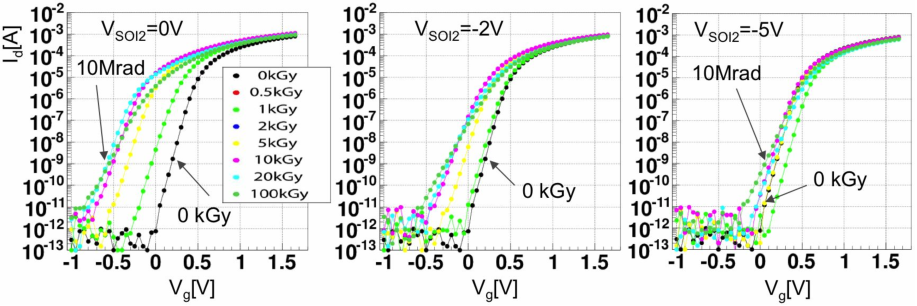
\includegraphics[width=\textwidth]{VertexDetector/SOI/thresholdShift}
\caption{Threshold shift recovery by applying compensating voltage (Vsoi2) to the middle Si layer}
\label{fig:VertexDetector:SOI:thresholdShift}
\end{figure}

\subsection{Engineering Challenges}
The impact parameter resolution for the ILC vertex detector is required to be a few \micron. This means the pixel size must be less than about \unit[20]{$\micron^2$}. On the other hand, each pixel must register arrival time of the hits during bunch train, which requires many transistors and capacitors to be located in each pixel.
A solution to this is 3D vertical integration of the circuit layers. SOI technology is ideally suited for 3D integration, since the thinning is stopped at the buried oxide (BOX). We already tried 3D SOI pixel chip in collaboration with T-Micro Co. Ltd. The process flow of micro-bump 3D connection is shown in Figure~\ref{fig:VertexDetector:SOI:microbump3D}. This process achieves a resistance of ($\sim$\unit[6]{$\Omega$}/bump) between upper and lower tiers for 1,000 daisy chain (2,000 bumps) as shown in Figure~\ref{fig:VertexDetector:SOI:resistanceOfDaisyChain}.
However, to achieve the density of digital circuitry necessary for ILC operations, \unit[32]{nm} technology may be necessary for the upper tier in the ILC. This requires bonding of two different technology wafers. The 3D integration of different technology wafers (or chips) is still an engineering challenge.

\begin{figure}
 \begin{minipage}[t]{0.35\textwidth}
\centering     \includegraphics*[width=\textwidth,keepaspectratio]{VertexDetector/SOI/microBump3DIntegration}
\caption{Micro-bump 3D integration process flow of the SOI pixel}
\label{fig:VertexDetector:SOI:microbump3D}
 \end{minipage}
 \hfill
 \begin{minipage}[t]{0.64\textwidth}
 \centering
    \includegraphics*[width=\textwidth,keepaspectratio]{VertexDetector/SOI/resistanceOfDaisyChain}
	\caption{Resistance of micro-bump daisy chain between upper and lower tiers}
	\label{fig:VertexDetector:SOI:resistanceOfDaisyChain}
 \end{minipage}
 \end{figure}

\subsection{Future Plans}
Detector R\&D plans for the coming years;
We are planning following items for the coming year.
\begin{itemize}
\item Sep. 2014 : Complete architecture study for the ILC pixel detector.
\item Mar. 2015 : Design and fabrication of first test chip for the ILC.
\item Dec. 2015 : Beam test of the test chip.
\end{itemize}

\section{3D Pixel Development}
\subsection{Collaborating Institutions}
\begin{itemize}
\item Brown University
\item Cornell University
\item Fermilab
\item Northern Illinois University
\item SLAC
\item University of Illinois Chicago
\end{itemize}
\subsection{Introduction}
This R\&D area covers sensors and electronics integrated utilizing 3-dimensional electronics technology.  This technology is distinct from 3D sensors and builds on efforts in the electronics industry to stack multiple layers of electronics to form dense assemblies of complex devices.  It is important for Particle Physics in that it allows very fine pitch (\unit[4]{\micron}) integration of sensors with multiple layers of electronics, allows interconnection to both the top and bottom of devices, and provides techniques for low mass, thinned devices. The interconnection of top and bottom means that sensors can be bonded to complex electronics with no wasted area for interconnect and optimal delivery of power and ground.
\subsection{Recent Milestones}
Major R\&D efforts and recent developments since ILC DBD (with publications/references to major results)
We have completed our multi-year effort to demonstrate commercial 3D technology. This consists of two tiers of \unit[0.13]{\micron} CMOS interconnected with Direct Oxide Bonding (DBI) technology and access using Through-Silicon-Vias (TSV). The DBI bonds are at \unit[4]{\micron} pitch. Fermilab sponsored the first 3D multiproject run for Particle Physics. The wafers were delivered last summer. Fermilab had three chips on the run VICTR -- a CMS track trigger chip, VIPIC -- an X-ray imaging chip, and VIP -- an ILC vertex chip. Test of the VIPIC and VICTR have shown working devices.  Tests for the VIP chip were delayed due to lack of funding and personnel.  We have recently restarted this work and initial tests are promising with the readout token successfully passed through the VIP.

In addition to the development of the 3D chips we have also explored the use of DBI to connect the 3D electronics with sensors.  Brookhaven Laboratory fabricated a sensor wafer with regions that mate to the VIP, VIPIC and VICTR chips.  The chips are ground to expose the top TSVs and contacts are deposited. The assembly is then attached to a handle wafer and the TSVs which project from the other side are exposed.  Wafers are then process for DBI bonding and individual die from the 3D wafer are bonded to the sensor wafer.  Finally the top ``handle'' silicon is ground and etched to reveal the previously formed contacts.  The total thickness of the readout at the end of this process is about \unit[25]{\micron} (Figure~\ref{fig:VertexDetector:VIP:chipsOnBNLWafer}). These wafers were received at the end of March 2014 and are being tested.
\begin{figure}
    \centering
    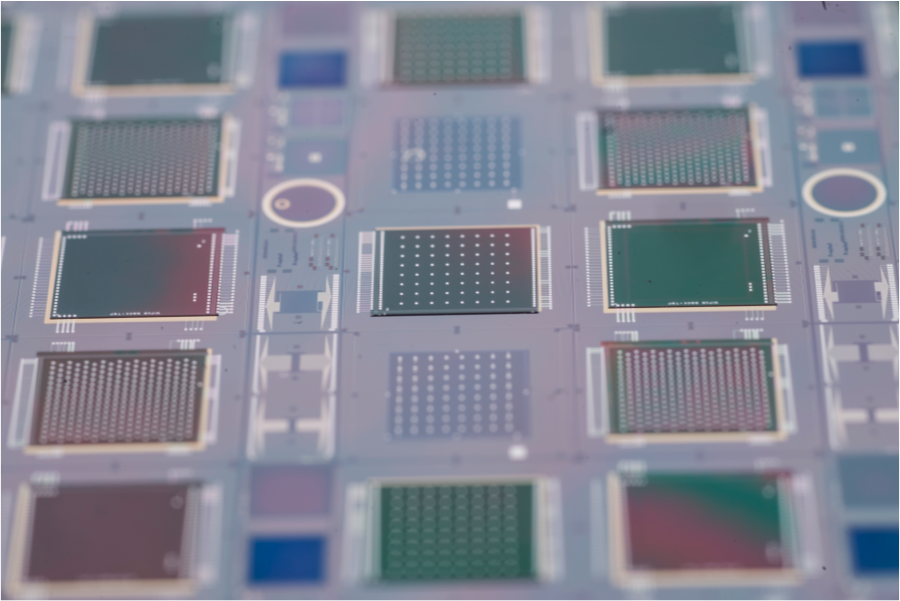
\includegraphics[width=.5\textwidth]{VertexDetector/VIP/3DChipsOnBNLWafers}
\caption{3D chips placed on BNL sensor wafers. VIP is middle left and right}
\label{fig:VertexDetector:VIP:chipsOnBNLWafer}
\end{figure}

Due to the fact that contacts to a 3D assembly can be made to the body of the die, rather than its edge space usually reserved for wirebond contacts at the edge can be eliminated.  This raises the possibility of fabricating large, complex pixel detectors of arrays of 4-side butted devices using sensors with active edges.  We are in the process of demonstrating this technology utilizing active edge sensors fabricated at VTT and using wafer-to-wafer bonding to a 3D readout wafer. The active edge wafers are based on a silicon-on-insulator stack and thus can be fabricated with essentially arbitrarily thin sensors, in this case \unit[200]{\micron}. Sensor and dummy readout wafers have been fabricated and a test wafer is being etched at SLAC. We expect to have DBI bonded assemblies this summer.

\subsection{Engineering Challenges}
Major  engineering challenges include:
\begin{itemize}
\item Development of widely commercially available 3D technologies.  Based partly on our development the silicon brokers CMP, CMC, and MOSIS now include 3D multiproject runs as part of their standard offerings.
\item Development of high yield 3D bonded chip-to-wafer devices.  This is the subject of our active edge project.
\item This development shares with other vertexing technologies the problems of low mass mechanical support, power delivery, and cooling. An SOI-based device can be made thin without special effort. Such thinned devics will need low mass backing hybrid circuitry, presumably flex on carbon fiber or a similar technology
\end{itemize}

\subsection{Future Plans}
\begin{itemize}
\item Complete the 3D active edge project
\item Apply our concepts to x-ray imaging devices
\item ILC developments would await renewed funding in the US.
\end{itemize}

\subsection{Applications outside of Linear Colliders}
As stated above the technology is already being developed for CMS and x-ray imaging applications.  The large area sensor concept is applicable for a variety of focal plane array concepts.

\begin{enumerate}
\item \bibentry{Deptuch:2013ona}
\item \bibentry{Yarema:2014mva}
\item \bibentry{MAJ:2013fwa}
\item \bibentry{2013arXiv1307.4301D}
\item \bibentry{1748-0221-7-12-C12010}
\item \bibentry{1748-0221-8-01-C01052}
\end{enumerate}

\section{CLICpix}
% \subsection{Collaborating Institutions}
% The vertex-detector R\&D for CLIC is carried out in the framework of the CLIC detector and physics
% collaboration (CLICdp), presently composed of 25 institutions~\cite{CLICdp-collaboration}.
% The main contributors to the vertex-detector
% project are
% Cambridge University,
% CERN,
% University of Geneva,
% Karlsruhe Institute of Technology (KIT),
% University of Liverpool,
% SLAC,
% Institute of Space Science Bucharest and the
% Spanish Network for Linear Colliders

\subsection{Introduction}
 The precision physics needs at the CLIC TeV-scale linear electron-positron collider
require a vertex-detector system with excellent flavour-tagging capabilities through
a measurement of displaced vertices in an environment with high rates
of beam-induced background events~\cite{Miyamoto:1425915}.
As a result, the CLIC vertex-detector system needs to have excellent spatial resolution
(\unit[3]{\micron}),
full geometrical coverage extending to low polar angles, extremely low material budget
(0.2\% $X_0$ per layer),
low occupancy facilitated by time-tagging (\unit[10]{ns} precision), and sufficient heat
removal from sensors and readout.
A concept based on hybrid pixel-detector technology is under development
for the CLIC vertex detector. It comprises fast, low-power and small-pitch readout
ASICs implemented in \unit[65]{nm} CMOS technology (CLICpix) coupled to ultra-thin planar sensors
or active HV-CMOS sensors via low-mass interconnects. The power dissipation of the
readout chips is reduced by means of power pulsing, allowing for a cooling system
based on forced gas flow. Through-Silicon Via (TSV) vertical interconnects remove the need for wire
bonding connections on the side of the readout ASICs
and therefore allow for an efficient tiling to form larger modules with minimal
inactive areas.
\subsection{Recent Milestones}
A broad hardware R\&D program is in place, addressing the challenges for the CLIC
vertex detector in an integrated approach~\cite{1748-0221-10-03-C03025}. Recent achievements
in the sensor and readout domain include:
\begin{description}
\item[Hybrid pixel assemblies with ultra-thin planar sensors]
Planar pixel sensors with \unit[55]{\micron} pitch and different thicknesses (\unit[50--300]{\micron})
were procured from different vendors and bump-bonded to Timepix~\cite{Llopart2007485} readout
ASICs (100 and \unit[700]{\micron} thickness).
Slim-edge sensor designs are compared to designs
with active edges.
Preliminary beam-test results show very good efficiencies in both cases, extending beyond the
edge pixels~\cite{Redford:1966932}.
For \unit[50]{\micron} sensor thickness and nominal readout parameters, the fraction of multi-pixel clusters
is approximately 20\%.
Single-point resolutions of approximately \unit[3]{\micron} have been extracted
for clusters of two pixels using charge interpolation and taking into account
non-linear charge sharing.
\item[CLICpix demonstrator ASIC]
A CLICpix demonstrator chip has been produced in \unit[65]{nm} CMOS technology,
including a $64 \times 64$ pixel matrix and power-pulsing capability~\cite{Valerio:1507691}.
The pixel size is $\unit[25]{\micron}\times\unit[25]{\micron}$. Simultaneous
4-bit Time-Of-Arrival (ToA) and Time-Over-Threshold (ToT) measurements
are implemented in each pixel, allowing for a front-end time slicing
with approximately \unit[10]{ns} and for measuring the charge
to improve the position resolution through interpolation.
The full chip can be read out in less than
$\unit[800]{\upmu s}$ (for 10\% occupancy), using a \unit[320]{MHz} readout clock and zero suppression.
The
power consumption of the chip is dominated by the analog frontend
with a peak power corresponding to $\unit[2]{W/cm^2}$. The total average power
consumption can be reduced to a value below the target of $\unit[50]{mW/cm^2}$
by means of power gating for the analog part and clock gating for the digital part.
Readout tests have confirmed that the CLICpix demonstrator chip
is fully functional and the power consumption and performance are in agreement with
simulations~\cite{clicpix-twepp-2013}.
Hybrid modules of CLICpix ASICs with planar slim-edge
sensor prototypes are currently in production.
\item[Capacitively coupled active HV-CMOS sensors]
Hybrid assemblies of CLICpix prototype chips with CCPDv3 active sensors
have been produced and tested.
The sensors are implemented in
a \unit[180]{nm} high-voltage CMOS process~\cite{Peric2013131}. A deep n-well above the low-resistivity
(few $\Omega$cm) p substrate
surrounds low-voltage p-wells and acts as the signal collecting electrode.
A nominal operation voltage of -\unit[60]{V} at the
n-well results in a depletion layer of approximately \unit[10--20]{\micron} in the p substrate.
 The fast drift signal collected in this
depletion layer passes through a two-stage transimpedance
amplifier in each pixel and the resulting voltage signal is capacitively coupled to the CLICpix
ASIC through a layer of glue a few microns thick.
Laboratory tests with radioactive sources show a good signal-to-noise performance for the
active sensor output. Preliminary test-beam results with CLICpix-CCPDv3 assemblies suggest a
detection efficiency of $>99\%$ for minimum ionising particles and a high fraction of
single-pixel clusters with a position resolution of
approximately \unit[7]{\micron}, as expected for \unit[25]{\micron} pixel pitch.
\item[Through Silicon Vias (TSV)]
A ``via last'' TSV process developed in collaboration with
CEA-LETI has demonstrated the feasibility of TSVs on functional
readout ASICs from the Medipix/Timepix chip family~\cite{6575630}.
The project uses Medipix3 readout wafers produced in \unit[130]{nm} CMOS
technology. The wafers are thinned to \unit[120]{\micron} and the resulting vias
have a diameter of \unit[60]{\micron}.
An ongoing  continuation of the TSV project aims at producing
TSVs in Timepix3 ASIC wafers thinned to \unit[50]{\micron}.
\end{description}
\subsection{Engineering Challenges}
The detector performance requirements lead to challenging constraints
for the mechanical and electrical integration of the vertex-detector
components and its cooling system. An integrated approach is followed,
addressing several of the critical R\&D issues in these domains:
\begin{itemize}
\item \emph{Power delivery and power pulsing.} A low-mass power-pulsing and power-delivery
system optimised for the small duty cycle of the CLIC machine has been
developed~\cite{fuentes-twepp2013}. Controlled current sources
deliver a low and almost constant current ($<\unit[300]{mA}$ per ladder)
into the vertex region through low-mass cables. The energy needed by the readout ASICs during the time of the collisions
and detector readout is stored locally in silicon capacitors. Low-dropout regulators provide the necessary stability
of the output voltage for the analog ($\Delta V\approx16$mV) and the digital part
($\Delta V\approx\unit[70]{mV}$) of the readout ASICs.
Prototypes have been tested successfully with dummy loads emulating the power consumption
of the 12 readout ASICs in a half ladder. The total contribution of the
powering infrastructure to the material budget of each barrel layer is
approximately 0.1\%X$_0$. It is expected to decrease to less than $0.05\%$X$_0$ with evolving silicon-capacitor technology.
\item \emph{Cooling.} Even with power pulsing a total power of approximately \unit[500]{W} will be dissipated in the vertex detectors alone. To limit the amount of material in the vertex-detector region, a cooling
system based on forced air flow is under development~\cite{DuarteRamos:1572989}. Finite-element Computational Fluid Dynamics (CFD) simulations show that air cooling is feasible. For a mass flow of \unit[20]{g/s}, the temperature increase
in the vertex detector is limited to approximately \unit[40]{\textdegree C}. The proposed cooling scheme is being
validated in thermal mockups. Preliminary results confirm the validity of the simulations.
\item \emph{Mechanical supports.} The low overall material budget leaves only about 0.05\%X$_0$ per
detection layer for mechanical supports. Prototypes based on Carbon-Fibre-Reinforced Polymers
(CFRP) are under study~\cite{VillarejoBermudez:1982810}. Bending-stiffness calculations have been validated in
finite-element simulations
and with bending tests. Measurements within an air-cooling mockup show
that the air-flow induced vibrations are at an acceptable level of approximately $\unit[1-2]{\micron}$ RMS
amplitude for the direction perpendicular to the detector plane and at nominal flow conditions.
\item \emph{Assembly and access scenarios.}
Assembly and access scenarios for in-situ testing have been developed,
taking into account the constraints from the surrounding detector elements~\cite{VillarejoBermudez:1982810}.
Realistic cabling layouts are proposed and evaluated in terms of their impact on the
global and local material budget.
\end{itemize}
\subsection{Future Plans}
The technical development programme for the CLIC vertex detector aims at building
demonstration modules for the main components of the vertex detector system
in time for the next update of the European Strategy
for Particle Physics in 2018/19. To reach this medium-term goal, several technology prototypes
are under development.
Ultra-thin edgeless hybrid pixel assemblies with Timepix3 readout ASICs (including ASICs thinned to \unit[50]{\micron}
and processed with TSVs) are currently in production.
The next version of the CLICpix demonstrator
ASIC (CLICpix2) is foreseen to be produced in the second half of 2015. It contains a larger
pixel matrix ($128\times 128$) and higher dynamic range (8-bit ToA and 5-bit ToT).
Slim-edge and edgeless sensors matching the $128\times 128$ CLICpix2 footprint have already been produced and an
improved version of the CCPD active HV-CMOS sensor will be submitted for production by the end of 2015.

\subsection{Applications Outside of Linear Colliders.}
The CLIC vertex-detector R\&D shares its main challenges of simultaneously achieving small pixel pitch,
low material budget and fast timing with other future pixel detector projects, such as the developments for
the upgrades of the LHC detectors for high-luminosity operation or for future circular colliders.
Synergies with these projects are exploited for example in the context of the RD53 collaboration for \unit[65]{nm} hybrid readout
ASICs~\cite{RD53} and via the AIDA2020 project for Advanced European Infrastructures for Detectors at
Accelerators~\cite{AIDA2020}.
Moreover the CLICpix ASIC is derived from the
Timepix/Medipix family of hybrid readout ASICs~\cite{medipix-collaboration}, which have a wide range of applications in
medical imaging and material science.

% \begin{sidewaystable}
% \begin{tabular}{|L{2cm}| L{4cm}| L{5cm}| L{7cm}| L{4cm}|}  \hline
%  \bf R\&D technology & \bf Participating Institutes &  \bf Description / Concept & \bf Milestones & \bf Future Activities \\ \hline
%  CLICpix &
% Cambridge University,
% CERN,
% University of Geneva,
% Karlsruhe Institute of Technology (KIT),
% University of Liverpool,
% SLAC,
% Institute of Space Science Bucharest,
% Spanish Network for Linear Colliders
%   &
%  Hybrid pixel-detector technology comprising fast, low-power and small-pitch readout
% ASICs implemented in 65 nm CMOS technology (CLICpix) coupled to ultra-thin planar
% or active HV-CMOS sensors via low-mass interconnects. &
% Beam tests of prototype assemblies with ultra-thin sensors (50-300 \micron);
% CLICpix demonstrator ASIC in 65~nm technology;
% Beam tests of assemblies with capacitive coupling between CCPDv3 HV-CMOS active sensors
% and CLICpix ASICs;
% Power-pulsing demonstrator with dummy loads;
% Prototypes of carbon-fibre ladder supports;
% Full-scale thermal mockup of the CLIC vertex-detector region.
% &
% Demonstration modules for all major components
% in time for the next update of the European Strategy
% for Particle Physics in 2018/19
%  \\  \hline
%   \end{tabular}
%
% \end{sidewaystable}

% % add references
% \begin{thebibliography}{99}
%
% \bibitem{CLICdp-collaboration}
% CLICdp collaboration, \href{http://clicdp.web.cern.ch}{http://clicdp.web.cern.ch}
%
% \bibitem{HVCMOS}  I. Peric et al.,
%   \emph{High-voltage pixel detectors in commercial CMOS technologies for ATLAS, CLIC and Mu3e experiments},
%  NIM~{\bf A731} (2013) 131, \href{http://dx.doi.org/10.1016/j.nima.2013.05.006}{10.1016/j.nima.2013.05.006}.
%
% \bibitem{RD53}
% RD53 collaboration, \href{http://rd53.web.cern.ch/}{http://rd53.web.cern.ch/}.
%
% \bibitem{AIDA2020}
% AIDA2020 Advanced European Infrastructures for Detectors at
% Accelerators, \href{http://aida2020.web.cern.ch/}{http://aida2020.web.cern.ch/}.
%
% \bibitem{medipix-collaboration}
% Medipix project, \href{https://medipix.web.cern.ch/medipix/index.php}{https://medipix.web.cern.ch/medipix/index.php}.
% %\printbibliography[title=References]
% \end{thebibliography}

\newpage
\thispagestyle{empty}
\newgeometry{margin=1.5cm} % modify this if you need even more space
\begin{landscape}
\begin{sidewaystable}
    \centering
    \begin{adjustbox}{max width=1.1\textwidth,totalheight=1\textheight}
\begin{tabularx}{2\textheight}{lXXXX}
    \toprule
    R\&D Technology & Participating Institutes & Description / Concept & Milestones & Future Activities \\
    \midrule
        ChronoPix &
        University of Oregon\newline Yale University\newline Sarnoff Corporation &
        ChronoPix is a monolithic CMOS pixelated sensor with the ability to record up to two time stamps per pixel during the bunch train. Hits are read out in the time between bunches. &
        April 2014: Device tests of prototype 2 inform the design of prototype 3 to be submitted to foundry &
        Prototype 3 was manufactured in September 2014. Tests have shown that problems revealed in prototype 2 were solved. \\
    \midrule
        CMOS MAPS &
        IPHC Strasbourg \newline DESY, Hamburg \newline University of Bristol \newline University of Frankfurt &
        The CMOS pixel sensor uses as a sensitive volume the $\unit[10-20]{\micron}$ thin high-resistivity epitaxial Si-layer deposited on low resistivity substrate of commercial CMOS processed chips. The generated charge is kept in a thin epi-layer atop the low resistivity silicon bulk by potential wells that develop at the boundary and reaches an n-well collection diode by thermal diffusion. &
        2016 : production of CPS for the ALICE-ITS upgrade\newline
        2018/19 : production of CPS for the micro-vertex detector of the CBM experiment at FAIR/GSI\newline
        2018/19 : validation of light double-sided ladder concept combining highly granular sensors on one side with timestamping sensors on the other side\newline
        $< 2020$ : validation of power pulsing of double-sdied ladders inside a high magnetic field\newline
        2022/23 : finalisation of the R\&D on various CPS adapted to the different layers of a very high performance vertex detector at the ILC &
        Until 2018-2019: Development and production of CPS for the ALICE-ITS and CBM-MVD \newline Development of various CPS optimised for the different layers of a vertex detector at the ILC, with emphasis on bunch tagging \newline Development of low material double-sided ladders \\
    \midrule
        DEPFET &
        University of Barcelona, Spain \newline
        University of Bonn, Germany \newline
        Heidelberg University, Germany \newline
        Giessen University, Germany \newline
        University of Göttingen \newline
        KIT Karlsruhe, Germany\newline
        IFJ PAN, Krakow, Poland \newline
        MPI Munich \newline
        MPG HLL Munich, Germany \newline
        Charles University, Prague, Czech Republic \newline
        IFIC, CSIC-UVEG, Valencia, Spain \newline
        DESY, Hamburg, Germany \newline
        IFCA, CSIC-UC, Santander, Spain &
        The DEPFET technology implements a single active element within the active pixel by integrating a p-MOS transistor in each pixel on the fully depleted, detector-grade bulk silicon. Additional n-implants near the transistor act as a trap for charge carriers created in the substrate (internal gate), so that they are collected beneath the transistor gate. &
        2014: Full-scale \unit[75]{\micron} thin Belle II ladder in beam test at DESY &
        Development of die-attach technology \newline
        Full-scale test of all ASICs on ladder \newline
        Integration of read-out and steering ASICs on pixel sensor using flip-chip technique and microscopic solder ball bump-bonding \newline
        Production of Belle II vertex detector modules\newline
        Tests of the last version of the DHP chips \newline
        Engineering design for all-silicon module with petal geometry required for ILC\newline
        Detailed characterization of device response \newline
        Design of ancillary ASICs, taking full responsibility for future design cycles of the FE read-out chip, called Drain Current Digitizer \\
    \midrule
        FPCCD &
        KEK \newline
        Shinshu University \newline
        Tohoku University \newline
        JAXA, Japan Aerospace Exploration Agency &
        Fine Pixel CCD sensors have pixel sizes of \unit[5]{\micron} and a fully depleted epitaxial layer with a thickness of \unit[15]{\micron} &
        Fabrication of real size ($\unit[12.3]{mm} \times \unit[62.4]{mm}$) sensors with \unit[50]{\micron} total thickness \newline
        Neutron irradiation of a small ($\unit[6]{mm} \times \unit[6]{mm}$) FPCCD sensor \newline
        Construction of a prototype cooling system and demonstration of cooling between $-40\degree C$ and $+15\degree C$ &
        Characterization of FPCCD sensors including beam tests and radiation damage studies \newline
        Development of FPCCD sensors with a pixel size of \unit[5]{\micron} \newline
        Construction of prototype ladders for the inner layers of a vertex detector \newline
        Development of readout electronics downstream of ASICs \newline
        Development of larger FPCCD sensors and prototype ladders for outer layers \newline
        Development of readout electronics with a small footprint \newline
        Construction of a real size engineering prototype and cooling test \\
    \midrule
        3D Pixels &
        Brown University \newline
        Cornell University \newline
        Fermilab \newline
        Northern Illinois University \newline
        SLAC \newline
        University of Illinois Chicago &
        3D technology allows very fine pitch (\unit[4]{\micron}) integration of sensors with multiple layers of electronics, allows interconnection oto both the top and bottom of devices, and provides techniques for low mass, thinned devices. &
        Completed multi-year effort to demonstrate commercial 3D technology, consisting of \unit[0.13]{\unit} CMOS interconnected with Direct Oxide bonding technology and access using TSV. \newline
        Received readout wafers with thickness of \unit[25]{\micron}, processed with TSV and DBI to connect to 3D electronics \newline
        Currently working on active edge demonstrator devices &
        Complete the 3D active edge project \newline
        Apply concepts to x-ray imaging devices \newline
        Re-start ILC developments pending renewed funding \\
    \midrule
        SOI &
        KEK\newline
        University of Tsukuba \newline
        Tohoku University \newline
        Osaka University &
        In the Silicon-On-Insulator (SOI) technology the sensing and processing functionalities are separated in different layers; the sensing is provided by a high-resistive substrate connected through an insulating layer with the processing layer. &
        &
        Sep 2014: Complete architecture study for the ILC pixel detector \newline
        Mar 2015: Design and fabrication of first test chip for the ILC \newline
        Dec 2015: Beam test of the chip \\
    \midrule
        CLICPix
        &
        Cambridge University\newline
        CERN\newline
        University of Geneva\newline
        Karlsruhe Institute of Technology (KIT)\newline
        University of Liverpool\newline
        SLAC\newline
        Institute of Space Science Bucharest\newline
        Spanish Network for Linear Colliders
        &
        Hybrid pixel-detector technology comprising fast, low-power and small-pitch readout.
        ASICs implemented in \unit[65]{nm} CMOS technology (CLICpix) coupled to ultra-thin planar
        or active HV-CMOS sensors via low-mass interconnects.
        &
        Beam tests of prototype assemblies with ultra-thin sensors (50--\unit[300]{ \micron})\newline
        CLICpix demonstrator ASIC in \unit[65]{nm} technology\newline
        Beam tests of assemblies with capacitive coupling between CCPDv3 HV-CMOS active sensors
        and CLICpix ASICs\newline
        Power-pulsing demonstrator with dummy loads\newline
        Prototypes of carbon-fibre ladder supports\newline
        Full-scale thermal mockup of the CLIC vertex-detector region
        &
        Demonstration modules for all major components
        in time for the next update of the European Strategy
        for Particle Physics in 2018/19
        \\
    \bottomrule
\end{tabularx}
\end{adjustbox}
\end{sidewaystable}
\end{landscape}
\restoregeometry

\subsubsection{The AHCAL in ILD and SiD}
The AHCAL prototype development follows the ILD detector design, and the performance studies, which guide the R\&D, are performed in the ILD concept. The detailed AHCAL simulation, as implemented in the ILD, has been shown to reproduce test beam results, and the components realized in prototypes are represented in the engineering model of ILD. There is close consultation between CALICE and the concepts on prioritizing the R\&D which is still needed on the way to a realistic technical proposal.

The AHCAL also constitutes an option for the hadronic calorimeter of the SiD concept. It is straightforward to transfer the technical and integration solutions developed in the ILD context to SiD, because the basic geometry and the routing of signals are very similar. However, the detailed integration of the AHCAL in the engineering model and in the simulation is not yet as advanced as for ILD. For example, the optimization of the cell size still needs to be done for the SiD case with its smaller detector radius and the more finely segmented ECAL. Steps are being taken on the software side, but the engineering support is sub-critical. There is regular exchange between CALICE and SiD on these issues, both the conceptual as well as on the technical level.

\newpage
\chapter{Silicon Trackers}
\subsection{SCIPP Tracking R\&D}
SCIPP has been involved in Linear Collider tracking R\&D for a number of years, and its work has led to the development of a refined understanding of several generic tracking issues with potential applications for Linear Collider detectors. These include the use of resistive strips and dual-end readout for the determination of the longitudinal coordinate of the charge deposition on narrow electrodes [1] and limitations on silicon microstrip ladder length for precision narrow-strip sensors [2]. These studies are in fact dependent only on the properties of the electrode that collects the signal and propagates it to the readout electronics, and thus are independent of the sensor technology that generates the signals. Thus, this work may have relevance to detection issues across a wide array of fields.
Ongoing tracking R\&D is focused on the further development of the Long Shaping-Time Front End (LSTFE) microstrip readout ASIC. This properties of this ASIC have been explicitly optimized for the readout of long ladders of silicon strip sensors that are motivated by the need for precise low-mass central tracking for a Linear Collider Detector. With a small and straightforward change to the shaping properties of the ASIC, it could be reoptimized for use for the short strips and high occupancy that would be expected for ILC forward-tracking applications.
Similar to most ILC-oriented readout designs, the LSTFE features a long shaping time optimized to reduce voltage-referenced readout noise, as appropriate for narrow-strip, long-ladder applications. Unique to the LSTFE design, however, is the use of time-over-threshold readout to estimate the analog pulse-height generated by through-going subatomic particles. A pule-development and readout simulation developed at SCIPP suggested that the intrinsic statistical fluctuations of the charge-deposition process in 300 µm of silicon obviate the need for a precise measurement of deposited charge. A simulation of the centroid-finding (position-resolution) uncertainty provided by time-over-threshold readout showed little degradation relative to that provided by an exact measurement of deposited charge.
On the other hand, there are several advantages offered by the use of time-over-threshold readout. It is very simple to implement within a digital back-end to the LSTFE’s analog front end (the implementation would be on the same chip as the front-end readout), requiring only a measurement of the number of clock counts that the given channel is over threshold, and then the assembly and transmission of a single data word containing the time of the upward transition, the time over threshold after the transition, and the channel number. This happens in real time and is driven immediately off the chip into the DAQ, eliminating the need for buffering and ADC conversion. In particular, there is no limit to the rate at which particles can be detected other than the return-to-baseline of the analog signal, and so the data-accumulation rate capability of the device is very high. In addition, for forward tracking, for which short strips are envisioned, the shaping time can be shortened significantly. This will further improve the rate capability of the LSTFE readout, making it an excellent choice for the high-occupancy forward region.
Figure 1 shows the measured fractional charge uncertainty for the LSTFE prototype ASIC; for depositions expected from minimum-ionizing particles (1-4 fC) the fractional charge measurement uncertainty is approximately 15\%, which is small compared to the intrinsic fluctuations that arise from the deposition process.
\begin{figure}
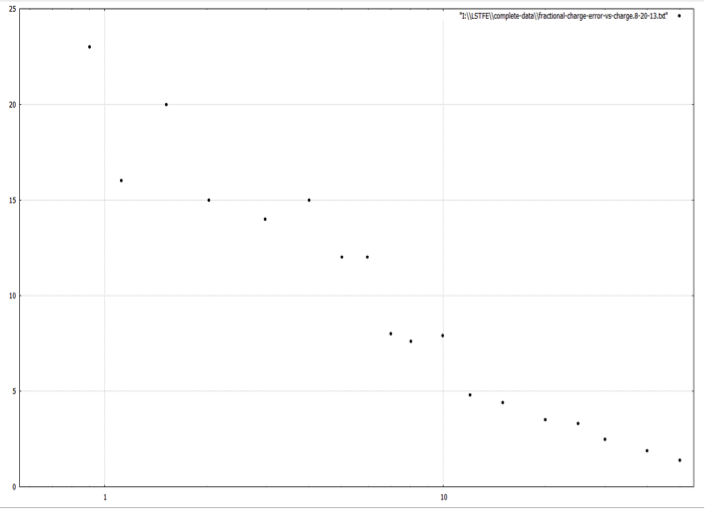
\includegraphics{Tracker/SCIPPTracking/SCIPPTracking}
\caption{Fractional pulse-height uncertainty (percent) versus injected charge (fC) for the LSTFE front-end ASIC.
The development of this ASIC has been done solely at the Santa Cruz Institute for Particle Physics (SCIPP) within the University of California at Santa Cruz, and while slowed significantly due to the loss of support for Linear Collider Detector R\&D, continues within SCIPP. Tasks that remain in developing a chip suitable for use in a Linear Collider Detector include the development of the digital back end; significant progress has already been made in defining the architecture of this section of the chip and in implementing this architecture in prototype form on an FPGA. Power cycling (switching the chip into a low-power quiescent mode for most of the 199 ms between beam crossings) also needs to be implemented.}
\end{figure}
 

References
[1] J. K. Carman et al., Longitudinal Resistive Charge Division in Multi-Channel Silicon Strip Sensors, Nulcear Inst. and Methods in Physics Research A579 (2007), pp 595-598.
[2] K. Collier et al., Microstrip Electrode Readout Noise for Load-Dominated Long Shaping-Time Systems, Nuclear Inst. and Methods in Physics Research, A729 (2013), pp. 127-132.

\section{Resistive charge-division on thinned micro-strips sensors with low signal amplification}
Contact person: Ivan Vila Alvarez (email: ivan.vila@csic.es)
\subsection{Introduction and Motivation}

In the context of the ILC, the relatively low occupancy environment and the power pulsing operation of the front-end electronics provide an opportunity for the implementation of ultra-lightweight silicon-based tracking systems where the dominant contribution to the material budget in the fiducial volume comes from the sensors. Reducing the material budget has a major impact on the hit position resolution and hence the momentum resolution of the tracker system; therefore, we have pursued during the last three years an RD program for the development of very thin micro-strips sensors able to provide two dimensional information of the hit position.

The ultimate goal of this R\&D is the development of a micro-strip sensor which combines signal amplification --- allowing the thinning of the sensor’s substrate --- and resistive electrodes --- allowing the implementation of the charge-division method for the determination of the hit position along the strip direction. In a first phase, we are aiming to demonstrate the feasibility of each of the above mentioned features independently and, in a second phase, to integrate both technological solutions into the same micro-strip sensor; the thinning of the sensor will done using the anisotropic wet etching (TMAH process) used for the DEPFET fabrication \ref{sec:DEPFET}.

\subsection{Recent Developments and Milestones}

The use of the charge-division method in long micro-strip sensors, with a length of several tens of centimeters, was proposed as a possible tracking technology for the International Linear Collider detector concepts a few years ago~\cite{Carman:2011zz}. More recently, we have demonstrated \cite{2012JInst...7.2005B,Bassignana2013186,Curras:ICHEP2014} the feasibility of the charge division concept on fully fledged micro-strip sensor with resistive electrodes made of poly-cristalline silicon achieving a spatial resolution along the strip direction of about 7\% the strip length. One of the limitations of this technology is the attenuation of the signal along the resistive electrode; additionally, the position resolution along the strip is proportional to the signal--to--noise ratio. Therefore, to maintain or even increase the SNR without increasing the sensor substrate thickness we proposed the integration of signal amplification structures in the sensor itself. The Low Gain Avalanche Detector (LGAD) technology appears as a well suited technique for achieving the signal amplification.
LGAD devices engineered as reach-trough avalanche detectors with a moderate gain where initially proposed and developed for timing application [Pellegrini 2014], the moderate signal amplification ensured that a relatively standard front-end readout electronics could be employed. As a spin-off of this original aim, we introduced the i-LGAD micro-strip concept for tracking, a LGAD device implemented in a p-type substrate where the ohmic electrode is strip-wise segmented; this design favors the uniform signal amplification over the sensors active volume overcoming the non-uniform gain in LGAD micro-strips sensors with a strip-wise segmented amplification layer that we recently characterized~\cite{Pellegrini:Hiroshima2015,Vila:LCWS2015}.
The former R\&D line is complemented with the development of a dedicated ASIC using a \unit[180]{nm} AMS fabrication process which integrates a charge amplifier with long shaping time and time stamping functionalities; finally, we completed the study and testing of several pulsed power system topologies based on super-capacitors.

\subsection{Engineering Challenges}
Concerning the component aspects, the main challenges are to complete to proof-of-concept of the thinned micro-strips with charge amplification and resistive charge-division in a implementation suitable for the LC tracking needs, namely:  proof the i-LGAD concept, integrating amplification and charge division, thinning of sensors substrate, large area sensors, manufacturing long ladder by daisy chaining of the sensors. Concerning the read out ASIC, the main challenge will be the design of the front-end with the required functionalities while keeping the power dissipation low enough.
System wise, the main challenge is the design of an air-based cooling system and its integration on the CFRP supporting structure such that the material budget of the system remains acceptable from the point of view of it tracking performance.

\subsection{Future detector R\&D}
During the next two years we will focus our activities on the testing of the i-LGAD devices and, if the results were positive, the integration of the low gain amplification and manufacturing of large area sensors ($\unit[100]{cm^2}$). Concerning the front-end electronics, the main goal will be to complete a few channel demonstrator integrating the long shaping time amplifier and power pulsing. A real scale thermo-mechanical mockup is of the FTD sub-detector at ILD is currently under construction to assess different air forced cooling options.

\section{KPIX}
\subsection{Introduction}
KPiX is a 1024 channel ``System on a Chip'' intended for bump bonding to large area Si sensors, enabling low multiple scattering Si strip tracking and high density Particle Flow calorimetry for SiD at the International Linear Collider (ILC).

Each channel consists of a dynamically switchable gain charge amplifier; shaping; threshold discrimination; and 4 sample and hold capacitors and 4 timing registers. The chip permits 4 separate measurements of amplitude and time of threshold crossing during each train, and amplitude digitization and readout during the intertrain period. The dynamic range is from sub minimum ionizing particle (mip) (in \unit[320]{\micron} silicon) to more than 2000 mip. KPiX also has a calibration system for each channel, servos for leakage compensation, ``DC'' reset for asynchronous operation for testing with cosmic rays, and polarity inversion for use with GEMs and similar detectors. The noise floor is about \unit[0.15]{fC} ($\simeq$ 1000 electrons), and the maximum signal is \unit[10]{pC} (utilizing the dynamic range switching). The full dynamic range corresponds to 17 bits.

\subsection{Recent Milestones}
ILC related R\&D in the US is largely unfunded and small efforts are being kept alive on the margins. The KPiX R\&D is such an example of necessary work for SiD that is marginally alive.
\subsection{Engineering Challenges}
At this time, KPiX is seen as the baseline readout system for the tracker and electromagnetic calorimeter. A stack of 13 EMCal sensors with bump bonded KPiX was assembled for a beam test at SLAC in the summer of 2013. That test discovered that two kinds of crosstalk are significant:
\begin{itemize}
	\item In-time crosstalk occurs due to parasitic coupling of traces on metal 2 of the sensor to other pixels. The level of crosstalk increases with the size of the signal, and decreases with increased speed of the front end charge amplifier (meaning increased current and power dissipation).  A new sensor design is being developed that uses metal 1 to shield the traces of metal 2, and these ideas will be tested in the next sensor prototype.
	\item Out-of-time cross talk occurs when many pixels are hit and reset simultaneously. The resets collectively cause other pixels to trigger, and a cascade builds up. This uses up all the KPiX buffers. The root cause of the problem appears to be some internal logic within KPiX that is not current limited, and will require design modification.
\end{itemize}
A more general issue is that both the EMCal and tracker sensors from Hamamatsu were ordered with Al pads, as it was believed that plating (by the zincate process) a stack of metals culminating with Au would be straightforward. This turns out to be wrong. %After many attempts at University of California Davis (UCD) and local industry, IZM  has Ar ion etched the pad surfaces and sputtered a base layer, permitting the buildup of a stack that ended with Au, and permitting the attachment with solder bumps that had been placed during KPiX manufacture by TSMC. Testing of these sensors revealed $\approx 10$\% pixel to pixel shorts and some opens of signal traces, that are suspected to be damage caused by the Ar ion etch. 
Future sensors will be ordered with Au pads. 

An additional issue is that the Tracker sensor was planned to be wire bonded to its (very thin) cable. The sensor oxide layer is not strong enough to allow wire bonding without damage, and so must be solder bumped. The pad pitch is small, and solder bumping the cable will be challenging. The trouble with the wire bonding to the sensor was unexpected.
Another concern is that the current design of KPiX has deadtime after a pixel has accepted a trigger. Only the triggered pixel is affected; all the other pixels are available for signals. This deadtime is different from the usual notion of data acquisition deadtime where the entire detector is unavailable, but the correction to the luminosity integral is easy. Finally, the buffer requirement (4 in the current version of KPiX) is being re-evaluated in SiD simulations. A possible new architecture for KPiX is in early stages of evaluation.
A small mechanical engineering effort has started to study the structure of the EMCal. The Sid EMCal has emphasized thin gaps between the tungsten layers to minimize the Moliere radius, and this implies that the structure is connected by columns at the vertices of the sensors. The DBD design shows hexagonal sensors, which indeed are the most efficient way of tiling large areas, but no consideration was given to the edges of these arrays. The design is being re-evalutated to optimize the cost-effectiveness over the whole area taking into account geometric efficiencies and total wafer cost.
Tracker sensors are now at IZM for the pad plating and subsequent bonding of KPiX; they will then go to UCD for cable attachment and testing.
\subsection{Future Plans}
Assuming positive developments with Japan are announced soon, we expect the financial support to improve. It should be noted that an important effect of the withdrawal of support is that most of the US collaborators have been forced to move to other work. 
\begin{itemize}
	\item EMCal Sensors: A second round of prototypes will be designed and ordered with rectangular layout; shielded traces, and Au pads.
	\item Tracker Sensors: The current prototypes will be evaluated, and if appropriate tested in a beam.
	\item KPiX: A new architecture with little (or no) deadtime will be evaluated. A decision will be made to develop this new architecture or incrementally.
	\item improve the existing design.
	\item The EMCal mechanical structure will be pushed towards a conceptual design.
\end{itemize}
\subsection{Applications Outside of Linear Colliders}
This work represents a significant step in the aggressive integration of silicon sensors with readout electronics, just short of integrating the electronics directly into the sensors. It has prompted consideration of this approach by CMS for calorimetry and by ATLAS for a muon system.  It may have applications in sensors for light sources as well as other particle physics detectors.

\thispagestyle{empty}
\newgeometry{margin=1.5cm} % modify this if you need even more space
\begin{landscape}
\begin{sidewaystable}
    \centering
    \begin{adjustbox}{max width=1.1\textwidth,totalheight=1\textheight}
\begin{tabularx}{2\textheight}{lXXXX}
    \toprule
    R\&D Technology & Participating Institutes & Description / Concept & Milestones & Future Activities \\
    \midrule
    text & text & text & text & text 
    \bottomrule
\end{tabularx}
\end{adjustbox}
\end{sidewaystable}
\end{landscape}
\restoregeometry

\chapter{Gaseous Trackers}
\section{Time Projection Chamber -- Bonn}
\subsection{Collaborating Institutions}
\begin{itemize}
	\item CEA Saclay
	\item NIKHEF
	\item Fraunhofer Institut IZM, Berlin
\end{itemize}
\subsection{Introduction}
The University of Bonn is studying the pixelized readout of a TPC for the ILD detector. The readout is based on the Timepix ASIC with a triple GEM or Micromegas based gas amplification.

\subsection{Recent Milestones}
The first studies were based on the triple GEM setup with a single Timepix chip. This readout was mounted in a small test detector in the Bonn laboratory. Here, the working principle was tested with a long drift distance. It could be demonstrated that the transverse spatial resolution of the reconstructed primary electrons was close to the expected diffusion limit of single electrons. The results are summarized in the following publications:
\begin{itemize}
\item C. Brezina et al., Operation of a GEM-TPC with pixel readout, IEEE TNS, Vol. 59, No. 6, December 2012, pp. 3221-3228
\item J. Kaminski et al., Time projection chamber with triple GEM and pixel readout, NSS Conference Record, 2008, 2926-2929
\item C. Brezina et al., A Time Projection Chamber with triple GEM and pixel readout, 2009 JINST 4 P11015
\item J. Kaminski et al., Time projection chamber with triple GEM and highly granulated pixel readout, LP 2009, Conf. Proc. C0908171 (2009) 533-535
\item P. Schade et al., A large TPC prototype for a linear collider detector, NIMA 628 (2011) 128-132
\end{itemize}

The new focus are GridPix based detectors, where the gas amplification stage is a Micromegas produced in a postprocessing technique, which guarantees a high quality grid well aligned with the readout pixels. This approach was pioneered by NIKHEF and the University of Bonn has modified the production process together with the Fraunhofer Institut IZM so that a wafer-based production of GridPix detectors is standard by now. The new GridPixes were tested on small prototype detectors and also assembled in an 8 GridPix module for the Large Prototype detector at DESY. A successful test beam campaign was performed last year.
\begin{itemize}
\item M. Lupberger, The Pixel-TPC: first results from an 8-InGrid module, 2014 JINST 9 C01033
\item W. Koppert, GridPix detectors: Production and beam test results, NIMA 732 (2013) 245–249 
\end{itemize}
The current work is focused on a new LP module with about 100 GridPixes. This module is a demonstrator that larger areas (~\unit[400]{$cm^2$}) can be produced and operated. It shall be tested in the LP at the beginning of next year. For this a number of challenges have to be coped with. In particular commercial readout systems are not easily scalable. This is why Bonn has developed a cheap and easily expandable system based on the Scalable Readout System (SRS) of the RD51 collaboration.
In addition Bonn is developing the software for reconstructing and analyzing the test beam and simulation data. For this the LCTPC software framework of MarlinTPC is used.
\begin{itemize}
\item J. Abernathy et al., MarlinTPC: A Common Software Framework for TPC Development, NSS conference record, 2008, 1704-1708
\end{itemize}
Finally, Bonn also takes part in designing new pixel chips. To test the new digitization and readout techniques two test chips were designed in collaboration with N'IKHEF. Then Bonn also contributed to the design of the Timepix successor chip, Timepix3, which is being tested now:
\begin{itemize}
\item A. Kruth et al., GOSSIPO-3: measurements on the prototype of a read-out pixel chip for Micro- Pattern Gaseous Detectors, 2010 JINST 5 C12005
\item C. Brezina et al., GOSSIPO-4: Evaluation of a Novel PLL-Based TDC-Technique for the Readout of GridPix-Detectors, IEEE Trans. Nucl. Sci. Vol. PP
\item Y. Fu et al., The charge pump PLL clock generator designed for the 1.56 ns bin size time-to-digital converter pixel array of the Timepix3 readout ASIC, 2014 JINST 9 C01052
\end{itemize}

\subsection{Engineering Challenges}
The production of a module with 100 GridPixes requires 4 main components: The production of a
large number of GridPixes with sufficiently good quality. This has been addressed by the new production method and a large batch is being produced. The challenge of the readout is being addressed by the new readout system. Finally the distribution of the LV power to all ASICs and the cooling of the ASICs still are unclear, but since both challenges are similar for most readout electronics, standard solutions are expected to be adequate.

\subsection{Future Plans}
On a short term the production of the 100 ASIC module is the main goal at Bonn. If this module has been successfully operated, we are interested in replacing the Timepix ASIC by the Timepix3 ASIC and produce GridPix detectors with this improved chip. There are also some ideas of how to improve the grid structure and make it more reliable. Finally, the reconstruction and analysis software needs further improvement and has to be extended, so that simulated data for the final TPC (i.e. 10,000 hits per track) can be studied.

\subsection{Applications Outside of Linear Colliders}
A single InGrid detector will be installed this year in the CAST experiment for axion search. For a CLIC-TPC a highly granular (i.e. pixelized) readout structure is mandatory to lower the occupancy.

% \documentclass[11pt,a4paper]{report}
% \setlength{\topmargin}{1cm}
% \usepackage{units}
% \usepackage{textcomp} %to use gensymb with true type font
% \usepackage{gensymb}
% \usepackage{graphicx}
% \usepackage{graphics}
% \usepackage{booktabs}
% \usepackage{tabularx} 
% \usepackage{latexsym}
% \usepackage{url}
% \usepackage{amssymb}
% \usepackage{geometry}
% \usepackage{lscape}
% \usepackage{adjustbox}
% \usepackage{caption}
% \usepackage{subcaption}
% \usepackage{amsmath}
% \PassOptionsToPackage{hyphens}{url}
%
% \graphicspath{{plots/}}


% \begin{document}
%\maketitle
% \tableofcontents
%%%%%%%%%%%%%%%%%%%%%%%%%%%%%%%%%%%%%%%%%
% Main part
%%%%%%%%%%%%%%%%%%%%%%%%%%%%%%%%%%%%%%%%%
\section{Gaseous Tracking}
Contact person: Jochen Kaminski (email : kaminski@physik.uni-bonn.de),\\for the LCTPC collaboration \\

\subsection{Introduction}

Detectors for a high energy linear electron positron collider have been discussed since the early 1990's. For the main tracking a TPC was proposed early on.
The advantages of a TPC are its ability to detect track elements in 3 dimensions while introducing very small amounts of dead material. A potential disadvantage could be the appearance of distortions due to $E \times B$ effects in the drift region, originating from possibly inhomogeneous magnetic or electric fields, which could be a consequence of the construction or from space-charge build-up as a result of ion back-flow.

In 1996, the first Linear Collider detector conceptual report \cite{TESLA-CDR} considered the possibility to read out the end-cap chambers with MSGC, Micromegas and GEMs. Several advantages of the MPGDs were recognized immediately: the ion back-flow could be very limited by a suitable choice of the field configuration, and the $E \times B$ effects present close to the wires of a MWPC are very limited in the case of the microscopic structure of a MPGD. However it was also recognized that, to profit from the
excellent resolution allowed by a limited diffusion and a very localized avalanche, either sufficiently small pads would be needed, to share the charge among several pads, or a mechanism for spreading the avalanche was needed. Without such a sharing, the only information obtained would have been which pad received the charge, and the hit position would have a flat probability over the pad width, limiting the resolution along a pad row to $p/\sqrt{12}$, $p$ being the pitch over a pad row. It was also
understood that for a multi-stage GEM, the amount of natural spreading by diffusion in the gas amplification device itself, about $\unit[300]{\mu m}$ r.m.s., was sufficient to obtain enough charge spreading with $\sim\unit{1}{mm}$ wide pads. For Micromegas, where the avalanche has typically a $\unit{15}{\mu m}$ r.m.s., an
additional charge-spreading mechanism was necessary, even for \unit{1}{mm} pads. Such a method was introduced by the Carleton group, using a superposition of an insulator and a resistive cover. This arrangement provides a continuous Resistor-Capacitance (RC) network over the surface which spreads the charge around the avalanche. The induced
signal is measured, shaped and digitized by the electronics connected to each pad. Note that this technique is applicable also to GEMs and allows pad widths of 2, 3 or more mm.

At the beginning of the years 2000, several small prototypes were built in Aachen, Amsterdam, Saclay-Orsay with a Berkeley electronics, DESY, Munich, Karlsruhe, Carleton, Victoria, Saga, KEK, Tsinghua, to study various aspects of the GEM and Micromegas technology. Ion feed-back was studied, resolution was measured in various prototypes, and the possible gases were studied. The fundamental proof was made that a TPC with MPGD readout can be operated stably, and can reach intrinsically the anticipated resolutions.

Then, in 2004, part of the nascent collaboration gathered around a \unit[5]{GeV} pion beam and cosmic-ray tests at KEK. The detector was immersed in a \unit[1]{T} magnetic field from a permanent-current superconducting magnet. The \unit[25]{cm} drift field cage was designed in Munich and electronics was recuperated from ALEPH. Several endplates were adapted to this cage with wires, Micromegas (without resistive foil) and GEM technologies. In 2006 the Carleton \unit[16]{cm} drift length prototype with a Micromegas resistive foil took data simultaneously with the Munich prototype.

At the same time other developments took place in other institutes. Noteworthy was the use of 2 parallel laser beams in Victoria and later at DESY to study 2-track separation. This study showed that a separation of two tracks was possible down to 1 pad size distance between the laser beams.

Several groups carried out tests in a \unit[5]{T} magnet at DESY in the years 2003-2007. The operation in such high fields could be established for both Micromegas and for GEMs, and the extrapolation of the resolutions previously measured at lower fields could be demonstrated.

The next step then was the construction and operation of a common large prototype. The European Union - funded project EUDET allowed a facility to be built at DESY, with a 1T SC magnet offered by KEK, a field cage designed at DESY, an endplate brought by Cornell, a cosmic trigger with SiPMs built by Saclay, a beam trigger from Nikhef, a gas system from DESY and Rostock, high density readout electronics by Saclay and Lund, etc..

The endplate has 7 openings to receive up to 7 identical modules. The 'keystone' shape of the modules is chosen to be as close as possible to the anticipated real configuration of a disc paved by concentric rows of modules. Data taking started in 2008 in the fixed magnet. At this time, to shoot the beam at a given z position along the drift axis was possible only by sliding the TPC in the  magnet; this way, the large drift distances could only be obtained by taking the TPC in a very inhomogeneous field. This was solved the following years by the installation of a moving stage allowing horizontal and vertical translations, as well as rotations in the horizontal plane. Rotation of the TPC around the  magnet axis could be performed by hand.

Since then beam tests took place nearly every year, alternating between GEMs from Japan, Micromegas, GEMs from DESY, and pixels.

%%\section{Asian GEM}
\label{chap:TPC_sec:asian_gems}
Contact person: Akira Sugiyama(email: sugiyama@cc.saga-u.ac.jp)\\

%\subsection{Engineering Challenges}

The Asian modules use GEM stacks as a gas amplification stage and are optimised to reduce the insensitive area
on the sides of the modules which point towards the detector center.
A module can be seen in figure \ref{fig_Fig1asiangempicture}.

\begin{figure}[!htb]
  \centering
  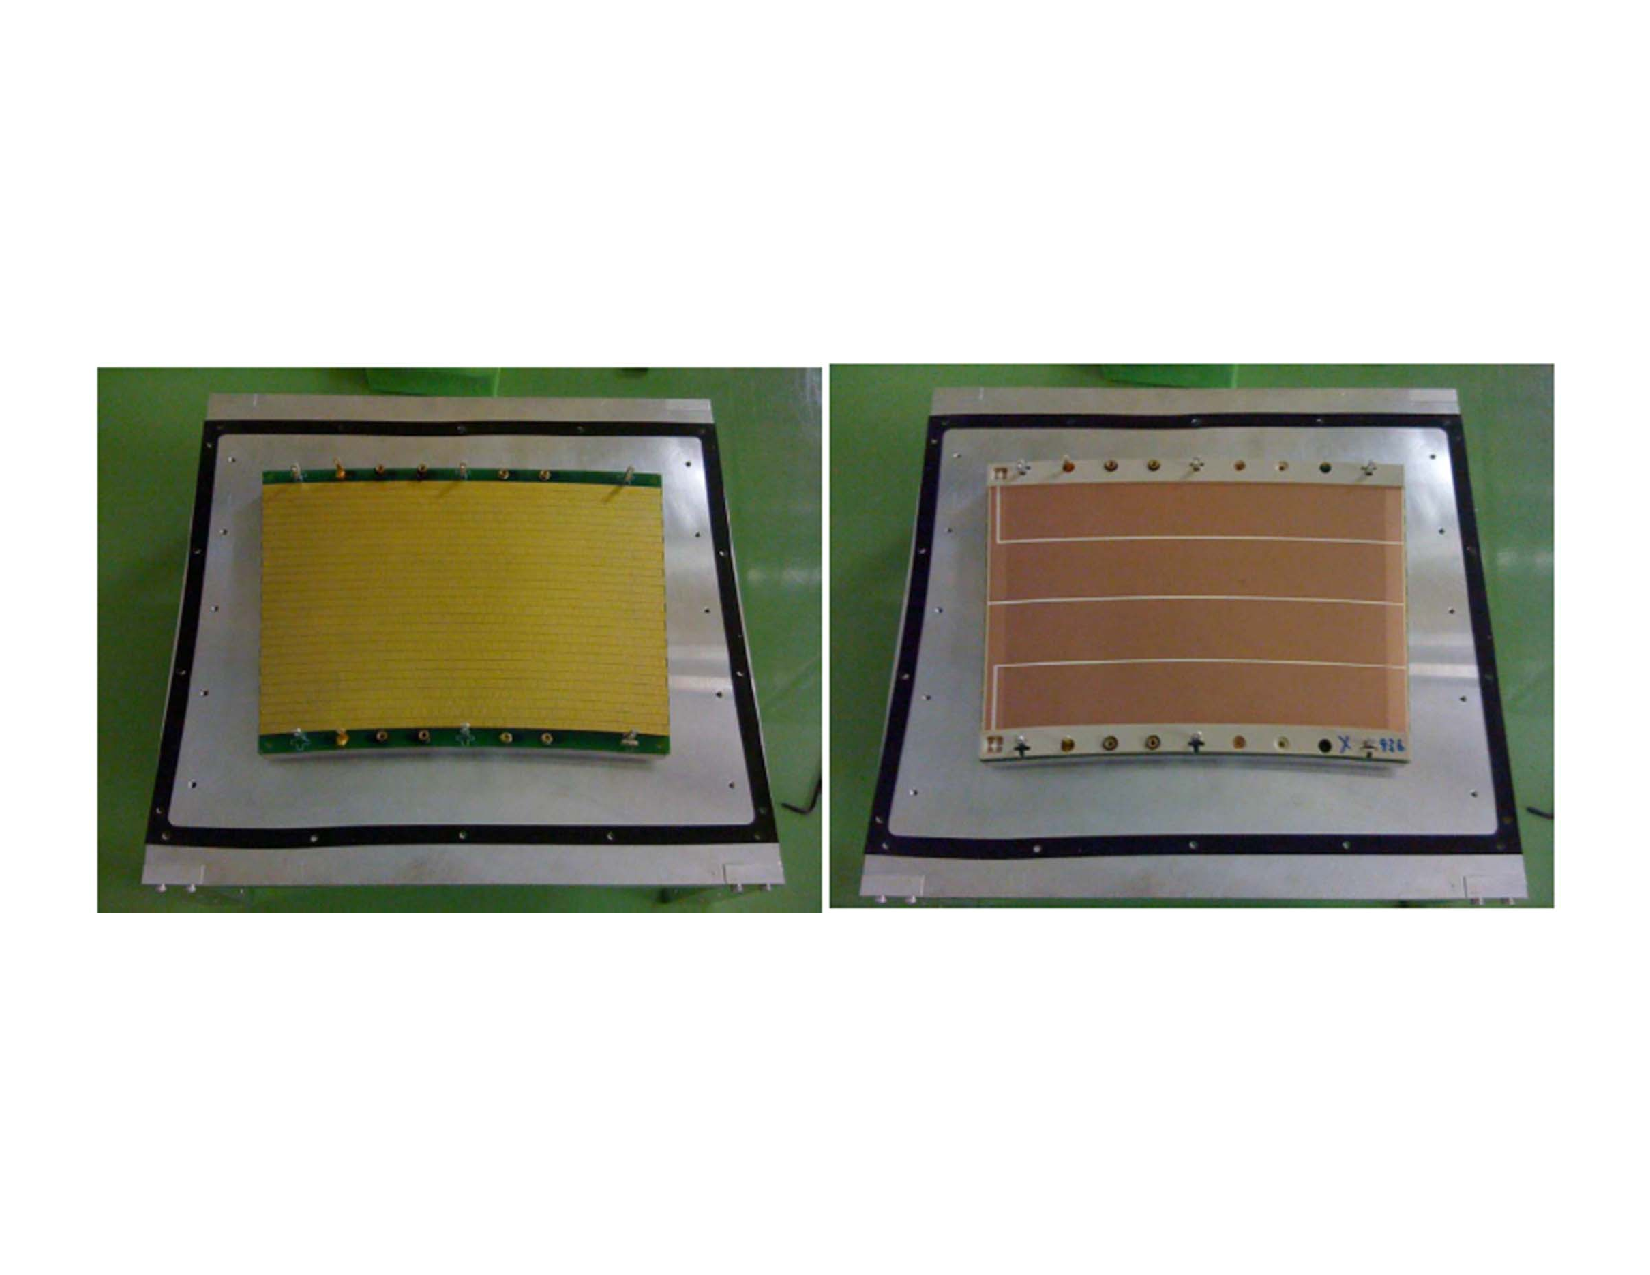
\includegraphics[width=0.9\textwidth]{plots/TPC-AG_Fig1asaingempicture.pdf}
  \caption{Asian GEM picture: left - anode pad plane; right - segmented cathode.}
  \label{fig_Fig1asiangempicture}
\end{figure}

Particles from the interaction point passing
between the modules may not be detected if they have very high momenta. Therefore, the Asian module foresees no frame along
the sides and extends the sensitive
area up to the edge of the backframe. To ensure a flat mounting of the GEMs, they are stretched on both the upper
and lower arcs (as seen in figure \ref{fig_Fig1asiangempicture}) which are made of a stiffer material:
GEMs with an insulator of \SI{100}{\micro\meter} Liquid Crystal Polymer (LCP)
covered with \SI{5}{\micro\meter} copper on both sides were produced by a company named SciEnergy.
The holes were
produced by CO$_2$-laser drilling after which they were carefully cleaned by dry etching to remove potentially
conductive residuals from the insides of the holes. The
hole pattern is identical to standard CERN GEMs. Because of the thicker material also higher gas gains per GEM
can be reached and a double GEM
structure is used and considered to be sufficient.
The two GEMs are mounted with an induction gap of \SI{2}{\milli\meter} and a transfer gap of \SI{3}{\milli\meter}.

The pad size is $1.2 \times \SI{5.4}{\milli\meter}$ and there are 28 pad rows with a total of 5152 pads.
From the beginning the use of an ion gate
(see subsection \ref{chap:TPC_sec:gating}) was envisaged and, thus, the level of the first GEM was designed
to be 1 cm below the nominal module height allowing for a later addition of the gate. To absorb the strength necessary
to stretch the GEMs and the gate, strong metal poles were implemented at the top and bottom arc.

\subsubsection{Recent Milestones}

All modules have been tested in the Large Prototype at DESY. The experience gained during all test beam periods as
well as the best transverse spatial resolution is described next. The testbeam measurements have used
the gas mixture of Ar-CF4(3\%)-isobutane(2\%). The electric drift field was set in most cases to
E=\SI{230}{\volt\per\centi\meter}, which is close to the maximum of the drift velocity, and alternatively to
E=\SI{130}{\volt\per\centi\meter}, which is the minimum of the transverse diffusion.
The Asian modules were also measured using a laser system, in order to analyse the distortions.
The laser beam was scanned across the module, and the deviations were compared with calculations and are understood.

The Asian groups built three modules and made several test beam measurements at DESY (2009, 2010, 2012).
The first campaigns were dominated by very strong field distortions because of the mounting pins and the bare frames.
After introducing the field shaper, the distortions are comparable to the ones of other techniques used for modules.
The transverse spatial resolution is shown in figure \ref{fig_Fig2asiangemresolution}, where the measured spatial
resolution of a single row in the middle of a module can be seen.

\begin{figure}[!htb]
  \centering
  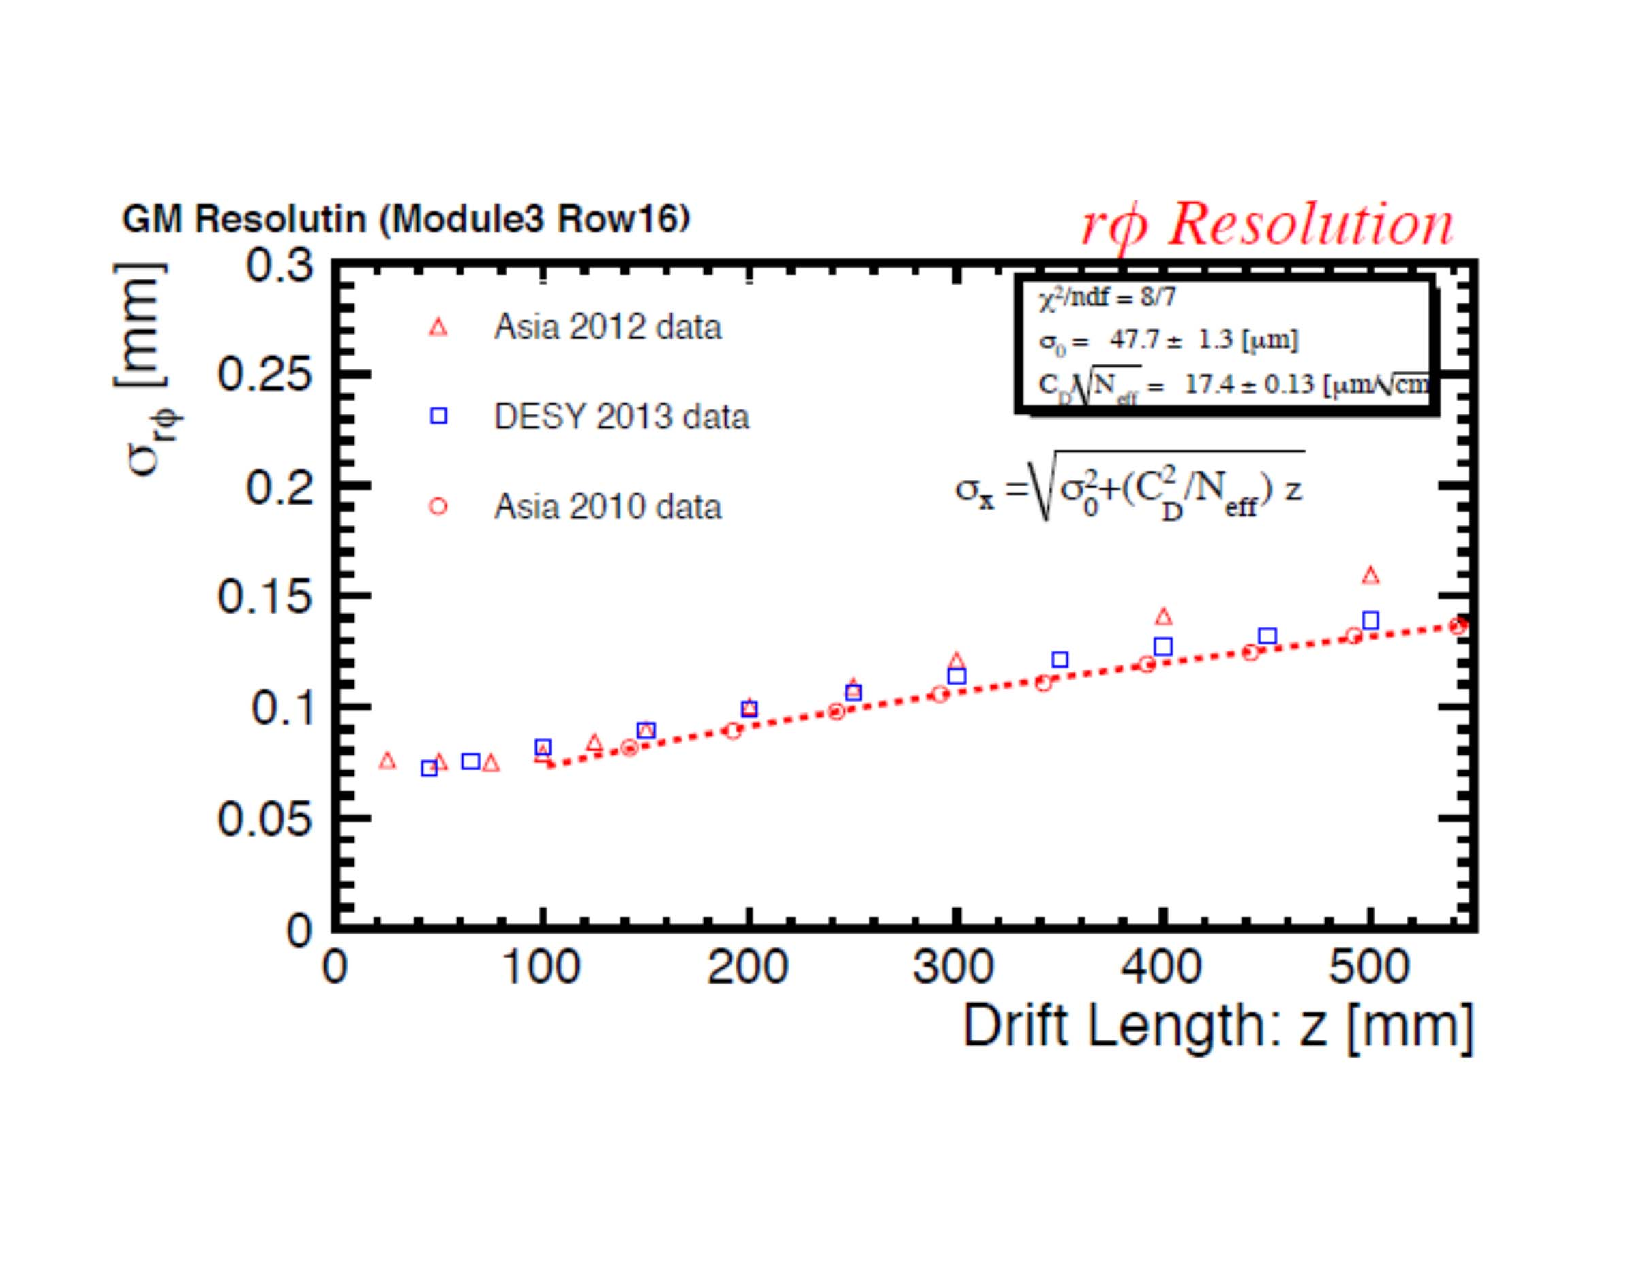
\includegraphics[width=0.9\textwidth]{plots/TPC-AG_Fig2asiangemresolution.pdf}
  \caption{Resolution measured for the Asian GEMs, and compared with a result for the DESY GEMs.}
  \label{fig_Fig2asiangemresolution}
\end{figure}

In this context an analytical formula was developed to predict the spatial resolution of a TPC. This formula includes
not only the effect of diffusion, angle,
noise and a finite pad-size, but also the influence of the electronics threshold, number of effective primary electrons,
the Polya-parameter of the gas
amplification, cross talk between pads and signal lines, charge loss because of attachment and the pad response function
are taken into account. All
these parameters can be varied and, if correctly chosen, describe well the measured data.

Finally, one other important observation was the HV microdischarges on the Asian GEMs, with associated gain drops,
and investigations of this problem are summarized here.

To minimize the energy released in a discharge, the GEMs were segmented into four arcs, each with an area of
about \SI{100}{\centi\meter\squared} (figure \ref{fig_Fig1asiangempicture}, right).
Studies of the microdischarges for the various types of GEMs were measured under a controlled environment.
The \SI{100}{\micro\meter} Asian GEMs discharged frequently, while the DESY \SI{50}{\micro\meter} GEMs (made by CERN) had little or no
discharges. For the \SI{50}{\micro\meter} GEMs, there is no significant difference of
the discharge rate between different types of GEMs. It is noteworthy that, at low gain, the \SI{100}{\micro\meter} GEMs
had a discharge rate which is almost the same as for the \SI{50}{\micro\meter} GEMs. The water content in the gas does not seem to
influence the
discharge rate, and long-term measurements are in progress.


\subsubsection{Future Plans}

In the future, it is planned to:\\
$\bullet$ understand better the reasons for the micro discharges and eliminate them, and \\
$\bullet$ construct a full scale Asian module with gate.

%\label{chap:TPC_sec:DESY_gems}
Contact person: Ties Behnke (email: ties.behnke\@ desy.de)\\

The goal of module type-B is a maximal coverage of the endplate with minimal dead area and a low material budget. It relies on thin ceramic frames to support the GEM foils on top of the readout plane \cite{HallermannPhD,DESYGEM}, see figure \ref{fig:moduleAssembled}. The high stiffness of the ceramic frame allows the construction of very thin frames, which in turn minimize the dead areas of the module. With the current design only $\sim5\%$ of the active area is taken by the support structure and gaps between modules, the rest is sensitive area. The design of the system allows the simple stacking of GEM foils to build up compact, light weight self supporting multi-GEM modules. The development of this module type is led by DESY.

\begin{figure}[htb!]
\begin{subfigure}[b]{0.48\textwidth}
\includegraphics[width=\textwidth]{plots/TPC-DG_GemModule_Explosion.pdf}
\caption{}
\label{sfig:moduleExp}
\end{subfigure}
\hfill
\begin{subfigure}[b]{0.48\textwidth}
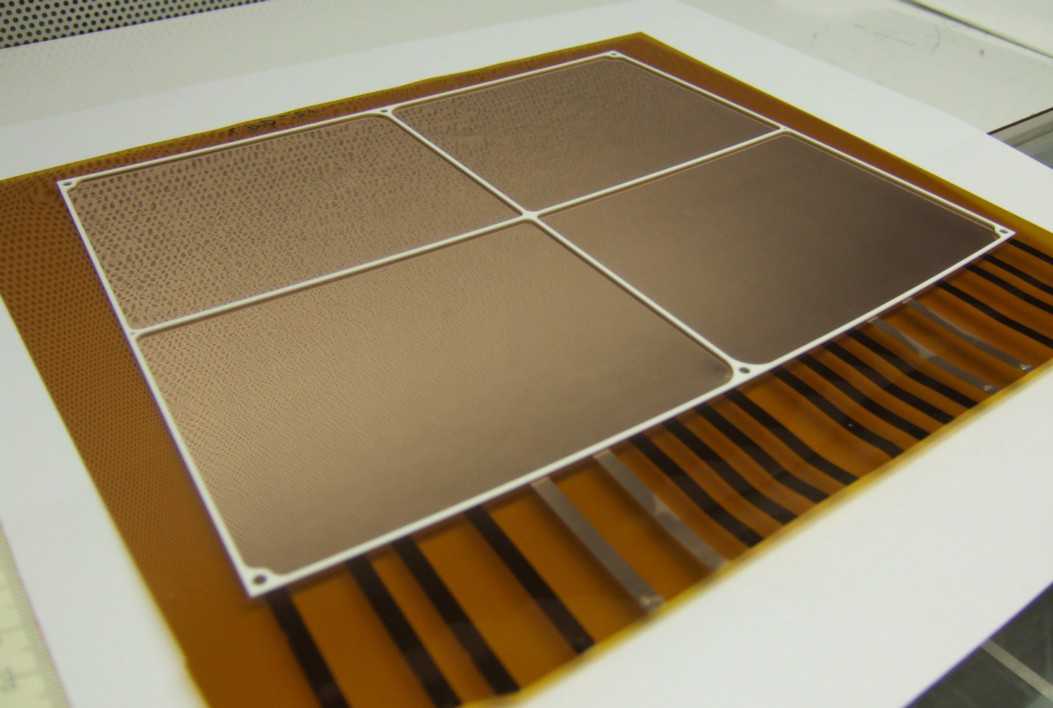
\includegraphics[width=\textwidth]{plots/TPC-DG_GemGrid.png}
\caption{}
\label{sfig:moduleGEM}
\end{subfigure}
\caption [Readout Module GEM]{\small \protect\subref{sfig:moduleExp})~Exploded view of one module showing the sequence of GEM foils and ceramic frames. \protect\subref{sfig:moduleGEM})~GEM foil with ceramic frame support used in the construction of the modules.}
\label{fig:moduleAssembled}
\end{figure}

\subsubsection{Recent Milestones}
Over the last years several test-beam campaigns took place and exposed three GEM based modules to test beam. Extensive data sets were collected with and without magnetic field, at different working points, and at different angles between the TPC and the beam.

For the first time the data taken were used in a global attempt to determine and correct field distortions. The Millepede-II \cite{millepedeNIM,millepedeWiki} program was used to perform this global fit. First results indicate that distortions as large as several millimeters can be well corrected, see figure \ref{sfig:1Tdistort}. The resolution obtained both in $r\text{-}\varphi$ and $z$ behave as expected, and, if extrapolated to the running conditions at the ILC, meet the requirements, see figure \ref{sfig:resextrapol}.

\begin{figure}[htb!]
\begin{subfigure}[b]{0.48\textwidth}
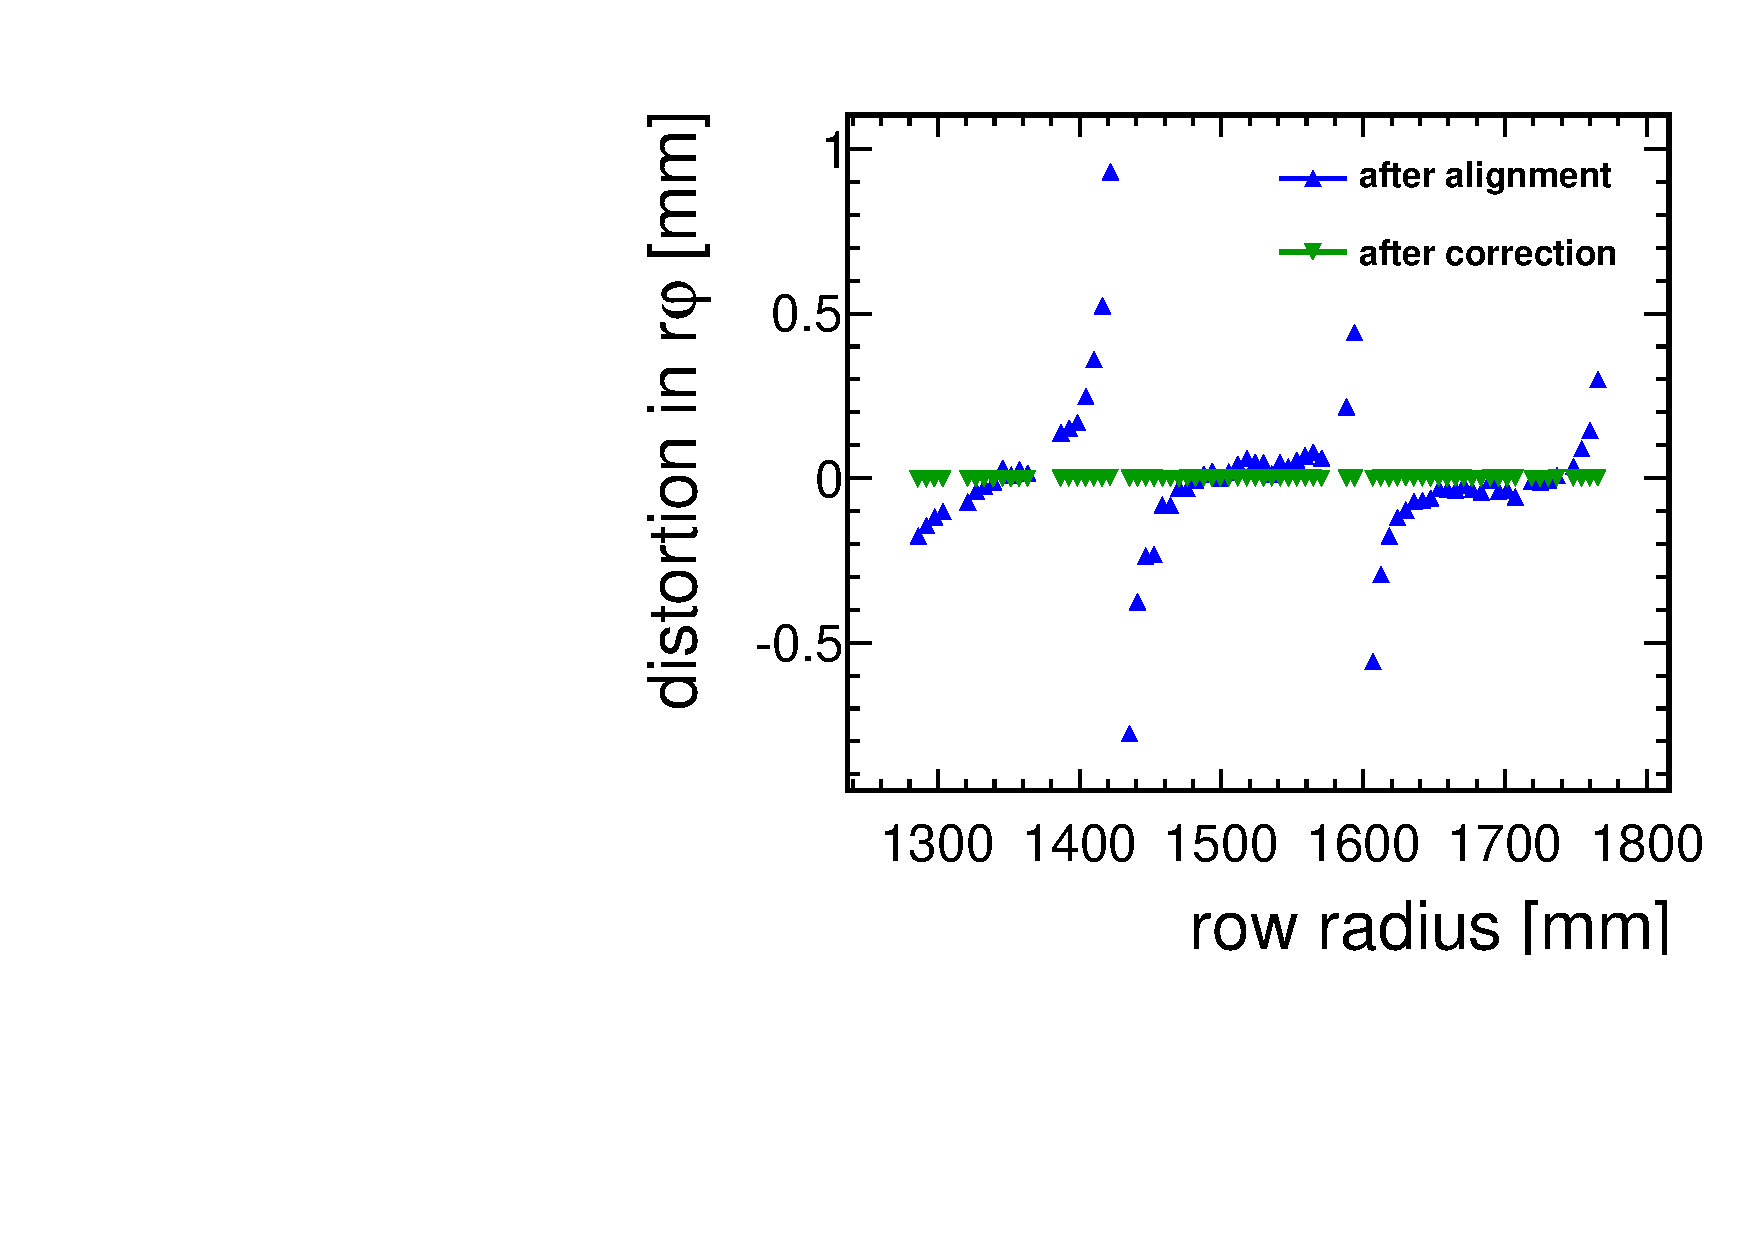
\includegraphics[width=\textwidth]{plots/TPC-DG_distortionAlignmentPaper1Tdistcor.pdf}
\caption{}
\label{sfig:1Tdistort}
\end{subfigure}
\begin{subfigure}[b]{0.48\textwidth}
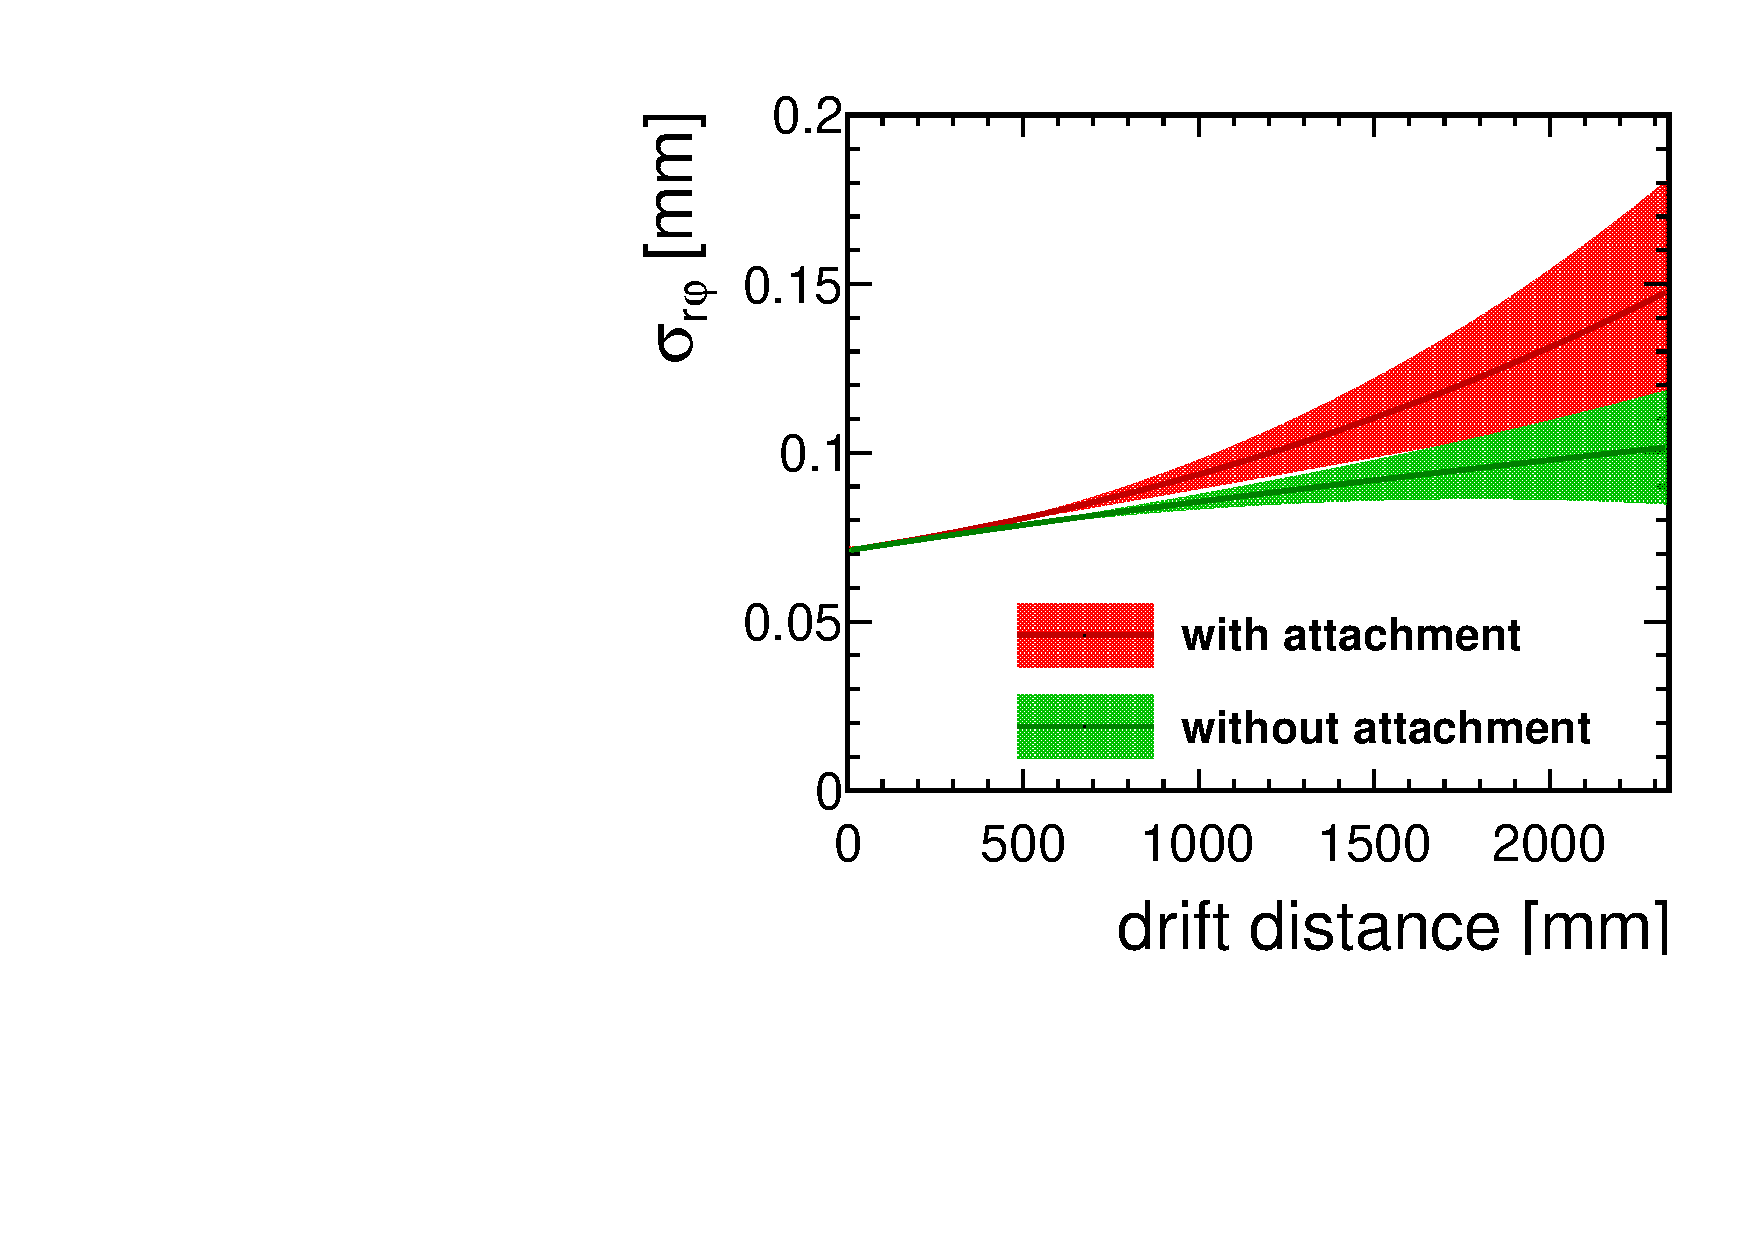
\includegraphics[width=\textwidth]{plots/TPC-DG_xyResolutionExtrapolated.pdf}
\caption{}
\label{sfig:resextrapol}
\end{subfigure}
\caption{\small \protect\subref{sfig:1Tdistort})~Alignment and distortion correction: mean hit position in $r\varphi$ with respect to the track position at \SI{1}{\tesla} versus pad row radius. In blue after alignment correction, in green after distortion correction. \protect\subref{sfig:resextrapol})~Point resolution: extrapolation to a magnetic field of \unit[3.5]{T} based on parameters measured with the Large TPC Prototype at \unit[1.0]{T}. Plotted over the full ILD TPC drift length of \unit[2.35]{m} including \unit[1]{$\sigma$} error bands. In red with the measured attachment rate, in green without any attachment.}
\label{fig:align1Tdistort}
\end{figure}

The field homogeneity was in addition studied in dedicated laser runs \cite{ZenkerPhD}. A UV laser illuminates the cathode plane in the TPC, on which dots are placed made from a material with a small work function. The laser light extracts electrons at the position of the dots. These electrons are then drifted towards the anode, and are measured. From the dislocations of the dots relative to the known position on the cathode, the integrated effect of field distortions in the TPC volume can be measured.

Extensive simulations of the behavior of the GEM foils in case of electrical breakdown were performed. They showed that a strong coupling exists between the different regions of the GEM foil. In some cases these couplings can trigger secondary trips in the module, which in rare cases can damage the GEM. A protection circuit is currently under development and will be tested in the near future.

%\subsubsection{Engineering Challenges}
\subsubsection{Future Plans}

By now two generations of these modules have been developed and successfully tested. The main issues which are going to be addressed in the next 1-2 years are
\begin{itemize}
\item re-optimisation of the support structure for maximum mechanical strength and minimal interference with the readout
\item development of a protection scheme which will ensure safe operation of the module even in case of high-voltage trips.
\item optimization of the field-shaping integrated into the module, to minimize field distortions close to the module and at module boundaries.
\item integration of a GEM based gate on top of the current amplification structure, based on the recent developments at KEK.
\end{itemize}
It is planned that within the next six months a third generation module design will be developed and several modules built which will address these challenges.

\subsubsection{Engineering Challenges}
%The GEM based modules face rather similar engineering challenges. Among the most important one is the optimisation of the overall mechanical structure, to provide adequate mechanical strength, without introducing excess dead material.
A detailed study is ongoing to understand and quantify the mechanical behavior of the ceramic frame GEM system. Bending tests have been performed, and compared to simulations. The interference between the mechanical properties and the electrical properties are studied. Measurements of the flatness of the module are being done, and will provide input for the next design iteration.
The fabrication of the ceramic frames which is currently done by laser cutting from solid sheets of ceramic will be studied. Possible alternatives are 3D printing of the frames. Improvements in the laser cutting technology might allow thinner frames, without loosing stiffness.

Another open question is the distribution of the high voltage from the endplate to the different GEM layers. The current solution is rather labour intensive, and relies heavily on the skills of the person doing this connection. Faults are difficult to find, and even more difficult to repair. Here new solutions are being sought, which are more easily to produce, more reliable, and will give better high voltage security. Connected to this are the protection schemes against accidental high voltage discharges, which are still not perfect.

As discussed in section \ref{chap:TPC_sec:gating}, a gating GEM will be implemented as part of the amplification scheme. This gating GEM needs to be mechanically integrated into the module.

Currently a gap of about \SI{2}{\milli\meter} exists between neighbouring modules. This gap introduces significant field distortions \cite{ZenkerPhD}. They are partially compensated by a field shaping strip on the outside of each module. However a better and more robust solution would be to further minimise the gap between modules. Doing so will need improvements of the high voltage distribution, as discussed above, but also of the overall mechanical integration of the modules into the endplate.

%\subsection{Applications Outside of Linear Colliders}

\subsection{GEM based Readout}\label{chap:TPC_sec:standard_gems}

Gas Electron Multipliers (GEMs) \cite{Sauli_GEM} have been invented in the mid 90's. They consist of a thin polyamid foil, covered with Copper on both sides. Holes are produced into the foil on a regular pattern. Typical dimensions are a hole pitch of \unit[140]{\mu m} and a hole diameter of \unit[70]{\mu m}. If an electric field is applied between the two sides of the foil, high fields form inside the holes, and provide avalanche gas amplification. Since the high fields are constrained inside the holes, many of the high-voltage problems connected to traditional wire based chambers are not relevant. GEM foils can be stacked to provide tailored gas amplification. During the years a number of different types of GEM foils have been developed. They differ for example in the cross section of the holes, in the material of the foil, and in the pitch and hole sizes. For application in the ILC TPC currently two main options are being pursued. The first one is based on a GEM where a laser is used to ``drill'' each hole.
The resulting holes are
strictly cylindrical. The second option is based on a chemical etching process. The resulting holes have a double conical shape.

In addition to the different types of GEM foils two different schemes to build readout modules for the TPC are investigated. Scheme one (called module type A in the following) relies on a sturdy aluminium frame where the GEM foils are stretched between the bottom and the top of the readout module. This scheme allows to build a module which has essentially no dead area on the side of the module, but where some dead space is needed on the top and the bottom. The second option (called module type B in the following) relies on an assembly of a stiff but thin ceramic frame which when glued to the GEM provides a self-supporting stiff assembly. The width of the frame is around one millimetre, so that in this approach a small dead area is present all around the module. Both approaches allow the stacking of GEM foils, and both are compatible with the installation of a gating GEM on top.

\subsubsection{Module Type A, ``Asian Module''}
%\section{Asian GEM}
\label{chap:TPC_sec:asian_gems}
Contact person: Akira Sugiyama(email: sugiyama@cc.saga-u.ac.jp)\\

%\subsection{Engineering Challenges}

The Asian modules use GEM stacks as a gas amplification stage and are optimised to reduce the insensitive area
on the sides of the modules which point towards the detector center.
A module can be seen in figure \ref{fig_Fig1asiangempicture}.

\begin{figure}[!htb]
  \centering
  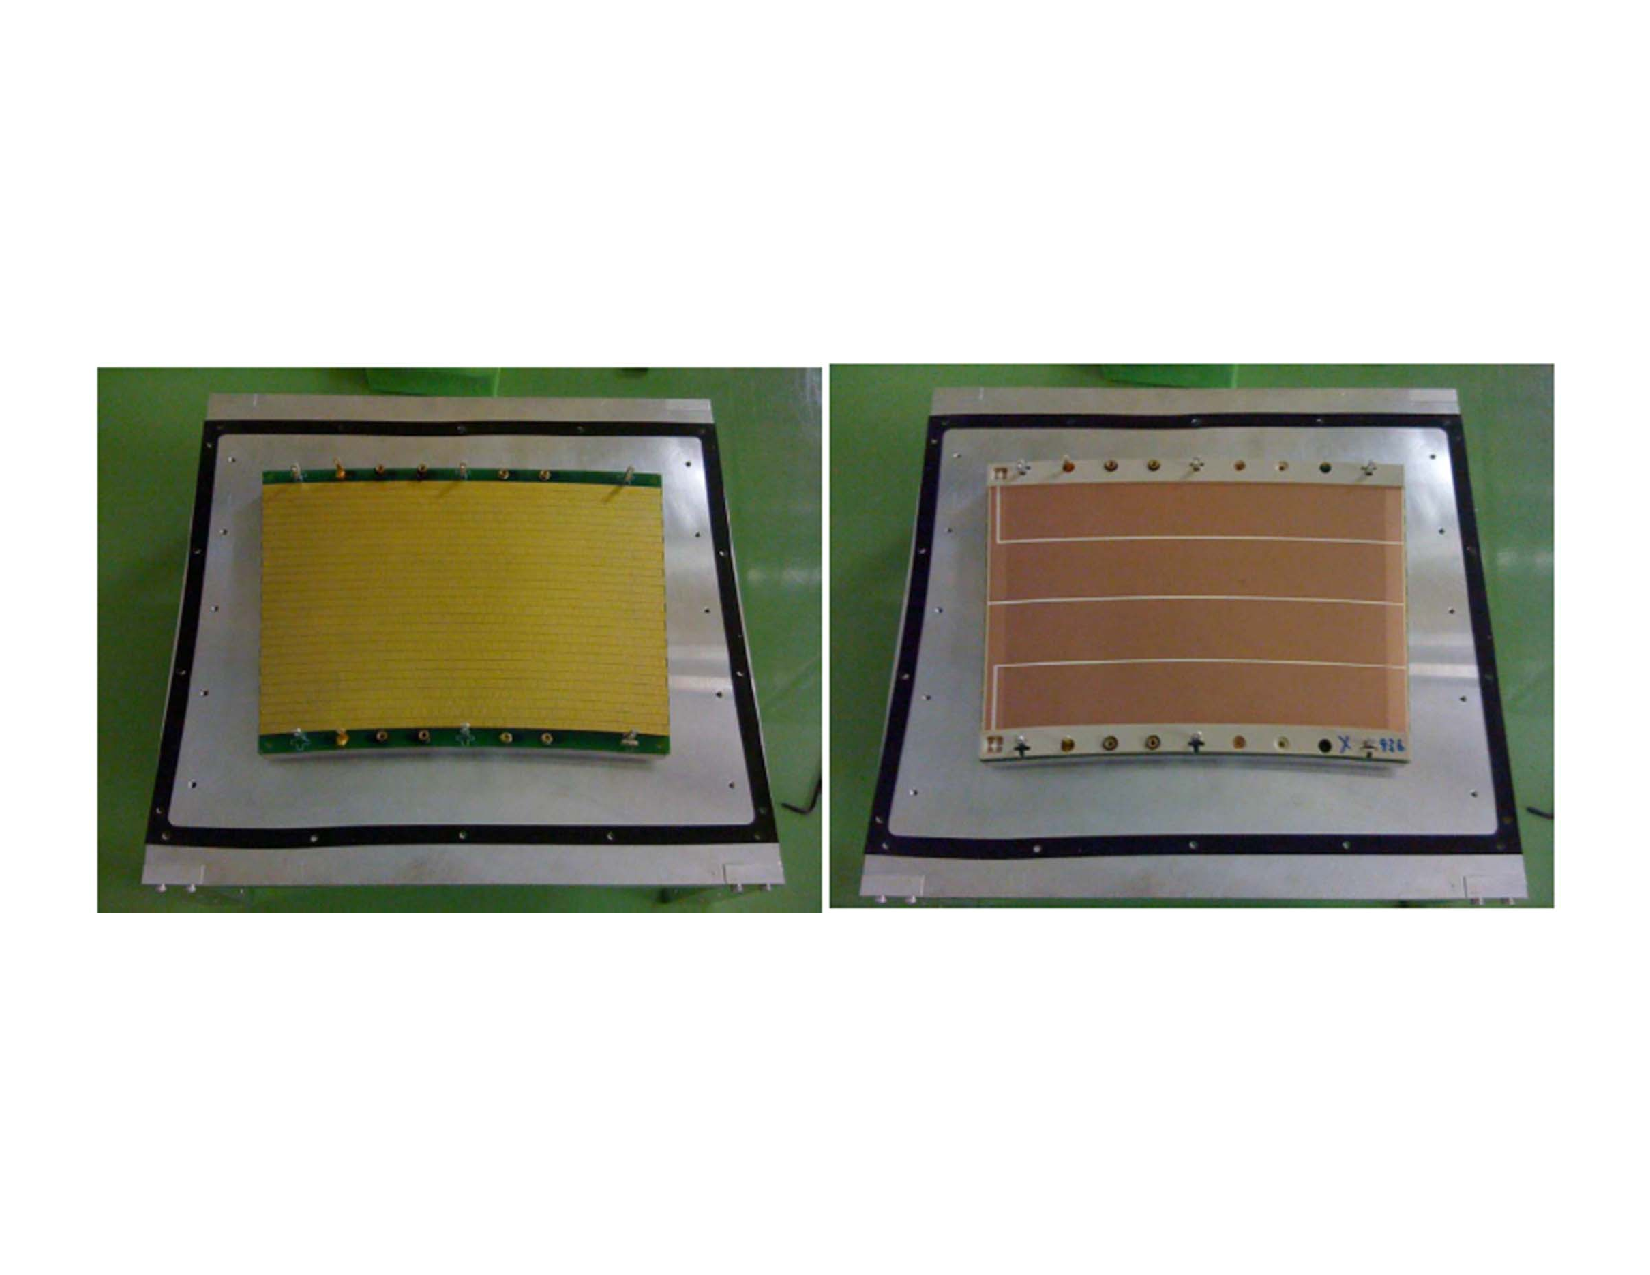
\includegraphics[width=0.9\textwidth]{plots/TPC-AG_Fig1asaingempicture.pdf}
  \caption{Asian GEM picture: left - anode pad plane; right - segmented cathode.}
  \label{fig_Fig1asiangempicture}
\end{figure}

Particles from the interaction point passing
between the modules may not be detected if they have very high momenta. Therefore, the Asian module foresees no frame along
the sides and extends the sensitive
area up to the edge of the backframe. To ensure a flat mounting of the GEMs, they are stretched on both the upper
and lower arcs (as seen in figure \ref{fig_Fig1asiangempicture}) which are made of a stiffer material:
GEMs with an insulator of \SI{100}{\micro\meter} Liquid Crystal Polymer (LCP)
covered with \SI{5}{\micro\meter} copper on both sides were produced by a company named SciEnergy.
The holes were
produced by CO$_2$-laser drilling after which they were carefully cleaned by dry etching to remove potentially
conductive residuals from the insides of the holes. The
hole pattern is identical to standard CERN GEMs. Because of the thicker material also higher gas gains per GEM
can be reached and a double GEM
structure is used and considered to be sufficient.
The two GEMs are mounted with an induction gap of \SI{2}{\milli\meter} and a transfer gap of \SI{3}{\milli\meter}.

The pad size is $1.2 \times \SI{5.4}{\milli\meter}$ and there are 28 pad rows with a total of 5152 pads.
From the beginning the use of an ion gate
(see subsection \ref{chap:TPC_sec:gating}) was envisaged and, thus, the level of the first GEM was designed
to be 1 cm below the nominal module height allowing for a later addition of the gate. To absorb the strength necessary
to stretch the GEMs and the gate, strong metal poles were implemented at the top and bottom arc.

\subsubsection{Recent Milestones}

All modules have been tested in the Large Prototype at DESY. The experience gained during all test beam periods as
well as the best transverse spatial resolution is described next. The testbeam measurements have used
the gas mixture of Ar-CF4(3\%)-isobutane(2\%). The electric drift field was set in most cases to
E=\SI{230}{\volt\per\centi\meter}, which is close to the maximum of the drift velocity, and alternatively to
E=\SI{130}{\volt\per\centi\meter}, which is the minimum of the transverse diffusion.
The Asian modules were also measured using a laser system, in order to analyse the distortions.
The laser beam was scanned across the module, and the deviations were compared with calculations and are understood.

The Asian groups built three modules and made several test beam measurements at DESY (2009, 2010, 2012).
The first campaigns were dominated by very strong field distortions because of the mounting pins and the bare frames.
After introducing the field shaper, the distortions are comparable to the ones of other techniques used for modules.
The transverse spatial resolution is shown in figure \ref{fig_Fig2asiangemresolution}, where the measured spatial
resolution of a single row in the middle of a module can be seen.

\begin{figure}[!htb]
  \centering
  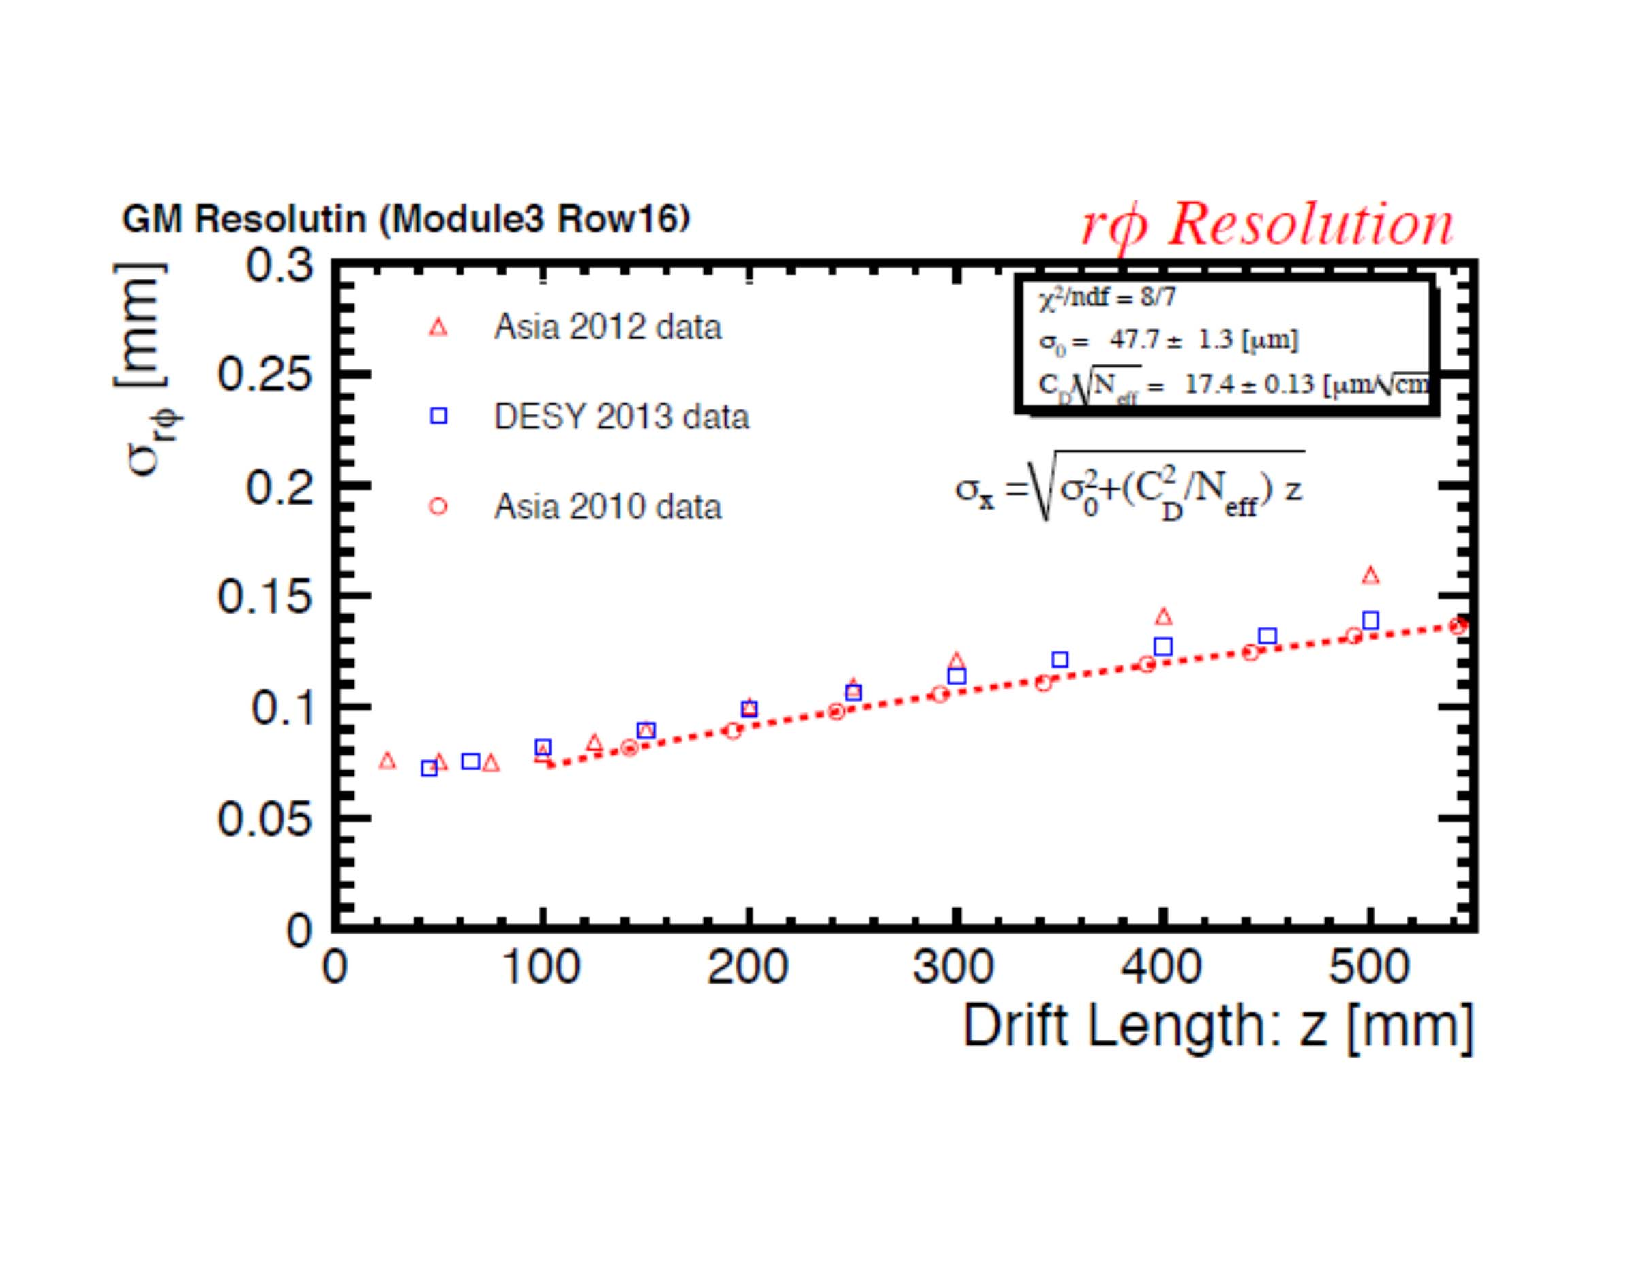
\includegraphics[width=0.9\textwidth]{plots/TPC-AG_Fig2asiangemresolution.pdf}
  \caption{Resolution measured for the Asian GEMs, and compared with a result for the DESY GEMs.}
  \label{fig_Fig2asiangemresolution}
\end{figure}

In this context an analytical formula was developed to predict the spatial resolution of a TPC. This formula includes
not only the effect of diffusion, angle,
noise and a finite pad-size, but also the influence of the electronics threshold, number of effective primary electrons,
the Polya-parameter of the gas
amplification, cross talk between pads and signal lines, charge loss because of attachment and the pad response function
are taken into account. All
these parameters can be varied and, if correctly chosen, describe well the measured data.

Finally, one other important observation was the HV microdischarges on the Asian GEMs, with associated gain drops,
and investigations of this problem are summarized here.

To minimize the energy released in a discharge, the GEMs were segmented into four arcs, each with an area of
about \SI{100}{\centi\meter\squared} (figure \ref{fig_Fig1asiangempicture}, right).
Studies of the microdischarges for the various types of GEMs were measured under a controlled environment.
The \SI{100}{\micro\meter} Asian GEMs discharged frequently, while the DESY \SI{50}{\micro\meter} GEMs (made by CERN) had little or no
discharges. For the \SI{50}{\micro\meter} GEMs, there is no significant difference of
the discharge rate between different types of GEMs. It is noteworthy that, at low gain, the \SI{100}{\micro\meter} GEMs
had a discharge rate which is almost the same as for the \SI{50}{\micro\meter} GEMs. The water content in the gas does not seem to
influence the
discharge rate, and long-term measurements are in progress.


\subsubsection{Future Plans}

In the future, it is planned to:\\
$\bullet$ understand better the reasons for the micro discharges and eliminate them, and \\
$\bullet$ construct a full scale Asian module with gate.

\subsubsection{Module type B, ``DESY Module''}
\label{chap:TPC_sec:DESY_gems}
Contact person: Ties Behnke (email: ties.behnke\@ desy.de)\\

The goal of module type-B is a maximal coverage of the endplate with minimal dead area and a low material budget. It relies on thin ceramic frames to support the GEM foils on top of the readout plane \cite{HallermannPhD,DESYGEM}, see figure \ref{fig:moduleAssembled}. The high stiffness of the ceramic frame allows the construction of very thin frames, which in turn minimize the dead areas of the module. With the current design only $\sim5\%$ of the active area is taken by the support structure and gaps between modules, the rest is sensitive area. The design of the system allows the simple stacking of GEM foils to build up compact, light weight self supporting multi-GEM modules. The development of this module type is led by DESY.

\begin{figure}[htb!]
\begin{subfigure}[b]{0.48\textwidth}
\includegraphics[width=\textwidth]{plots/TPC-DG_GemModule_Explosion.pdf}
\caption{}
\label{sfig:moduleExp}
\end{subfigure}
\hfill
\begin{subfigure}[b]{0.48\textwidth}
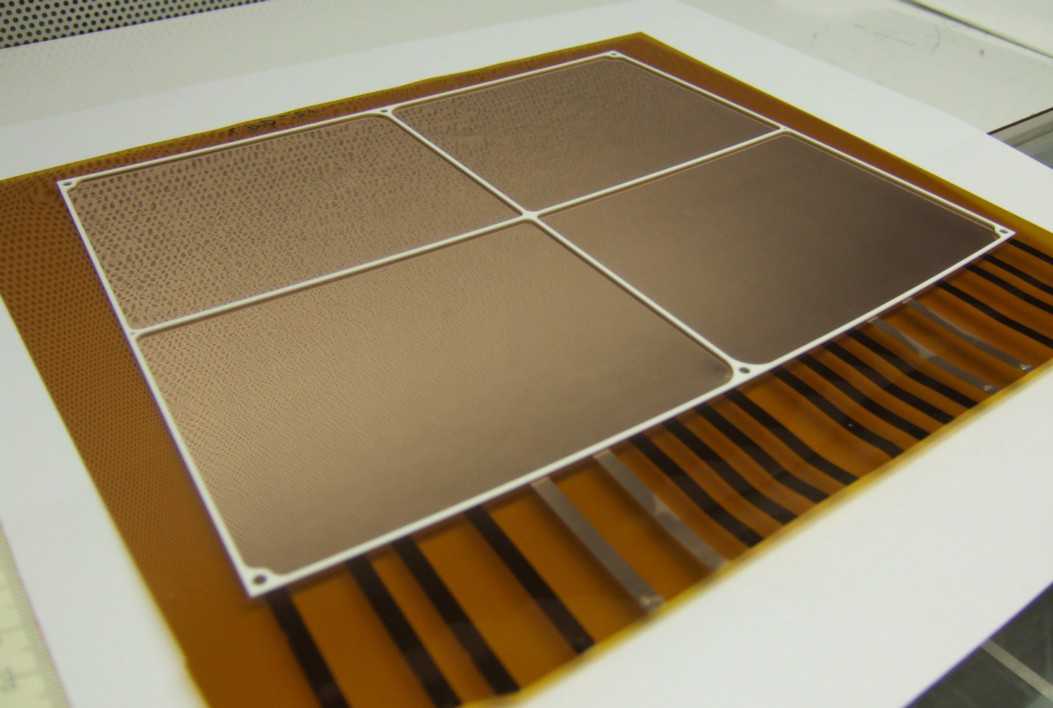
\includegraphics[width=\textwidth]{plots/TPC-DG_GemGrid.png}
\caption{}
\label{sfig:moduleGEM}
\end{subfigure}
\caption [Readout Module GEM]{\small \protect\subref{sfig:moduleExp})~Exploded view of one module showing the sequence of GEM foils and ceramic frames. \protect\subref{sfig:moduleGEM})~GEM foil with ceramic frame support used in the construction of the modules.}
\label{fig:moduleAssembled}
\end{figure}

\subsubsection{Recent Milestones}
Over the last years several test-beam campaigns took place and exposed three GEM based modules to test beam. Extensive data sets were collected with and without magnetic field, at different working points, and at different angles between the TPC and the beam.

For the first time the data taken were used in a global attempt to determine and correct field distortions. The Millepede-II \cite{millepedeNIM,millepedeWiki} program was used to perform this global fit. First results indicate that distortions as large as several millimeters can be well corrected, see figure \ref{sfig:1Tdistort}. The resolution obtained both in $r\text{-}\varphi$ and $z$ behave as expected, and, if extrapolated to the running conditions at the ILC, meet the requirements, see figure \ref{sfig:resextrapol}.

\begin{figure}[htb!]
\begin{subfigure}[b]{0.48\textwidth}
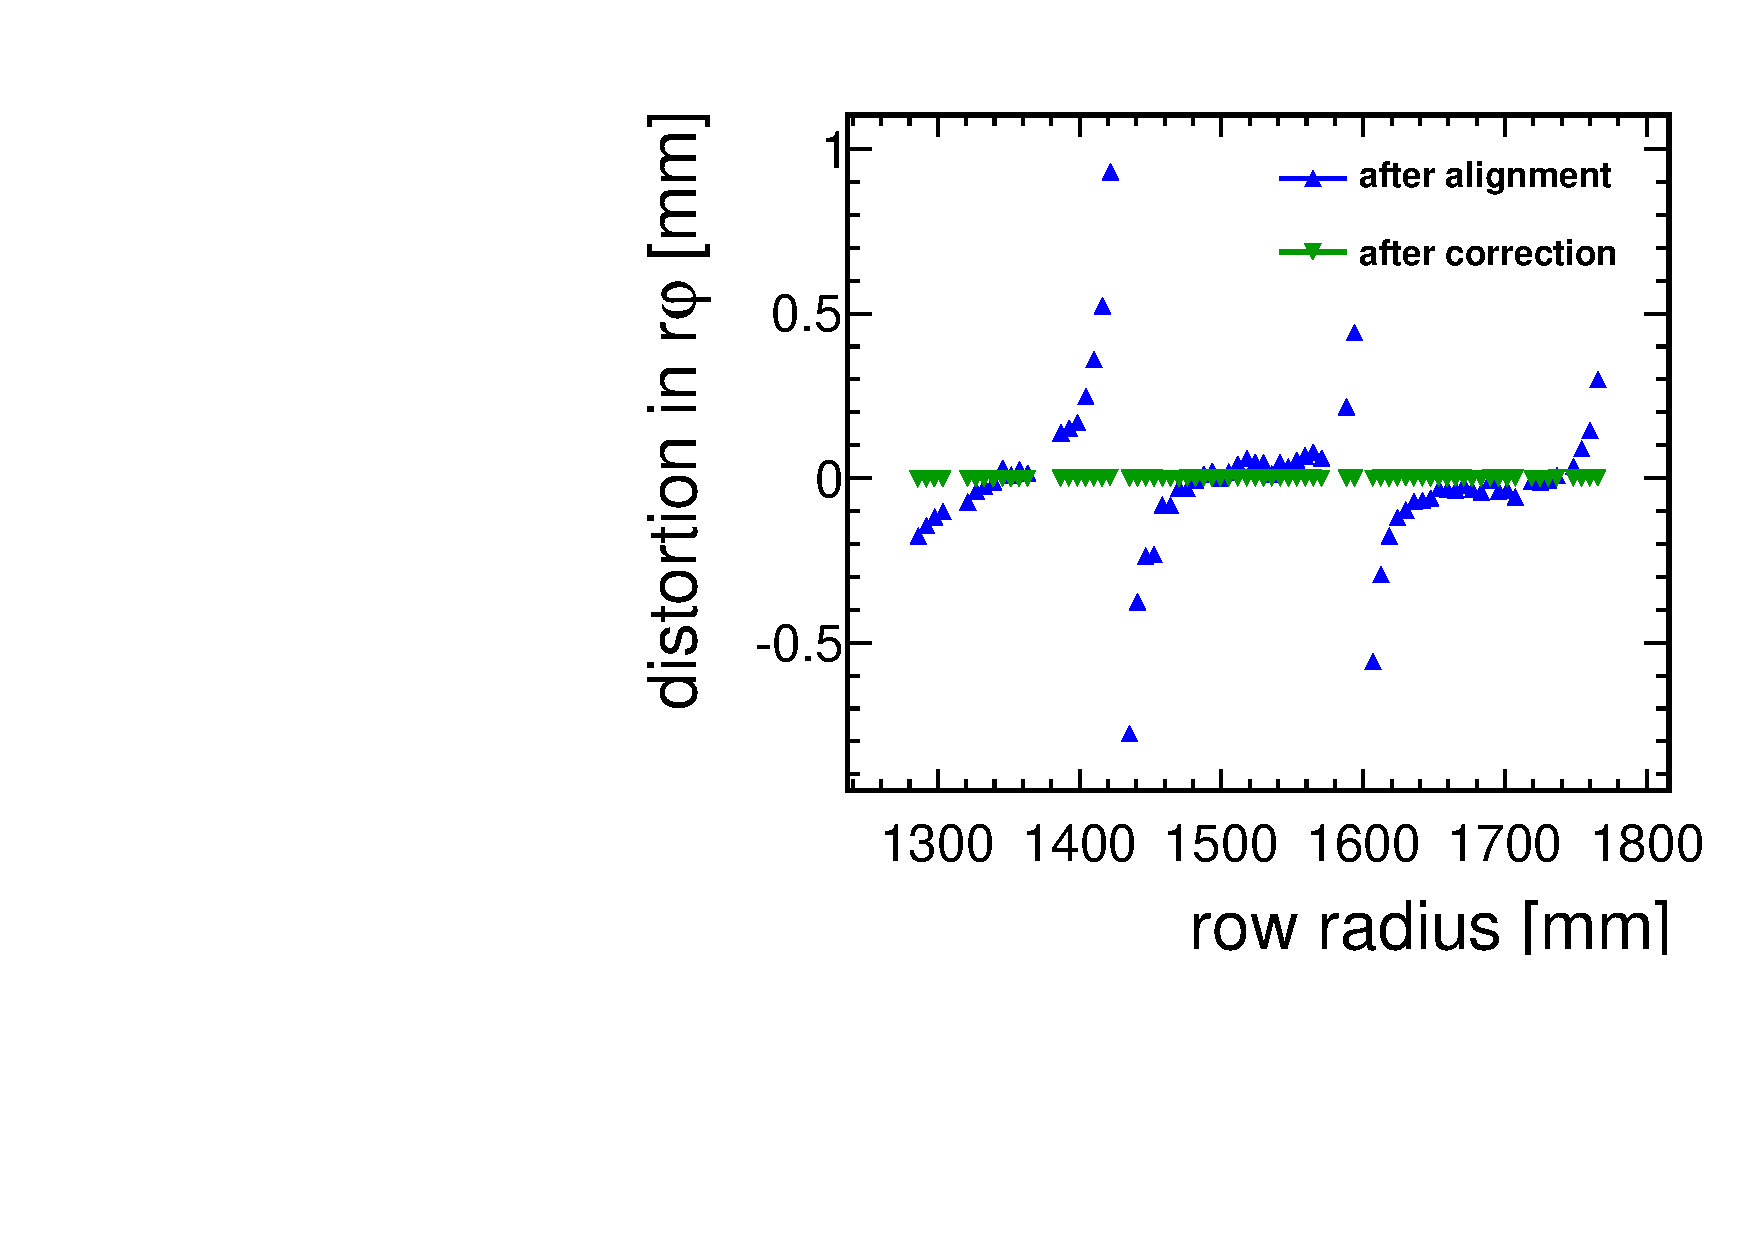
\includegraphics[width=\textwidth]{plots/TPC-DG_distortionAlignmentPaper1Tdistcor.pdf}
\caption{}
\label{sfig:1Tdistort}
\end{subfigure}
\begin{subfigure}[b]{0.48\textwidth}
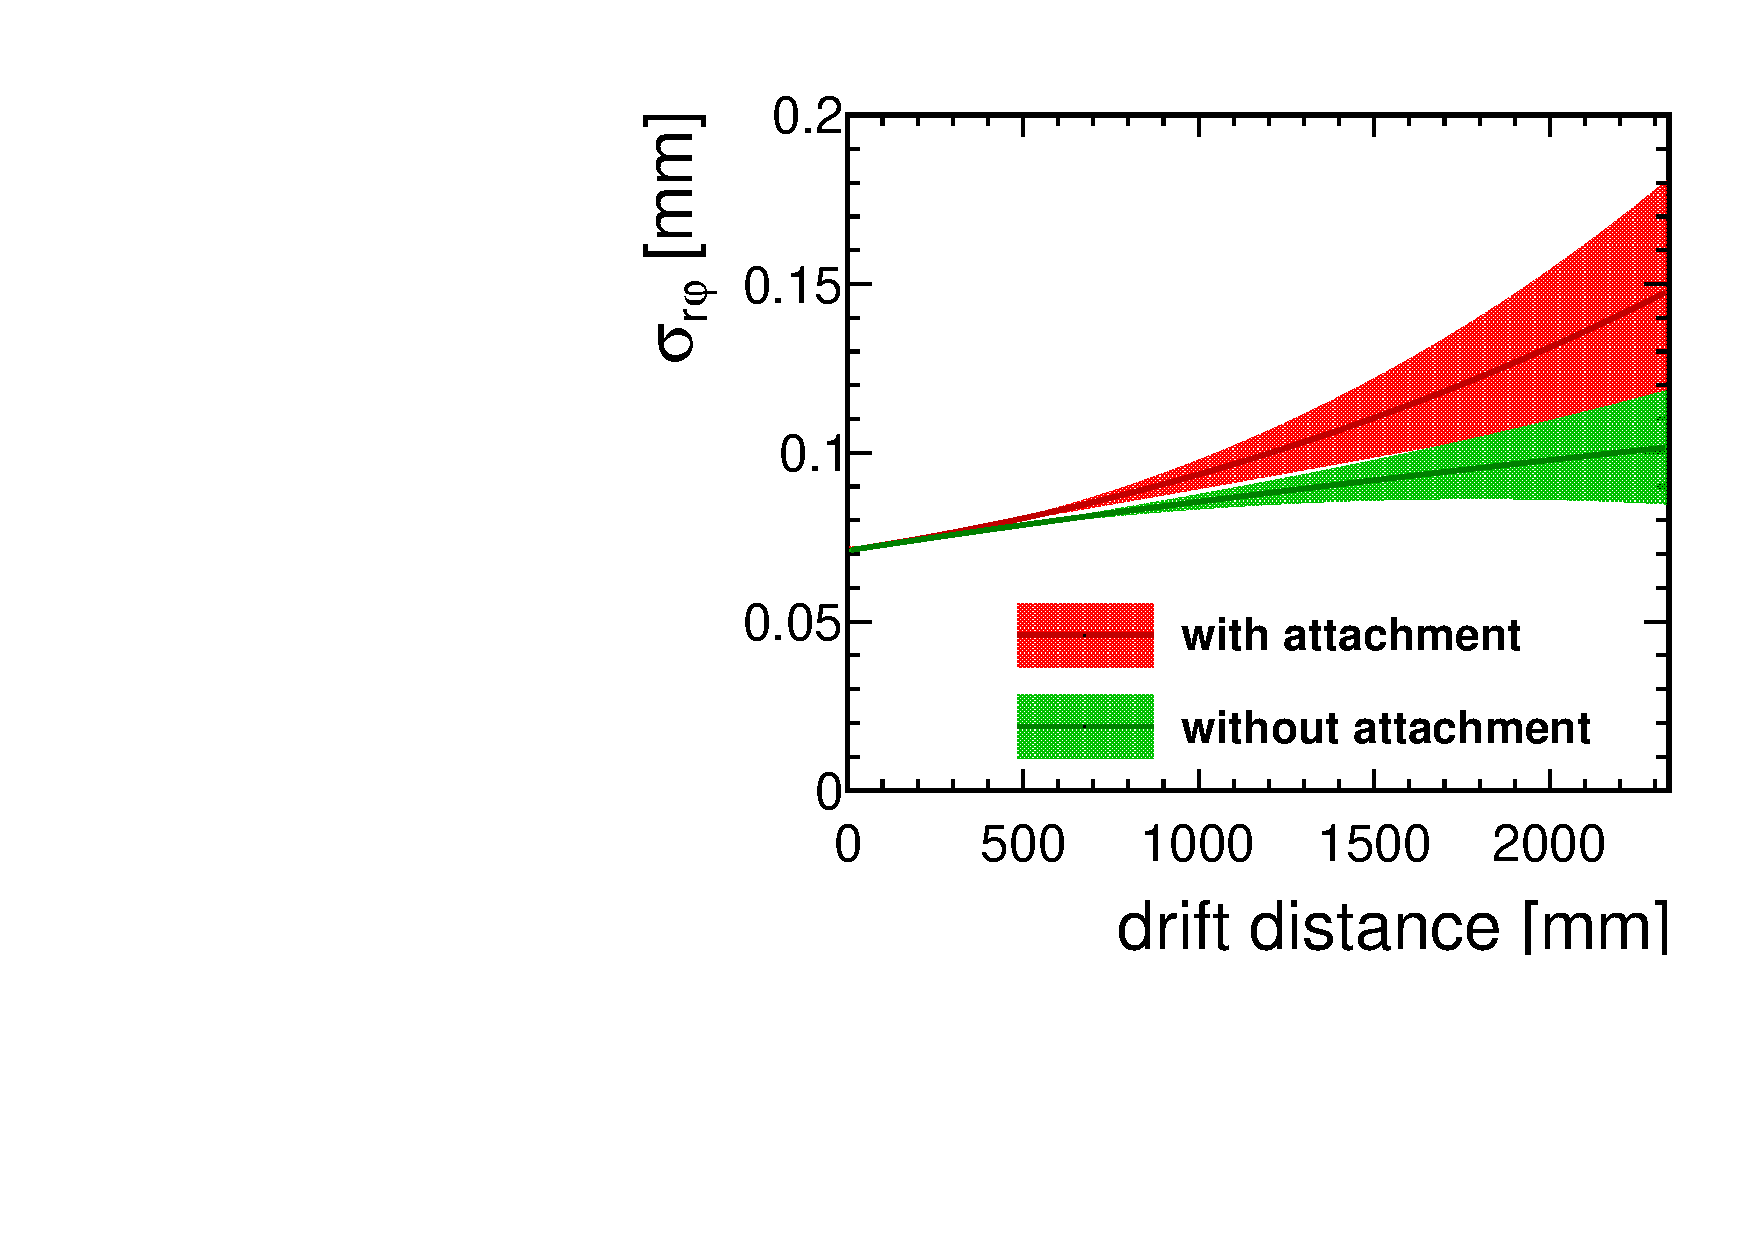
\includegraphics[width=\textwidth]{plots/TPC-DG_xyResolutionExtrapolated.pdf}
\caption{}
\label{sfig:resextrapol}
\end{subfigure}
\caption{\small \protect\subref{sfig:1Tdistort})~Alignment and distortion correction: mean hit position in $r\varphi$ with respect to the track position at \SI{1}{\tesla} versus pad row radius. In blue after alignment correction, in green after distortion correction. \protect\subref{sfig:resextrapol})~Point resolution: extrapolation to a magnetic field of \unit[3.5]{T} based on parameters measured with the Large TPC Prototype at \unit[1.0]{T}. Plotted over the full ILD TPC drift length of \unit[2.35]{m} including \unit[1]{$\sigma$} error bands. In red with the measured attachment rate, in green without any attachment.}
\label{fig:align1Tdistort}
\end{figure}

The field homogeneity was in addition studied in dedicated laser runs \cite{ZenkerPhD}. A UV laser illuminates the cathode plane in the TPC, on which dots are placed made from a material with a small work function. The laser light extracts electrons at the position of the dots. These electrons are then drifted towards the anode, and are measured. From the dislocations of the dots relative to the known position on the cathode, the integrated effect of field distortions in the TPC volume can be measured.

Extensive simulations of the behavior of the GEM foils in case of electrical breakdown were performed. They showed that a strong coupling exists between the different regions of the GEM foil. In some cases these couplings can trigger secondary trips in the module, which in rare cases can damage the GEM. A protection circuit is currently under development and will be tested in the near future.

%\subsubsection{Engineering Challenges}
\subsubsection{Future Plans}

By now two generations of these modules have been developed and successfully tested. The main issues which are going to be addressed in the next 1-2 years are
\begin{itemize}
\item re-optimisation of the support structure for maximum mechanical strength and minimal interference with the readout
\item development of a protection scheme which will ensure safe operation of the module even in case of high-voltage trips.
\item optimization of the field-shaping integrated into the module, to minimize field distortions close to the module and at module boundaries.
\item integration of a GEM based gate on top of the current amplification structure, based on the recent developments at KEK.
\end{itemize}
It is planned that within the next six months a third generation module design will be developed and several modules built which will address these challenges.

\subsubsection{Engineering Challenges}
%The GEM based modules face rather similar engineering challenges. Among the most important one is the optimisation of the overall mechanical structure, to provide adequate mechanical strength, without introducing excess dead material.
A detailed study is ongoing to understand and quantify the mechanical behavior of the ceramic frame GEM system. Bending tests have been performed, and compared to simulations. The interference between the mechanical properties and the electrical properties are studied. Measurements of the flatness of the module are being done, and will provide input for the next design iteration.
The fabrication of the ceramic frames which is currently done by laser cutting from solid sheets of ceramic will be studied. Possible alternatives are 3D printing of the frames. Improvements in the laser cutting technology might allow thinner frames, without loosing stiffness.

Another open question is the distribution of the high voltage from the endplate to the different GEM layers. The current solution is rather labour intensive, and relies heavily on the skills of the person doing this connection. Faults are difficult to find, and even more difficult to repair. Here new solutions are being sought, which are more easily to produce, more reliable, and will give better high voltage security. Connected to this are the protection schemes against accidental high voltage discharges, which are still not perfect.

As discussed in section \ref{chap:TPC_sec:gating}, a gating GEM will be implemented as part of the amplification scheme. This gating GEM needs to be mechanically integrated into the module.

Currently a gap of about \SI{2}{\milli\meter} exists between neighbouring modules. This gap introduces significant field distortions \cite{ZenkerPhD}. They are partially compensated by a field shaping strip on the outside of each module. However a better and more robust solution would be to further minimise the gap between modules. Doing so will need improvements of the high voltage distribution, as discussed above, but also of the overall mechanical integration of the modules into the endplate.

%\subsection{Applications Outside of Linear Colliders}

\subsubsection{Applications outside the Linear Collider}

\subsection{Resistive Micromegas}\label{chap:TPC_sec:micromegas}
Contact person: Paul Colas (email: paul.colas@cea.fr)\\

\subsubsection{Introduction}
First Micromegas prototypes were built with a micro-mesh stretched on a frame, and kept on top of
a segmented anode at a fixed distance of \unit[50]{\micro m}. The gap is defined by spacers manufactured
by photo-lithographic techniques. Early tests confirmed that, due to ``hodoscope effect'' a resolution
down to \unit[100]{\micro m} could not be reached \cite{Arogancia:2007pt}. This triggered studies with charge spreading
developed at Carleton University~\cite{Dixit:2003qg}.
The first resistive material was an AlSi CERMET deposited on a Mylar foil and glued at
\unit[90]{\textdegree C} with layer of melting polymer~\cite{2007NIMPA.581..254D}. Later on, a more robust resistive material was
used: the Dupont-de-Nemours Carbon-loaded Kapton. Novel way to manufacture the Micromegas detector
were perfected by the Saclay group in partnership with CERN.


\subsubsection{Recent Milestones}
From 2008 onward, tests with resistive Micromegas were performed in the Large Prototype. From 2008 to 2010
a single module sitting in the middle of the endplate was tested, with dummy modules all around. The 1726 pads, each about \unit[3]{mm} wide
and \unit[7]{mm} long,
were arranged in 24 lines and 72 radial columns, with 2 pads sacrificed to bring the high voltage to the mesh
through the PCB. The standard electronics from the T2K/ND280 neutrino experiment based on the AFTER chip
was used, connected through 20 to \unit[40]{cm} long flat cables~\cite{6418152}.
To minimize the dead area, the so-called ``bulk'' \cite{Giomataris:2004aa} process was used to fix the
mesh on the PCB: in this process a stainless-steal mesh is held by polyimide pillars sandwiching the mesh, melt together
through the mesh. This makes a robust and dust-proof detector, with only \unit[2]
{mm} taken by a grounding ring at the periphery of the module. This ring is used to fix the potential of the resistive anode all around.

Data taken in this 1-module configuration allowed several resistive coatings to be tested. Resistive pastes were discarded, as
their electrical properties were not uniform enough and lead to distortions on the hit position. Carbon-loaded Kapton gave
very good results, with a resolution down to \unit[70]{\micro m} at zero drift distance.

Starting in 2011, a completely new integration of the electronics has been carried out to allow the simultaneous operation
of 7 modules. Naked chips were directly wire-bonded on cards. All the protection of the electronics was removed, this functionality
being fulfilled by the resistive coating. The ADC was moved from the front-end to a mezzanine card, all the electronics fitted just behind the module.
At the same time the noise and the power consumption were lowered by 25\%. To connect a module with 1726 channels, only
3 cables need to be connected: a High Voltage cable for the gaseous amplification, a low voltage cable to supply the electronics,
and an optical fiber to transport the data and the command parameters to the mezzanine card.
The production of 9 modules (including 2 spares) and their electronics followed a quasi-industrial scheme.

Data with 7 modules were taken in 2014 and 2015, allowing new topics to be addressed, as module alignment and distortions.
ExB effect induces distortions for tracks reconstructed near the module boundary causing
shifts of almost 1 mm for pad hits located at the extremity of the module.


This is
in agreement with the simulations carried out in the Kolkata group and which can be corrected down to \unit[20]{\micro m}.

In 2014 and 2015, a two-phase \ce{CO2} cooling was provided to the 7 Micromegas modules. The two-phase coolant, under a pressure of \unit[50]{bar}, circulates at a temperature close to the ambient.
It consists presently of a serpentine running on the back of the modules, in good thermal contact with Aluminum heat sinks, themselves in contact with the chips. The pipe diameter is less than a millimeter, giving a moderate contribution to the material budget. The unit
which provides the pressurized \ce{CO2} was funded by KEK and designed by a Nikhef-CERN collaboration.
An efficient cooling was observed for more than 80 hours continuously.

In 2015, two new modules were inserted on the endplate. The resistive material of the new
modules was Diamond-Like Carbon obtained by sputtering on a Kapton foil.
This gives a very robust resistive anode, and the procurement of this material, made in Japan, is more reliable
than the Dupont Carbon-loaded Kapton. These two modules showed identical performance as the other modules.

\subsubsection{Engineering Challenges}
First paragraph to be moved to electronic section...
A higher density of the electronics might be necessary, to mitigate the background at small radius and to improve two-track separation
where the track density is highest, as well as the fake hit density. This can be done by switching to the \unit[65]{nm} technology for the
chip design. Though the present consumption is rather moderate (\unit[15]{mW/channel}), a suitable power-pulsing operation should be adapted.
Early estimates show that such a system can be designed, but requires a careful balance between power saving and increased complexity.

Special care will have to be given to the design of the edge of the modules, to have a uniform potential on the exposed surface of the pad while the boarders of the modules must be grounded.

The adaptation of a gating device at a few cm from the end-plate, or integrated to each module, is a
difficult engineering challenge if a minimal degradation of the performances is to be obtained.


\subsubsection{Future Plans}
The time structure of the beams will produce positive ion backflow disks moving slowly (at a few \unit[1]{m/s}) towards the cathode. To experimentally address the question of the effect of these ion disks on the drifting electrons, it is projected to produce such
ions by casting UV light to the cathode for a ms every \unit[100]{ms} or so, while observing distortions on cosmic-ray or beam tracks.
Last but not least, the momentum resolution should be evaluated with long tracks from a particle beam, which requires a silicon
tracker inside the magnet to measure precisely the track position and momentum. For the cooling, further integration work is needed, using micro-channels in the detector board and new material choices for the sink.

In summary, the Micromegas TPC R\&D successfully underwent its proof-of-principle phase and the main integration questions are now addressed. They now request targeted design to progress, thus specific project funding.


\subsubsection{Applications Outside of Linear Colliders}
The ND280 TPC at KEK uses the technology developed for ILC.
A strong effort is pursued to develop detectors with similar technology for other applications such as
the study of low energy neutrinos and the search for Dark Matter.
Several TPCs for Nuclear Physics experiments are based on these developments. They are specifically discussed in a
conference held every two years in Paris~\cite{Irastorza:2013mxa}.

\subsection{Pixelized Readout}\label{chap:TPC_sec:pixels}
Contact person: Klaus Desch (email: desch@physik.uni-bonn.de)\\

\subsubsection{Introduction}
To make the most of the fine pitches of the Micropattern Gaseous Detectors the
readout structure should be adapted to the same feature size. Therefore,
readout ASICs of silicon pixel detectors such as the Timepix ASIC
\cite{TPC_pixel_Timepix} can be placed directly below the gas amplification
stage. In this setup, the bump bond pads normally used to connect the readout
chip to the Si-sensor are used as charge collection pads. In some studies a
triple GEM was used as a gas amplification stage \cite{TPC_pixel_GEM_TP_1},
\cite{TPC_pixel_GEM_TP_2}, while in others a Micromegas has been built
directly on the ASIC \cite{TPC_pixel_InGrid}. The latter detector type is
 called GridPix and is produced with a post-processing technique, which
 guarantees a high quality grid well aligned with the readout pixels. This
 alignment ensures that the complete charge avalanche initiated by a primary
 electron is collected on one pixel. Because of the high signal to noise
 ratio both tracking and dE/dx measurement benefit from distinguishing and
 detecting single primary electrons with a high efficiency. This type of
 detector was pioneered by Nikhef/University of Twente (NL) and the University
 of Bonn has modified the
 production process together with the Fraunhofer Institut IZM so that a
 wafer-based production of GridPix detectors is standard by now
 \cite{TPC_pixel_InGrid_prod}. First tests were done with both
 gas amplification stages by using single ASICs with an active area of about \SI{2}{\centi\meter\squared}. The detectors were operated in laboratories at Nikhef, Saclay, Bonn,
 Freiburg and Siegen to test the working principle. It could be demonstrated
 that the transverse spatial resolution of the reconstructed primary electrons
 was close to the expected diffusion limit of single electrons.


\subsubsection{Recent Milestones}
At the University of Siegen new types of GEMs are being tested in combination
with the Timepix ASIC: GEMs with a
carbon coating on the copper electrodes and GEMs with a ceramic
insulator. Both types have been successfully tested and promise an improved
stability and better handling.

At Nikhef, Saclay and Bonn several projects were done to demonstrate
multi-module operation and large area coverage of modules with GridPix
detectors. The new GridPixes were also assembled in 8
GridPix modules for the Large Prototype detector at DESY. Successful test beam
campaigns were performed in 2010 with a single module and in 2013 and 2014
with two modules
\cite{TPC_pixel_1LPmodule}. The latest work was focused on three LP modules
with a total of 160 GridPixes. The central module is equipped with 96
GridPixes and the two outer modules have 32 GridPixes arranged to maximize the
lever arm.
\begin{figure}[!t]
  \centering
  \includegraphics[width=0.45\textwidth]{plots/TPC_pixels_GridPix.png}
  \includegraphics[width=0.45\textwidth]{plots/TPC_pixel_complete_module.png}
  \caption{Left: SEM picture of an InGrid detector with a partially removed
    grid, right: Fully equipped LP module with 96 GridPix detectors is being
    mounted in the LP.}
  \label{fig_TPC_pixels_1}
\end{figure}

This setup serves a demonstrator that larger areas ($\sim$\SI{400}{\centi\meter\squared}) can be produced and operated. It was tested in the Large Prototype in
March/April of 2015 and operated for more than one week permanently in the
test beam. A total of about 200 runs with more than 1.5 million events were recorded.

\begin{figure}[!t]
  \centering
  \includegraphics[width=0.28\textwidth]{plots/TPC_pixels_LP_GridPixes.png}
  \includegraphics[width=0.62\textwidth]{plots/TPC_pixels_event.png}
  \caption{Left: Three modules with 160 GridPix detector mounted on the Large
    Prototype, right: Online event display of a 2 track event recorded with
    160 GridPixes.}
  \label{fig_TPC_pixels_2}
\end{figure}

Nikhef and Bonn have also taken part in designing a successor ASIC of
the currently used Timepix. The new Timepix-3 features several improvements,
which promises a much better performance. In particular it is multi-hit capable,
can record both time and charge of each signal, has a much faster
digitization frequency (\SI{640}{\mega\hertz}) and can be read out  quasi continuously.
A first beam test of two single TimePix-3 ASICs covered with a Micromegas
grid took place in August 2015 at CERN SPS.


\subsubsection{Engineering Challenges}
The production of modules with large area coverage requires to solve four
technical challenges:
\begin{enumerate}
\item The production of a large number of GridPixes with sufficiently good
quality. This has been addressed by the new production method, which is based
on complete wafers. The process was developed in collaboration wit the
Fraunhofer institute IZM at Berlin and yields up to 428 GridPixes per batch (4 wafers).

\item In particular commercial readout systems are not easily scalable. This is why Bonn has developed a cheap and easily expandable system based on the Scalable Readout System (SRS) of the RD51 collaboration.
Nikhef developed (partially funded by the AIDA FP7 project) the SPIDR fast readout system for Timepix-3 ASICs.

\item The distribution of the LV power to all ASICs which can reach peak values
of \SI{85}{\ampere} at \SI{2.2}{\volt} was designed.

\item Cooling of the ASICs was done by cold water. However in future also 2-phase CO$_2$ cooling will be implemented.
\end{enumerate}

\subsubsection{Future Plans}
Currently the main focus is on the analysis of the test beam data. The
challenge of finding and fitting tracks with several thousand hits is quite
different from the standard pad-based TPC analysis. For this a group of people
from Nikhef, DESY, Siegen and Bonn are testing new ideas. On a longer term all
participating institutes are working on software to simulate, reconstruct and
analyze data of the ILD-TPC (i.e. about 10,000 hits per track) so that the
difference in performance between a pad and a pixel-based TPC can be studied.
On the hardware side the replacement of the Timepix ASIC with the Timepix-3
ASIC is most important.
An improved grid structure using ceramic materials is under development.
The construction of a few fully equipped, engineering modules with Timepix-3
GridPix detectors is being planned.

\subsubsection{Applications Outside of Linear Colliders}
A single GridPix detector is taking data for more than 1 year in the CAST
experiment for axion search.
For the LHCb VELO upgrade project a particle tracking telescope was constructed
based on the Timepix-3 ASIC.
In collaboration with KVI-CART in Groningen (NL) a system for proton radiography
is being developed using small (gaseous) TPCs based on GridPix detectors, for
accurate 3D proton tracking.

\subsection{Ion Backflow and Gating}\label{chap:TPC_sec:gating}
Contact person: Akira Sugiyama(email: sugiyama@cc.saga-u.ac.jp)\\



\subsubsection{Introduction}

The distortion of particle tracks due to the accumulation of positive ions in the drift space is the well-known
issue for TPCs, whereby the ions are generated in the gas amplification region and drift back into the TPC drift volume.
Although this ion back flow is much suppressed for the MPGD technology, compared to the earlier MWPC TPCs, it can
still cause significant distortion of tracks when the particle density is high.

Because of the bunch-train structure of the ILC beams (i.e., a  train of ca. 1300 to 2600 bunches during
about \SI{1}{\milli\second}
and a train-repetition rate of \SI{5}{\hertz}), the ions flow back from the gas amplification and will form a few discs
of about \SI{1}{\centi\meter} thickness in the TPC drift volume where they slowly drift toward the TPC central cathode.
There will be three such ion discs during one train of normal ILC operation, and each disk will modify the trajectory
of the drifting electrons, resulting in the distortion of tracks. The simulations of this distortion at ILC
were made by several people, details can be found in \cite{LC-DET-2012-079,Fujii_IonEffects}.
Figure~\ref{Fig1gating} shows the azimuthal displacement of drift electrons by the ion
disks for different radial positions of TPC with three ion disks in the drift space at the drift distances
indicated by the red lines.

%figure1Fig.1:Displacement due to the positive ions



\begin{figure}[htb!]
\begin{center}
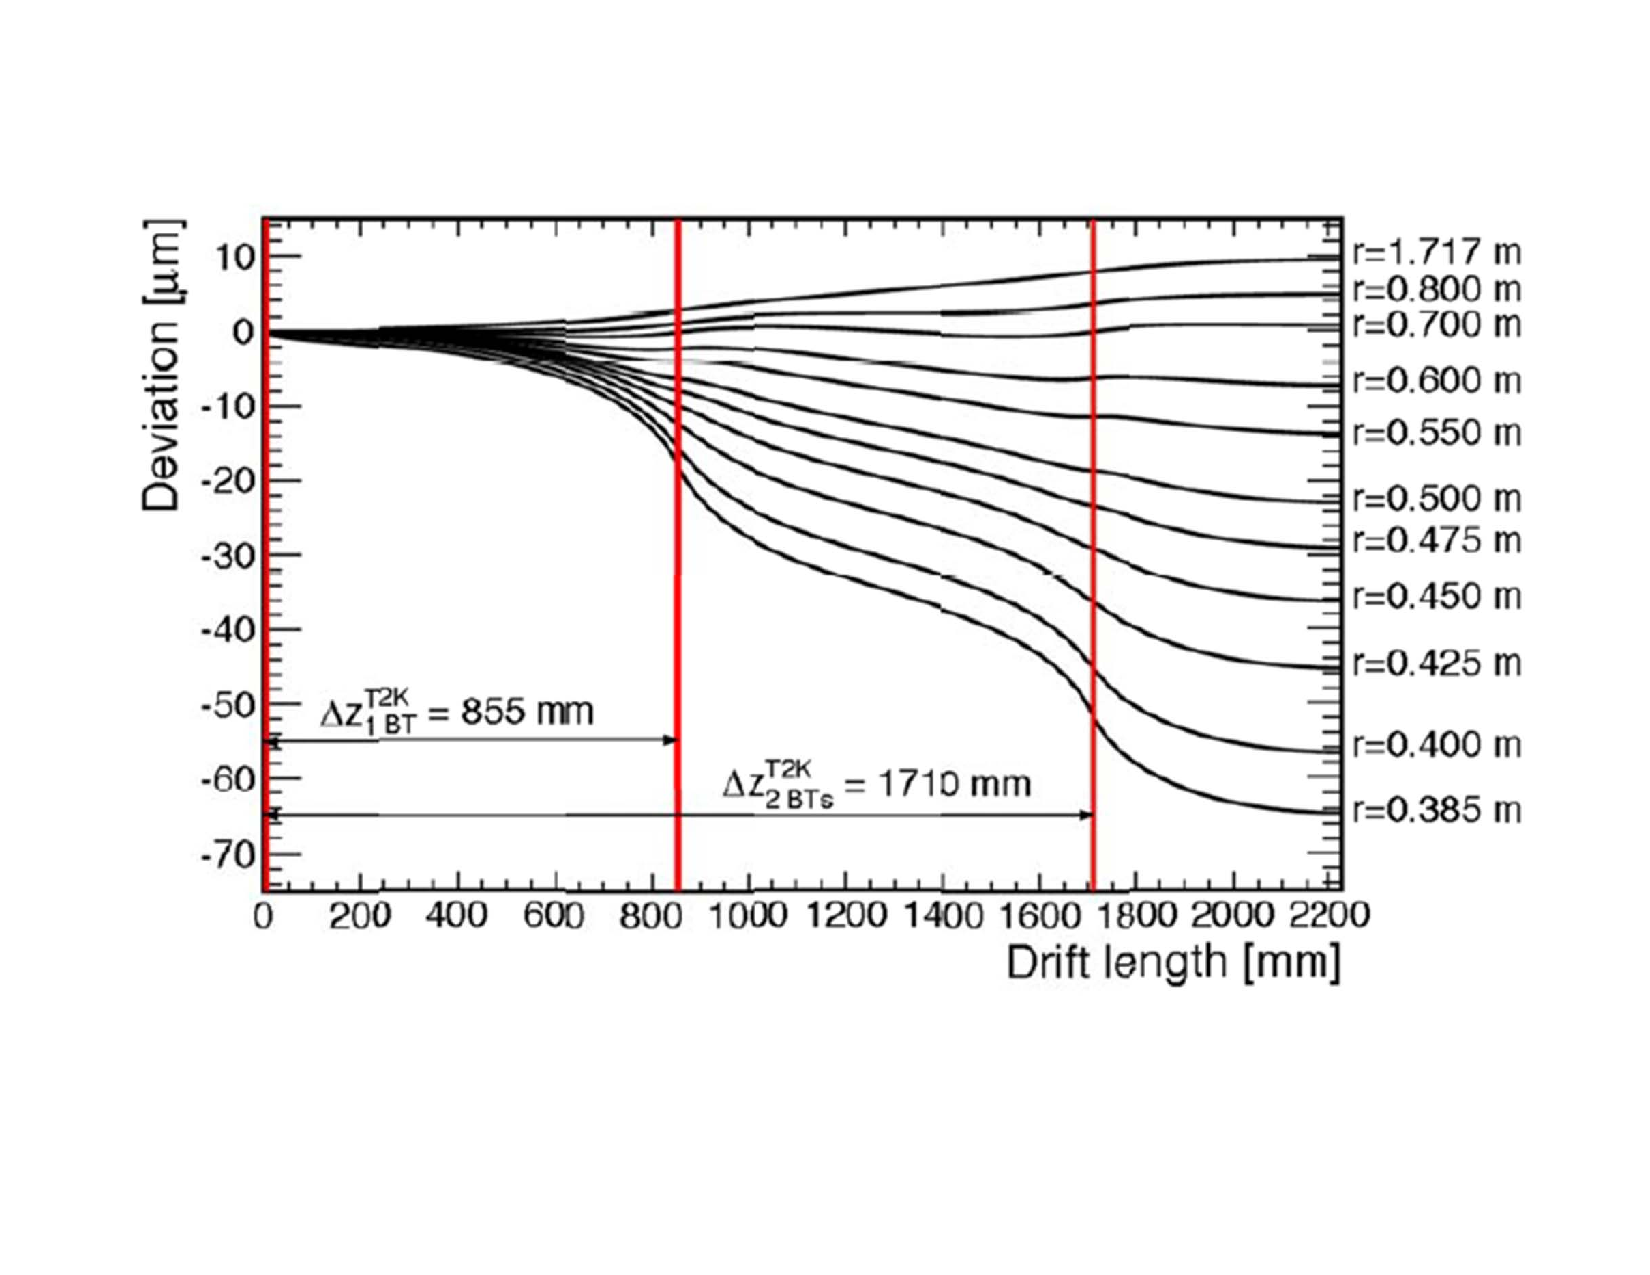
\includegraphics[width=\columnwidth]{Tracker/TPC_Bonn/plots/TPC-Gate_Fig1gating.pdf}%
\caption{\label{Fig1gating} {Displacement due to the positive-ion discs.}}
\end{center}
\end{figure}


In  Fig.~\ref{Fig1gating} it is assumed that for every drift electron one positive ion drifts back.
The actual amount of displacement should therefore be multiplied by the ratio of the gas amplification
factor to the suppression factor of the ion backflow of the MPGD system. Since the suppression factor by the
MPGD system has been measured to be in the order of order 10$^{-3}$ at
best \cite{Fujii_IonEffects}, the ratio will be larger than one for a gas gain of a few thousand, and distortions larger
than \SI{60}{\micro\meter} in some parts of TPC would be expected.

At the ILC a TPC point resolution of \SI{100}{\micro\meter} or better is required by the physics. Thus it is
necessary to either install an efficient gating device to block the ions from the gas amplification, or to correct
the track distortion. Because the machine backgrounds at ILC may not be stable enough to make a reliable
correction possible, an efficient gating device will be needed. Fortunately the bunch-train configuration of ILC
has an ideal time structure for ion gating. The positive ions drift back around \SI{5}{\milli\meter} during
the \SI{1}{\milli\second} bunch-crossing period, and can be absorbed by the ion gate which is `closed' (explanation
below) during next \SI{200}{\milli\second} between the bunch trains.

For the expected particle density at ILC, the track distortion by the
{\em{primary}} ions produced in the LCTPC volume is small and has negligible effect.



\subsubsection{Engineering Challenges: a Wire Gate or a GEM Gate}

Ion gates used for TPCs in past collider experiments consisted of a wire grid. The operation and
structure of the wire gate is well known and can be used for the LCTPC. Figure~\ref{Fig2gating} shows
a simple mechanical prototype of such a wire gate mounted on an Asian GEM module.

%Figure2Fig.2Prototype wire gate installed on the Asian GEM module

\begin{figure}[htb!]
\begin{center}
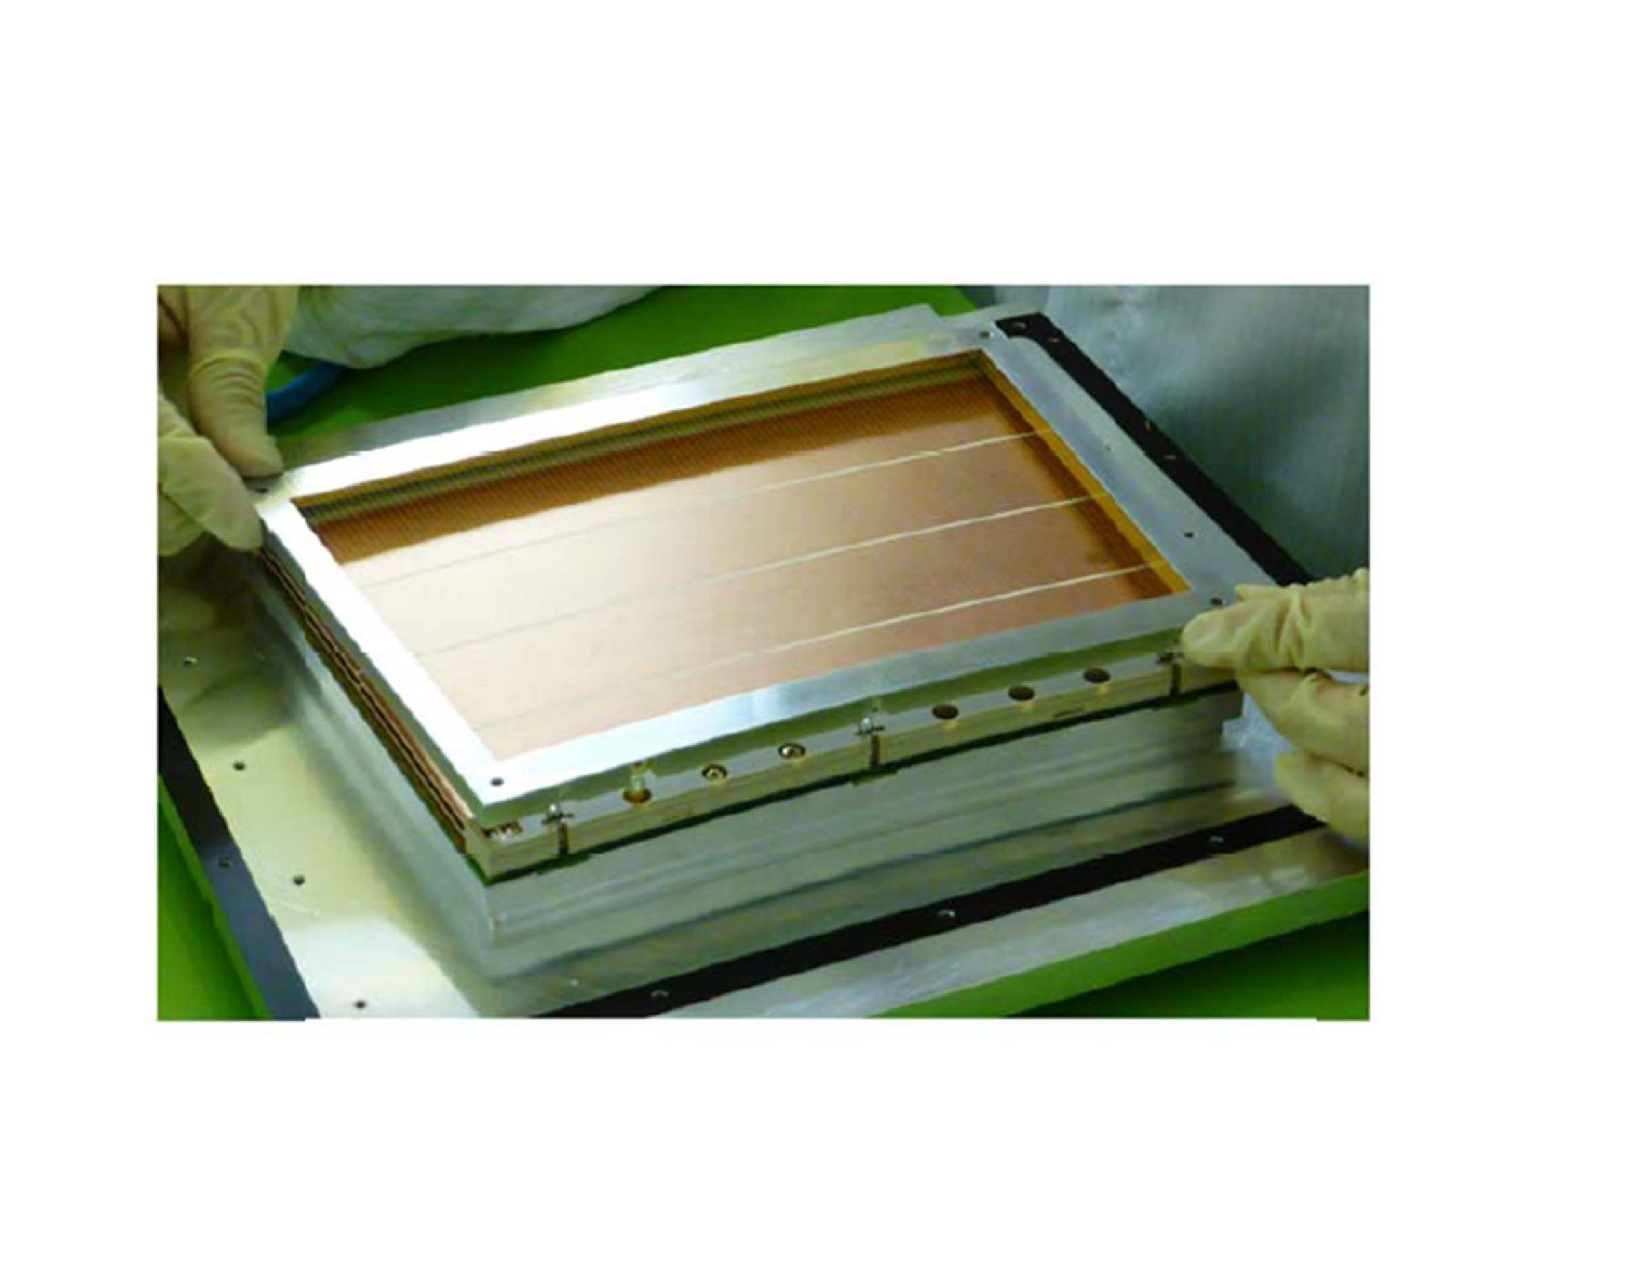
\includegraphics[width=\columnwidth]{Tracker/TPC_Bonn/plots/TPC-Gate_Fig2gating.pdf}%
\caption{\label{Fig2gating} {Prototype wire gate installed on the Asian GEM module.}}
\end{center}
\end{figure}

The disadvantage of a wire gate for the LCTPC module is to deteriorate the advantages of an MPGD TPC:
the material and space budgets are increased because of the mechanical structure needed to support the many
stretched wires on the module. Therefore, the wire gate is kept as a backup option for the LCTPC, and efforts
are focused on the development of the gate using a GEM foil.

The idea of the GEM gate was proposed by F.~Sauli in 2006 \cite{Sauli2006269}.
The ions from the gas amplification have to be absorbed by the electrode of the gate-GEM in the gate-closed condition.
`Closed' is where the electric field across the gate-GEM is reversed by changing the potential of the bottom
electrode of the gate by about \unit[10]{V}. In the gate-open condition the drift electrons need to reach
to the gas amplification region with a high efficiency in order to not deteriorate the LCTPC resolution
due to loss of signal.

Details of the simulation of GEM gate using the Garfield++ may be found in \cite{LC-DET-2012-079}. Experience was that it is easy
to stop the ions with the necessary suppression factor of 10$^{-4}$ or smaller. On the other hand, it is more
of a challenge to keep a very high efficiency of the drift electrons passing through the gate-GEM in the gate-open
condition. This is because the efficiency is limited by the optical transparency of the gate-GEM when a TPC
is used in a high magnetic field (as in the \unit[3.5]{T} field of ILD) and with a high-$\omega\tau$ gas mixture,
such as the T2K gas \cite{Behnke:2013lya,ref4T2Kgas_ishikawa,Kobayashi201137,Kobayashi2013122} foreseen for the LCTPC. In this condition the drift electron tends to follow the
magnetic field lines rather than the electric field lines, which makes the optical transparency an important parameter .

The first GEM gate prototype for the Asian GEM module for the TPC large prototype (LP) beam test at
DESY in 2009 was \unit[14]{\micro m} thick with the round GEM holes of
\unit[90]{\micro m} diameter and \unit[140]{\micro m} pitch. It had a maximum electron
transmission of 50\% in the magnetic fields of \unit[1]{T} and \unit[0]{T}. It was clear that a GEM
with bigger holes and a narrow rim was needed, that is with larger optical transparency. Simulations found that
GEM holes of the honeycomb shape with very thin rims would maximize the optical transparency.

\begin{figure}[htb!]
\begin{center}
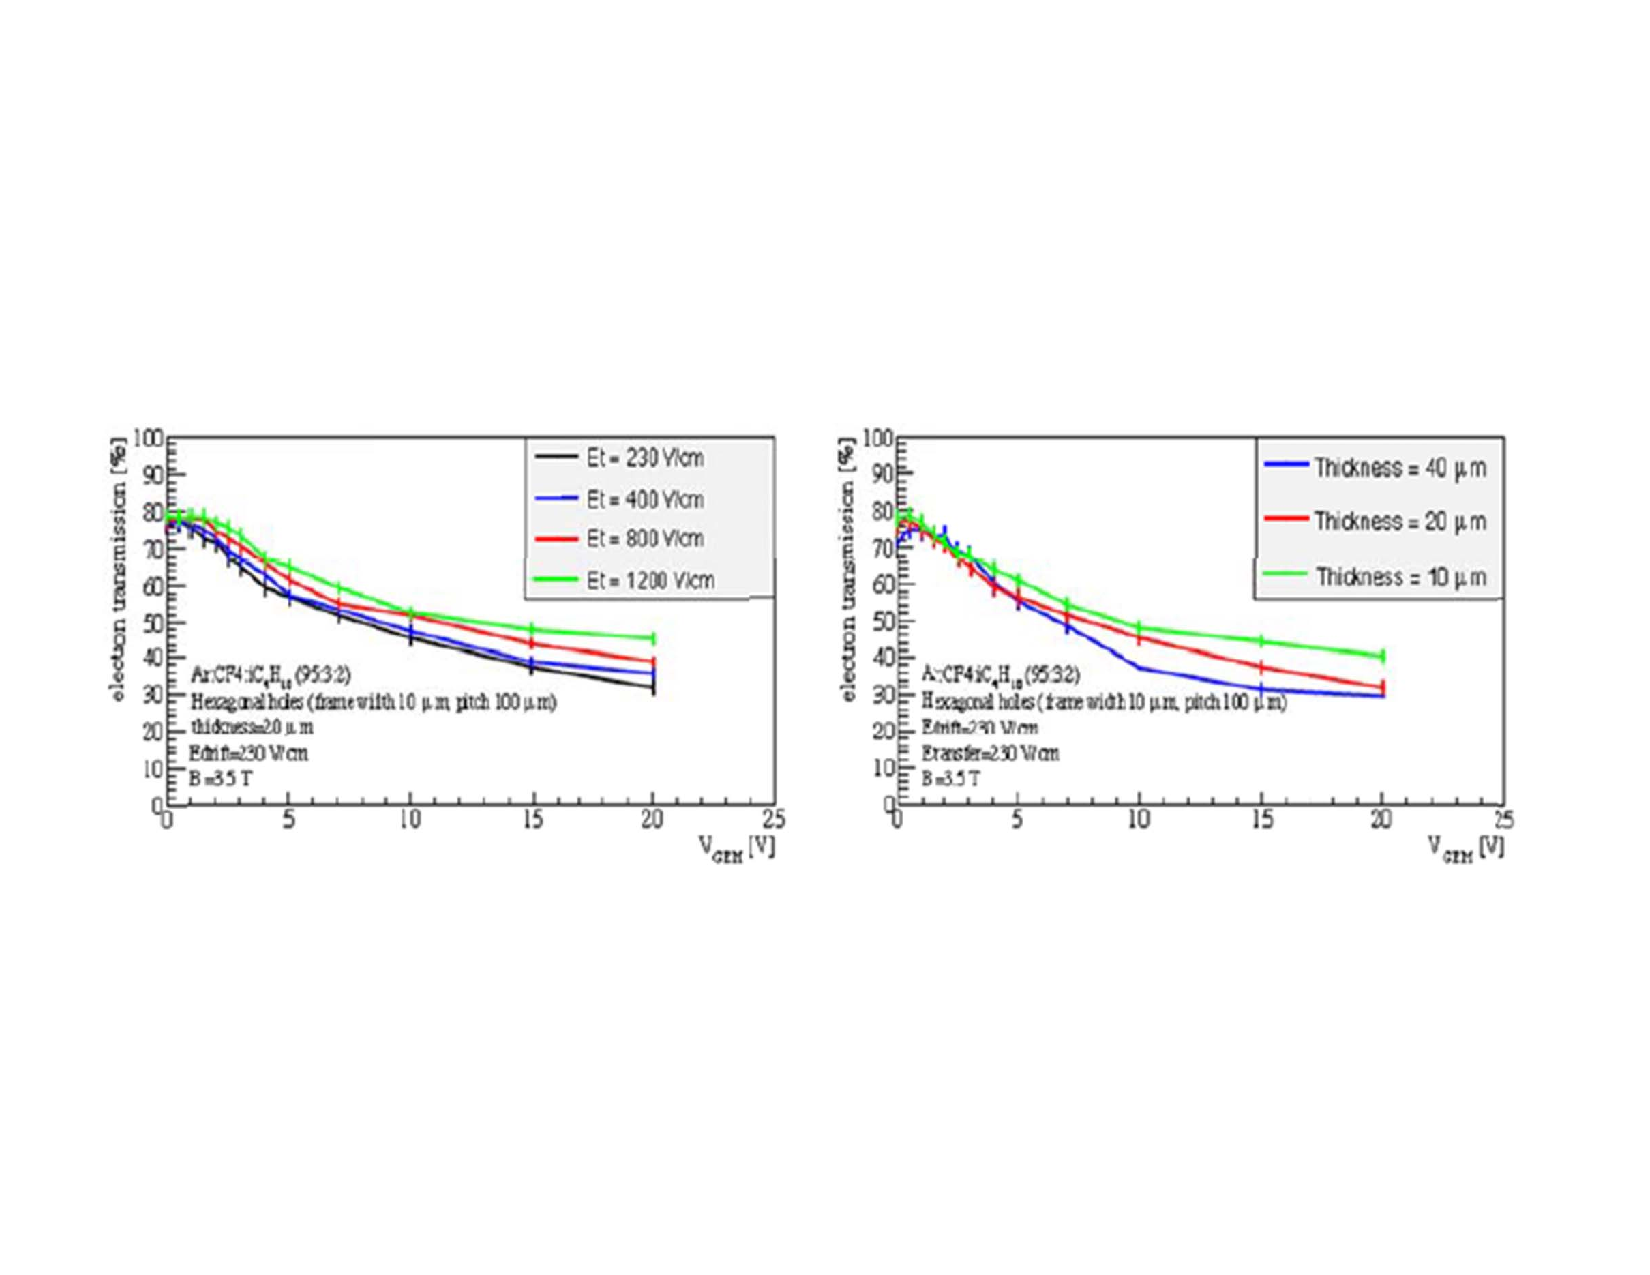
\includegraphics[width=\columnwidth]{Tracker/TPC_Bonn/plots/TPC-Gate_Fig3gating.pdf}%
\caption{\label{Fig3gating} {The electron transmission simulated for a gate-GEM with the honeycomb-shaped holes of pitch \SI{100}{\micro\meter} and rim width \SI{10}{\micro\meter}.}}
\end{center}
\end{figure}

As is seen the simulation results shown in Fig.~\ref{Fig3gating}, the thin gate GEM with
honey\-comb-shaped holes of \SI{100}{\micro\meter} pitch and \SI{10}{\micro\meter} rim width is shown to reach
an electron transmission of \SI{80}{\percent}. However, a rim width of \SI{10}{\micro\meter} turns out to be very difficult to produce;
an alternative is presented in the next subsection.

\subsubsection{Recent Milestones}

In 2013 the Japanese LCTPC group started the actual fabrication of the GEM gate with the large
optical transmission. With the limitations of the available processes of GEM, the specifications
were set using  Fig.~\ref{Fig45gating}(lower)
which are summarized in the Table 1. The target is to fabricate a gate GEM with  honeycomb shape holes
of around \SI{300}{\micro\meter} diameter and  rim-width of \SI{35}{\micro\meter} or smaller. The immediate goal
of this study is to test the Asian LP module with this GEM gate in the DESY test beam in 2016.

\begin{table}[]
\begin{center}
\begin{tabular}{|l|l|}
\hline
Item & Specification \\%$\sim$
\hline
\hline
Optical aperture ratio &  \SI{80}{\percent} \\
Hole size       & \SI{300}{\micro\meter}\\
Hole pitch       & \SI{335}{\micro\meter}\\
Rim size            & \SI{35}{\micro\meter}  \\
Insulator thickness  & \SI{25}{\micro\meter}\\
Foil size            & \SI{170x220}{\milli\meter} \\
\hline
\end{tabular}
\caption{\label{gatespecs} Specification of the gate-GEM in the current study.}
\end{center}
\end{table}

%

Prior to the fabrication of a large, module-sized gate, many small samples of
\unit{10}{cm} $\times$ \unit{10}{cm} were produced to test different processing techniques.
Although some samples by the standard single-mask chemical process were promising, limited resources required that
a major effort be continued with Fujikura Ltd.~\cite{ref5fujikuraltd} using their laser-chemical hybrid technology to produce
FPCs (flexible printed circuits). Details of the Fujikura process for the gate-GEM were presented at MPGD2015 \cite{MPGD2015_gate}.
Figure~\ref{Fig45gating}(upper) shows the structure of one of the gate-GEM small samples made by Fujikura
according to the specifications in Table \ref{gatespecs}.

%Fig. 4: Honeycomb GEM hole structure of the gate GEM. The pitch of the holes is
%335�m, the rim width 29�m. The polyimide insulator is 12.7�m thick. The thickness
%of the electrodes is given in reference (1).


%Fig. 5: Preliminary results of the electron transmission measurement are compared
%to the simulation as functions of the GEM voltage for two types of the gate GEM
%sample with larger optical transparency. In the left panel are  results for the %gate GEM
%with  round GEM holes, and in the right panel results using the gate GEM with the %honeycomb
%holes. The simulation results in the magnetic filed of 3.5T are also shown.

\begin{figure}[htb!]
\begin{center}
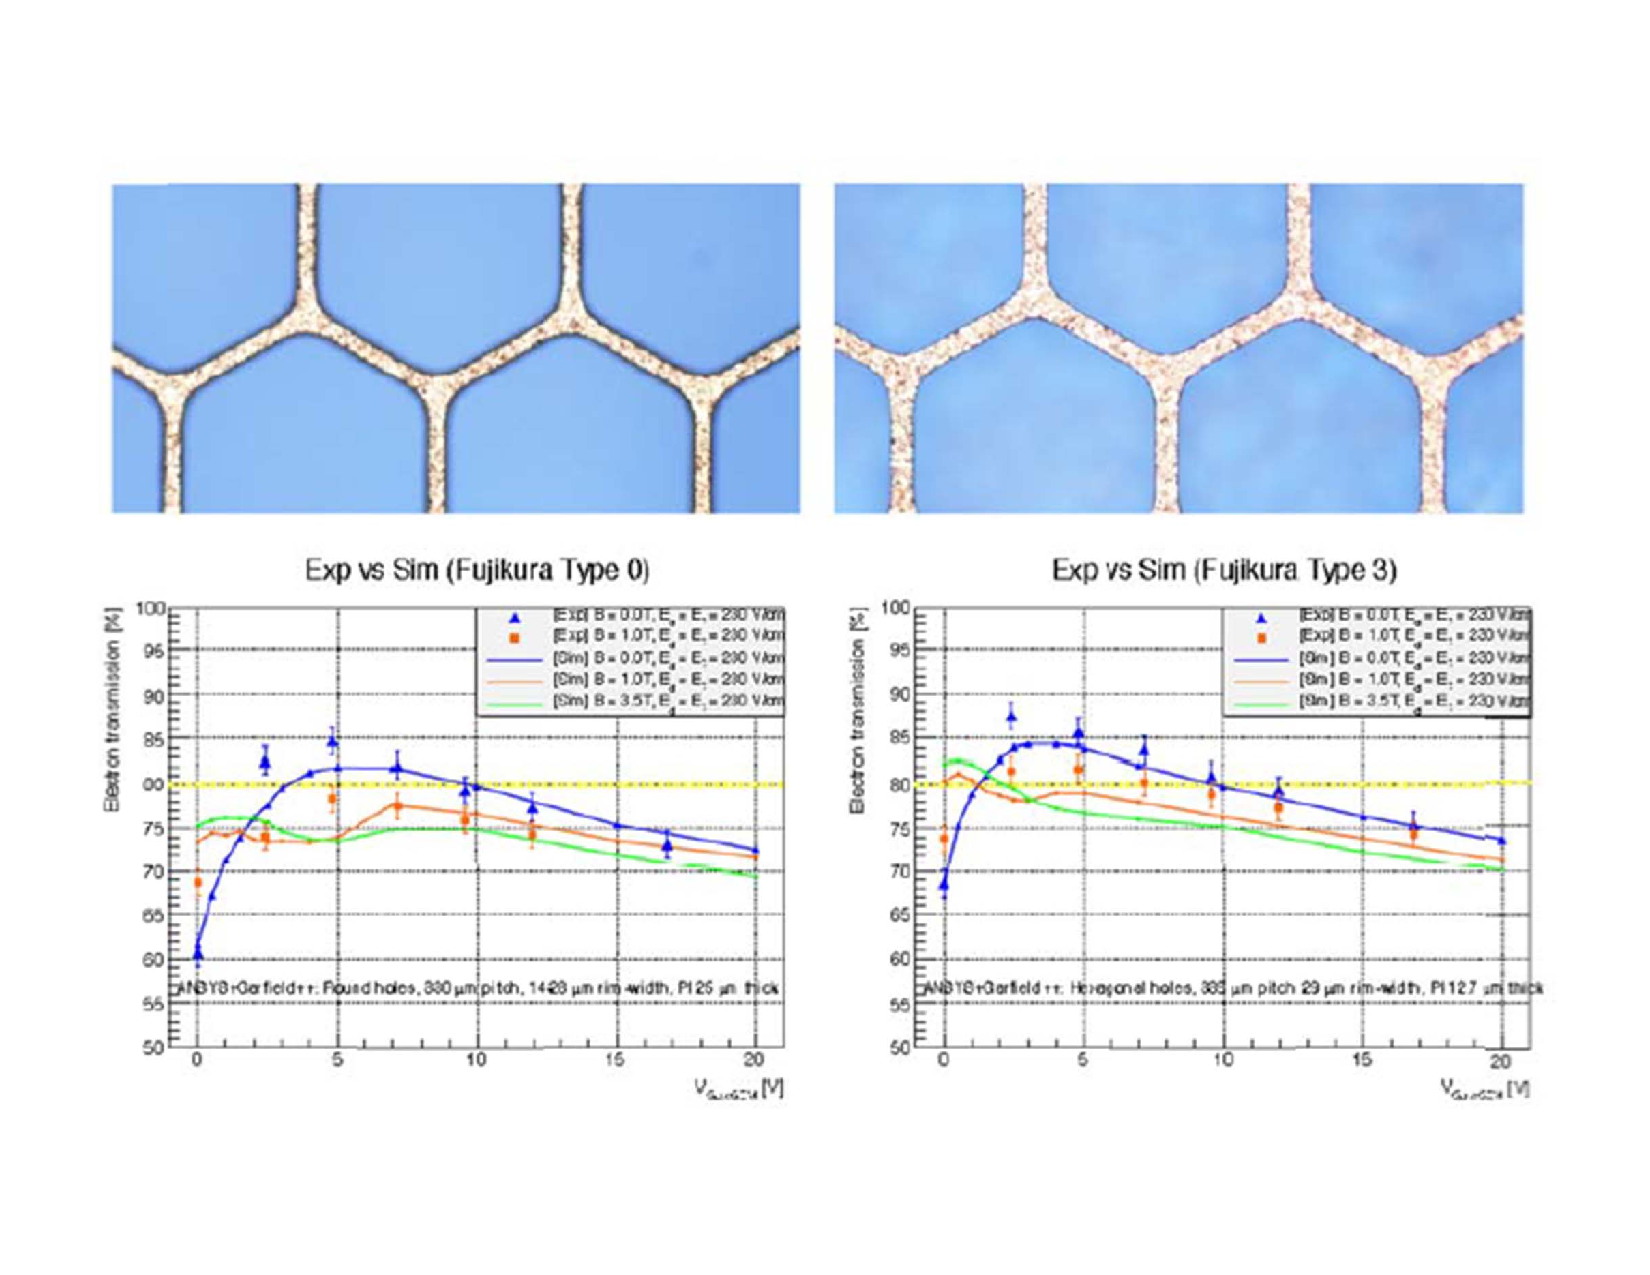
\includegraphics[width=\columnwidth]{Tracker/TPC_Bonn/plots/TPC-Gate_Fig45gating.pdf}%
\caption{\label{Fig45gating} {Upper: Honeycomb hole structure of the gate-GEM.
The pitch of the holes is \SI{335}{\micro\meter}, the rim width \SI{29}{\micro\meter}.
The polyimide insulator is \SI{12.7}{\micro\meter} thick.
Lower: Preliminary results of the electron transmission measurement are compared to simulation
as functions of the GEM voltage for two types of gate-GEMs. In the left panel are
results for gate-GEM with round holes; in the right panel results for the gate-GEM with the honeycomb-shaped holes.}}
\end{center}
\end{figure}


The electron transmission was measured for these samples, and
Fig.~\ref{Fig45gating}(lower) shows the results of the measurement compared to the simulation in magnetic fields
of 0, 1 and \SI{3.5}{\tesla}. In the left panel, the results for the sample with round holes, and in the right panel
for the sample with honeycomb-shaped holes.  The electron transmissions at 0 and \SI{1}{\tesla} were confirmed
to be better than \SI{80}{\percent} while the optical transmission was calculated to be \SI{82}{\percent} for the honeycomb-shaped-hole sample.

Having established the best configuration and the best process for the gate GEM with the small samples,
the focus has now moved to the fabrication of the gate-GEM with  the size of the Asian GEM module (Fig.~\ref{Fig6gating}).
Here the major issue for the fabrication is to minimize any defects in the electrode circuit of the gate-GEM
so that there is \SI{100}{\percent} stopping power of the ions.

%Figure 6: A sample of the gate GEM for the Asian GEM module

\begin{figure}[htb!]
\begin{center}
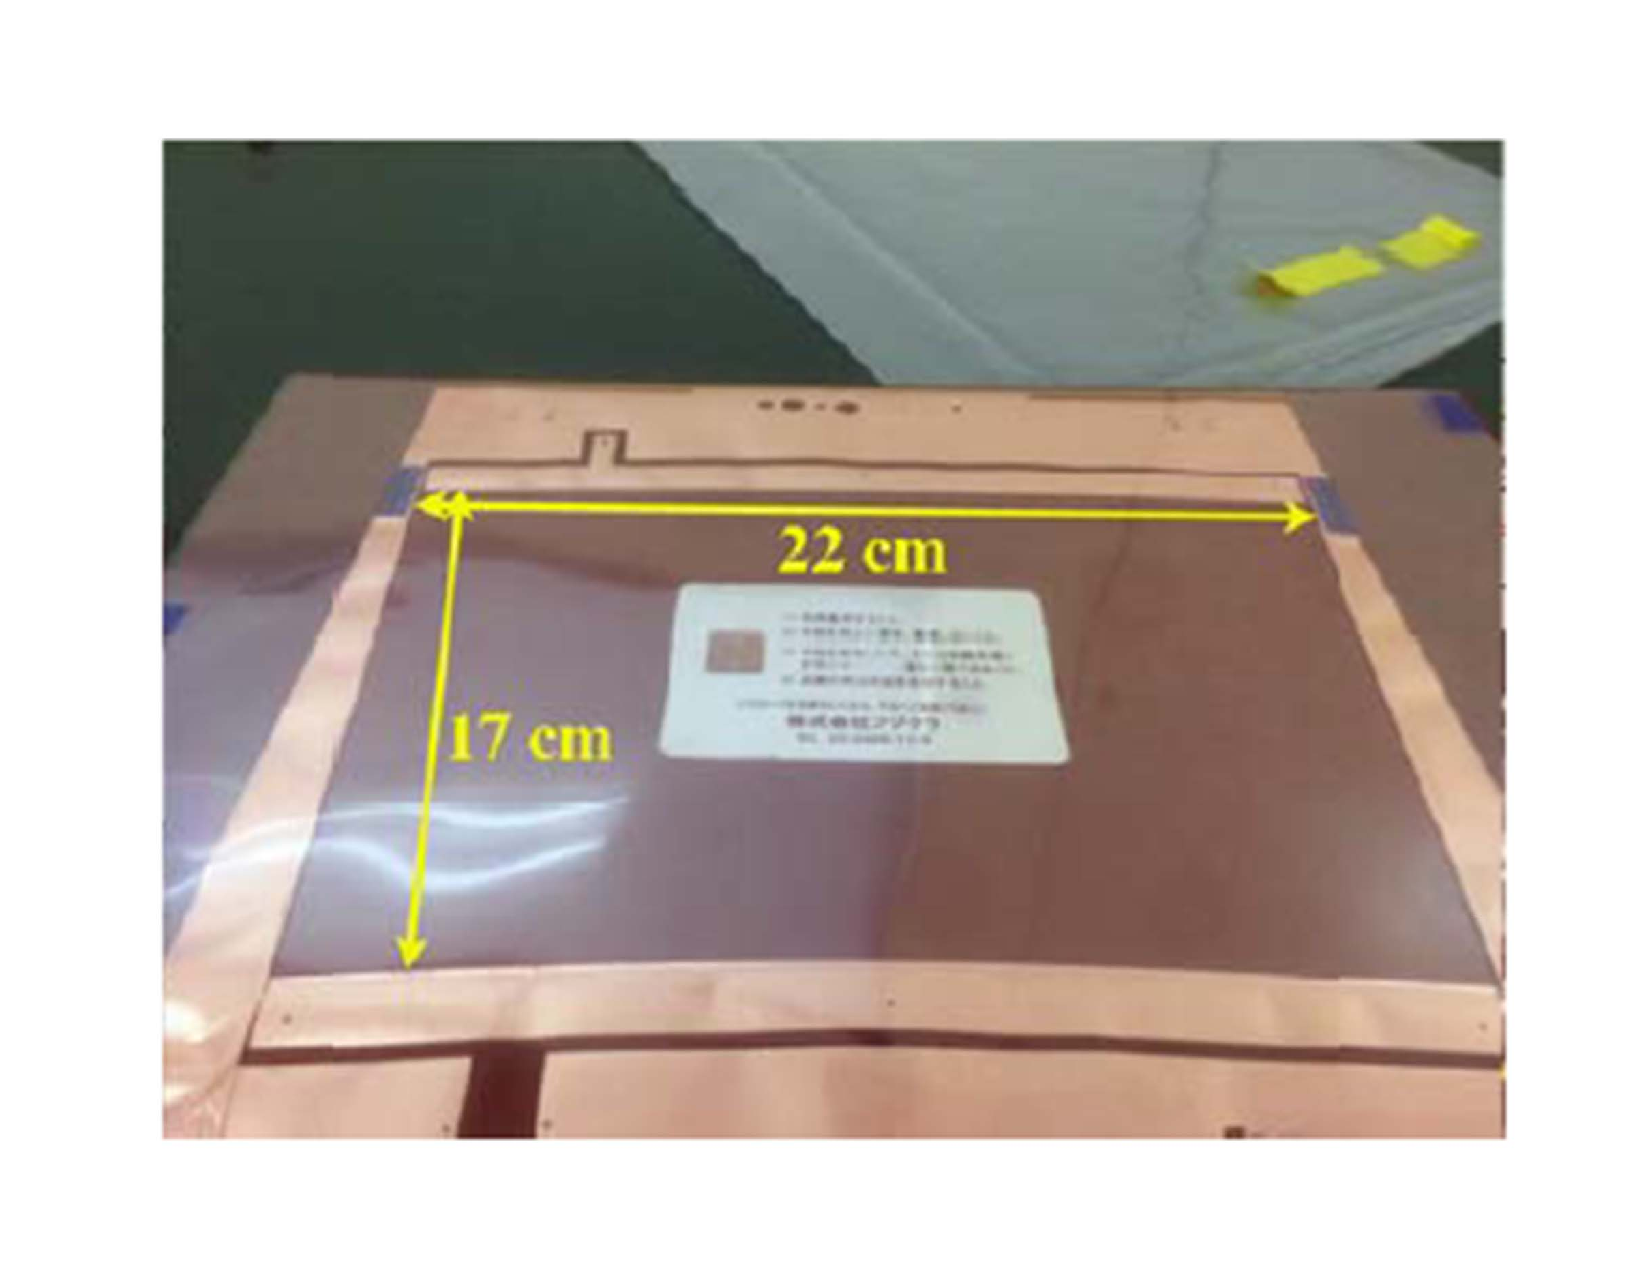
\includegraphics[width=\columnwidth]{Tracker/TPC_Bonn/plots/TPC-Gate_Fig6gating.pdf}%
\caption{\label{Fig6gating} {A sample gate-GEM for the Asian module.}}
\end{center}
\end{figure}

%Figure 7 the test mounting of the gate-GEM on the module
%Fig. 8: Test assembly of the gate GEM on the Asian GEM module

\begin{figure}[htb!]
\begin{center}
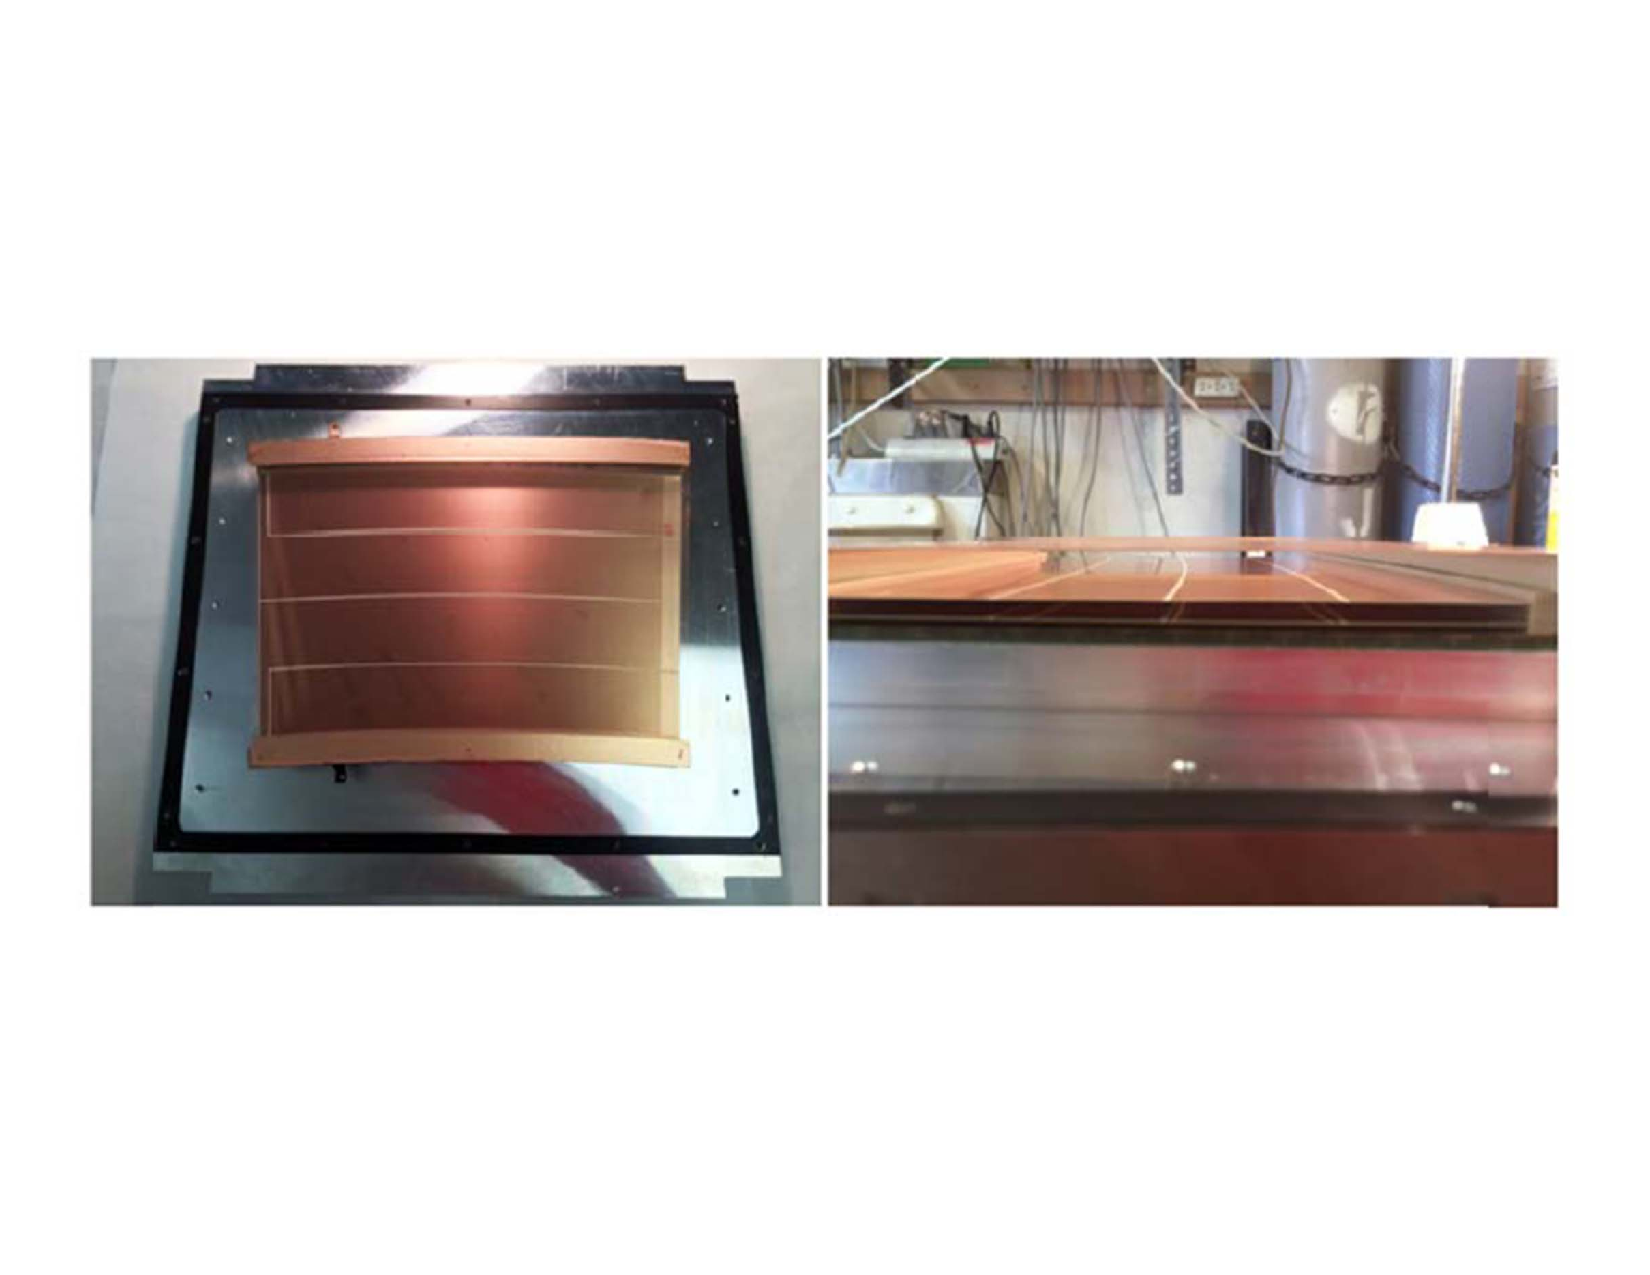
\includegraphics[width=\columnwidth]{Tracker/TPC_Bonn/plots/TPC-Gate_Fig78gating.pdf}%
\caption{\label{Fig78gating} {Left panel: Test mounting of the gate-GEM. Right panel: Test assembly of the gate GEM on the Asian GEM module.}}
\end{center}
\end{figure}

Figure~\ref{Fig78gating}(left) shows the test mounting of the gate-GEM on the module. As can be seen,
the pattern of the amplifier GEM below the thin gate-GEM can be seen clearly, indicating a  high optical transparency.
Figure~\ref{Fig78gating}(right) is a picture of a test assembly of the gate-GEM on the module.

\subsubsection{Future Plans}

The production process for the large gate-GEM has been essentially established,
and a few of the good samples for the Asian GEM module have been delivered for testing.
The preparations for measuring the electron transmission by using a laser beam are under way.
Although the Asian model is designed to have a GEM gate mounted on it,
there may be more issues coming up, and some optimization of the mounting method and the module structure
might become necessary for the design of the LCTPC. Beside some difficulties to stretch such a thin
GEM stably, some consideration on the possible ion leak through the module boundaries
for the Asian GEM modules may be needed.

\subsection{Electronics, DAQ and Cooling}\label{chap:TPC_sec:electronics}
Contact person: Leif J{\"o}nsson (email: leif.jonsson@hep.lu.se)\\

\subsubsection{Introduction}
The readout electronics for the TPC has to be adapted to the design of the tracking chamber and the beam structure of the collider. The physics goals of the ILC requires high momentum resolution and two-track separation, which drive the track reconstruction in the $r\text{-}\varphi$-plane to pad sizes of small dimensions. For the $r\text{-}z$-plane a short shaping time and a high sampling rate is necessary to provide the best possible timing information. However, at the same time the noise level has to be kept at a manageable level. The sampling depth has to match the sampling frequency in order to cover the full drift length. The front end electronics has to be accommodated within pad modules, with a channel occupancy that is smaller than the pad size to allow space for the mounting frame, the voltage supply and the cooling system.

The power consumption of the front-end electronics should be kept low such that the heat dissipation does not lead to a temperature increase in the TPC-gas of more than typically \unit[1]{\textdegree C} and in order to minimize the cooling requirements. In this respect, power pulsing, where the front-end electronics is switched off for about \unit[199]{ms} between the bunch trains, helps significantly.

The readout electronics presently under development aims to demonstrate that the channel occupancy can be made compatible with the small pad size foreseen. It is based on the CERN SALTRO16-chip, which integrates the analogue and digital signal processing of the incoming signals within the same compact circuit. The size of the chip itself is $8.7 \times \unit[6.2]{mm^2}$ and it contains 16 readout channels. The chip is programmable with respect to gain, rise time, decay time and polarity. The sampling can be clocked at frequencies 5, 10, 20 and \unit[40]{MHz} and it allows for power pulsing.

\noindent The chips are bonded onto carrier boards of size $12.0 \times \unit[8.9]{mm^2}$, also offering space for passive components along the edges. Each board contains more than 200 bonding wires, which considering the small size of the board requires a very accurate bonding procedure. The upper surface is covered by an epoxy glob protecting the chip, the bonding wires and the passive components. The bottom side contains small tin balls organized in a BGA pattern for soldering of the carrier board on so called Multi-Chip Modules (MCM).

\noindent Eight carrier boards are mounted on an MCM, which also contains a CPLD (Complex Programmable Logic Device) controlling the data flow. The MCM-board is the smallest unit in the front end electronics and it is attached to the pad plane via four micro-connectors, whereas on the opposite side of the board there are two connectors, via which the low voltage is distributed and the signals are transmitted. The MCM-board is designed in High Density Interconnect (HDI) technology, by which the number of layers is significantly reduced compared to conventional PCB design. The dimensions of the MCM-board are $32.5 \times \unit[25]{mm^2}$ and serves 128 readout channels. This corresponds to a channel occupancy of about $\unit{6.4}{mm^{2}}$, although some space is also required for the high voltage connectors of the gas amplification system (GEMs and Micromegas) and the cooling system.

\noindent A serial readout system is used for the signal transfer to the DAQ computer. The MCM-board and the Scalable Readout Unit (SRU) communicate directly via the Data Trigger Control (DTC) link. Communication, data transfer and control, between the SRU and a DAQ computer is done via Ethernet.

\noindent Cooling of the front end electronics is a challenge since the size of the cooling system must match the smallness of the electronics and still provide efficient cooling. The total power consumption of an MCM-board in continuous operation
is \unit[3203]{mW} on the top side and \unit[3028]{mW} on the bottom side. In power pulsing mode, with a bunch train of \unit[725]{\micro s}, containing 1312 bunches, the power dissipation is reduced to about \unit[223]{mW} per MCM-board on the top side and \unit[48]{mW} on the bottom side. A cooling system with cooling pipes that run on top of the MCM-boards, using two-phase \ce{CO2} coolant, is considered. Another possibility would be to use micro-channel cooling, which has been developed by the semiconductor community. Such systems are presently further developed within the AIDA2020 project, for applications in high energy physics experiments. The ILC cycle is not realistic in a test beam environment as at e.g. DESY. To get a reasonable trigger rate is e.g. a cycle with \unit[5]{ms} beam at \unit[10]{Hz} more useful, which corresponds to \unit[343]{mW} per MCM-board on the top side and \unit[168]{mW} on the bottom side, in power pulsing mode.

\subsubsection{Recent Milestones}
A test system has been built and a few mounted carrier boards have been produced, which are both under debugging. The design of the MCM-board in HDI-technology is ready and the production is awaiting the full characterisation of the carrier board. The design of the low voltage board is essentially ready. An MCM-development board, containing only one packaged SALTRO-chip, has been produced and has been used in the tests of the serial readout system. The tests were successful, although some further firmware development is needed for the full functionality. A cooling system using micro-channel cooling is under discussion within AIDA2020.

\subsubsection{Engineering Challenges}
The final aim is to produce front end electronics, high voltage supply and a cooling system which are compatible with a pad size of $1 \times \unit[6]{mm^2}$. The compactness of the electronics and the space limitations are major challenges, as well as designing a suitable and efficient cooling system. An elegant solution for the low voltage supply has to be found and due to space limitations the design of the mechanical support for the electronics is also a challenge.

\subsubsection{Future Plans}
In the next future the characterisation of the carrier board will be completed, followed by the production of the MCM-board. One fully mounted MCM-board with eight carrier boards will be produced and tested. The firmware for the serial readout will be further developed and tested. Discussions concerning micro-channel cooling will continue and we hope to get help with the design and production of a prototype system by AIDA2020.

\subsubsection{Applications Outside of Linear Colliders}
The front end electronics, based on the SALTRO16-chip provides a very versatile system in the sense that it offers the possibility to set various readout parameters (polarity, shaping time, gain, decay time) in the SALTRO pre-amplifier. It is optimised for low capacitance detectors, sensitive to femtocoulomb signals with digital correction of the base line, followed by advanced pulse recognition and zero suppression.  In that sense the SALTRO-chip can be regarded as a highly sensitive 16 channel digital oscilloscope. The small units of the readout system are suitable for applications and detector R\&D in a variety of other fields like medical diagnostics, material science at XFEL, and for investigations at ESS.

\subsection{Mechanics and Calibration}\label{chap:TPC_sec:mechanics}
Contact person: Ties Behnke (email: ties.behnke\@ desy.de)\\

\subsubsection{Introduction}
A key component of the TPC at a future collider will be the design and construction of the field cage. The cage should be light weight, yet mechanically and electrically stable. It should provide support for the cathode and the anode systems, and allow excellent field shaping in between.
To test the concept for such a field cage a prototype has been built as part of the LCTPC test infrastructure \cite{1748-0221-5-10-P10011}. The field cage is made from a light weight composite sandwich structure. The mechanical structure is given by a honeycomb layer, which is covered on the inside and the outside by a glass fibre reinforced epoxy layer. On the inside a Kapton foil provides electrical insulation, and field shaping through a system of copper ring electrodes. On the outside a thin aluminum layer provides grounding. Integrated into the field cage a laser based calibration system is foreseen.

The prototype field cage has been constructed in 2008 and has been used with all different readout technologies since. It is equipped with an aluminum based endplate, which can host up to seven identical readout modules. It is designed to fit into the PCMAG magnet \cite{Yamamoto199475} infrastructure, which is installed at the DESY test beam facility \cite{DESY2TB}.

%Another challenge is the development of a compact and efficient cooling strategy. Currently, CO$_2$ based systems are favoured and are being prototyped.

A large system like the TPC poses particular challenges to calibrate the system and to maintain the calibration. Currently several systems are under consideration.

An important part of the calibration will be done based on data recorded, without special hardware. Tracks will be used to align the different modules relative to each other, and to measure and correct field distortions.

While tracks are an excellent method to derive relative corrections, and to equalise the response, it might be difficult to reach the ultimate absolute resolution without an external unbiased reference. This reference can come from different sources. Within the ILD detector design silicon detectors are foreseen before and after the TPC, which will provide an external reference. These systems can be used to calibrate the field distortions, and to set the scale for the momentum measurement. Another system will be based on laser beams. Laser beams will be used in two ways. Well focused small cross section beams can be inserted into the drift volume, and serve as fake tracks. The ionization along the laser beams is recorded as for normal tracks, and can be used to calibrate the response of the TPC. A wide laser beam can be used to illuminate the cathode of the TPC. Dots or lines of a low work-function material like e.g.~aluminium on the surface of the cathode would then provide well defined spots where the laser
light can liberate electrons. These electrons then drift towards the anode and sample any inhomogeneities on their way. Thus, they can be used to monitor and ---to some extent--- determine the field properties inside the drift volume. Both types of laser beams need to be inserted into the TPC, and will require the design and implementation of sophisticated hardware.

% %\subsection{Recent Milestones}
\subsubsection{Engineering Challenges}
The current field cage has been successfully used in numerous test beam campaigns. However, it has failed to deliver the ultimate mechanical precision which is needed for the demonstration of the anticipated momentum resolution of the TPC system. In particular, the manufacturer has failed to deliver the needed alignment between the anode and the cathode, and has introduced a small overall skew into the field cage. The main challenge will be to develop and build a second generation field cage which fulfills the precision requirements. For this an entirely new tooling is being developed, which should help to ensure the mechanical precision.

The results from this prototype field cage will then be applied to a study of the design of the full field cage for the ILD TPC. A central and so far unsolved engineering challenge is the support of the TPC in the overall detector. Here a combination of light weight, space saving support structures combined with superb mechanical stiffness need to be found. Particular attention will also need to be payed to the behaviour of the system in case of earth quakes, given that the proposed site of the ILC in Japan is located in an earth-quake prone region.

An open and as yet unsolved issue is the design of the central cathode of the TPC. This system is located in the centre of the detector, very difficult to access. It needs to be light weight, yet dimensionally very stable. It will be supplied with high voltage of close to \unit[100]{kV}. The supply of this very high potential in a safe and reliable way is under study and represents significant challenges.

As described above laser beams will be used to calibrate the system. The insertion and guidance of these laser beams present significant challenges. Ways will need to be found to bring the laser beams to the TPC. The laser will have to be installed on the outside of the detector, so that transport ways of several meters through a very crowded environment are needed.

\subsubsection{Future Plans}
Over the next few years a full engineering design of the ILD TPC will be developed. This will include a detailed simulation of the TPC system, and its mechanical properties, and its integration into the ILD detector as a whole.

Detailed problems which will need to be addressed are:

\begin{itemize}
\item Finite Element Method (FEM) calculations of the field cage and the endplate
\item Optimisation and final decision on the layout of the endplate: size of modules, number of modules, etc.
\item Design of the support system of the TPC in the ILD detector
\item Study of the mechanical properties of the TPC support in view of vibrations and overall stability
\item Design and implementation of a system of laser beams in the TPC drift volume
\item Design and implementation of a system to illuminate the TPC cathode with a laser beam.
\end{itemize}

%Contributing : DESY, KEK, U Cornell, U Hamburg, CEA Saclay, Nikhef, U Victoria

%\subsection{Recent Milestones}

%The cooling system of the PCMAG has been modified from cooling with liquid helium to a system using a closed helium circuit with external compressors and cold heads installed in the PCMAG. This allows a continuous operation over long time periods of several months and improves the usability and safety of the setup.

%Contributing: AIDA, KEK, DESY

%A two-phase CO$_2$ cooling system (TRACI) has been installed at the test beam area and successfully operated at two test beam periods, so far.

%Contributing: KEK, DESY, Nikhef, CEA Saclay
%
%
%\subsection{Engineering Challenges}
%
%The field cage of the LPTPC has to be mechanically and electrically stable, while keeping the material budget of its wall structure at about 1\% of X$_0$. Its mechanical tolerances are very tight to ensure an electric field homogeneity of $10^{-4}$.
%
%\subsection{Future Plans}
%
%The first field cage of the LPTPC had been designed at DESY and built by an external company.  The allowed mechanical tolerance of max. $0.5\,\mathrm{mm}$ for the tilt of the cylinder axis was not kept. A new field cage will be constructed in-house at DESY. Material tests and the preparation of the required construction tools are ongoing.

\thispagestyle{empty}
\newgeometry{margin=1.5cm} % modify this if you need even more space
\begin{landscape}
    \centering
    \begin{adjustbox}{max width=1\textwidth,totalheight=1\textheight}
\begin{tabularx}{\textheight}{lXXXX}
    \toprule
    R\&D Technology & Participating Institutes & Description / Concept & Milestones & Future Activities \\
    \midrule
    \bottomrule
\end{tabularx}
\end{adjustbox}
\end{landscape}
\restoregeometry



\begin{thebibliography}{9}



%%%%% Section 1 Introduction    %%%%%%%%%%%%%%%%%%
% \bibitem{TESLA-CDR}$e^+ e^-$ Linear Collider Physics and Detector Studies, Part E,
% Edited by R.~Settles, DESY 97-123E (December 1997) p 541





%%%%% GEM Introduction %%%%%%%%%%%%%%%%%

% \bibitem{Sauli_GEM}
% F.~Sauli, \textit{``{GEM: A new concept for electron amplification in gas detectors}''},
%   \url{http://dx.doi.org/10.1016/S0168-9002(96)01172-2}, {\textbf{ {Nucl.~Instr.~and Meth.~A} {\bfseries 386} (Feb,
%   1997) 531 -- 534}}.



%%%%% CHAPTER 2 Asian GEMs      %%%%%%%%%%%%%%%%%%









%%%%% Section 3 Standard GEMs   %%%%%%%%%%%%%%%%%%

% \bibitem{HallermannPhD}
% L.~Hallermann, {\textit{Analysis of GEM Properties and Development of a GEM
%   Support Structure for the ILD Time Projection Chamber}}.
% \newblock PhD thesis, {Universit\"at Hamburg}, 2010.
% \newblock
%   \url{http://www-library.desy.de/cgi-bin/showprep.pl?desy-thesis-10-015}.
% \newblock {DESY-THESIS-10-015}.

% \bibitem{DESYGEM}
% R.~Diener, T.~Behnke, S.~Caiazza, I.~Heinze, V.~{Prahl}, C.~Rosemann,
%   O.~Sch{\"a}fer, J.~Timmermans, R.~{Volkenborn}, and K.~Zenker, \textit{``{Beam Test
%   with a GridGEM TPC Prototype Module}''}, {\textbf arXiv e-prints} (Feb, 2012) ,
%   \url{http://arxiv.org/abs/1202.6510}, {{\ttfamily arXiv:1202.6510
%   [physics.ins-det]}}.
%

% \bibitem{millepedeNIM}
% V.~Blobel, \textit{``{Software alignment for tracking detectors}''},
%   \url{http://dx.doi.org/10.1016/j.nima.2006.05.157}, {{\textbf {Nucl.~Instr.~and Meth.~A {\bfseries 566} (Oct., 2006) 5--13}}}.
%

% \bibitem{millepedeWiki}
% ``{Millepede II wiki page}.''
%   \url{https://www.wiki.terascale.de/index.php/Millepede_II}.


% \bibitem{ZenkerPhD}
% K.~Zenker, {\textit {Studies of field distortions in a Time Projection Chamber for
%   the International Linear Collider}}.
% \newblock PhD thesis, {University of Hamburg}, 2014.
% \newblock
%   \url{http://www-library.desy.de/cgi-bin/showprep.pl?desy-thesis-14-044}.
% \newblock {DESY-THESIS-14-044}.
%%%%% Section 4 Micromegas %%%%%%%%%%%%%%%%%%
% \bibitem{arog09}D.~C.~Arogancia, et al., \textit{``Study in a beam test of the resolution of a Micromegas TPC with standard readout pads''}, \textbf{Nucl.~Instr.~and Meth.~A 602 (2009) 403-414}.

% \bibitem{dixit}M.~S.~Dixit, et al., \textit{``Position sensing from charge dispersion in micro-pattern gas detectors with a resistive anode''}, \textbf{Nucl.~Instr.~and Meth.~A 518 (2004) 721}.

% \bibitem{fivetesla}M.~S.~Dixit et al., \textit{``Micromegas TPC studies at high magnetic fields using the charge dispersion signal''}, \textbf{Nucl.~Instr.~and Meth.~A 581 (2007) 254-257}.

% \bibitem{t2kelec}D.~Atti{\'e} et al., \textit{``The readout electronics of the micromegas-based large time projection chamber prototype for the International Linear Collider''} (Jun 2012) DOI: 10.1109/RTC.2012.6418152

% \bibitem{bulk}I.~Giomataris, et al., \textit{``Micromegas in a bulk''}, \textbf{Nucl.~Instr.~and Meth.~A 560 (2006) 405-408}.

% \bibitem{tpcconf}I.~G.~Irastorza, P.~Colas, I.~Giomataris, Journal of Physics: Conference Series, \textit{``Sixth Symposium for Low Energy Rare Event Detection''}, \textbf{Vol. 460 (2013) Paris}.
%

%%%%% Section 5 Pixelized Readout  %%%%%%%%%%%%%%%%%%

% \bibitem{TPC_pixel_Timepix} X.~Llopart, et al., \textit{``Timepix, a 65k
%   programmable pixel readout chip for arrival time, energy and/or photon
%   counting measurements''}, \textbf{Nucl.~Instr.~and Meth.~A 581 (2007) 485-494}.

% \bibitem{TPC_pixel_GEM_TP_1} A.~Bamberger, et al., \textit{``Readout of GEM Detectors Using the Medipix2 CMOS Pixel Chip.''}, \textbf{Nucl.~Instr.~and Meth.~A 573 (2007) 361-370}.


% \bibitem{TPC_pixel_GEM_TP_2} C.~Brezina, et al., \textit{``Operation of a GEM-TPC with pixel readout''}, \textbf{IEEE TNS, Vol. 59, No. 6, December 2012, pp. 3221-3228}.
%


% \bibitem{TPC_pixel_InGrid} M.~Chefdeville, et al., \textit{``An electron-multiplying Micromegas grid made in silicon wafer post-processing technology``}, \textbf{Nucl.~Instr.~and Meth.~A 556 (2006) 490}.



% \bibitem{TPC_pixel_InGrid_prod} W.~Koppert, et al., \textit{``GridPix detectors: Production and beam test results``}, \textbf{Nucl.~Instr.~and Meth.~A 732 (2013) 245-249}.



% \bibitem{TPC_pixel_1LPmodule}
% M.~Lupberger, et al., \textit{``The Pixel-TPC: first results from an 8-InGrid module''}, {{\textbf {Journal of Instrumentation {\bfseries 9} no.~01, (2014) {C01033}}}}.




%%%%% Section 6 Gating %%%%%%%%%%%%%%%%%%



%ref1D.Arai,T.Krautscheid : Nota-this is still not quite correct

% \bibitem{LCTPCJap-IonGate}
% LCTPC~Japan~Collaboration, \textit{``Considerations for an ion gate for LCTPC''},
% \url{http://www-flc.desy.de/lcnotes/notes/LC-DET-2012-079.pdf. LC-DET-2012-079}.
%

%
% \bibitem{Fujii_IonEffects}
% K.~Fujii, \textit{``Positive Ion Effects (LCTPC collaboration meeting presentation)''},
% \url{http://agenda.linearcollider.org/event/5504/session/8/contribution/3/material/slides/0.pdf}





%ref2mpgdionsuppressionfactor  and

% \bibitem{Sauli2006_gate}
% F.~Sauli, L.~Ropelewski, P.~Everaerts, \textbf{Nucl. Instrum. and Meth. A 560 (2006)  269-277}.
%


% \bibitem{ref4T2Kgas_tdr}
% \url{https://www.linearcollider.org/ILC/Publications/Technical-Design-Report}
% The International Linear Collider, Technical Design Report, ISBN 978-3-935702-74-4,
% Volume 4.~Detectors, p.~211
%


% \bibitem{ref4T2Kgas_ishikawa}
% A.~Ishikawa et al., \textit{``Gas-Property Study at Saga U.''}, \url{http://www-hep.phys.saga-u.ac.jp/ILC-TPC/gas/index.html}
%


% \bibitem{ref4T2Kgas_kobayashi}
% M.~Kobayashi et al., \textit{``Cosmic ray tests of a GEM-based TPC prototype operated in Ar-CF4-isobutane gas mixtures''}, \textbf{Nucl.~Instr.~and Meth.~A 641 (2011) 37-47}, arXiv:1008.5068v2
%


% \bibitem{ref5fujikuraltd}
% Fujikura Ltd., Japan: \url{http://www.fujikura.co.jp/eng/}
%


% \bibitem{MPGD2015_gate}
% D.~Arai (Fujikura Ltd.), K.~Ikematsu (Saga Uni.), A.~Sugiyama (Saga Uni.), M.~Iwamura, A.~Koto, K.~Katsuki (Fujikura Ltd. ), K.~Fujii, T.~Matsuda (KEK/IPNS), MPGD2015 Trieste, 2015/10/13







%%%%% Section 7 Electronics %%%%%%%%%%%%%%%%%%









%%%%% Section 8 Mechanics %%%%%%%%%%%%%%%%%%

% \bibitem{Schade}
% T.~Behnke, K.~Dehmelt, R.~Diener, L.~Steder, T.~Matsuda, V.~Prahl, and
%   P.~Schade, \textit{``A lightweight field cage for a large {TPC} prototype for the
%   {ILC}''}, \url{http://dx.doi.org/10.1088/1748-0221/5/10/P10011}, {{\textbf {Journal
%   of Instrumentation {\bfseries 5} no.~10, (2010) {P10011}}}}.
%

% \bibitem{pcmag:magnet}
% A.~Yamamoto, K.~Anraku, R.~Golden, T.~Haga, Y.~{Higashi}, M.~Imori, S.~Inaba,
%   B.~Kimbell, N.~{Kimura}, and Y.~Makida, \textit{``{Balloon-borne experiment with a
%   superconducting solenoidal magnet spectrometer}''},
%   \url{http://dx.doi.org/10.1016/0273-1177(94)90071-X}, {{\textbf {Advances in Space
%   Research {\bfseries 14} (Feb, 1994) 2}}}.
%
%
% \bibitem{DESY2TB}
% ``{Homepage of the DESY II testbeam Facility}.'' \url{http://testbeam.desy.de}.
% %%%%% Section 9 Software %%%%%%%%%%%%%%%%%%







\end{thebibliography}

\end{document}

\thispagestyle{empty}
\newgeometry{margin=1.5cm} % modify this if you need even more space
\begin{landscape}
    \centering
    \begin{adjustbox}{max width=1\textwidth,totalheight=1\textheight}
\begin{tabularx}{\textheight}{lXXXX}
    \toprule
    R\&D Technology & Participating Institutes & Description / Concept & Milestones & Future Activities \\
    \midrule
    \bottomrule
\end{tabularx}
\end{adjustbox}
\end{landscape}
\restoregeometry

\chapter{Calorimeters}
\section{Scintillator Strips}
\subsection{Introduction}

The CALICE scintillator strip-based ECAL (ScECAL) uses a scintillator  strip
structure to deliver the granularity and resolution required of an ILC detector.
Each strip is individually read out by a Multi Pixel Photon Counter (MPPC, a
silicon photon detector produced by Hamamatsu Photonics K\.K\.~\cite{Gomi:2007zz}). Although
plastic scintillators have been widely used in calorimeters, this is the first
time that a highly granular calorimeter has been made using scintillator strips.
Such an ECAL has a smaller cost than alternative technologies using silicon
sensors (e.g.~\cite{1748-0221-3-08-P08001}). The MPPC has promising properties for the ScECAL: a small
size (active area of $\unit[1 \times 1]{mm^2}$ in a package of $\unit[2.4 \times 1.9 \times 0.85]{mm^3}$), excellent
photon counting ability, low cost and low operation voltage ($\unit[70]{V}$), with
disadvantages of temperature-dependent gain, saturation at high light levels,
and the dark noise rate. The use of tungsten absorber material
minimises the Moliere radius of the calorimeter, an important aspect for the
effective separation of particle showers required by PFA reconstruction. The
chosen strip geometry allows a reduction in the number of readout channels,
while maintaining an effective granularity given by the strip width, by the use
of appropriate reconstruction algorithms. One such algorithm, know as the Strip
Splitting Algorithm~\cite{Kotera2015}, has been developed and demonstrated to perform well in
jets expected at ILC.

\subsection{Recent Milestones}
\begin{itemize}
	\item introducing a new scintillation light readout scheme, with different scintillator strip shape by having better homogeneity
	\item photo-sensor of increased number of pixels in $\unit[1]{mm}\times\unit[1]{mm}$, this leads larger dynamic range for the calorimeter
	\item more experience on the FE read out board and ASICs
\end{itemize}
They are not published yet, instead some proceedings

\subsection{Engineering Challenges}
\begin{itemize}
	\item wrapping the scintillator strip and align them on the FE read out layer automatically
	\item mass test facility for the read out layer
\end{itemize}

\subsection{Future Plans}
\begin{itemize}
	\item deciding on the scintillator layer: shape of scintillator strip, how to read out scintillation light, the location of  photo-sensor, size and shape of photo-sensor and mass production scheme
	\item developing photo-sensor with Hamamatsu photonics company, to have lager dynamic range and mass test scheme
	\item establish a detector fabrication plan
\end{itemize}

\subsection{Applications Outside of Linear Colliders}
\begin{itemize}
	\item photo-sensor named MPPC from Hamamatsu Photonics KK is employed for the T2K experiment, CMS upgrade (HC-CAL), Belle II detector (end-cap muon)
	\item PET and SPECT development
\end{itemize}

\section{Silicon-Tungsten ECAL in ILD}

\subsection{Introduction}
The silicon-tungsten electromagnetic calorimeter for ILD aims to develop a highly granular detector optimized for particle flow performance. The calorimeter uses a sandwich architecture with $5 \times \unit[5]{mm^2}$ silicon pads as active elements embedded in an alveola structure made of tungsten. The group is active in the development of simulation software and algorithms for calorimeter reconstruction, as well as engineering for the design, and fabrication of the readout chips.

\subsection{Recent Milestones}
The work is now focusing on the construction of a technological prototype. This is a new milestone after the successful operation of the ``Physics Prototype'' in the years 2004--2011, including large scale beam tests at DESY, CERN at FNAL and data analysis~\cite{Adloff:CAN025}. An analysis of data recorded in 2007~\cite{Adloff201197} gives confidence that embedding the front end electronics into the calorimeter layers does not compromise the detector performance.

For the technological prototype, the SKIROC ASIC will be embedded into the calorimeter layers and mounted on 9 layer PCBs that will be as thin as \unit[1.5]{mm}. Silicon wafers, the PCB and the 16 mounted circuits constitute the Active Signal Units or ASUs. Up to ten of these ASUs will be assembled to form a calorimeter layer. The technology of the interconnections was applied with success to first units of the technological prototype.

A series of beam tests with simplified ASUs have been carried out in the years 2012 and 2013 at DESY. The analysis of these data validated the concept of the front end electronics but will also allow for correcting a small number of shortcomings of the SKIROCs ASIC. These will be corrected in the version SKIROC2b that is supposed to be produced at the end of 2014. A paper on the analysis of the 2012 data has been submitted to JINST in March 2014.
Particularly in summer 2013 (i.e. Post-DBD phase), the SKIROC ASIC has been operated in power pulsed mode. For this bias currents of the ASIC are shut down and raised with a given frequency (\unit[5]{Hz} for ILC, \unit[10]{Hz} in our beam tests). The good agreement between the MIP spectra obtained in power pulsed and conventional mode (see e.g.~\cite{Poschl:Giessen:ECAL:2014}) give confidence that this technology can indeed be applied for a calorimeter at a linear collider and more precisely at the ILC. More studies are needed as the technological prototype grows in size.
After the departure of the OMEGA group from LAL the development of microelectronics at LAL has been stopped. A new institute with the same name, i.e. OMEGA, has been created by the IN2P3 and is hosted at the Ecole Polytechnique. The ILC group at LAL will continue to collaborate with the new institute. The details will however have to be sorted out under the new circumstances. It is maybe still worthwhile to say that for the next it is planned to first produce the debugged version SKIROC2b (see above) and then the version SKIROC3. The latter will comprise all the features needed for an ASIC.

Other recent accomplishments include:
\begin{itemize}
	\item R\&D on scalable technology for all the involved large detector aspects (integration of embedded readout chips, on thin supporting electronics boards, in self-supporting tungsten--carbon mechanical elements ensuring the cooling and protection; all made of exchangeable elements with a quality control procedure; the associated DAQ).\todo{is this completed?}
	\item \todo{date?} Realization of a large self-supporting W--Carbon fiber structure with integrated stress monitoring (using Fiber Bragg Grating)
	\item Beam tests of base sensor units of the technological prototype
	\item Submission of a paper on the analysis of 2012 beam test data to JINST~\cite{Rouene2013470},\cite{Frisson:2013:CIN023}.
	\item \todo{Recent?} Reconstruction tools adapted to the high granularity calorimeters (photon reconstruction [\todo{Reference} GARLIC], Advanced clustering [\todo{Reference} ARBOR], event displays [\todo{Reference} DRUID])
	\item Operation of SKIROC~\cite{1748-0221-6-12-C12040} in pulsed power mode (with \unit[5]{Hz} as foreseen by ILC baseline and with \unit[10]{Hz} as envisioned in high luminosity operation).
	\item SiECAL test beam experiments were carried out in Jul. 2012, Feb. and Jul. 2013 to test the SiECAL technological prototype. The front-end electronics of the prototype was integrated into an active layer to realize a highly granular calorimeter. In the 2012 test beam, we operated six layers under a continuous current mode. The achieved signal to noise ratio was greater than 10 with SKIROC2 ASICs. In the 2013 test beams, we successfully operated and took data with the prototype under a power pulsing mode. At the same time, we found several issues related to the power pulsing operation. Digital lines on the front-end electronics disrupts analog signals. We had to wait $\unit[600]{\mu s}$ for the electronics to stably take the data. We measured pedestal signals in a magnetic field, and confirmed that active channels were working in stable up to \unit[2]{T}.
\end{itemize}
As for the R\&D of silicon sensors, we measured several new samples with different guard ring types. It is known that a Si sensor makes small fake signals along with its sensor edge when a large amount of current is generated by an electromagnetic shower in a calorimeter. If the fake signal is reasonably small, we can use the Si sensor for the ILD. To test the fake signal, we introduced an infrared laser system in Kyushu University to measure the Si sensor response with a similar condition of beam test in a laboratory scale. We are setting up a multi-pixel readout system without SKIROC2 ASIC. We can then measure the intrinsic Si sensor properties with the IR laser system.
Studies on the SiECAL optimization have been performed with full ILD detector simulation. We performed simulation studies with different setting of PCB thickness, dead volume related the sensor edge, and fraction of dead channels. We found:
\begin{itemize}
	\item The PCB thickness does not change the performance of the jet energy resolution.
	\item The dead volume proportionally degrades the performance, but the current Si sensor design is acceptable.
	\item The fraction of dead channels does not much degrade the jet energy resolution up to the fraction of ~5\%.
\end{itemize}

\subsection{Engineering Challenges}
\begin{itemize}
	\item Silicon wafer cost reduction when used for calorimetry; direct contact with producers established (Hamamatsu, On-Semi, \ldots).
	\item A chip with the good dynamic, noise, power dissipation (using power pulsing), etc.
	\item Integration in a compact device, ensuring all the requests (precision: electronic and mechanic, heat production, reliability)
	\item Industrialization of solutions; scalability of tests for a 100M channel detector.
\end{itemize}

\subsection{Future Plans}
Detector R\&D plan in coming years are shown below.
\begin{itemize}
\item Test beam experiments with long SiECAL slabs using new front-end electronics with SKIROC2 ASICs,
\item Combined test beam experiments with ScECAL and AHCAL,
\item Development a DAQ system (set up of hardwares, development of software
and firmware) for the combined tests.
\item Further R\&D of silicon sensors, using the IR laser system, to determine the final design.
\item Irradiation test with several types of Si sensors.
\item Looking for Japanese companies which can produce SiECAL front-end
electronics in prospect of mass production.
\item Further optimization of SiECAL and Hybrid ECAL with full ILD detector simulation.
\end{itemize}

\subsection{Plans of the near future - Ecal assembly bench and R\&D on digital electronics}
The different units of the SiW Ecal for the ILD detector need to be assembled into detector layers of up to two meter in length comprising up to 10 detection units dubbed ASUs. For this we propose to develop an assembly line, incorporating the reception and the test of the material, the alignment of the ASUs and the interconnection, with a continuous monitoring for quality control purposes. The deliverable is a still manual assembly bench capable for a small production of layers. Based on the manual assembly bench we will propose an automatized system for mass assembly together with industrial partners. A survey to search for partners is part of the proposal. A goal is to design the system such that it can be easily duplicated at other sides. In the ideal case the assembly bench is versatile enough to reply to needs for other detector systems than ILD (e.g. CMS). Relevant data recorded during the assembly process can for example be stored in a database. The tools for efficient storage and retrieving data and information about detector components can be developed in collaboration with other proposals aiming at the mass production of calorimeter elements and/or benefit from similar tools developed e.g. for the XFEL project. This project might become a task within the calorimeter package of the AIDA2 project.


\subsection{Further Activities}
Although not explicitly asked it is worthwhile to point out that the LAL plays also a role in the integration of the ILD detector. Notably the engineers are in charge of validating the CAD Models of the sub-detectors before they come part of the official ILD database. It can be expected that this activity increases in importance when the ILC will move towards a real project.

Finally, since 2012 there is a collaboration with the AppStat group of LAL. The aim of this collaboration is to develop algorithms based on machine learning techniques to assure an optimal separation of particle showers in highly granular calorimeters.

The departure of the OMEGA group requires re-orientation of the LAL contribution to detector electronics. The LAL has recognised competences in digital electronics. It is considered to embark on the R\&D for DAQ systems for linear collider detectors. Details will be worked during 2014. It is envisaged to make this work part of the calorimeter package of the AIDA2 project.

In addition, we are working on a study of Hybrid ECAL which has ”Si sensor ”and ”Scintillator and photo sensor ”Active layers as an optimization of ECAL in few of the performance and the cost.

\subsection{Applications Outside of Linear Colliders}
\begin{itemize}
	\item CEPC, TLEP and directly today on CMS upgrade
	\item The compact Silicon-W design has been used in the PAMELA satellite (very similar to physics prototype)~\cite{1742-6596-160-1-012039}
\end{itemize}


\section{Silicon Tungsten SiD ECAL}
Contact person: Marty Breidenbach (email: mib@slac.stanford.edu)
\begin{figure}
	\centering
	\begin{minipage}[b]{.49\textwidth}
		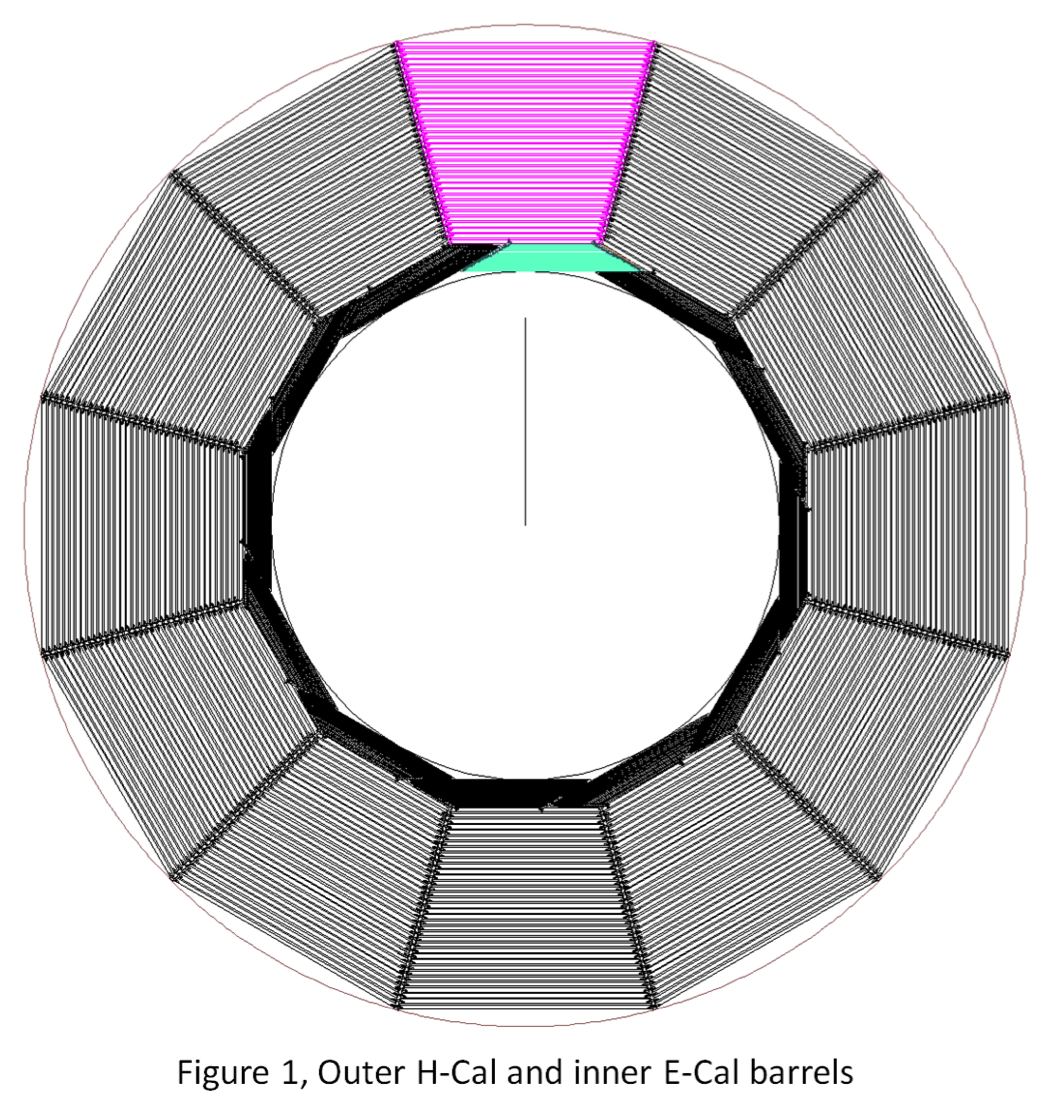
\includegraphics[width=\linewidth]{Calorimeter/SiliconTungstenSiD/cross_section}
		\caption{Outer HCAl and inner ECal barrel}
		\label{fig:Calorimeter:SiDECAL:crosssection}
	\end{minipage}\hfill
	\begin{minipage}[b]{.49\textwidth}
		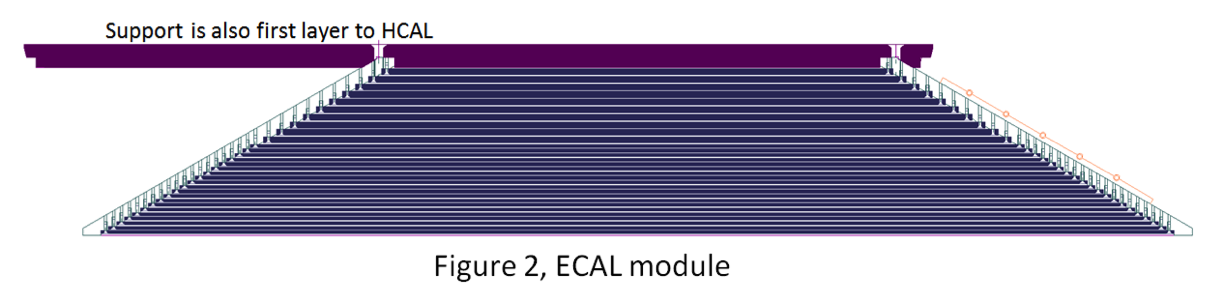
\includegraphics[width=\linewidth]{Calorimeter/SiliconTungstenSiD/ecalModule}
		\caption{ECal module}
		\label{fig:Calorimeter:SiDECAL:ecalModule}
	\end{minipage}
\end{figure}
\begin{figure}
	\begin{minipage}[b]{.29\textwidth}
		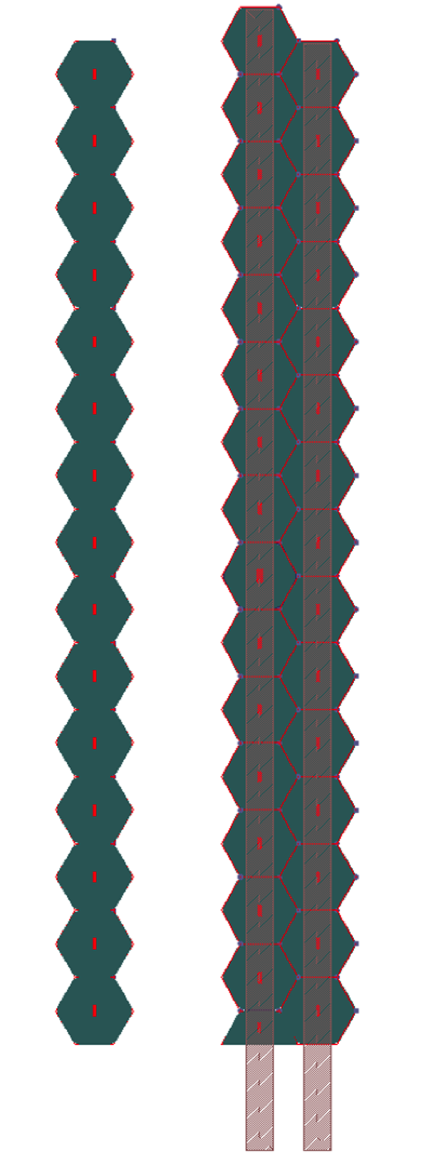
\includegraphics[width=\linewidth]{Calorimeter/SiliconTungstenSiD/hexagon}
		\caption{Hexagonal silicon detectors with flexible circuit interconnects}
		\label{fig:Calorimeter:SiDECAL:hexagon}
	\end{minipage}\hfill
	\begin{minipage}[b]{.65\textwidth}
		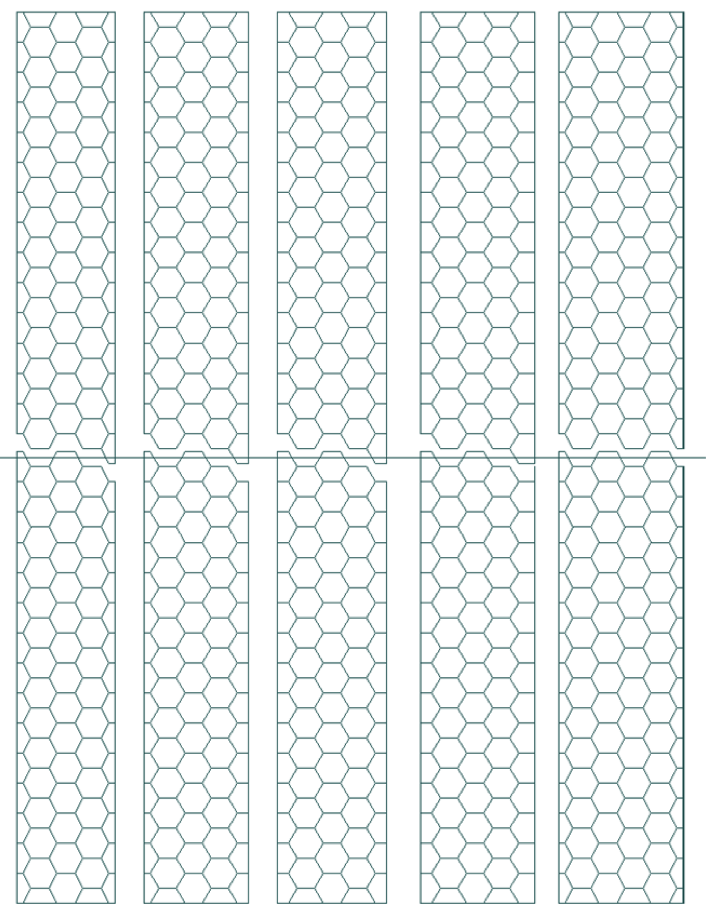
\includegraphics[width=\linewidth]{Calorimeter/SiliconTungstenSiD/siliconLayout}
		\caption{Silicon layout for five outer layers}
		\label{fig:Calorimeter:SiDECAL:siliconLayout}
	\end{minipage}
\end{figure}
\begin{figure}
	\begin{minipage}[b]{.49\textwidth}
		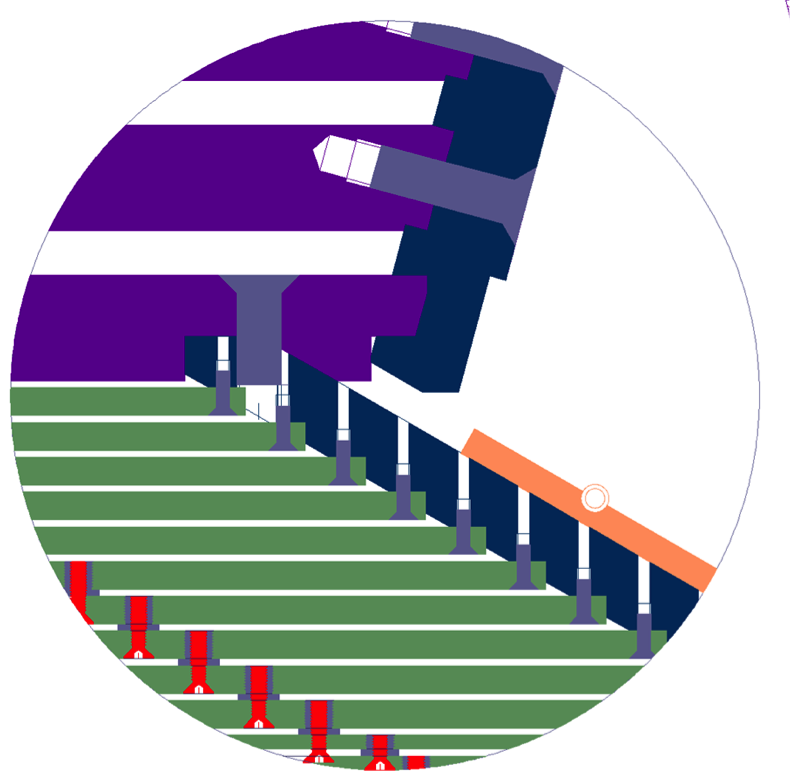
\includegraphics[width=\linewidth]{Calorimeter/SiliconTungstenSiD/edgeFasteners}
		\caption{Edge and field fasteners}
		\label{fig:Calorimeter:SiDECAL:edgeFasteners}
	\end{minipage}\hfill
	\begin{minipage}[b]{.49\textwidth}
		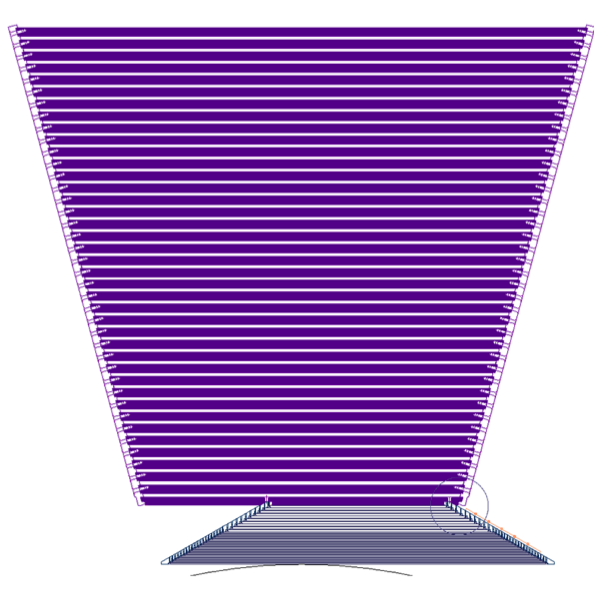
\includegraphics[width=\linewidth]{Calorimeter/SiliconTungstenSiD/ecalMounting}
		\caption{ECal to HCal mounting}
		\label{fig:Calorimeter:SiDECAL:ecalMounting}
	\end{minipage}
\end{figure}
\begin{figure}
	\begin{minipage}[b]{.49\textwidth}
		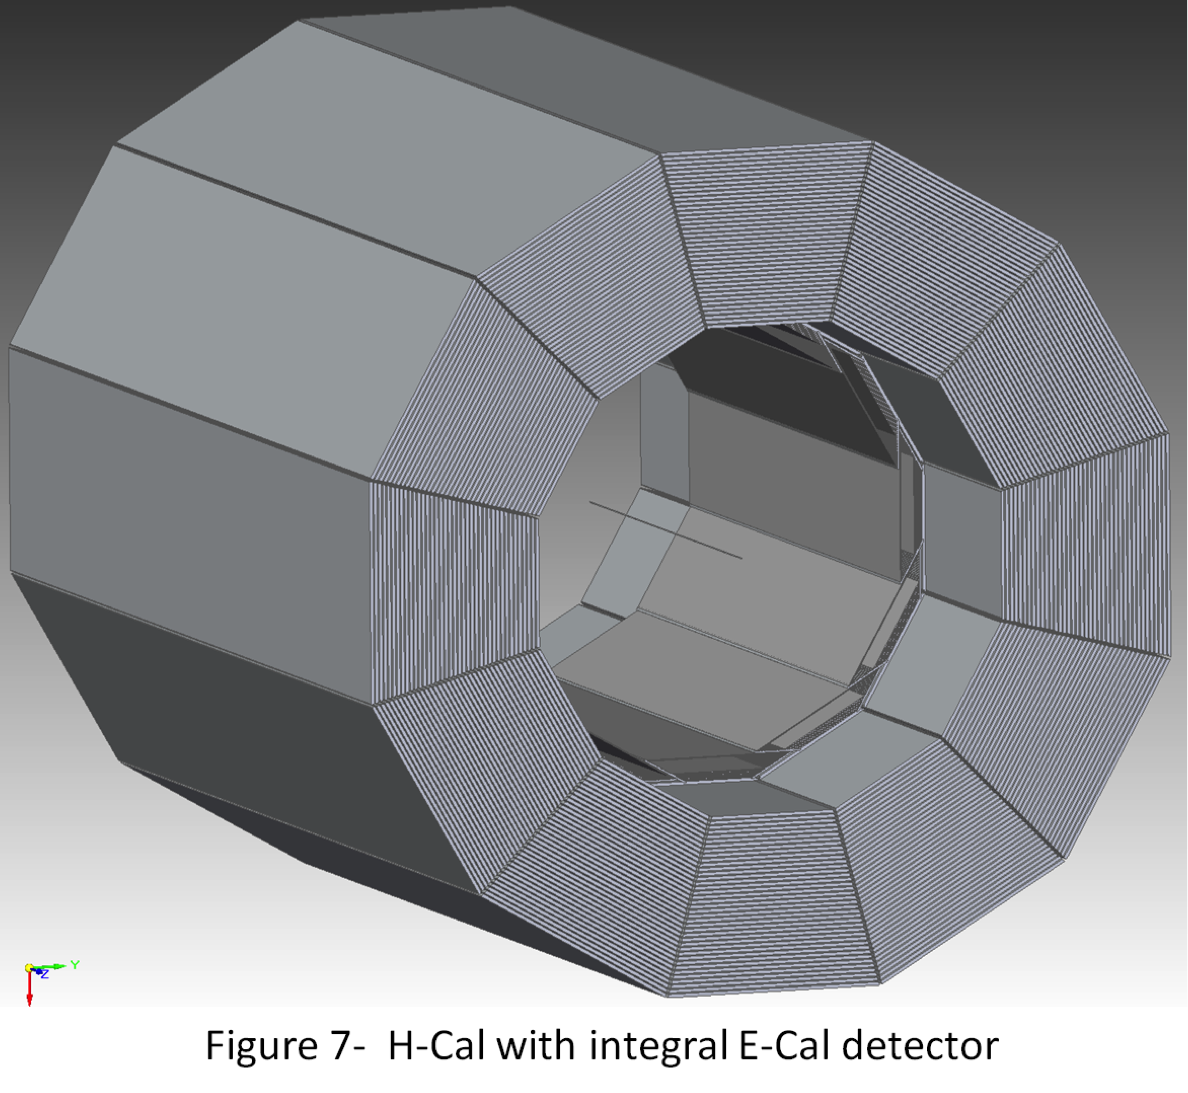
\includegraphics[width=\linewidth]{Calorimeter/SiliconTungstenSiD/HCalECal}
		\caption{HCal with integral ECal detector}
		\label{fig:Calorimeter:SiDECAL:HCalECal}
	\end{minipage}\hfill
	\begin{minipage}[b]{.49\textwidth}
		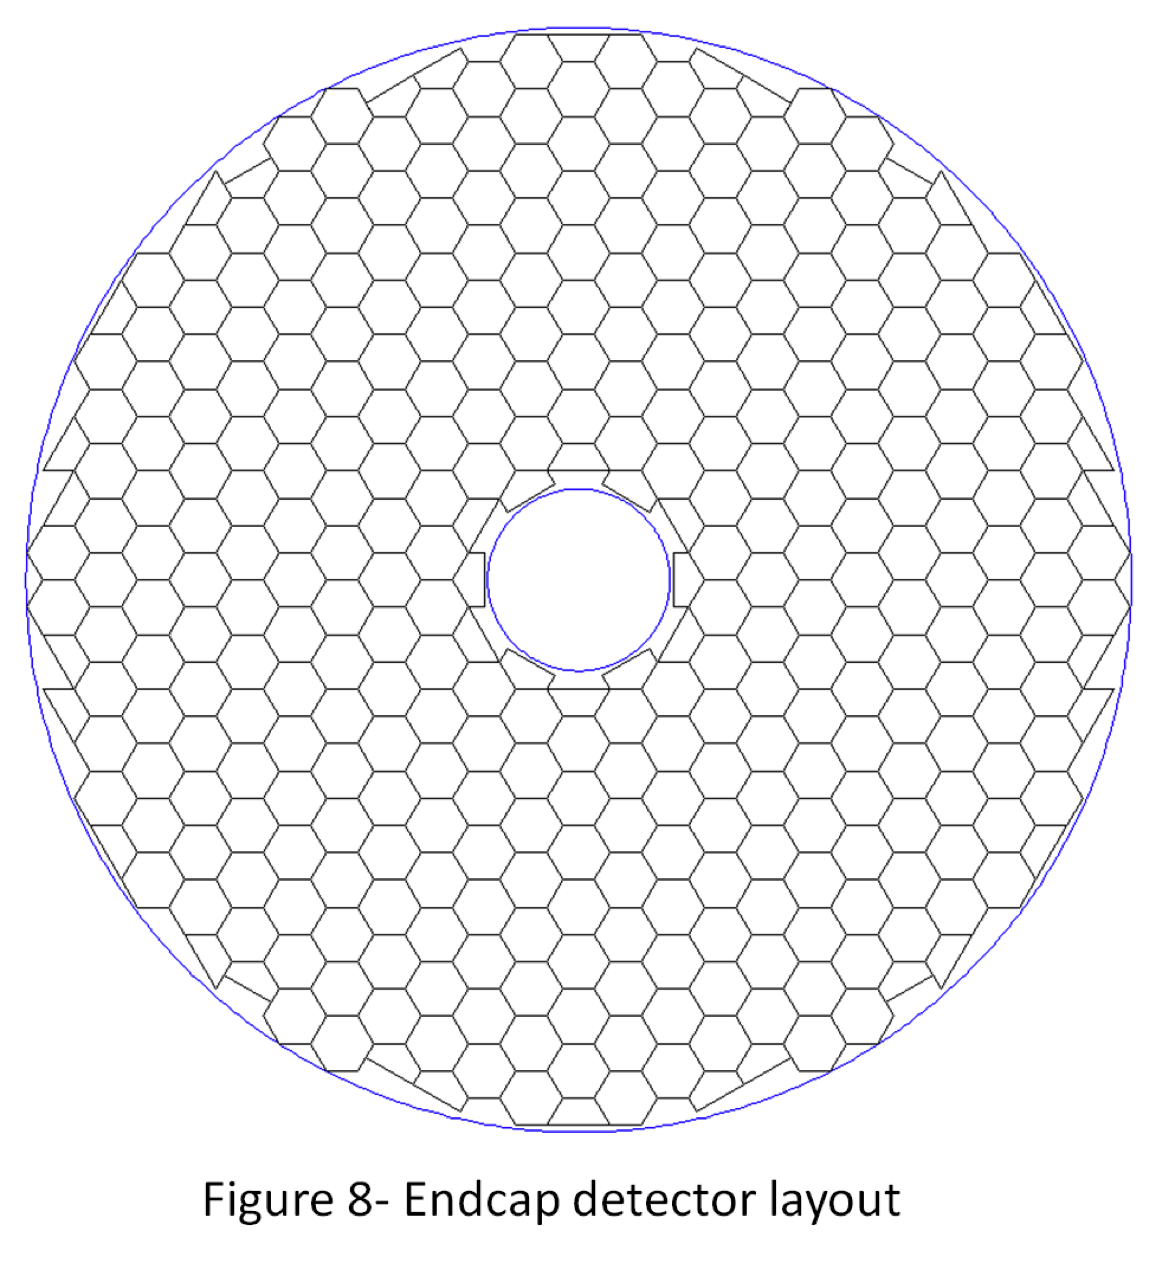
\includegraphics[width=\linewidth]{Calorimeter/SiliconTungstenSiD/endcapLayout}
		\caption{Endcap detector layout}
		\label{fig:Calorimeter:SiDECAL:endcapLayout}
	\end{minipage}
\end{figure}

This note describes the theory of the mechanical aspects of the E-Cal system for
SiD. The E-Cal barrel consists of stacks of tungsten heavy metal plates which
are arranged in modules surrounding the beamline. Full cylindrical coverage of
the baseline design is attained with twelve modules (see Figure~\ref{fig:Calorimeter:SiDECAL:crosssection}) occupying a
radial envelope from \unit[1265]{mm} to \unit[1409]{mm}. The total barrel length is \unit[3.53]{m}. Each
module uses 20 inner plates which are \unit[2.5]{mm} thick followed by ten \unit[5]{mm} thick
plates. Gaps between adjacent plates are \unit[1.25]{mm} and house the silicon detectors
with their associated cables (see Figure~\ref{fig:Calorimeter:SiDECAL:ecalModule}). These hexagonal silicon detectors
are electrically connected to each other with thin, flexible circuits which are
read out on both ends of a module (see Figure~\ref{fig:Calorimeter:SiDECAL:hexagon}). Panels of detectors increase
in width as they get closer to the beamline. To minimize silicon waste and to
maximize coverage, fractions of hexagons complete the panel edges (see Figure~\ref{fig:Calorimeter:SiDECAL:siliconLayout}). By cutting the silicon in strategic locations, only a few different silicon
shapes may be needed to achieve the 31 different panel widths. The tungsten
plates are connected together on their longitudinal edges as well as in the
field of detectors. Space for fasteners in the field is achieved by chamfering
the corners of the hexagonal detectors. The field fasteners hold the plates
together, provide a uniform \unit[1.25]{mm} standoff height, and assist with inter-plate
shear. The fasteners near the edges of the plates close the module profile and
lend torsional rigidity to the structure. An FEA simulation of the proposed
configuration should be done to properly size the fasteners (see Figure~\ref{fig:Calorimeter:SiDECAL:edgeFasteners}).The
modules, which weigh about 5 tons each, are mounted to stainless plates which
are used as the first layer of the next detector system (H-Cal). This first
H-Cal plate is unique in that its two longitudinal edges form a guide system to
locate the E-Cal to the H-Cal system. The H-Cal modules are first bolted
together to form the H-Cal barrel. Interleaving structural side battens maintain
spacing for the H-Cal plates and extend inward to the E-Cal support plates. The
inner ends of these battens act in concert as the female portion of the E-Cal
guide system. The E-Cal modules are slid into place in the inner H-Cal bore.
Extension plates complete the inner H-Cal first layer, since the E-Cal barrel is
shorter. H-Cal detector panels are installed after this structure is complete
(see Figure~\ref{fig:Calorimeter:SiDECAL:HCalECal}). Only simple detector layouts have been done for the E-Cal
endcaps so far. These layouts show that using full and partial hexagons could
yield fairly good coverage with only a few shapes. (see Figure~\ref{fig:Calorimeter:SiDECAL:endcapLayout}).

% \subsection{Participating Institutes}
% SLAC National Accelerator laboratory
% University of California, Davis
% University of California, Santa Cruz
% University of Oregon
% University of New Mexico

\subsection{Introduction}
KPiX is a 1,024 channel ``System on a Chip'' intended for bump bonding to large area Si sensors, enabling low multiple scattering Si strip tracking and high density Particle Flow calorimetry for SiD at the International Linear Collider (ILC).

Each channel consists of a dynamically switchable gain charge amplifier; shaping; threshold discrimination; and 4 sample and hold capacitors and 4 timing registers. The chip permits 4 separate measurements of amplitude and time of threshold crossing during each train, and amplitude digitization and readout during the intertrain period. The dynamic range is from sub minimum ionizing particle (mip) (\unit[320]{\micron} silicon) to more than 2,000 mip. KPiX also has a calibration system for each channel, servos for leakage compensation, ``DC'' reset for asynchronous operation for testing with cosmic rays, and polarity inversion for use with GEMs and similar detectors. The noise floor is about \unit[0.15]{fC} ($\approx 1,000$ electrons), and the maximum signal is \unit[10]{pC} (utilizing the dynamic range switching). The full dynamic range corresponds to 17 bits.

\subsection{Recent Milestones}
ILC related R\&D in the US is largely unfunded and small efforts are being kept alive on the margins. The KPiX R\&D is such an example of necessary work for SiD that is marginally alive.
At this time, KPiX is seen as the baseline readout system for the tracker and electromagnetic calorimeter .  A stack of 13 EMCal sensors with bump bonded KPiX was assembled for a beam test at SLAC in the summer of 2013. That test discovered that two kinds of crosstalk are significant:
\begin{itemize}
	\item In-time crosstalk occurs due to parasitic coupling of traces on metal 2 of the sensor to other pixels. The level of crosstalk increases with the size of the signal, and decreases with increased speed of the front end charge amplifier (meaning increased current and power dissipation).  A new sensor design is being developed that uses metal 1 to shield the traces of metal 2, and these ideas will be tested in the next sensor prototype.
	\item Out-of-time cross talk occurs when many pixels are hit and reset simultaneously. The resets collectively cause other pixels to trigger, and a cascade builds up. This uses up all the KPiX buffers. The root cause of the problem appears to be some internal logic within KPiX that is not current limited, and will require design modification.
\end{itemize}
A more general issue is that both the EMCal and tracker sensors from Hamamatsu were ordered with Al pads, as it was believed that plating (by the zincate process) a stack of metals culminating with Au would be straightforward. This turns out to be wrong. After many attempts at University of California Davis (UCD) and local industry, IZM  has Ar ion etched the pad surfaces and sputtered a base layer, permitting the buildup of a stack that ended with Au, and permitting the attachment with solder bumps that had been placed during KPiX manufacture by TSMC. Testing of these sensors revealed $\approx 10\%$ pixel to pixel shorts and some opens of signal traces, that are suspected to be damage caused by the Ar ion etch. A new round of sensors has been ordered with the Metal 1 layer used to shield the Metal 2 traces from the diodes that they cross on the way to the KPiX bump pads, and with the Au pads being built by Hamamatsu.

An additional issue is that the Tracker sensor was planned to be wire bonded to its (very thin) cable. The sensor oxide layer is not strong enough to allow wire bonding without damage, and so must be solder bumped. The pad pitch is small, and solder bumping the cable will be challenging. The trouble with the wire bonding to the sensor was unexpected. Recent attempts with both bump bonding a cable and utilizing electrically conductive epoxy have failed. The best explanation is that the \unit[150]{\textdegree C} thermal cycles associated with these attachments increased the stress on the KPiX bonds and caused the sensor pads to separate from the sensor. It is belived that something went wrong with the Hamamatsu process on both types of sensors, and is related to the wire bonding problem.

Another concern is that the current design of KPiX has deadtime after a pixel has accepted a trigger. Only the triggered pixel is affected; all the other pixels are available for signals. This deadtime is different from the usual notion of data acquisition deadtime where the entire detector is unavailable, but the correction to the luminosity integral is easy. Finally, the buffer requirement (4 in the current version of KPiX) is being re-evaluated in SiD simulations. A possible new architecture for KPiX is in early stages of evaluation. Another approach is the development of Monolithic Active Pixel (MAP) sensors for both SiD sensors using thinned HVCMOS. The sensors would be approximately the same size as the current sensors. The tracker would have $40 \times \unit[500]{\micron}$ pixels, and would only need one buffer. A prototype to evaluate the pixel performance is being designed now. The EMCal sensor will have $1 \times \unit[1]{mm}$ pixels which should limit the required dynamic range and eliminate range switching, but would still need 16 buffers.

A small mechanical engineering effort has started to study the structure of the EMCal. The Sid EMCal has emphasized thin gaps between the tungsten layers to minimize the Moliere radius, and this implies that the structure is connected by columns at the vertices of the sensors. This work has been carried out to the level of a pre-conceptual design.

\subsection{Engineering Challenges}
\subsection{Future Plans}
Assuming positive developments with Japan are announced soon, we expect the financial support to improve. It should be noted that an important effect of the withdrawal of support is that most of the US collaborators have been forced to move to other work.
\begin{itemize}
	\item EMCal Sensors: A second round of prototypes will be designed and ordered with rectangular layout; shielded traces, and Au pads.
	\item Tracker Sensors: The current prototypes will be evaluated, and if appropriate tested in a beam.
	\item KPiX: A new architecture with little (or no) deadtime will be evaluated. A decision will be made to develop this new architecture or incrementally improve the existing design.
	\item The EMCal mechanical structure will be pushed towards a conceptual design.
\end{itemize}

%from arXiv:1212.5127v2
\section{DECAL}

The studies of a digital ECAL (DECAL) continue in the UK, in spite of very significant
funding difficulties. In December 2008, the STFC Executive recommended sufficient funding
to allow the SPiDER Collaboration to construct a full physics prototype DECAL, as outlined
in~\cite{Adloff:2010aa}. By December 2009, the funding for SPiDER had still not been issued and STFC
informed the Collaboration that they would not do so.

The UK groups in SPiDER have demonstrated that the INMAPS technology developed
specifically for the DECAL application is viable in terms of basic pixel efficiency. INMAPS is
implemented as a \unit[0.18]{\micron} CMOS process in which a deep P-well implant stops signal charge
from being absorbed in N-well circuits, and therefore allows the use of both NMOS and
PMOS within the pixel, as well as (optionally) high resistivity silicon in the thin epitaxial
layer to reduce the charge collection time.

\subsection{Test Beams in 2010}
Following a successful test beam run at CERN in September 2009 using 120 GeV pions, two
further data taking runs have been carried out. The first of these was at DESY in March
2010, for which the primary goal was to quantify the peak electromagnetic shower density
observed downstream of specific absorber materials. A secondary goal was to make further
pixel efficiency measurements. Data were recorded with the 1-5 GeV electron beam, using a
configuration in which four TPAC 1.2 sensors were aligned precisely along the beam direction
using the same custom-built mechanical frame as at CERN. Absorber material (W, Fe, Cu)
was placed downstream of these, followed immediately by a further pair of TPAC sensors, to
study the shower density.

To complement the DESY run, similar, additional data was recorded at CERN in September 2010, using the EUDET telescope alone as it has finer pitch than the TPAC sensor, with positrons between 10 and 100 GeV. The same slabs as those at DESY were used together with
new slabs due to the higher energies available at CERN. Initial results of shower multiplicities
are presented in~\cite{Price:2012vta}.

\subsection{Pixel efficiency results}
The studies of pixel efficiency from CERN 2009 testbeam and DESY were performed using a
set of six TPAC 1.2 sensors aligned along the beam direction, in which the outer four sensors
served as a beam telescope, while the two innermost sensors were considered as the devices
under test. The trajectory of the beam particle was projected onto the plane of both of these
sensors, and each pixel of the test sensors was examined for the presence of hits as a function
of the distance from the projected track. The MIP hit efficiency was determined by fitting
the distribution of hit probability to a flat top function, convoluted with a Gaussian of the
appropriate resolution to allow for finite tracking performance. This efficiency, folded for all
pixels together, is illustrated in Figure~\ref{fig:Calorimeter:DECAL:MIPS}

\begin{figure}
    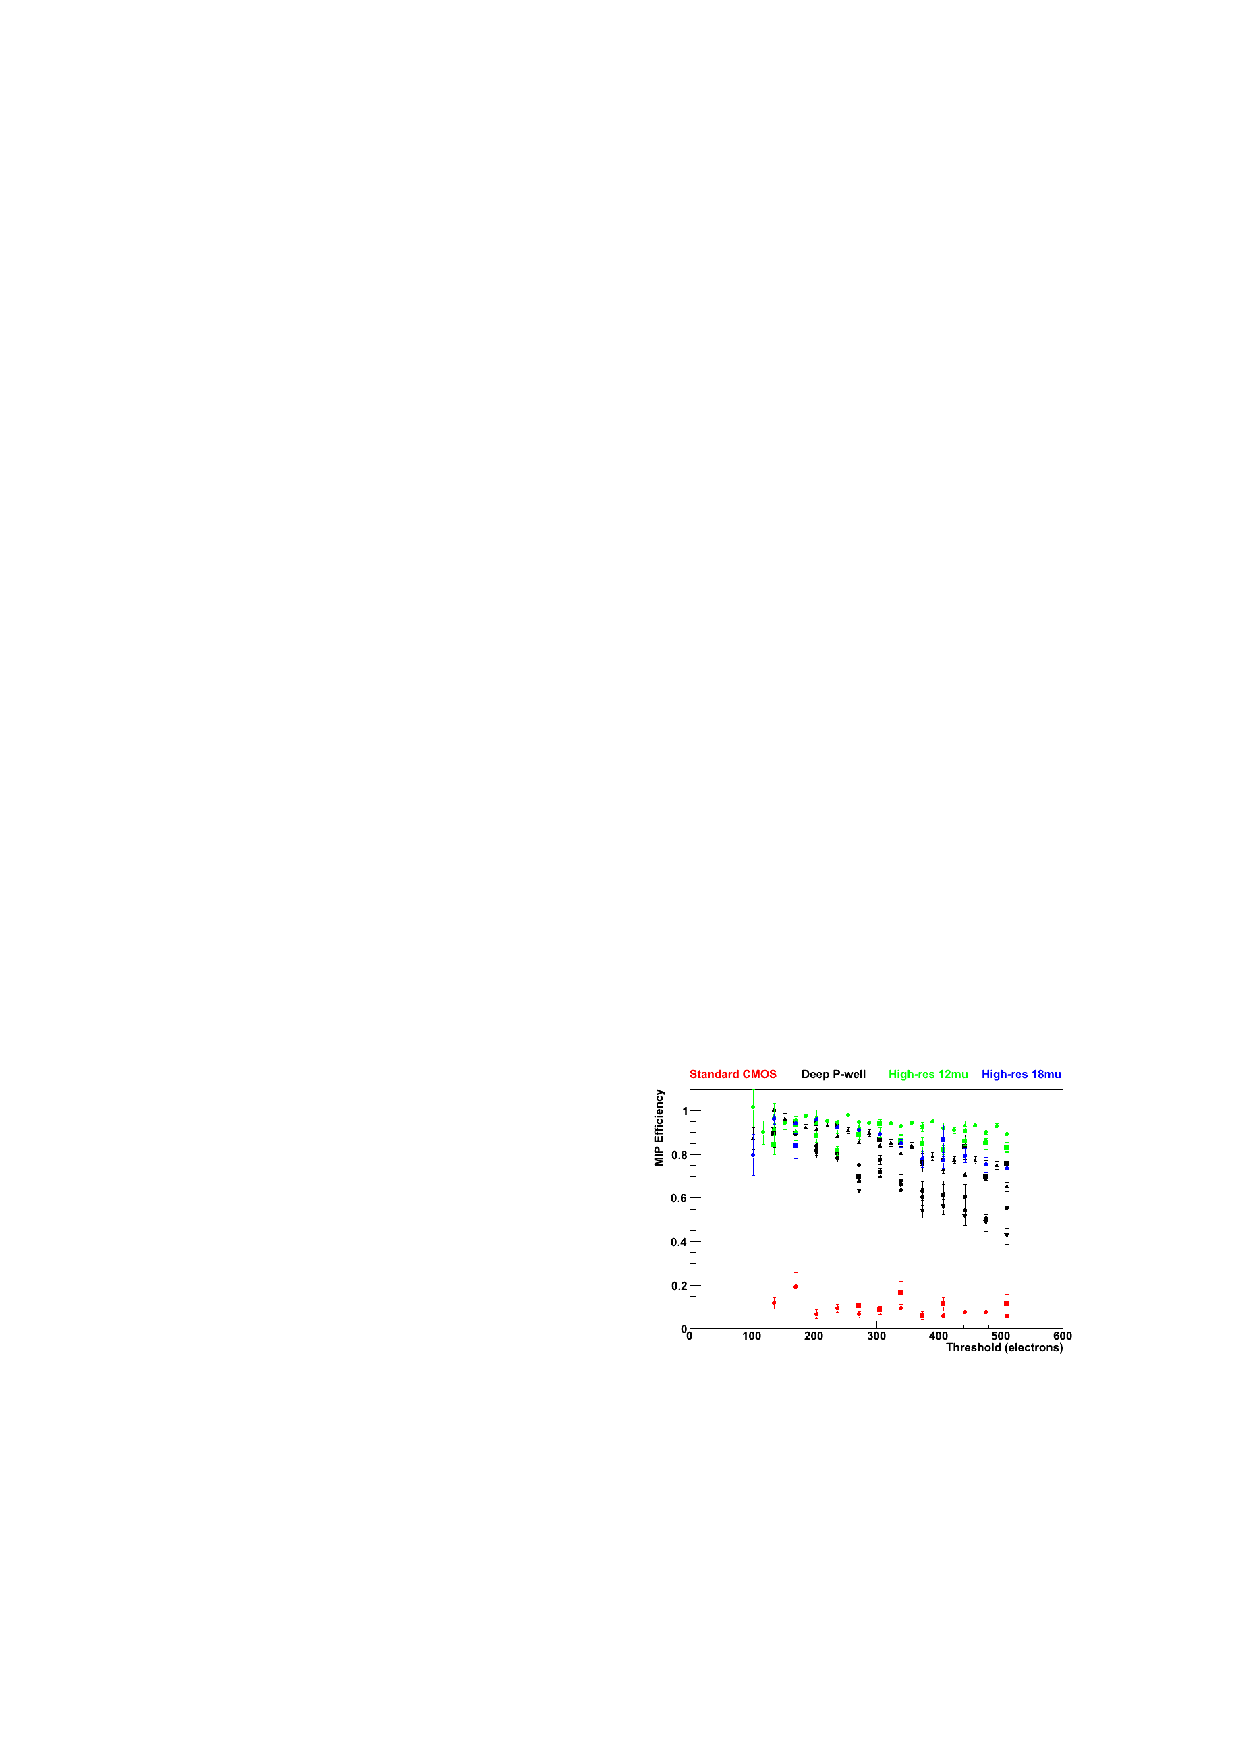
\includegraphics[width=.49\textwidth]{Calorimeter/DECAL/MIPEfficiency}
    \includegraphics[width=.49\textwidth]{Calorimeter/DECAL/MIPResponse}
    \caption{(left) Distribution of the probability of a pixel registering a hit in response to a MIP, as a function of distance to the projected track, and (right) MIP efficiency as a function of the sensor digital threshold, for all four sensor variants studied.}
    \label{fig:Calorimeter:DECAL:MIPS}
\end{figure}

The MIP efficiency was determined per pixel for both the DESY and CERN data, and for each of the four pixel variants tested. The variants (and corresponding marker color in Figure~\ref{fig:Calorimeter:DECAL:MIPS}) are:

\begin{enumerate}
\item (red) in \unit[12]{\micron} standard (non-INMAPS) CMOS;
\item (black) \unit[12]{\micron} deep P-well CMOS;
\item (green) deep P-well within a \unit[12]{\micron} high resistivity epitaxial layer;
\item (blue) deep P-well within an \unit[18]{\micron} high resistivity epitaxial layer.
\end{enumerate}

The results~\cite{Dauncey:2010zz} are summarized in Figure~\ref{fig:Calorimeter:DECAL:MIPS}, for a range of the sensor digital thresholds representative of the signal levels expected in DECAL pixels due to charge spreading. (A typical MIP signal in a \unit[12]{\micron} epitaxial layer of silicon is 1200 electrons and a single pixel absorbs at most 50\% of this due to charge spreading.)

From the results shown in the figure, it is observed that the standard, non-INMAPS sensors have markedly low efficiencies, which is attributed to signal charge being absorbed by in-pixel PMOS transistors. In contrast, the use of the deep P-well reduces the absorption of signal charge by N-wells in the circuitry, improving very substantially the pixel efficiency by a factor of $\approx 5$. The addition of the high resistivity epitaxial layer further improves the pixel efficiency to $\approx 100\%$.

\subsection{Future plans}
It is no longer an option to plan for a physics prototype DECAL and the short-term future of the DECAL project is extremely uncertain at present. A program of radiation hardness has been conducted on 2011 and the results are summarized in~\cite{Price:2012vta,Price:2013js}. This is in part to understand how the TPAC sensor would satisfy the requirements of ALICE ITS and SuperB . The studies which have been carried out so far are in the process of being finalized, and a series of papers, e.g.~\cite{Ballin:2011jq}, are in preparation to document what has been achieved. The technology development has been taken over by the Arachnid collaboration who are testing the CHERWELL chip (designed and manufactured by the SPiDeR collaboration but never used due to money constraints) to evaluate the performance for ALICE and SuperB.


\section{Resistive Plate Chambers}

\subsection{Description of the DHCAL}
The Digital Hadron Calorimeter or DHCAL uses Resistive Plate Chambers (RPCs) as active elements. The chambers are read out with $\unit[1 \times 1]{cm^2}$ pads and 1-bit (digital) resolution. A small-scale prototype was assembled and tested in the Fermilab test beam in 2007 to validate the concept.
Based on the success of the small-scale test [1-6], a large prototype with up to 54 layers and close to 500,000 readout channels was built in 2008 -- 2011. Each layer measured approximately $\unit[96 \times 96]{cm^2}$ and was equipped with three chambers, stacked vertically on top of each other.
For tests with particle beams the DHCAL layers were inserted into a main stack of 38 or 39 layers, followed by a tail catcher with up to 15 layers. For the tests performed at Fermilab the main stack contained steel absorber plates. At CERN the absorber plates contained a Tungsten based alloy. In both cases the tail catcher featured steel absorber plates.
In the various test beam campaigns combined, spanning the years 2010 -- 2012, the DHCAL recorded of the order of 14 Million muon events and 36 Million secondary beam events, where the latter contained a mixture of electrons, muons, pions, and protons.
\subsection{Current R\&D activities}
The analysis and publication of the test beam results are currently the highest priority of the DHCAL group. Major challenges, such as the calibration (or equalization) of the response of the RPCs and the detailed simulation of the response of RPCs, are very close to having been overcome [7-11].
In parallel, to the analysis of test beam data, the group is pursuing the following R\&D activities:
\subsubsection{Development of 1--glass RPCs}
The DHCAL prototype featured a standard chamber design based on RPCs with two resistive plates. The Argonne group, however, proposes to eliminate one of the glass plates in future applications. The advantages are: close to unit pad multiplicity with significant simplification of the calibration and monitoring procedure, reduced thickness of the active element, higher rate capability, and insensitivity of the response to the surface resistivity of the resistive layer (used to apply the High Voltage). To date several 1-glass RPCs have been assembled. The chambers tested very well with cosmic rays. Tests in particle beams are planned for future test beam campaigns.
\subsubsection{Development of high-rate RPCs}
Due to the high bulk resistivity of glass (and Bakelite), RPCs are notoriously rate limited [12]. The DHCAL group is addressing this shortcoming with the development of semi-conductive glass (in cooperation with COE college) and of low-resistivity Bakelite (in co-operation with USTC). First chambers with samples of low-resistivity glass plates have been assembled and have tested in the Fermilab test beam.
\subsubsection{Development of a High-Voltage distribution system}
With up to 50 layers in a single calorimeter module, a cost-effective way to distribute the High-voltage to individual layers is required. A system capable to regulate the voltage within a few 100 V, to monitor both the current and the voltage, and to switch off individual channels, is being developed. A first prototype controlling a single channel has been assembled and tested successfully with an RPC. The development is currently on hold due to lack of funding.
\subsubsection{Development of a gas recycling system}
The operation of RPCs requires a gas mixture, which is both costly and environmentally harmful. To limit the effect of releasing gas into the environment, the DHCAL group is developing a gas recycling system. The system is based on a new approach, appropriately labeled ``Zero Pressure Containment''. A prototype of the gas collection subsystem is currently being assembled; however, progress is again slow due to lack of funding.
\subsubsection{Development of the next generation front-end readout system}
The next generation front-end readout system will contain several upgrades compared to the current system: higher channel count, token ring passing, low power operation, power pulsing, and improved internal charge injection systems. To proceed, the project is awaiting funding from both US and Chinese agencies.

\subsection{Engineering challenges}
Several engineering challenges remain to be addressed before an RPC-based DHCAL can be proposed as an option for a colliding beam detector. Following is an (incomplete) list of the major issues:
\begin{itemize}
\item Industrialization of the construction of RPCs.
\item Design of the readout boards, covering the entire area of the layer (with varying width). The design is expected to feature only a minimum number of different boards.
\item Design of the gas distribution system, which ensures equal pressure in all layers of a given module, independent of its orientation.
\item Development of a cooling strategy for the front-end boards, which will include power pulsing, as well as active cooling.
\item Development of a module assembly procedure.
\end{itemize}

\subsection{Plans for the coming years}
The activities of the coming years depend strongly on the progress with the Japanese intentions to host the ILC. Assuming the ILC project goes ahead, the DHCAL group will
a)  Complete the analysis and publication of the test beam data,
b)  Complete the R\&D projects listed above, and
c)  Start the development of the design of calorimeter modules.
In case, the ILC is not going forward, the group plans on completing the data analysis and to continue the tests of high-rate RPCs. Other R\&D projects, such as the development of distribution systems, will be put on hold.

\subsection{Applications beyond the ILC}
The DHCAL technology was specifically developed for the hadron calorimeter of the ILC, with its low particle rate and radiation dose. To export the technology to other environments, the rate capability of the chambers and the radiation hardness of the readout need to be improved. The former is being addressed with low-resistivity plates (glass and Bakelite), while the latter will require a new front-end readout system based on an ASIC using a smaller feature size. Possible applications are the tail catcher of the forward calorimeters of CMS and the outer wheels of the ATLAS muon system. Both options are being pursued actively.

References
\begin{enumerate}
\item \fullcite{Drake200788}
\item \fullcite{1748-0221-3-05-P05001}
\item \fullcite{1748-0221-4-04-P04006}
\item \fullcite{1748-0221-4-06-P06003}
\item \fullcite{1748-0221-4-10-P10008}
\item \fullcite{1748-0221-5-02-P02007}
\item \fullcite{Repond:2011:CAN30}
\item \fullcite{Repond:2013:CAN30A}
\item \fullcite{Xia:2011:CAN31}
\item \fullcite{Xia:2011:CAN32}
\item \fullcite{Repond:2012:CAN39}
\item \fullcite{Bilki:2013:CAN42}
\item \fullcite{Xia:2014:RPC2014}
\end{enumerate}

\section{GEM}
\subsection{Introduction}
The group pursues the development of Gas Electron Multiplier technology for instrumenting a digital hadronic calorimeter (DHCAL) at the ILC. The 
\subsection{Recent Milestones}
\subsection{Engineering Challenges}
\subsection{Future Plans}
\begin{itemize}
\item To be determined
\end{itemize}
\subsection{Applications Outside of Linear Colliders}

\section{THGEM-based sampling elements for DHCAL}
\subsection{Introduction}
Digital Hadronic Calorimetry (DHCAL) for future experiments (e.g. ILC-SiD) requires robust thin sampling elements with high detection efficiency at low pad multiplicity. The large detection area foreseen requires cost-effective solutions.
In the past two years, a Weizmann-Aveiro-Coimbra team has shown that sampling elements based on Thick Gaseous Electron Multipliers (THGEM)~\cite{Chechik2004303} could meet DHCAL requirements. The THGEM concept has evolved from a cascade of double-sided electrodes coupled to a pad-anode through an induction gap~\cite{1748-0221-7-05-C05011}, to thinner single-sided WELL detectors - coupled to the pads with and without resistive films~\cite{1748-0221-9-04-P04011,1748-0221-8-07-P07017}.
The most recent and presently leading candidate is the Resistive Plate WELL (RPWELL). It was tested extensively in the laboratory~\cite{1748-0221-8-11-P11004,1748-0221-8-12-C12012} and at muon and high-rate pion beams at CERN-SPS. This very thin single-stage detector yielded a discharge-free operation in different gas mixtures, including Ne- and Ar-based ones, providing high detection efficiency at low pad multiplicity.

\subsubsection{The Resistive Plate WELL}
The Resistive Plate WELL (RPWELL) is a single-sided THGEM (with copper clad on one side only), coupled to the readout pads through a material sheet with high bulk resistivity (see Figure~\ref{fig:Calorimeter:THGEM:rpwell}). Materials with bulk resistivity in the $\unit[10^9]{\Omega cm}$ scale prevent significant gain-, and hence efficiency drops, at high particle flux~\cite{1748-0221-8-11-P11004}.
\begin{figure}
	\centering
	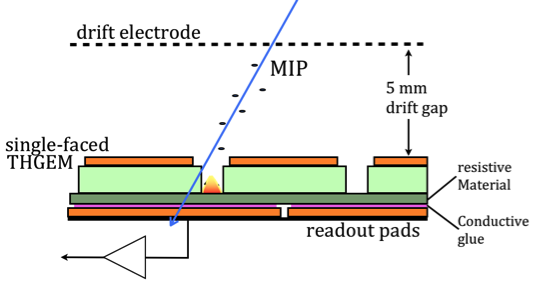
\includegraphics[width=.5\textwidth]{Calorimeter/THGEM/rpwell.png}
	\caption{The RPWELL configuration with a resistive anode and a readout electrode. The WELL, a single-faced THGEM, is coupled to a readout anode (e.g. with strips or pads) via a resistive plate.}
	\label{fig:Calorimeter:THGEM:rpwell}
\end{figure}
\subsection{Recent Milestones}
Small ($\unit[10\times 10]{cm^2}$) and medium size ($\unit[30\times 30]{cm^2}$) RPWELL detector prototypes were built and tested in the laboratory and at the CERN-SPS. The \unit[0.8]{mm} thick WELL electrodes were coupled to $\unit[1\times 1]{cm^2}$ copper pads through \unit[0.4]{mm} thick Semitron ESD225 resistive polymer ($\approx \unit[10^9]{\Omega cm}$ bulk resistivity). With a \unit[5]{mm} drift gap the sampling element had a total thickness of \unit[6.2]{mm} (excluding readout electronics – here SRS-APV~\cite{1748-0221-8-03-C03015,French2001359}).
The detection efficiency as a function of pad multiplicity (with low rate muons) is shown for the two prototypes in Figure~\ref{fig:Calorimeter:THGEM:efficiencyVSMultiplicity}. Both detectors reached high detection efficiency at low pad multiplicity when operated in our traditional Ne/5\%\ce{CH4} (Figure~\ref{fig:Calorimeter:THGEM:efficiencyVSMultiplicity} left; operation voltage, V, in the range $800-\unit[930]{V}$) and in the cost-effective Ar/5\%\ce{CH4} (Figure~\ref{fig:Calorimeter:THGEM:efficiencyVSMultiplicity} right; V in the range $1500-\unit[1720]{V}$) gas mixtures.
\begin{figure}
	\centering
	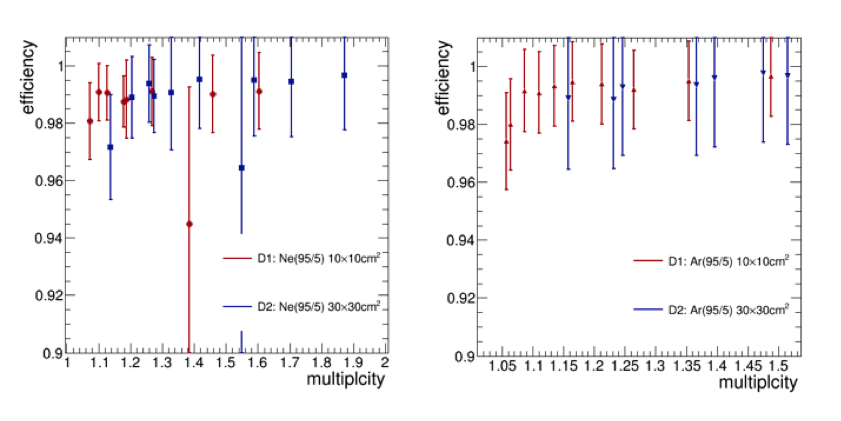
\includegraphics[width=.9\textwidth]{Calorimeter/THGEM/efficiencyVSMultiplicity.png}
	\caption{Efficiency as a function of the average pad multiplicity measured with the $\unit[10\times 10]{cm^2}$ and $\unit[30\times 30]{cm^2}$ detectors in muon beam. Left: Ne/5\%\ce{CH4} gas mixture. Right: Ar/5\%\ce{CH4} gas mixture}
	\label{fig:Calorimeter:THGEM:efficiencyVSMultiplicity}
\end{figure}
\begin{figure}
	\centering
	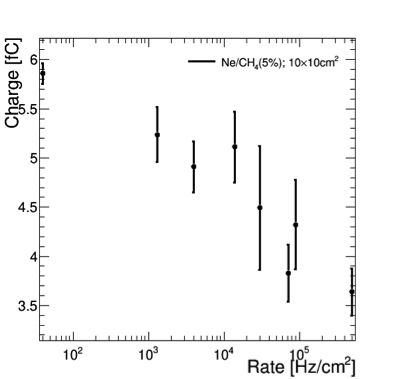
\includegraphics[width=.5\textwidth]{Calorimeter/THGEM/charge_vs_rate.png}
	\caption{The charge (estimated from the spectra most probable value) as a function of the incoming particle flux.  All the measurements were conducted at Ne/5\%\ce{CH4} gas mixture at the same operation voltage of \unit[880]{V}. A pion beam was used to generate the high incoming fluxes.}
	\label{fig:Calorimeter:THGEM:chargeVsRate}
\end{figure}
Figure~\ref{fig:Calorimeter:THGEM:chargeVsRate} shows the measured gain as a function of the particle flux; the same operation voltage of \unit[880]{V} was maintained throughout the measurements (with low rate muons as well as high rate pions). A moderate gain-drop of $\approx 30\%$ was measured while the flux was increased by 3 orders of magnitude (from 50 to $\unit[10^5]{Hz/cm^2}$). It resulted in negligible efficiency drop, since the pulse-over-threshold was sufficiently high.
Most importantly, during the two weeks of in-beam operation (which included also long time operation under high rate, $\unit[10^5]{Hz/cm^2}$, pion beam), with both Ne-based and Ar-based gas mixtures, the small prototype was completely discharge-free. The resulting discharge probability is therefore below $10^{-8}$. Occasional discharges occurring in the medium-size prototypes were traced to be associated with defects in some support pins within the active area; these can be avoided in the next prototypes.
The RPWELL laboratory and test-beam results are the subject of two articles in preparation.


\subsection{Engineering Challenges}
The novel design of a large RPWELL detector prototype (without the present support pins) is completed. Assembly and tests are foreseen in the coming year. Upon success, we are confident that future chambers could be fully industrially produced.
We are currently investigating, with industry, alternative materials and production technologies of THGEM electrodes; similarly, we are considering different resistive-plate materials, with of appropriate bulk resistivity.

\subsection{Future Plans}
As mentioned earlier, in the forthcoming year we intend to build a new medium-size detector prototype, to be followed by a prior to our square-meter one. Both prototypes will be tested in the laboratory and in muon and pion beams (CERN).
We foresee investigating the properties of several RPWELL layers in a fully-equipped DHCAL prototype; in particular their performance in measuring Hadronic showers.

\subsection{Applications Outside of Linear Colliders}
So far, our studies of THGEM-based detectors, particularly the RPWELL, have yielded a cost-effective, single-stage completely stable device, with wide dynamic range. The RPWELL concept is suitable for a variety of applications that do not require very high spatial and energy resolutions. Current examples are CsI-coated multipliers for UV-photon imaging in RICH detectors; cryogenic gaseous photomultipliers for recording scintillation-light in noble-liquid detectors, developed for future dark-matter and neutrino experiments, medical imaging and in combined neutron/gamma inspection systems; fast-neutron detectors with dedicated converter-foils and Muon tomography inspection systems for the detection of hazardous materials in cargo.

\section{Analog HCAL}
\todo[inline]{References complete. May need minor editing on structure wrt. questions.}
\subsection{Introduction}
With the advent of silicon photo-multipliers (SiPMs), the scintillator tile technology became a candidate for highly granular particle flow calorimetry. With analog read-out, energy and spatial resolution can be optimized independently. The particle flow performance is well understood; all published studies using \todo{Reference} PandoraPFA are based on this technology.

The CALICE AHCAL was the first large LC hadron calorimeter prototype to be exposed to test beams. Analysis is nearly complete and mostly published; the results validate the technology and the simulations.

The development of engineering solutions for a realistic detector is on its way. The integration of read-out electronics and calibration system into the detector layers has been demonstrated. The next step, an integrated stack, is being prepared. In parallel, as improved photo-sensors become available from industry, the design of the basic read-out cell -- the tile with SiPM -- is optimized with regard to mass production procedures.

\subsection{Recent Milestones}
Past and present R\&D: test beam data analysis
The following results using data taken the first AHCAL ``physics'' prototype in 2006 -- 2011 at CERN and Fermilab have been published in peer-reviewed journals:
\begin{enumerate}
\item Detector construction, noise and aging studies~\cite{1748-0221-5-05-P05004}
\item Electromagnetic linearity and resolution~\cite{1748-0221-6-04-P04003}
\item Hadronic linearity and resolution, software compensation~\cite{1748-0221-7-09-P09017}
\item Test of particle flow algorithms (AHCAL with SiW ECAL)~\cite{1748-0221-6-07-P07005}
\item Studies using a scintillator SiPM based tail catcher~\cite{1748-0221-7-04-P04015}
\item Geant 4 validation with pion showers~\cite{1748-0221-8-07-P07005}
\item Geant 4 validation with tungsten absorber (low energy)~\cite{1748-0221-9-01-P01004}
\item Imaging capabilities, track segments~\cite{1748-0221-8-09-P09001}
\end{enumerate}

We consider all of them as critical for validating a given HCAL technology. Papers~\cite{1748-0221-8-07-P07005},~\cite{1748-0221-9-01-P01004} and~\cite{1748-0221-8-09-P09001} appeared in the last year since the ILC TDR was handed over.

\emph{Preliminary} results have been made public in the form of \emph{CALICE Analysis Notes} after thorough internal reviewing on the following topics:
\begin{enumerate}
\item Combined performance SiW ECAL + AHCAL + Tail Catcher ~\cite{2012JInst...7.9017A}
\item Leakage estimation using shower topology~\cite{Marchesini:CAN029}
\item Time structure of showers in Fe and W~\cite{Adloff:2014rya}
\item Geant 4 validation with protons~\cite{Calice:CAN040}
\item Parameterization of pion and proton shower shapes~\cite{Calice:CAN048}
\item Geant 4 validation with tungsten absorber (high energy)~\cite{Calice:CAN044}
\end{enumerate}

Notes~\cite{Calice:CAN040},~\cite{Calice:CAN048} and~\cite{Calice:CAN044} appeared in the last year since the release of the ILC TDR. The studies are actively being followed up towards final publication; only the leakage study is presently uncovered due to lack of manpower.

Studies of the combined performance of the AHCAL in conjunction with the scintillator tungsten ECAL with MPPC readout are on-going. Results are expected in the coming year and will make the analysis of the first generation test beam data complete.

Data taking with a first, partially instrumented stack of the second generation has started at DESY and will continue in fall 2014 with electrons and hadrons at CERN. A framework for analysis software exists, but there is still a lot to do. In particular, calibration and correction procedures for timing measurements need to be developed.

The CALICE test beam results are nowadays the primary source of validation for hadron shower simulation, according to Geant 4 representatives, and extremely valuable for other HEP experiments, e.g. at the LHC, as well.

We finally note that test beam analysis plays an important role in training our students. Roughly speaking, each paper or note corresponds to one or several PhD theses. It is a distributed effort; the results have been obtained at DESY, CERN, MPI Munich, Hamburg, Heidelberg, Mainz and Wuppertal universities, ITEP Moscow and Northern Illinois University.

\subsection{Past and present R\&D: technology}

\subsubsection{Optimization of the scintillator SiPM read-out cell}
\label{sec:OptimizationSiPMRO}

As a consequence of the wide success of SiPM applications in other fields, e.g. in medical imaging, the development of improved sensors is dynamically pursued in industry, and several groups (ITEP, MEPhI, Shinshu, Hamburg) are in close contact with leading producers. Progress has been made in terms of dark rate, noise above MIP threshold and dynamic range. In addition, the samples are much more homogeneous than at the time of the first prototype, which results in a simplification of commissioning and calibration procedures.

In the time since the TDR, tile SiPM cells without wave-length shifting fiber have been developed, following a design by MPI Munich. One is based on machined, individually wrapped scintillator plates (Hamburg), the other one on injection-molded tiles (ITEP). Both are using sensors from KETEK, those on the molded tile have a very large dynamic range. 300 devices have been produced and tested at ITEP, and more than thousand devices have been produced and tested with semi-automatic procedures at Hamburg and Heidelberg. Part of them has been integrated into the test beam set-up early this year. This version is a good candidate for a baseline design for a full detector, but more data taking and analysis is needed.

Industrialization of the SiPM and tile design and production procedures is a long-standing item, but tests with industrial facilities such as automatic pick-and-place machines have begun only recently (Mainz). This needs to be continued in the coming years, fed back into the cell optimization, and awaits a feasibility demonstration at larger scale.

An alternative design, with photo-sensors integrated in the read-out electronics board, has been proposed some time ago (Northern Illinois), but the detailed development of the corresponding sensor and scintillator configuration has only recently been taken up again (NIU, Mainz, ITEP). It has the potential to result in further simplifications (which should be read as cost and time savings), but poses higher performance requirements to the SiPM and raises new issues in the quality assurance and integration chain. The goal is to develop such an alternative solution in the next 2--3 years.

\subsubsection{Electronics and active layer integration}

The design of the active layers (DESY) with integrated read-out ASICs (LAL/OMEGA) and calibration system (Wuppertal) has been basically validated in beam tests of a single HCAL layer consisting of four base units (HBUs) at CERN in 2012 and reported in the TDR. An HBU reads $12 \times 12$ tiles with 4 ASICs. The present ASIC belongs to the 2nd generation ROC family used also in ECAL and SDHCAL. An HCAL layer carries interfaces for DAQ, calibration and power supply, which already have a compact design fulfilling space constraints at an ILC detector.

The main difference between the integrated electronics and that of the physics prototype is the self-triggered operation and on-detector zero-suppression, which implies much higher demands on controlling the noise behavior and ensuring a stable detector response. It is thus mandatory to re-establish the calorimeter performance with a full-scale beam test. However, this is out of reach with present funding levels.

Further R\&D in the next years has to be done both on the ASIC and on the PCB. For the ASIC, development of a 3rd generation ROC chip will start after fixing open issues with the 2nd generation (OMEGA). The 3rd will have a more robust slow control architecture and channel-wise buffer management which improves rate capabilities. In parallel, an alternative design of the analog part (Heidelberg), which can handle a larger range of sensor gain needs to be complemented with a digital part.

The PCB with integrated photo-sensors, as counterpart of the corresponding tile design (see \ref{sec:OptimizationSiPMRO}), needs to be developed, taking automatic production and quality assurance into account. The PCB is also one of the main cost drivers of a particle flow HCAL. Dedicated R\&D, in close cooperation with industrial manufacturers, is necessary to bring the cost down. First contacts have been made (DESY, Heidelberg, SKKU Korea).

\subsubsection{System integration}

While the integration of layers is well advanced, that of entire stacks or module has only begun. Since the TDR release, efforts concentrated on developing a multi-layer DAQ capable of reading larger systems (DESY, Mainz). An intermediate version has been used in an electron beam test of an 8 layer stack at DESY in early 2014.

Work has been intensified to further develop the DAQ towards a scalable system, with the goal to have it ready for beam tests at CERN starting in fall 2014. It involves integration of a dedicated module data concentrator, which collects signals from all layers for sending them to the off-detector data receiver.

Further work will be required to integrate the HCAL DAQ into a higher level system for the purpose of combined beam tests, for example with a tracking device for uniformity studies, or with an ECAL for inter-calibration and combined performance. The same is true for slow control data.

A power supply system with optimized channel density per module is being developed at Dubna.

It has been demonstrated that temperature-induced variations of the SiPM gain can be compensated by adjusting the bias voltage (Prague, Bergen). The approach has the potential to stabilize the detector response and trigger efficiency and thus simplify operations significantly. Automatic procedures based on this principle need to be developed and implemented for a test at system level.

On the mechanical side, a cooling system needs to be developed. The ASICs integrated in the detector layers are power-pulsed and do not need active cooling, but the interfaces, in particular the power regulators, do. A simple solution for beam tests is on the way (DESY), but a leak-less under-pressure based system for a large detector still needs to be prototyped.

\subsubsection{Infrastructure for production, quality assurance and characterization}

The AHCAL is probably the sub-detector with the largest number of individual components. While the number of electronics boards, layers and interfaces is similar to other ECAL or HCAL options, the large quantity of tiles and SiPMs deserves special attention. This affects production and quality assurance, but also characterization, i.e. test bench measurements of parameters to be used later for calibration purposes.

While it would be premature to discuss building up full production infra-structure, conceptual solutions need to be developed and exercised using demonstrators, which could be seen as prototypes of future installations. The demonstration requires reasonably large samples of detector elements, in the order of 10000, as they would be needed for a next generation full prototype.

A semi-automatic test stand for SiPMs and tiles has been developed at Heidelberg and used for the elements of the early 2014 beam test. It needs to be adapted for future designs, e.g. with SiPMs integrated in the PCB.

Automatic assembly of HBUs (Mainz), i.e. of placing and soldering tiles and SiPMs on the PCB, needs to be demonstrated in practice, too. First encouraging tests with individual samples have been reported, but obviously only larger scale tests can validate the concept.

\subsubsection{Absorber structure}

The absorber structure bears more challenges than conventional hadronic calorimeters. Due to the much finer longitudinal segmentation and the imperative to minimize the total radius inside the coil, there are many active gaps with tight tolerances. A design has been developed and prototyped, which achieves the required tolerances with a cost-effective roller-leveling process without machining off excess material (DESY). Two test structures have been built; one covers the full transverse cross section of a barrel module, the other the full lateral extension. The cassettes (DESY, MPI Munich) housing the active elements have the final design and are used in beam tests.

These structures need to be investigated with respect to their robustness against earthquakes (DESY). Simulations of the whole ILD structure have been initiated, and measurements on the test structures exposed to accelerating forces should be done.

As enough active elements become available for instrumenting several active layers at full size, the thermal simulations should be verified with measurements, too.

\subsection{Summary}
The AHCAL effort has produced a number of significant results in the time since the ILC TDR:
\begin{itemize}
\item Publication of 3 journal papers and 3 preliminary results in the form of internally reviewed notes, on Geant 4 validation with pions and protons in steel and tungsten, including new observables like track segments
\item Development, production and beam test of a new, simplified tile SiPM system without wave-length shifting fibers and improved sensor performance
\item Test with electron beams of a small stack with second generation electronics and DAQ in a realistic absorber structure
\end{itemize}

The AHCAL is ready to make the next step towards a realistic full-scale prototype and a technical design report. In order to achieve this, coordinated R\&D is required in the following areas:

Software and analysis:
\begin{itemize}
\item Completion of physics prototype test beam analysis
\item 2nd generation prototype reconstruction and simulation software
\item Development of timing reconstruction
\item Analysis of 2nd generation test beam data
\end{itemize}

Tile SiPM system:
\begin{itemize}
\item Development of scintillator SiPM system with SiPM on the PCB
\item Development of associated assembly, quality assurance and characterization procedures
\item Development of associated PCB
\end{itemize}

Electronics:
\begin{itemize}
\item 3rd generation ASIC of ROC family
\item ASIC for larger range of SiPM gains
\item PCB cost optimization
\end{itemize}

System integration:
\begin{itemize}
\item Scalable DAQ
\item Module level data collector
\item Integration of DAQ and slow control into higher level system
\item Implementation of temperature compensation scheme
\item Power supply system
\item Cooling system
\end{itemize}

Mass production concepts:
\begin{itemize}
\item Semi-automatic test stands
\item Automatic placement and soldering of tiles and SiPMs
\end{itemize}

Absorber structure:
\begin{itemize}
\item Earthquake stability calculations and tests
\item Thermal tests with full-scale instrumented and powered structures
\end{itemize}

There are ample opportunities for new groups to join into any of these fields, depending on the special competences they wish to contribute.

Particular engineering challenges are
\begin{itemize}
\item Assess and ensure earthquake stability of the absorber structure whilst maintaining a minimum of dead material
\item Developing an active layer element consisting of tiles, SiPMs and readout electronics that can be automatically assembled, including production and quality assurance procedures
\end{itemize}

\subsection{Engineering Challenges}
\subsection{Future Plans}

\section{SDHCAL}
\subsection{Collaborating Institutions}
Several CALICE groups are involved in the SDHCAL project but only LAPP is driving the R\&D for Micromegas calorimetry. Recently, some collaboration formed with other groups interested in the application of Micro Pattern Gaseous Detectors for calorimetry at a linear collider and at the HL-LHC:

\subsection{Introduction}
The Micromegas R\&D pursued at LAPP is primarily intended for Particle Flow calorimetry at future linear colliders. It focuses on hadron calorimetry with large-area Micromegas segmented in very small readout cells of 1$\times$1\,cm$^{2}$. This granularity provides unprecedented imaging capability which can be exploited to improve the measurement of jet energy. Past and current R\&D efforts are described with emphasis on achievements since the publication of the ILC Detailed Baseline Design.
\subsection{Recent Milestones}


\subsubsection{The SDHCAL}

The SDHCAL is a prototype of imaging hadron calorimeter equipped with 50 layers of gaseous detectors of 1$\times$1\,m$^{2}$ interleaved by steel absorbers (Fig.\,\ref{sdhcal} (left)). Each detectors is segmented in pads of 1$\times$1\,cm$^{2}$ and the processed pad signal is coded over 2-bits (Fig.\,\ref{sdhcal} (right). The number of readout channels per layer imposes to integrated the front-end electronics directly on the gaseous detector printed-circuit-boards (PCB). Several CALICE groups are involved in this project. The LAPP group developed technologically advanced Micromegas prototypes in view of test in the SDHCAL. It also took responsibility of part of the data acquisition system (DAQ).


\begin{figure}
\begin{centering}
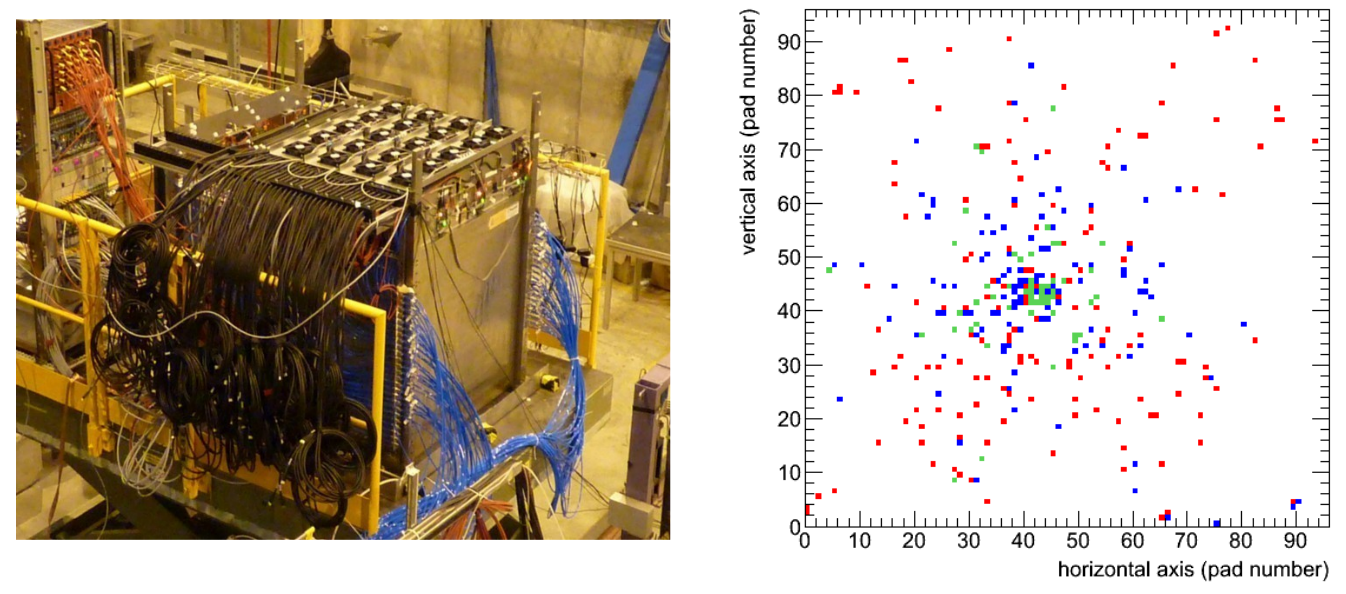
\includegraphics[width=0.95\textwidth]{Calorimeter/SDHCAL/test}
\caption{SDHCAL prototype in a beam line at the SPS at CERN (left). Event display of a 150\,GeV pion shower measured in a Micromegas prototype after 2\,$\lambda_{\rm int}$ of steel (right), the color indicates the threshold passed: red for 1, blue for 2 and green for 3.}
\label{sdhcal}
\end{centering}
\end{figure}


\subsubsection{The 1$\times$1\,m$^{2}$ Micromegas prototype}

\paragraph{Mechanics}
The Micromegas layers for the SDHCAL are made out of 6 high-voltage units installed together inside a gaseous chamber (Fig.\,\ref{mecha_elec} (right)). Each unit is an 8 layer PCB with a Bulk Micromegas mesh, readout pads and front-end ASICs; it is dubbed Active Sensor Unit (or ASU). A drift gap of 3\,mm is defined by spacers and a frame. Spacers are inserted in between ASUs, resulting in an inactive area of 2\,\%.


\begin{figure}
\begin{centering}
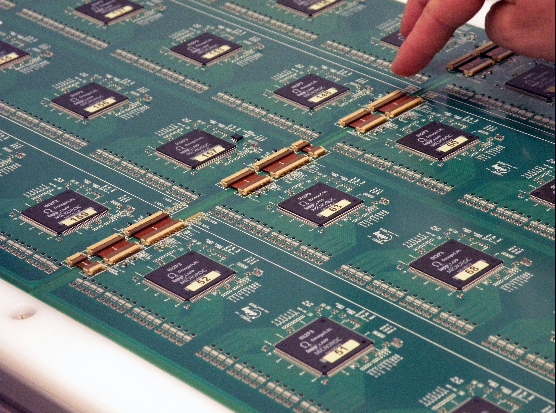
\includegraphics[width=0.45\textwidth]{Calorimeter/SDHCAL/intercon}
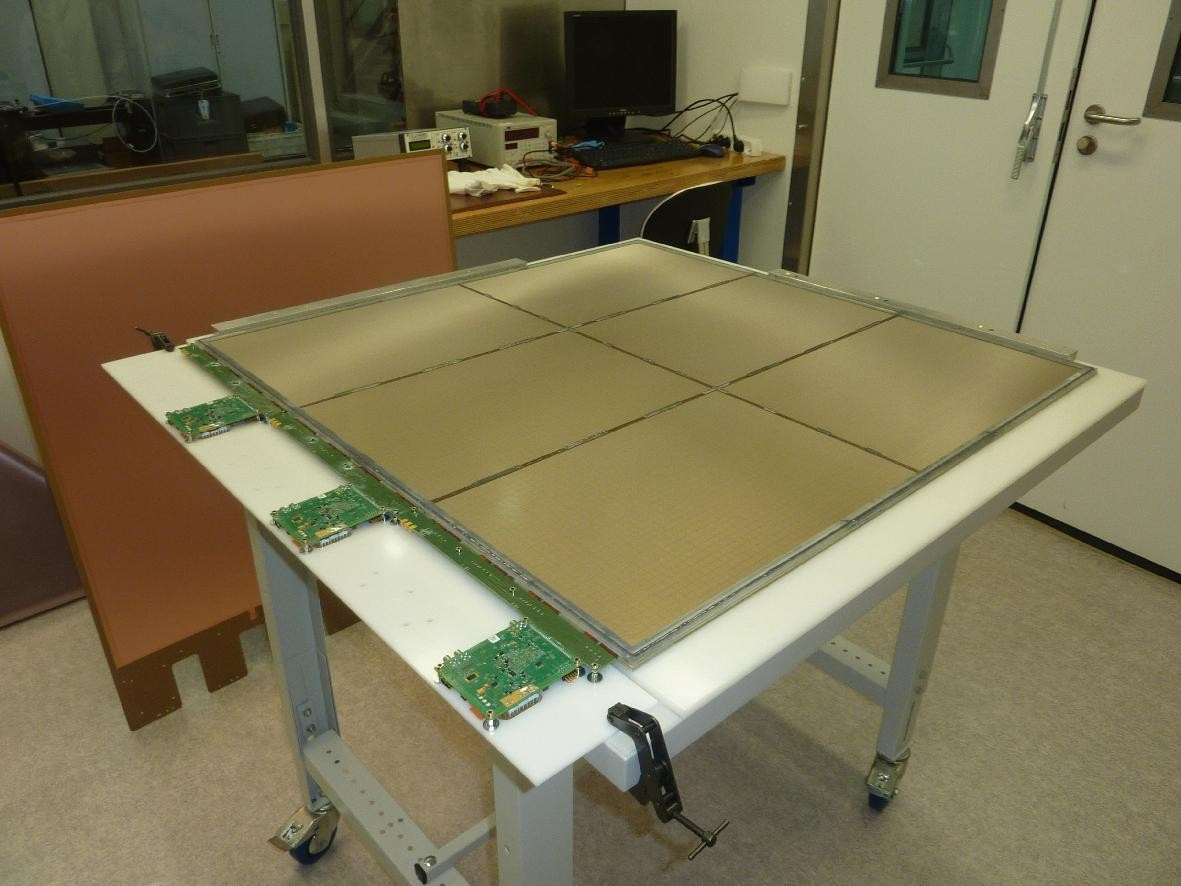
\includegraphics[width=0.45\textwidth]{Calorimeter/SDHCAL/m2_assembly}
\caption{Photographs of interconnections between 2 Active Sensor Units (left) and a 1$\times$1\,m$^{2}$ Micromegas prototype during assembly showing 6 of these units and a drift cover (right).}
\label{mecha_elec}
\end{centering}
\end{figure}


\paragraph{Electronics}
Electronics connections to the DAQ as well as services (power cables, gas pipes) are provided on one side of the prototype. ASU-to-ASU connections are therefore mandatory and are made with dedicated connectors and flexible cables (Fig.\,\ref{mecha_elec} (left)). They are used to distribute clocks and supply power to the ASICs, high voltage to the meshes, to configure the ASICs and read out data. Prior to assembly, 4 ASUs were chained and functional electronic tests were successfully performed. These key features make the design of the 1$\times$1\,m$^{2}$ Micromegas prototype fully scalable to the required size of a HCAL module at a future LC (at most 2\,m in the SiD detector concept).

\paragraph{Noise and detection efficiency}
A few prototypes were constructed~\cite{Adloff201390} and extensively tested in beam at CERN~\cite{Adloff:2014qea}. Noise conditions were excellent both during standalone tests and inside the CALICE SDHCAL. ASIC thresholds can be lowered down to about 20\,\% of a minimum ionising particle (MIP) signal at a typical running gas gain of 1500. Efficiency in excess of 95\,\% are easily reached while keeping a pad multiplicity below 1.1 for MIPs. The actual charge threshold is as low as 1--2\,fC; it is achieved on ASIC test-boards as well as once mounted on ASUs. The contribution of the PCB internal capacitances to the overall detector noise is therefore negligible.

\paragraph{Standalone performance}
Thanks to a precise control of the gas gaps and electronics settings, ASIC-to-ASIC variations of efficiency are below the percent in all tested prototypes. Although the statistics is low, the construction process seems reproducible. Stability with rate in high-energy hadron showers is excellent. Except occasional sparks, no effect of beam rate was observed on the pion response up to roughly 30 kHz beam rate; which was the highest rate during the tests. The measured spark probability lies in the range of 10$^{-6}$--10$^{-5}$ per showering pion at a running gas gain of 1500.

\subsubsection{Resistive prototypes}

While the Bulk Micromegas mesh is made of steel wires and is very resistant to sparking, sensitive front-end ASICs can suffer irreversible damage. Protections in the form of current-limiting diodes networks soldered on PCB were proved so far efficient. To simplify the PCB design and possibly reduce the overall detector cost, it is however desirable to get rid of diodes. It is well known that sparks can be suppressed by means of resistive coatings on the anode pad plane. This solution is used with great success in tracking detectors. Because it modifies the signal development, it needs some adaptation to calorimetry so as to preserve linearity and keep a narrow pad response function for Particle Flow reconstruction.


\begin{figure}
\begin{centering}
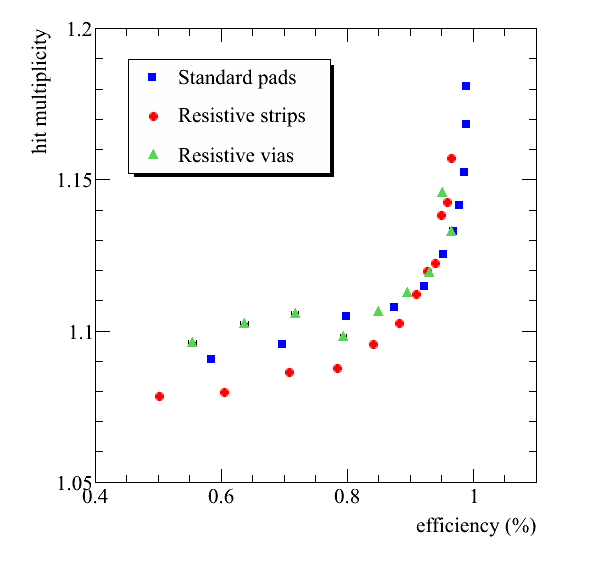
\includegraphics[width=0.45\textwidth]{Calorimeter/SDHCAL/splam_eff}
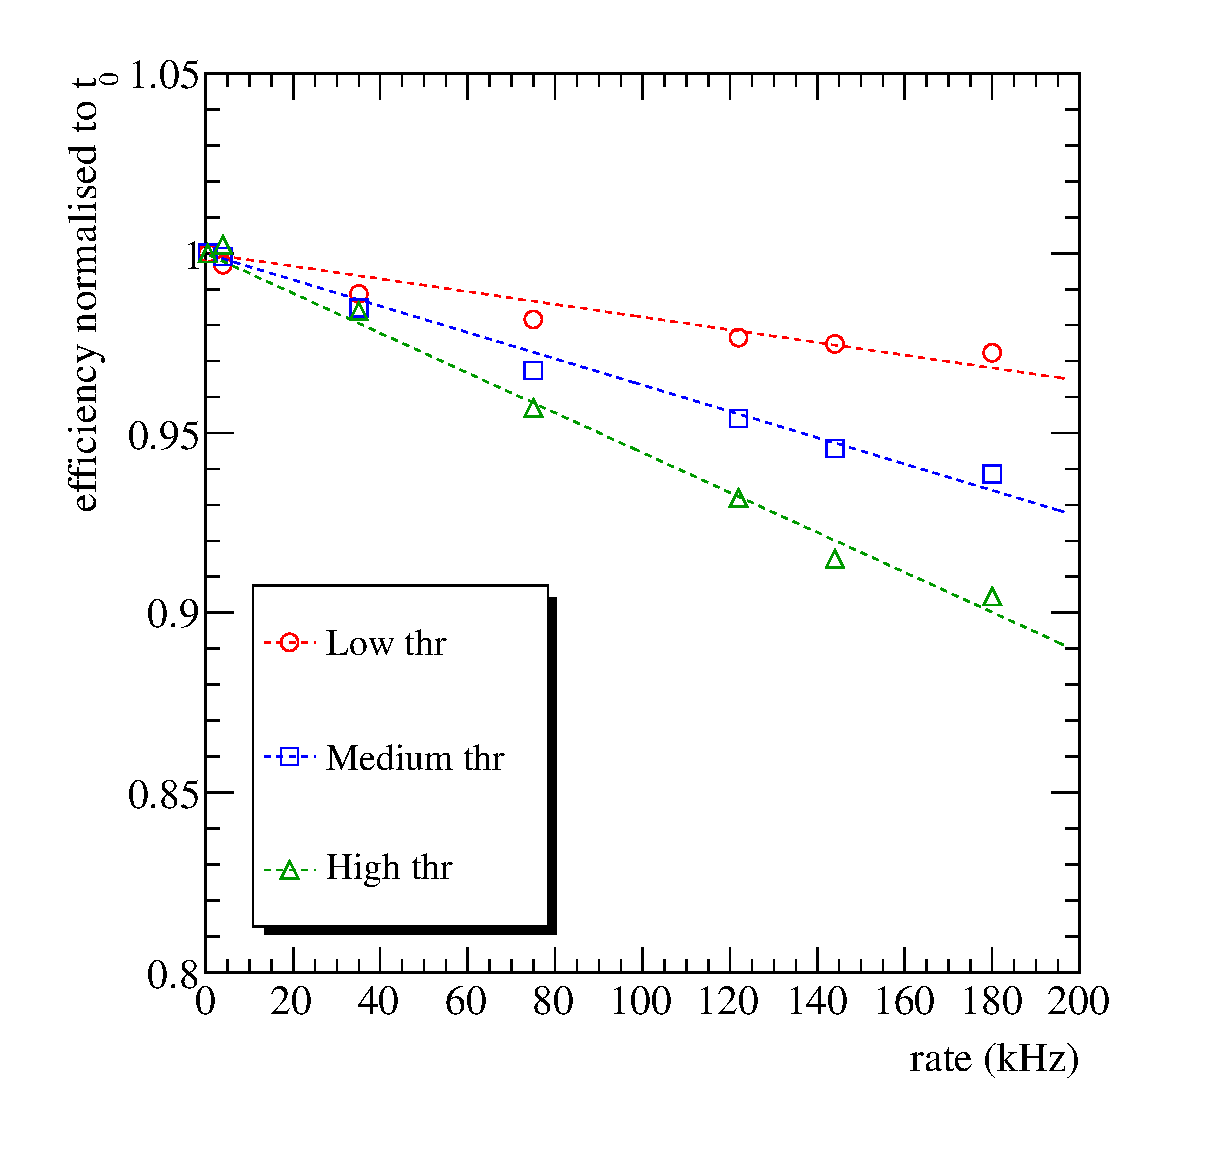
\includegraphics[width=0.45\textwidth]{Calorimeter/SDHCAL/splam_rate}
\caption{Pad multiplicity versus efficiency to 3\,GeV electrons for 2 resistive and 1 non-resistive (or standard) Micromegas prototypes (left). Efficiency dependence on rate in a resistive prototype for 3 values of threshold (right). The electron beam spot is $\sim$\,2$\times$2\,cm$^{2}$.}
\label{resistive}
\end{centering}
\end{figure}


First resistive designs using resistive strips and pads were implemented on small size prototypes. In a mixture of Ar/CO2, full suppression of sparking was demonstrated up to gas gain in excess of 10$^{4}$. At comparable gas gains, resistive and non-resistive prototypes show similar response to traversing charged particles, reaching high efficiency and low pad multiplicity. Compared to non-resistive ones, the evacuation of charge is slowed down in resistive prototypes which are thus subject to rate-dependent drops of gas gain. Expected efficiency losses have been observed at (3\,GeV electrons) rates in excess of 10\,kHz/cm$^{2}$. This limit is compatible with the resistivity of the coated material. At lower rates, it could be shown that the linearity of a Micromegas calorimeter to electrons is not affected by the resistive coatings, up to 5\,GeV, which was the maximum energy available during the testbeam campaign.

\subsection{Engineering Challenges}

\subsection{Future Plans}
Plans for the coming years include maintaining a commitment to linear collider detector R\&D and possibly seek new applications. Despite a decline of resources, an R\&D program to optimise resistive Micromegas for calorimetry is established. Linearity, rate capability and spark protection in dense electromagnetic showers will be checked up to high-energy and for detector designs with a large variety of resistivity and geometry. These measurements will be necessary to validate the resistive Micromegas technology for calorimetry at a future LC. Also, the on-going R\&D for high-luminosity LHC (HL-LHC) detector upgrades are an appealing perspective to the LAPP group. In particular, the possibility to equip the backing part of the CMS forward calorimeter is being investigated. Such high-rate application will put strong stability constraints on resistive Micromegas, making the optimisation work mentioned above even more relevant.

\begin{figure}
\begin{centering}
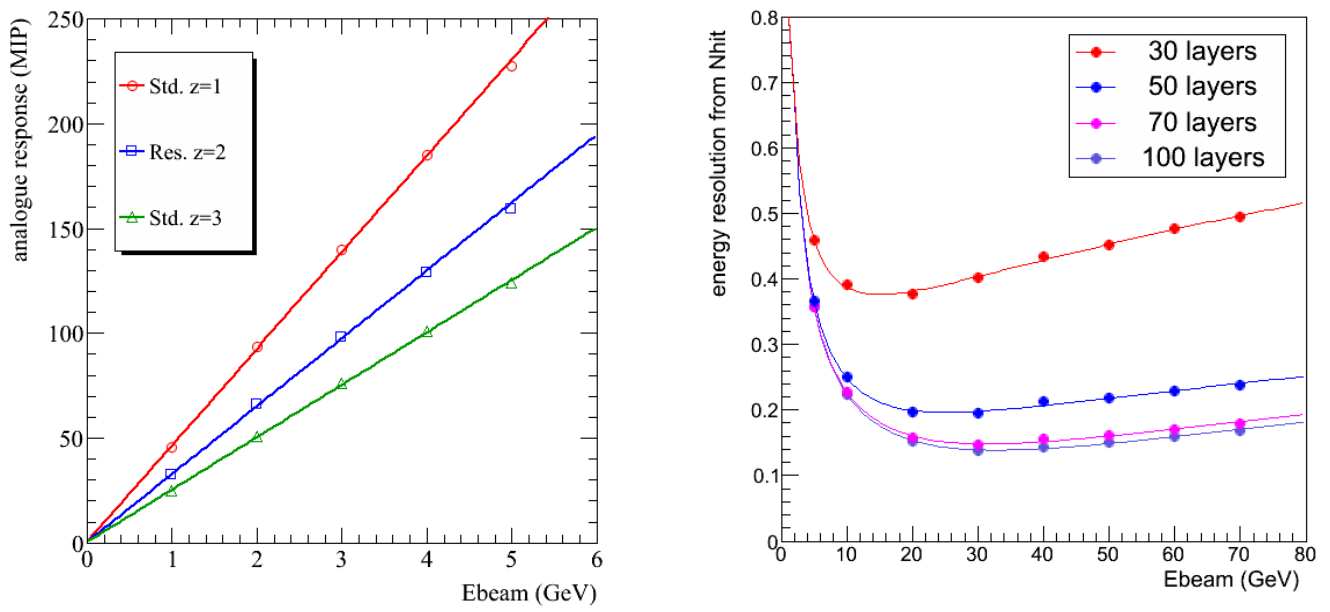
\includegraphics[width=0.8\textwidth]{Calorimeter/SDHCAL/test2}
\caption{Electron response of a virtual Micromegas SDHCAL deduced from measurements of longitudinal shower profiles in non-resistive (z=1 and z=3) and resistive (z=2) Micromegas prototypes placed behind increasing thicknesses of passive material (left). Geant4 calculation of the energy resolution to pions of a Micromegas DHCAL of 30 to 100 layers based on simple hit counting (right).}
\label{future}
\end{centering}
\end{figure}

On a longer term and if resources are sufficient, a Micromegas calorimeter prototype should be constructed so its performance can be compared to concurrent detector technologies. Some performance have already been studied with Monte Carlo simulation, the minimal prototype dimensions are known as well as its cost. This final step of the project naturally comes after optimisation of the resistive coating and would complete the R\&D on Micromegas calorimetry.

\subsection{Applications Outside of Linear Colliders}

\section{Glass RPC SDHCAL}
Contact person: Imad Laktineh (email: laktineh@IPNL.IN2P3.FR)
\subsection{Introduction}

Hadronic calorimeter (HCAL) plays an essential role in PFA-based experiments as
those proposed for the ILC. It allows to separate the deposits of charged and
neutral hadrons and to precisely measure the energy of the neutrals. The
contribution of the neutrals to the jet energy, around 10\% on average,
fluctuates in a wide range from event to event, and the accuracy of the
measurement is the dominant contribution to the particle flow resolution for jet
energies up to about \unit[100]{GeV}. For higher energies, the performance is
dominated by confusion, and both topological pattern recognition and energy
information are important for correct track cluster assignment.
High-granularity hadronic calorimeter is thus needed to achieve excellent jet
energy resolution.

HCAL proposed for both projects of ILC (ILD and SiD), are sampling calorimeters
with steel as absorber and scintillator tiles or gaseous devices with embedded
electronics for the active part. The steel was chosen due to its rigidity which
allows to build self-supporting structure without auxiliary supports (dead
regions). Moreover, the moderate ratio of hadronic interaction length
($\lambda_I = \unit[17]{cm}$) to electromagnetic radiation length ($X_0 = \unit[1.8]{cm}$) of
iron, allows a fine longitudinal sampling in terms of $X_0$ with a reasonable
number of layers in $\lambda_I$, thus keeping the detector volume and readout
channel count small. This fine sampling is beneficial both for the measurement
of the sizable electromagnetic energy part in hadronic showers as for the
topological resolution of shower substructure, needed for particle separation.

For the ILD project we propose gaseous detectors for the HCAL active layers: The
Resistive Plate Chamber (RPC). This is motivated by the excellent efficiency
and very good homogeneity the gaseous detectors could provide. Another
important advantage of gaseous detectors is the possibility to have very fine
lateral segmentation. Indeed, in contrast to scintillator tiles, the lateral
segmentation of gaseous devices is determined by the electronics readout used to
read them. Active layer thickness is also of importance for what concerns the
ILC hadronic calorimeter to be placed inside the magnetic field. Highly
efficient gaseous detectors can indeed be built with a thickness of less than
\unit[3]{mm}.

To obtain excellent resolution of hadronic shower energy measurement using a
binary readout, a lateral segmentation of few millimeters is needed. This
however leads to a huge number of electronics hardly affordable for the future
ILC hadronic calorimeters. $\unit[1\times 1]{cm^2}$ cells were found to be a good compromise
that still provides very good resolution at moderate energies. However,
simulation studies show that saturation effects are expected to show up at
higher energies ($> \unit[50]{GeV}$). This happens when many particles cross
one cell in the center of the hadronic shower. To reduce these effects, the
choice of multi-threshold electronics (Semi-Digital) readout was envisaged to
improve on the energy resolution by exploiting the particle density in more
appropriate way.

High-granularity calorimeters imply however a huge number of electronics
channels to operate them. This has two important consequences. The first is the
power consumption and the resulting increase of temperature which affects the
behavior of the active layers. The other consequence is the number of service
cables needed to power, read out these channels. These two aspects can
deteriorate the performance of the HCAL and destroy the principle of PFA if
they are not addressed properly.

The R\&D pursued by the SDHCAL-GRPC groups has succeeded to pass almost all the
technical hurdles of the PFA-based HCAL. The SDHCAL-GRPC groups have succeeded
to build the first technological prototype of these new-generation calorimeters
with 48 active layers of GRPC, $\unit[1]{m^2}$ each. The prototype validates the concept
of high-granularity gaseous detector and permits to study the energy resolution
of hadrons one can obtains with such calorimeter.


\subsection{Readout Electronics}

The readout electronics of the two Semi-Digital HCAL (SDHCAL) projects were
developed in common. An ASIC called HARDROC was first developed to read out the
GRPC detectors proposed for the ILD project. To solve the problem of
connections related to the high number of electronics channels, the option of a
detector embedded electronics using the DAISY chain scheme was chosen and
Printed Circuit Board (PCB) were conceived for the readout of large detectors
GRPC.

\subsubsection{Front-end ASIC}

The HARDROC chip (HR) implements a multi-threshold readout which integrates the
functionalities of amplification, shaping, digitization, internal triggering and
local storage of the data. Each of its 64 channels consists of a fast low
impedance current preamplifier with 8-bit variable gain (in the $[0,2]$ range)
followed by 3 fast shapers (\unit[15]{ns} shaping time). A low offset discriminator is
present on each path and the three corresponding thresholds establish the
multi-level readout. The thresholds are set using three integrated 10-bit
Digital to Analog Converters (DAC). The outputs of the three discriminators are
then encoded 3-to-2 bit and stored in an internal digital memory latched by a
trigger event.

A trigger is generated when one of the lowest level discriminators is fired but
can also be configured on the other thresholds. A frame consists of the 64
encoded discriminator outputs, plus a 24-bit time-stamp and a chip identifier is
stored after a trigger is received. Noisy channels could be easily masked via
the configuration parameters control. In order to avoid fake triggers produced
by noisy channels, the output of each discriminator can be switched off from the
trigger generator logic via the configuration parameters control (Slow Control
hereafter) commands. The response of all the channels can be calibrated by
injecting an analog signal through an integrated $\unit[2\pm 0.02]{pF}$ input test
capacitor; this is a useful tool to make the response of the different channels
as uniform as possible~\cite{1748-0221-6-02-P02001}.

The ASIC contains a 127-frame long digital memory. This allows to work in a
triggerless mode and keep all the data accumulated during the bench crossing.
Once the memory is full the acquisition is stopped, the readout is performed
and the ASIC can start acquisition again. The Gray-coded time-stamp is derived
from an external \unit[5]{MHz} clock.

An essential feature of the HR is the possibility to be operated in the
power-pulsing mode (PP) that consists of switching off almost all
power-consumption functionalities in between the bench crossings (BC) of the ILC
electron beams. With the ILC duty cycle of one \unit[1]{ms} of BC every \unit[200]{ms}, this
mode allows a reduction factor of more than 100 of power consumption. Thanks to
this reduction, the temperature increase of the HCAL is moderate and only
simple cooling system is needed to operate it efficiently.

\subsubsection{Active Sensor Units}

To read out the $\unit[1]{m^2}$ detector of the SDHCAL, an electronic board with the
same size is needed. This electronic board is an important piece in the present
design. It hosts both the pick-up pads and the ASICs in addition to the
connections linking the pads to the ASICs and those among the different ASICs.
To ensure good transmission qualities and low cross-talk, 8-layer Printed
Circuit Board (PCB) is designed. Feasibility constraints, make the tasks of
circuit production, components soldering, testing and handling of the
assemblies, exceedingly difficult in the case of a single board of one square
meter. The solution of dividing that circuit into 6 smaller but more
manageable PCB was adopted. Each of these small ASUs hosts 24 chips to read out
$48\times 32$ pads of $\unit[1]{cm^2}$ each. This dressed PCB is dubbed Active Sensor
Unit (ASU). The base pattern connecting 64 pads arranged in a $8\times 8$ matrix
to the ASIC's pins is shown in Figure~\ref{fig:Calorimeter:SDHCAL_GRPC:asicPins}. This is identical to the
one used in the ASUs of the small GRPC chambers described in reference
\cite{1748-0221-6-02-P02001}. The routing of each input signal from its own pad up to chip pin
has been carefully optimized to reduce the cross-talk. All input signals are
laid out in the same analog signal layer witch is sandwiched between two GND
layers. The routing of digital signals was kept well separated from the vias
connecting signals from one layer to another. In the case of the GRPC related
ASU, the HARDROC base pattern is replicated $4\times 6$ times in the $\unit[33.33]{cm}
\times \unit[50]{cm}$ board. 4 \unit[1.6]{mm} diameter holes are present on the four
angles of a PCB to be used for fixation purposes as will be explained later.
The rooting was conceived so two of the ASUs can be associated to form one slab
hosting 48 ASICS. Each slab is then connected to one Detector InterFace board
(DIF). The connection between the DIF and the slab as well as the connection
of the two ASUs is performed thanks to tiny connectors allowing the
different clocks, signals as well as the power to circulate between the two
ASUs. Three slabs are then assembled to form the required electronics board.
To ensure the same electric reference level for the six ASUs, the GND layer of
the six ASUs is connected thanks to a copper gasket on all the common sides.
Similar schemes could be proposed for GRPC detectors with larger size.


\begin{figure}
\centering
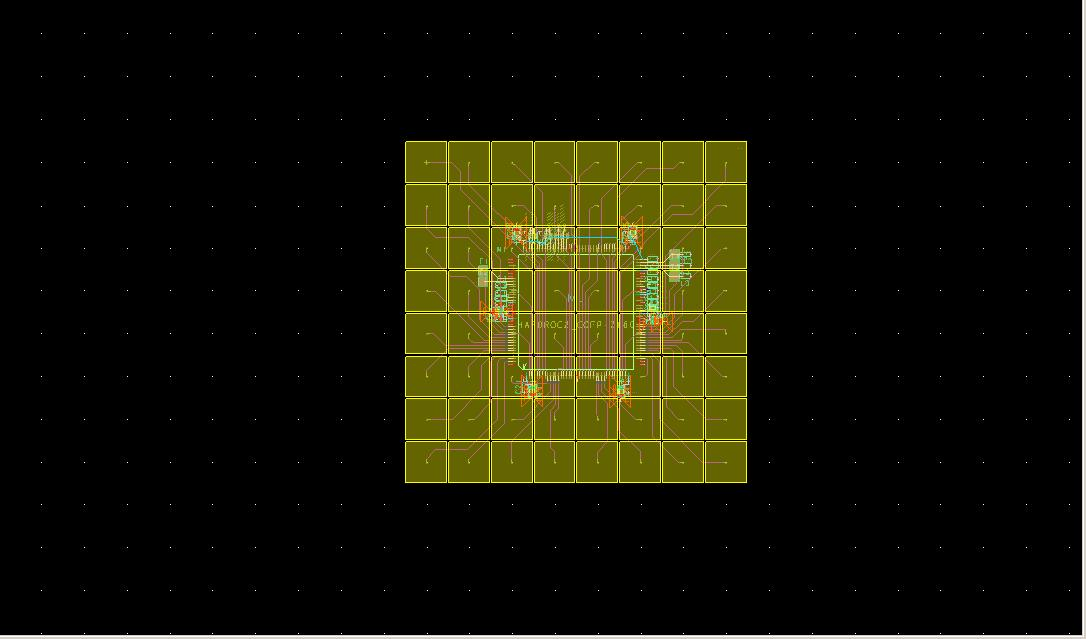
\includegraphics[width=.7\columnwidth]{Calorimeter/SDHCAL_GRPC/figures/HR2_base.jpg}
\caption{Pads connection to the ASIC's pins}
\label{fig:Calorimeter:SDHCAL_GRPC:asicPins}
\end{figure}


\subsubsection{Front-end and back-end boards}

The interface between the ASUs and the data acquisition system (DAQ) is realised
by the detector interface board called DIF. The main elements of the DIF is an
FPGA and USB, HDMI and SAMTEC connectors. It manages the control signals
(e.g. clock, busy/ready, external/internal trigger, power-pulsing) and
supply power to the ASICs and also performs the readout of the ASIC memories.
DIFs are read out by other FPGA-based boards called Data Concentrator Cards
(DCC). They can be connected up to 9 DIFs through HDMI links and are controlled
by a synchronous DCC (or SDCC). The SDCC can connects to up to 9 DCCs to which
it distributes the clock and the commands. It is also connected to the computer
network for the user to control the DAQ.

In the case of Micromegas ASUs, a small additional board called inter-DIF is
used between the DIF and ASU to provide the high voltage to the meshes and drift
electrode.


\subsubsection{Acquisition Software}

To exploit the data collected by the SDHCAL detectors an acquisition software
was developed. This software is organized in three parts. The first one allows
to access the hardware devices (DIF, SDCC) through an FTDI chip associated to
each of these devices. It transmits the configurations parameters to ASICs
through these devices and collect the data as well. The second part is the
configuration data base. It gives the possibility to store and retrieve all
parameters needed by the DAQ system. The database itself is hosted on an Oracle
server at CC IN2P3 (Villeurbanne, France). To interface this SQL database with
the DAQ software and to allow users to insert and query data without knowledge
of SQL, a C++ library has been written. A special care was taken to allow to
download the parameters associated to a given parameters of the prototype
(roughly 550000 parameters) in few seconds. The third part concerns the data
collection. Data from different DIFs may be readout at a different times but
will have the same Bench Crossing IDentifier (BCID) for a given trigger. The
logical way to keep synchronicity is to store in a BCID indexed map the buffers
of all read DIFs but it requires to man-age memory allocation, access and
cleaning. This was achieved thanks to the abilities offered by recent Linux
kernels to use file based shared memory. In addition, whenever several
computers are involved in the data taking, as it is the case for the SDHCAL
prototype, a communication framework is needed. The CMS data acquisition XDAQ
framework was chosen. This provides communication tools with both binary and
XML, an XML description of the computer and software architecture, a web-server
implementation of all data acquisition application and a scalable event builder.
A monitoring system was also developed to have a online follow-up of the
acquisition during data collection.

\subsection{GRPC-SDHCAL for ILD}
\subsubsection{Detector Development}

The structure
of GRPC proposed as an active layer of the HCAL proposed for ILD is shown in
Figure~\ref{fig:Calorimeter:SDHCAL_GRPC:chamber}. It is made out of two glass plates of \unit[0.7]{mm} and \unit[1.1]{mm}
thickness. The thinner is used to form the anode while the the thicker forms
the cathode. Ceramic balls of \unit[1.2]{mm} diameter are used as spacers between the
glass plates. The balls are glued on only one of the glass plates. In
addition to those balls, 13 cylindrical fiber-glass buttons of \unit[4]{mm} diameter
are also used. Contrary to the ceramic balls the buttons are glued to both
plates ensuring thus a robust structure.

Special spacers (ceramic balls) were used to maintain uniform gas gap of \unit[1.2]{mm}.
Their number and distribution were optimized to reduce the noise and dead
zones ($0.1 \%$). The distance between the spacers (\unit[10]{cm}) was fixed so that
the deviation of the gap distance between the two plates under the glass weight
and the electric force does not exceed \unit[45]{microns}. The choice of these spacers
rather than fishing lines was intended to reduce the dead zones ($0.1 \%$). It
was also aimed at reducing the noise contribution observed along the fishing
lines in standard GRPC chambers. The gas volume is closed by a \unit[1.2]{mm} thicks
and \unit[3]{mm} wide glass-fiber frame glued on both glass plates. The glue used for
both the frame and the spacers was chosen for its chemical passivity and long
term performance.

The resistive coating on the glass plates which is used to apply the high
voltage and thus to create the electric field in the gas volume was found to
play important role in the pad multiplicity associated to a mip \cite{1748-0221-6-02-P02001}.
To find the best coating for GRPC chambers many products were tested. Finally, a
new product based on two components was chosen. By changing the two components
ration one can obtain the needed surface resistivity. Commercial products like
Licron\texttrademark and Statguard\texttrademark which are used for Electro-Static
Discharge (ESD) applications were tried and few $\unit[1]{m^2}$ chambers were built
using those products and intensively tested. Both products failed to satisfy our
application either for long term stability under the high voltage (Licronusing
those products ) or due to the impossibility to obtain the surface uniformity
needed for our application (Statguardusing those products ). Eventually, two
products were identified, both of which are based on colloids containing
graphite. Both can be applied using the silk screen print method, which ensures
very uniform surface quality. One of these products is a single component paint
with a dry surface resistivity of $\unit[1-10] M\Omega/\square$. The second product
comes as two components which must be mixed by the user. The surface resistivity
may be adjusted over a wide range by changing the mix ratio. Both products
require baking at around $170^\circ$ C to attain a stable surface resistivity.
One product based on colloids containing graphite was finally selected. The
product can be applied using the silk screen print method, which ensures very
uniform surface quality. In addition, the product is made of two components and
it was found that by changing the mix ratio the surface resistivity may be
adjusted over a wide range.

The measured surface resistivity at various points over a $\unit[1]{m^2}$ glass coated
with the previous paint showed a mean value of $\unit[1.2]{M\Omega/\square}$ and a
ratio of the maximum to minimum values of less than 2. A study was also made of
the repeatability of the surface resistivity between different mix batches. It
was found that surface resistivity in the range $\unit[0.5-2]{M\Omega/\square}$ could be
reliably reproduced. For $\unit[1]{m^2}$ GRPCs the painting is applied on the whole
glass plate except for \unit[3]{mm} from the edges. This distance, corresponding to the
frame width, was optimized so the dead zone of the detector is reduced while
external sparks due to the presence of the metallic cassette in the vicinity is
completely eliminated.

Another important aspect of this development concerns the gas circulation within
the GRPC taking into account that for ILD SDHCAL gas outlets should all be on
one side. A genuine system was proposed. It is based on channeling the gas
along one side of the chamber and releasing it into the main gas volume at
regular intervals. A similar system is used to collect the gas on the opposite
side. A finite element model has been established to check the gas
distribution~\cite{Bedjidian2010120}. The simulation confirms that the gas speed is
reasonably uniform over most of the chamber area.


In order to improve on the gas distribution in large chambers taking into
account the requirement that both gas outlets should be on the same side of the
detector to satisfy all possible mechanical structures proposed for ILD
hadronic calorimeter, new schemes were studied. The one we finally adopted
allows us to improve the gas distribution by channeling the gas along one side
of the chamber and releasing it into the main gas volume at regular intervals
thanks to \unit[1.2]{mm} diameter PEEK\texttrademark tubes fixed \unit[2]{cm} from the
chamber side. A similar system is used to collect the gas at the other side of
the chamber. A finite element model has been established to check the gas
distribution~\cite{Bedjidian2010120}. The simulation confirms that the gas speed is
reasonably uniform over most of the chamber area. as can be seen in
Figure~\ref{fig:Calorimeter:SDHCAL_GRPC:gas_distribution}.

The GRPC and its associated electronics are housed in a special cassette which
protects the chamber and ensures that the readout board is in intimate contact
with the anode glass. The cassette is a thin box consisting of \unit[2.5]{mm} thick
stainless steel plates separated by \unit[6]{mm} wide stainless steel spacers. Its
plates are also a part of the absorber.

The electronics board is assembled thanks to a polycarbonate spacer which is
also used to fill the gaps between the readout chips and to improve the overall
rigidity of the detector. The electronics board is fixed on the small plate of
the cassette. Thanks to tiny screws and the new set is fixed on the other plate
which hosts the detector and the spacers. The whole width of the cassette is \unit[11]{mm}
with only 6 of them corresponding to the sensitive medium including the GRPC
detector and the readout electronics.


\begin{figure}
\centering
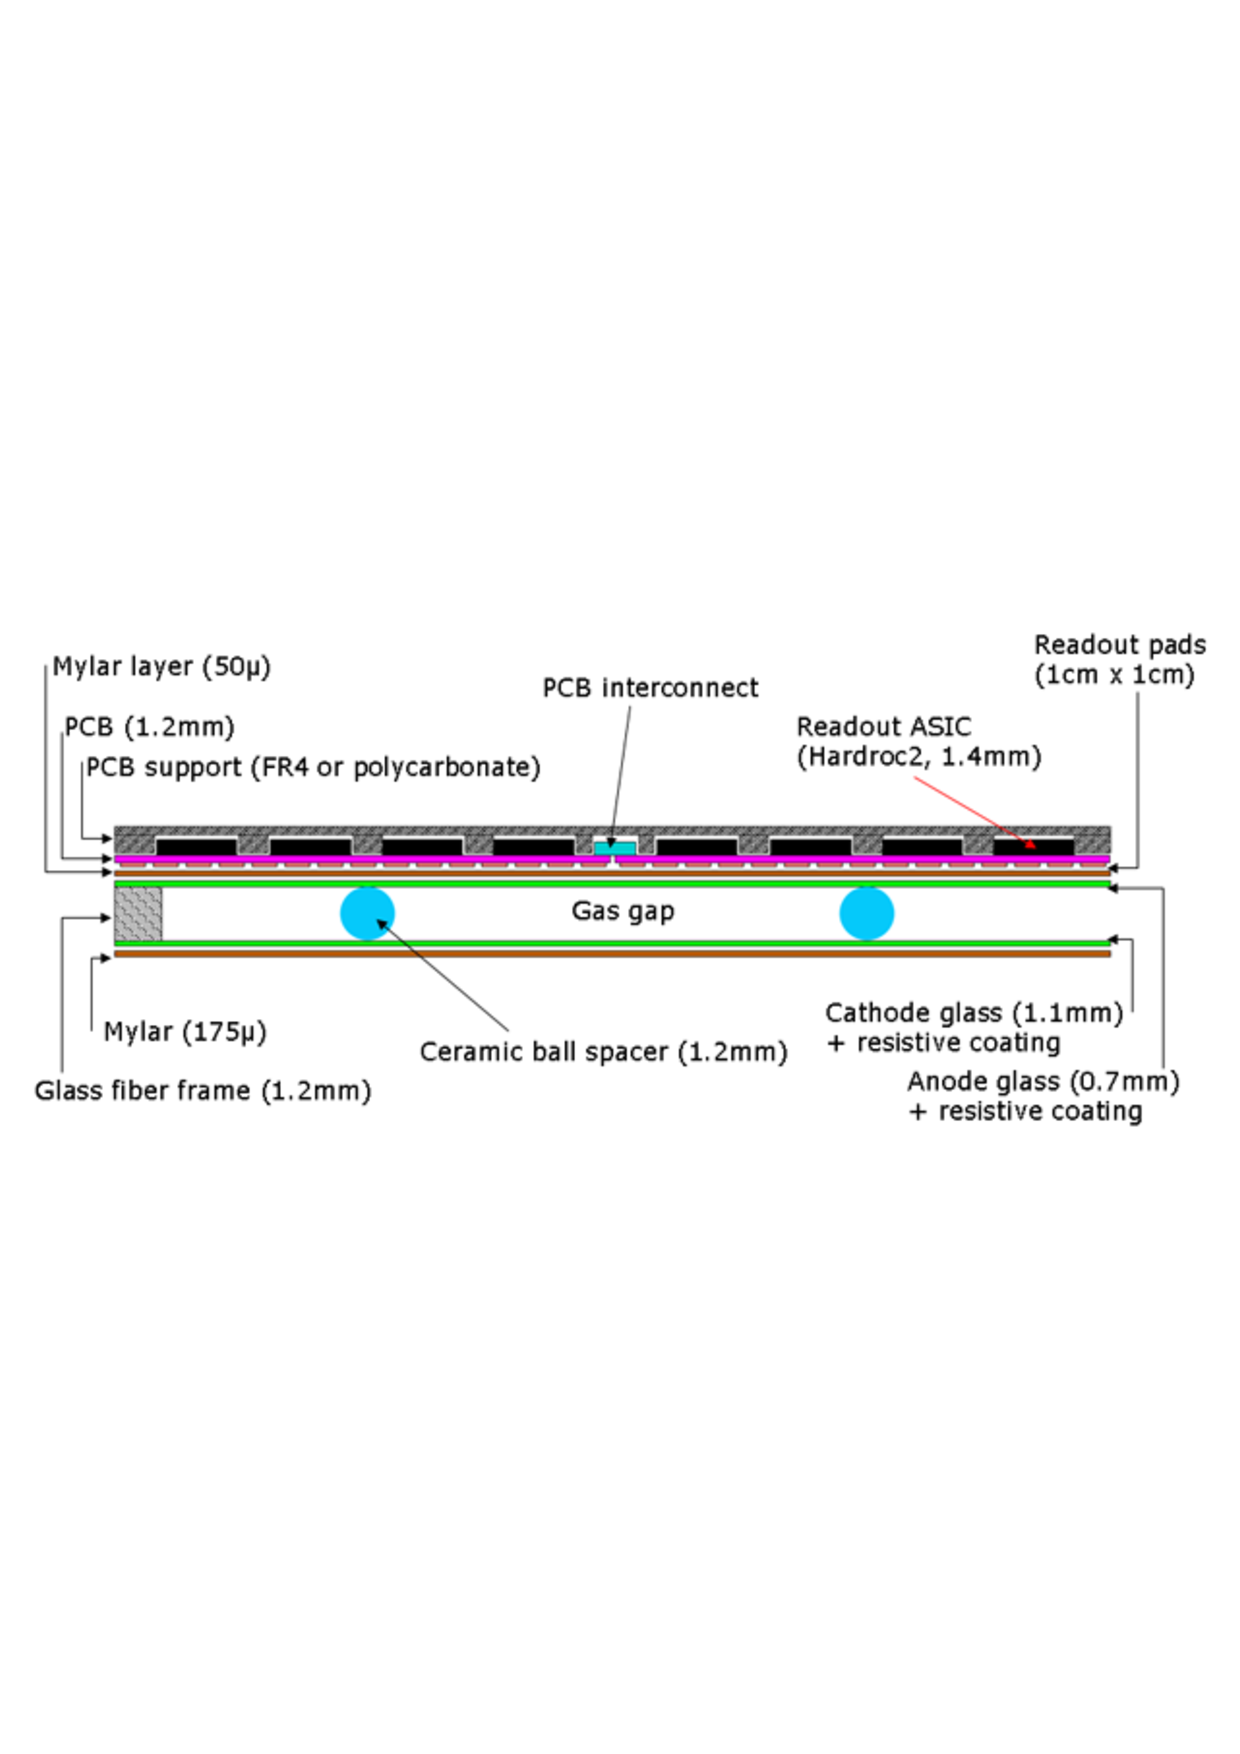
\includegraphics[width=0.70\textwidth]{Calorimeter/SDHCAL_GRPC/figures/chamber}
\caption{Cross-section through a $\unit[1]{m^2}$ chamber}
\label{fig:Calorimeter:SDHCAL_GRPC:chamber}
\end{figure}


\begin{figure}
\centering
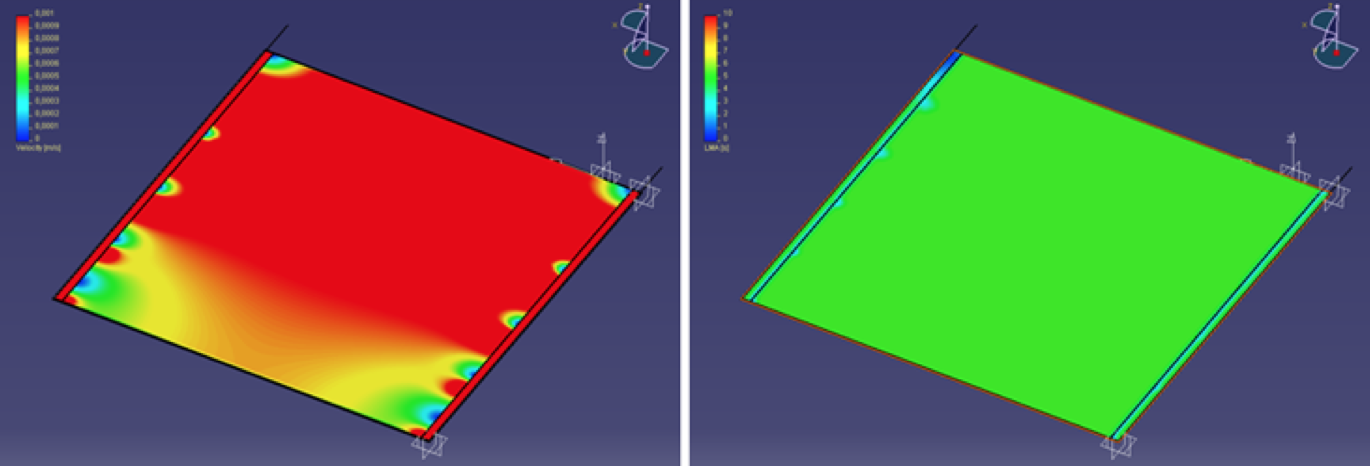
\includegraphics[width=.9\textwidth]{Calorimeter/SDHCAL_GRPC/figures/gas.png}
\caption{Left: Gas speed profile in the range \unit[0--1]{mm/s}; Right: Least mean age profile in the range \unit[0--10]{s}}
\label{fig:Calorimeter:SDHCAL_GRPC:gas_distribution}
\end{figure}

\subsection{Prototype}

A technological prototype corresponding to the SDHCAL option proposed in the ILC
LOI was built. 48 cassettes as the one described above were built. They
fulfilled a stringent quality control. It is worth mentioning that 10500 HR
ASICs were produced and tested using a dedicated robot for this purpose. The
yield was found to be higher than 92\%. The ASICs were then fixed on the PCBs
to make a $\unit[1]{m^2}$ and itself fixed on the cassette cover once successfully
tested.

The cassettes were inserted in a self-supporting mechanical structure that was
conceived and built in collaboration with the Spanish group of CIEMAT. The
structure is made of Stainless Steel plates of \unit[1.5]{cm} each. The plates were
machined to have an excellent flatness and well controlled thickness. The
flatness of the plates was measured using a laser-based interferometer system.
It was found that the flatness of the plates are less than 500 microns. This
results guarantees that for the SDHCAL V structure proposed for ILD, a tolerance
of less than \unit[1]{mm} is achievable.

The first cassettes were extensively tested using a cosmic-rays bench and later
particles beam at CERN. Both the efficiency and the multiplicity of the GRPC
cassettes were studied. These studies showed high efficiency and good
homogeneity and validated the cassette concept.

The prototype construction lasted less than 6 months. A commissioning test at
CERN in 2011 allowed to understand the whole system behavior. More precisely a
problem related to the acquisition system of the more than 430000 channels was
found and fixed.

In parallel a single cassette was tested in a magnetic field of 3 Tesla (H2 line
at CERN) applying the power-pulsed mode. The TB results indicated clearly that
the use of the power-pulsed mode in such a magnetic field is possible. The
behavior of the detector (efficiency, Figure~\ref{fig:Calorimeter:SDHCAL_GRPC:Eff}, multiplicity, Figure~\ref{fig:Calorimeter:SDHCAL_GRPC:Mult}) was found to be similar to
those obtained in the absence of both the magnetic field and the power-pulsed
mode.

In April 2012 the prototype was exposed to pion, muon, electron beams of both
the PS and the SPS of CERN (Figure~\ref{fig:Calorimeter:SDHCAL_GRPC:prototype}). Power-pulsed mode was applied to the
whole prototype using the beam cycle structure (\unit[0.3]{ms} time duration for the PS
beam and \unit[9]{s} for the SPS beam every \unit[45]{s}). A basic water-based cooling system was
used to keep under control the temperature increase particularly in in the case
of the SPS where the consumption reduction is only 5 (to compare with a factor
of more than 100 in the ILC case). An acquisition mode simliar to that of the ILC was operated.
The data were collected continuously in a triggerless mode. The DAQ stops when
the memory of one ASIC is full. Data are then transferred to a storage station
and then the acquisition starts again. Figures~\ref{fig:Calorimeter:SDHCAL_GRPC:PP1} and \ref{fig:Calorimeter:SDHCAL_GRPC:PP2} show the efficiency and
pad multiplicity of the prototype GRPC chambers measured using the muon beam.

The SDHCAL prototype results obtained with a minimum data treatment (no grain
correction) show clearly that excellent linearity and good resolution could be
achieved on large energy scale as can be shown in Figures~\ref{fig:Calorimeter:SDHCAL_GRPC:Linearity} and ~\ref{fig:Calorimeter:SDHCAL_GRPC:Resolution}. Useless to
mention that the high granularity of the SDHCAL allows one to study thoroughly
the hadronic showers topology and to improve on the energy resolution by, among
others, separating the electromagnetic and the hadronic contribution. The
separation between close-by showers will also get big benefit thanks to the high
granularity on the one hand and to to the very clean detector response ( $< \unit[1]{Hz/cm^2}$ )
on the other hand. These two points are being worked and recent results confirm this.

The quality of data obtained during three weeks of data taking validates
completely the SDHCAL concept as proposed in the LOI. This is especially
encouraging since no gain correction was applied to the electronics channels to
equalize their response. However a gain correction mode is elaborated and tested
during the TB. It will be applied in the future to assess the effect of such
correction on the energy resolution.


\subsection{ILD Preparation}

The expertise acquired with the construction and
the commissioning of the technological prototype and the obtained results were
used to implement a realistic simulation of the ILD HCAL. Physics channels such
as the $\mathrm{t} \bar{\mathrm{t}}\mathrm{H}$ were studied using the SDHCAL option and results were found
identical to those obtained with the scintillator tile option despite the fact
that the jet energy reconstruction code was optimized for the latter.

In addition, the French groups participated actively in the HCAL part of the
ILC TDR (ILD part) by proposing a genuine mechanical structure for the hadronic
calorimeter (called V-structure). The V structure was conceived to eliminate
the projective holes and cracks so none of the particles produced close to the
detector centre could escape detection. The V structure has additional
advantages. It eliminates in principle the space between the barrel and the
Endcaps avoiding the shower deformation which results not only because of
this space but also of the different cables and services needed in CMS-like
mechanical structures. In this structure the different services such as the
gas tubes, data collection and electric cables of both the barrel and the
Endcaps are taken out from the outer radius side.Detailed studies have shown
that the deformation of this structure is extremely low and its robustness was
verified experimentally with the SDHCAL technological prototype built with a
self-supporting structure respecting the spirit of the V one. Services and
Integration issues were also worked out. Besides, realistic costing was
performed , based on the prototype experience.

\begin{figure}
\centering
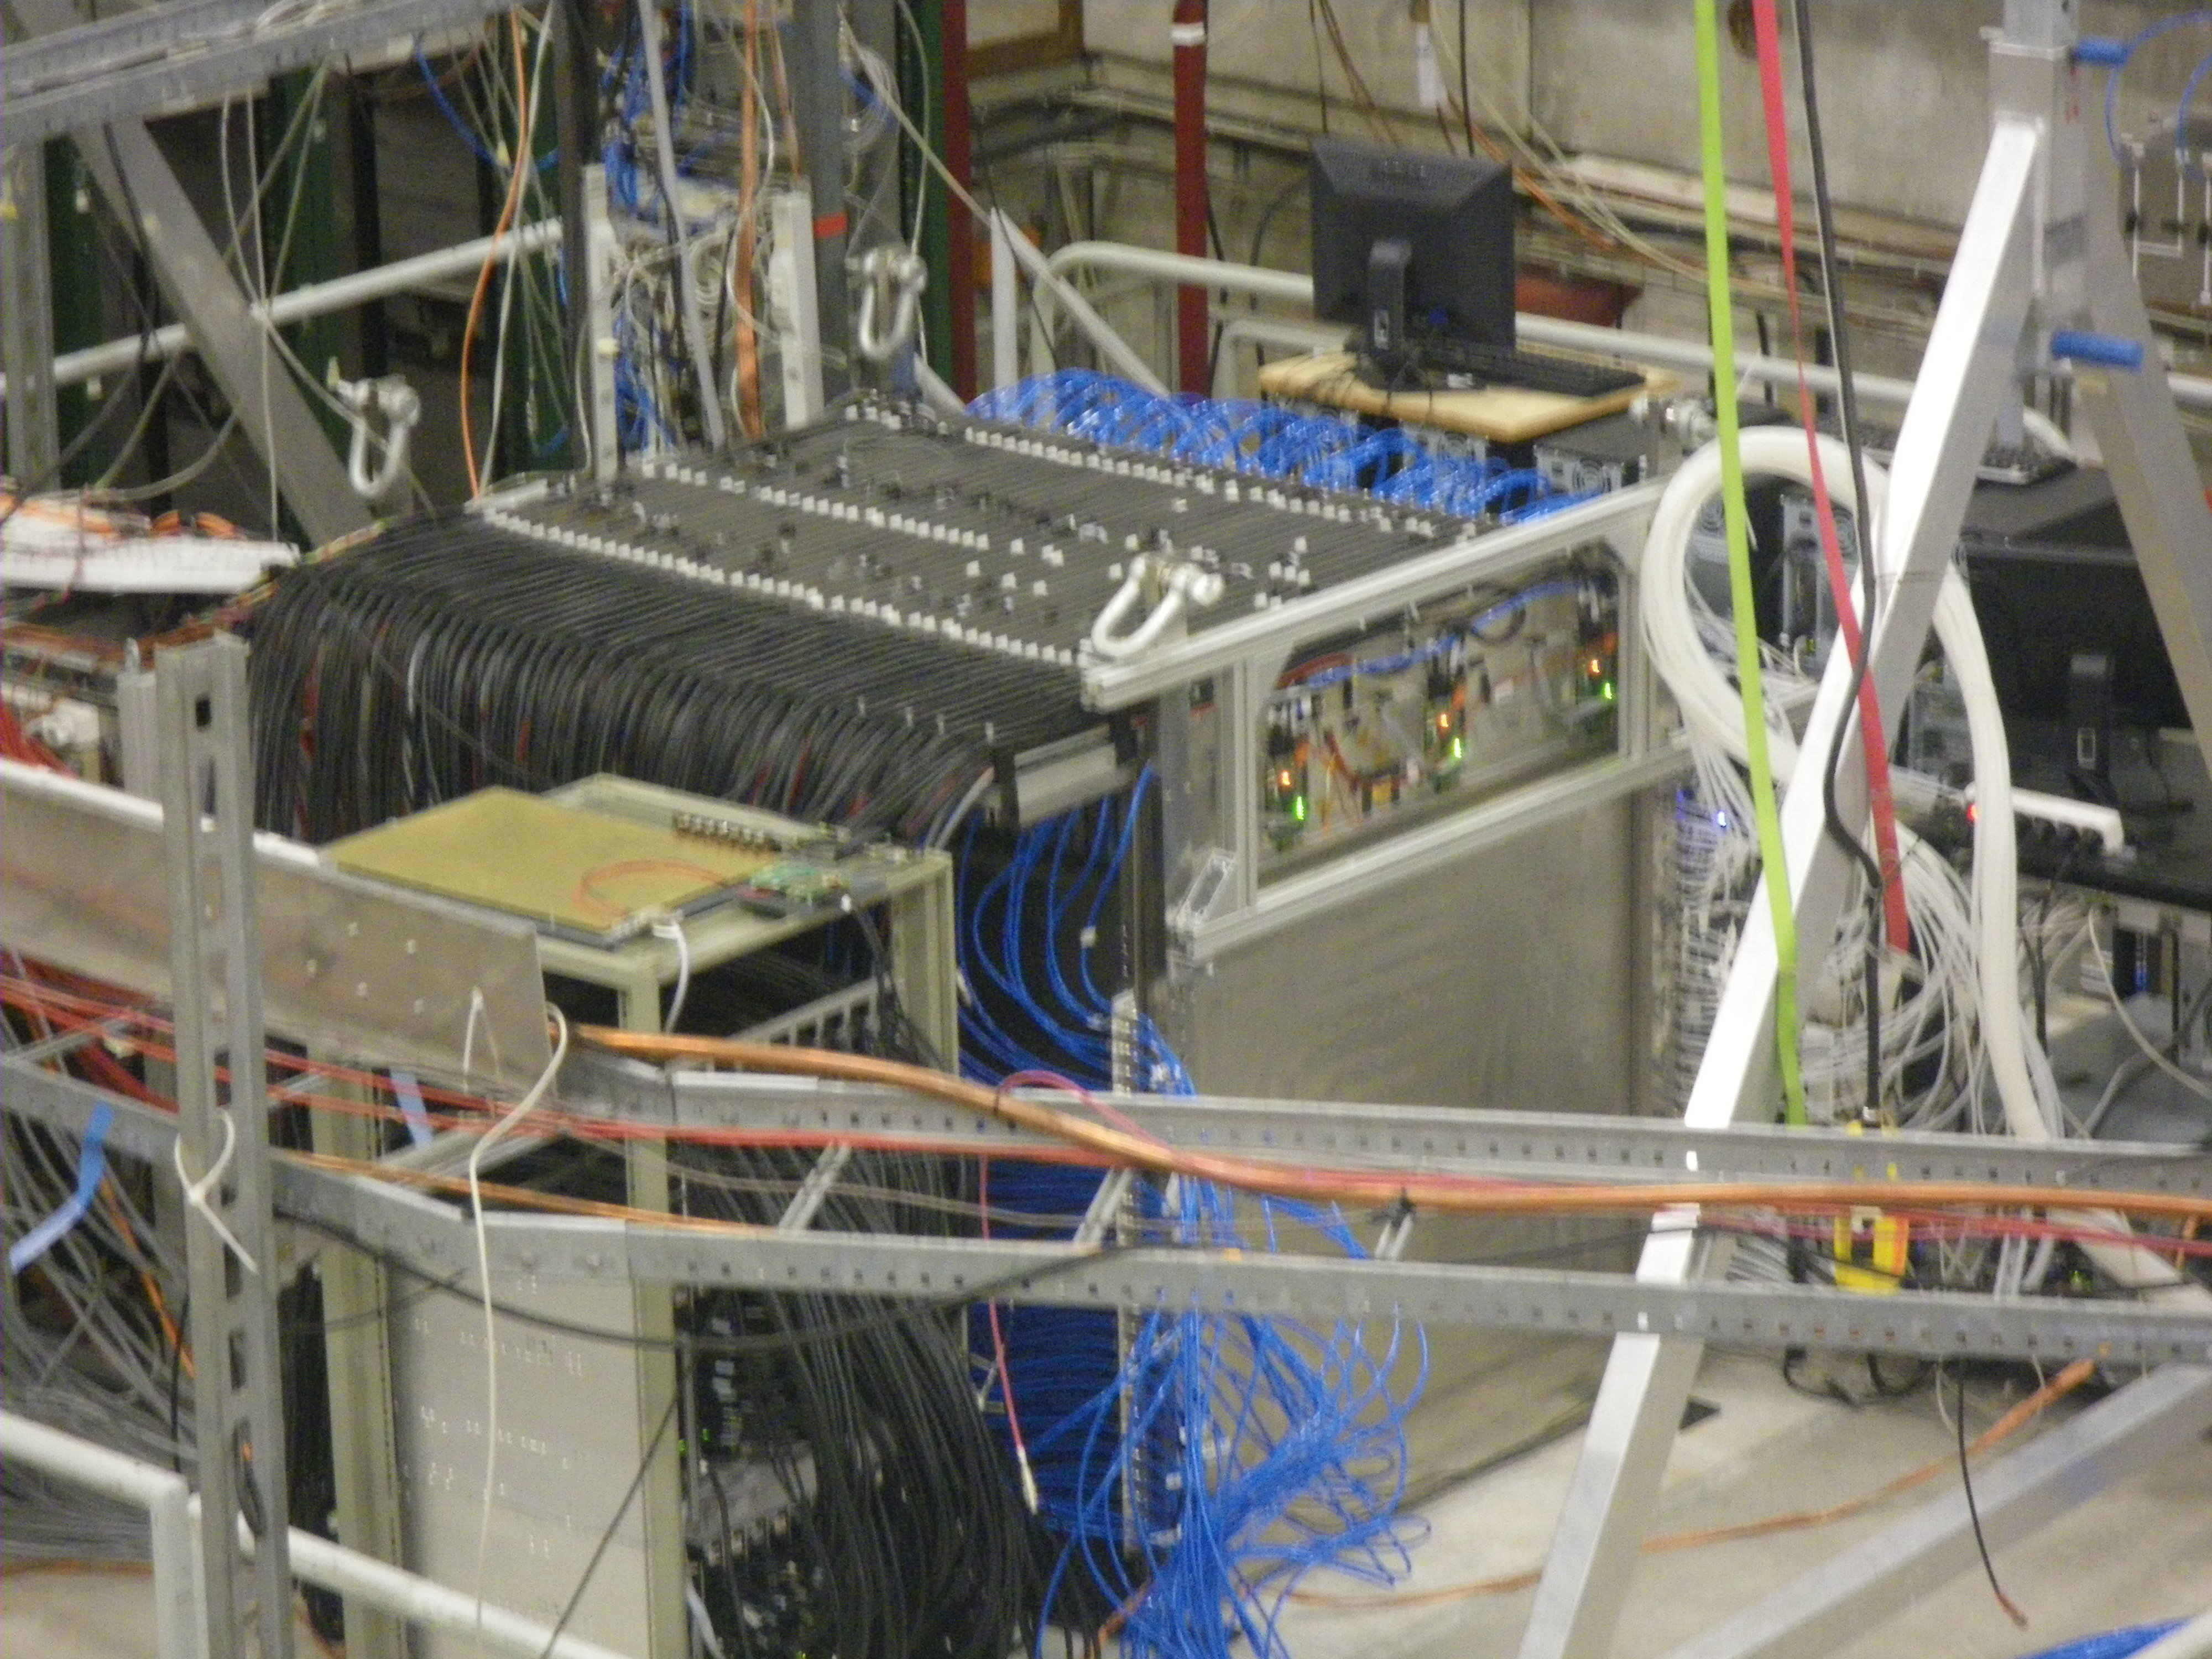
\includegraphics[width=0.50\columnwidth]{Calorimeter/SDHCAL_GRPC/figures/prototype.JPG}
\caption{Cross-section through a $\unit[1]{m^2}$ chamber.}
\label{fig:Calorimeter:SDHCAL_GRPC:prototype}
\end{figure}

\begin{figure}
\centering
 \begin{minipage}[t]{0.49\textwidth}
 \includegraphics*[width=\textwidth,keepaspectratio]{Calorimeter/SDHCAL_GRPC/figures/eff_layer_august_fit.pdf}
	\caption{Efficiency of the GRPC protoype}
 \label{fig:Calorimeter:SDHCAL_GRPC:Eff}
 \end{minipage}
\hfill
 \begin{minipage}[t]{0.49\textwidth}
 \includegraphics*[width=\textwidth,keepaspectratio]{Calorimeter/SDHCAL_GRPC/figures/mul_layer_august_fit.pdf}
 \caption{Pad multiplicity of the GRPC prototype. }
 \label{fig:Calorimeter:SDHCAL_GRPC:Mult}
 \end{minipage}
 \end{figure}

\begin{figure}
    \centering
 \begin{minipage}[t]{0.45\textwidth}
 \includegraphics*[width=0.7\textwidth,keepaspectratio]{Calorimeter/SDHCAL_GRPC/figures/BeamLine.jpg}
	\caption{GRPC setup in the CERN SPS-H2 line magnetic field.}
 \label{fig:Calorimeter:SDHCAL_GRPC:PP1}
 \end{minipage}
 \hfill
 \begin{minipage}[t]{0.45\textwidth}
 \includegraphics*[width=\textwidth,keepaspectratio]{Calorimeter/SDHCAL_GRPC/figures/BField_Efficiency_PowerPulsed.pdf}
 \caption{Efficiency scan over high voltage, with and without power pulsing. }
 \label{fig:Calorimeter:SDHCAL_GRPC:PP2}
 \end{minipage}
 \end{figure}

\begin{figure}
    \centering
 \begin{minipage}[t]{0.49\textwidth}
 \includegraphics*[width=0.7\textwidth,keepaspectratio]{Calorimeter/SDHCAL_GRPC/figures/Energy-Linearity-BEST.pdf}
	\caption{(a): Mean reconstructed energy for pion showers and (b): relative deviation of the pion mean reconstructed energy with respect to the beam energy.}
 \label{fig:Calorimeter:SDHCAL_GRPC:Linearity}
 \end{minipage}
\hfill
 \begin{minipage}[t]{0.49\textwidth}
 \includegraphics*[width=\textwidth,keepaspectratio]{Calorimeter/SDHCAL_GRPC/figures/Energy-Resolution-BEST.pdf}
 \caption{ $\frac{\sigma_{reco}}{E_{reco}}$ of the reconstructed pion energy $E_{reco}$ as a function of the beam energy. }
 \label{fig:Calorimeter:SDHCAL_GRPC:Resolution}
 \end{minipage}
 \end{figure}


\subsection{Recent Milestones}

\subsection{Engineering Challenges}
\subsection{Detector R\&D plans for the coming years}

Large GRPC of 1m$^2$ were developed and built for the technological prototype.
However, larger GRPC are needed in the future DHCAL with the largest one being
$\unit[290\times 91]{cm^2}$. These large chambers with gas inlet and outlet on one side need a
dedicated study to guarantee a uniform gas gap everywhere notwithstanding the
angle of the plate. It is necessary also to ensure an efficient gas distribution
as it was done for the $\unit[1]m^2$ chambers. To obtain this different gas distribution
systems were studied. A new scheme with two gas inlets and one outlet was found
to ensure an excellent homogeneity of the gas distribution. This system will be
used in the near future to build large detectors exceeding $\unit[2]{m^2}$. The readout
of such chambers needs also to be as efficient as the one of the technological
prototype $\unit[1]{m^2}$. An upgrade of the HR ASIC allowing larger dynamic range was
conceived, produced and successfully tested ~\ref{fig:Calorimeter:SDHCAL_GRPC:FSB}. The new ASIC (HR3)
allows to be directly addressed and easily bypassed in case of failure thanks to
the I2C protocol. In addition and contrary to the HR2, the 64 channels of the
new ASIC are independent which allows a better calibration procedure. In
addition to the previous challenges we need to improve on the interface boards
(DIF) needed to control the ASICs synchronization and data transfer. Indeed, the
space left between the active layer of one module and the cryostat is only \unit[5]{cm}.
This means that the DIF components should be optimized to cope with the volume
availability. A new design with new functionalities of the DIF is proposed. A
TPC/IP protocol is adopted for data transfer and a TTC one for the clock
synchronisation. A microprocessor implemented on the new DIF is in charge of
the communication between the ASICS and the DIF's FPGA. The new DIF is capable
to address up to 432 ASIC. New PCB design that allows to assemble few boards to
cover up to $\unit[3]{m^2}$ GRPC detector is being conceived. Care is taken to ensure
robust and flexible but still tiny connection between the different PCB to build
large one. Finally a new technique based on electron beam welding is being
tested to build a mechanical structure. This intends to reduce the steel
quantity used to assemble the absorber plates while guaranteeing a minimum
deformation. First attempts have taken place at CERN recently ~\ref{fig:Calorimeter:SDHCAL_GRPC:EBW} and
more study is ongoing to determine the best protocol one should follow to obtain
optimal results.

\begin{figure}
\centering
\includegraphics[width=0.90\textwidth]{Calorimeter/SDHCAL_GRPC/figures/FSB.png}
\caption{Dynmic range of the fast shapers associated to the three threshld of the new version of HARDROC.}\label{fig:Calorimeter:SDHCAL_GRPC:FSB}
\end{figure}

\begin{figure}
\centering
\includegraphics[width=0.90\textwidth]{Calorimeter/SDHCAL_GRPC/figures/EBW.png}
\caption{A prototype of an SDHCAL mechanical structure assembled using the electron beam welding technique.}\label{fig:Calorimeter:SDHCAL_GRPC:EBW}
\end{figure}

\section{DualReadout}

\subsection{Introduction}
The scientific goal of RD52 (previously the DREAM collaboration) is to understand the fundamental limitations to hadronic energy resolution and, in general, the limitations to achieving high-quality calorimetric performance in Gaussian energy resolution, mean response linearity, and ease and precision of calibration.
\subsection{Recent Milestones}
The essential features of our fiber dual-readout calorimeters are (a) near-perfect optical conduits (fibers) for read-out, (b) fine spatial sampling on the mm-scale, (c) dual measurement of scintillation light in scintillating fibers (all charged particles) and simultaneous Cerenkov light in clear fibers (only electromagnetic particles), (d) absolute fiber-absorber volume uniformity, and (e) low-noise readout with PMTs below 100 MeV per ton of calorimeter. This design achieves a Gaussian response, a linearity near 1\% from 20-300 GeV, and excellent energy resolution. The calibration is by a direct electron beam into each calorimeter tower.
\begin{figure}
\centering
\includegraphics[width=\linewidth]{Calorimeter/DualReadout/Res-pion-20-60-100GeV.jpg}
\caption{Raw scintillation and Cerenkov data for 20, 60, and 100 GeV pion beam, and the dual readout response below}
\label{fig:DualReadout:PionResponse}
\end{figure}

About 30 dual-readout papers are published in Nucl. Intrs. Meths., Rev. Sci. Instr., and JINST, including dual-readout in several crystals, a planar geometry, as well as fibers in several geometries.
We have built and tested Pb-based and Cu-based dual-readout modules and are designing a W-based test module. Typical readout of the Pb-modules is shown in Figure~\ref{fig:DualReadout:PionResponse} for 20, 60, and 100 GeV pion beams in the H8 beam of the North Area at CERN.
Simple dual-readout yields a Gaussian and linear response, currently limited by lateral leakage fluctuations in the Pb-based modules of about 1 tonne.
The record holder for linear, Gaussian energy resolution is still the SPACAL module of 20 years ago, built by Wigmans at CERN to demonstrate the newly understood
concept of ``compensation''. SPACAL was a Pb-scintillating fiber module of mass
20 tonnes that collected scintillation light for 100-200 ns to achieve compensation
from the np $\to$ np recoils in the scintillating fibers. We show in Fig. 2 the hadronic
energy resolutions for single pions for SPACAL, DREAM, and the new RD52 modules, plotted vs. $1/\sqrt{E}$, so that the slope is the stochastic term and the intercept is the constant term.
\begin{figure}
	\centering
	\includegraphics[width=.5\textwidth]{Calorimeter/DualReadout/Eres}
	\caption{The Gaussian-fitted energy resolution of compensating and dual-readout fiber calorimeters. The RD52 copper-fiber dual readout energy resolutions at \unit[100]{GeV} and \unit[200]{GeV} energies for incident pions are shown as the inverted blue diamonds with the label caption \texttt{HP\_BERT}. The dotted line is a resolution of $\sigma/E = 30\%/\sqrt{E}$ with zero constant term. The grant result seems to have a constant term of about 0.5\%.}
	\label{fig:DualReadout:PionResolution}
\end{figure}
A calorimeter with the ILC goal for hadronic energy resolution of
$\sigma/E = 30\%/\sqrt{E}$
is shown as the thin red line. We have not yet achieved this goal, but we know we are limited merely by lateral leakage fluctuations which can be suppressed by a larger module. As shown in Fig. 2 we are closing in.
There are several improvements over the results in Figure~\ref{fig:DualReadout:PionResolution} for (a) Cerenkov photoelectron yield, (b) photocathode efficiency, (c) fiber quality, (d) optical uniformity and, finally, (e) absorber mass. All of these are planned for testing one year from now at CERN. We expect,
based on our data, simulations, and our understanding, that we are likely to achieve a resolution of about $30\%/\sqrt{E}$ with a small constant term. This would result in 3\% energy resolution at 100 GeV and about 2\% energy resolution at the highest SPS beam energies available at CERN.
\begin{figure}
	\centering
	\includegraphics[width=.5\textwidth]{Calorimeter/DualReadout/pi-100GeV-geant}
	\caption{The raw pulse height distribution simulated from two \texttt{GEANT4} physics lists. The latter one does a more correct treatment of the neutrons in the hadronic cascade and, therefore, better represents the dual-readout response of a hadronic calorimeter. Left: Standard hadronic shower simulation. Right: High precision hadronic shower simulation.}
	\label{fig:DualReadout:PionResolutionNew}
\end{figure}
\subsection{Engineering Challenges}
Manufacturing of the high-precision absorber, whether Pb or Cu or W. Assembly of a large calorimeter involves a lot of fibers which can and must be automated. Control of the optics to 1\% is a challenge. It should be emphasized that we do not have engineers working on RD52, but rather find simple solutions which achieve the physics goals without expending large funds. On a construction project, engineering design would improve all our results.
\subsection{Future Plans}
Solving the problems of projective geometry; implementation of SiPM readout; manufacture of a tungsten W-absorber with full dual-readout capability; test of a gaseous dual-readout calorimeter.
\subsection{Applications Outside of Linear Colliders}
High precision calorimetry is vital to many experiments, both collider and fixed target; dual-readout is considered for a space station experiment; and, a high-precision dual-readout calorimeter is being considered for an electron -- ion collider.
\subsection{References}
Complete papers, figures, proposals, status reports, and photos are accessible at our website: \\
 http://highenergy.phys.ttu.edu/dream/.

\newgeometry{margin=2cm} % modify this if you need even more space
\begin{landscape}
\begin{table}[h]
    \centering
    \begin{adjustbox}{max width=1\textwidth}
\begin{tabularx}{2\textwidth}{lXXXX}
    \toprule
    R\&D Technology & Participating Institutes & Description / Concept & Milestones & Future Activities \\
    \midrule
    Scintillator ECAL                                                                                             &
    Nihon Dental University\newline Shinshu University\newline Tokyo University, ICEPP\newline Tsukuba University &                                                                                                                                                                                                                                                                                                                                                                                      &                                                                                                                                                                                                                                                                 &                                                                                                                                                                                                                                     \\
    \midrule
    SiliconECAL ILD                                                                                                &
    LPNHE-ParisLAL\newline University of Tokyo\newline Kyushu University\newline SKKU (Suwon, Korea)\newline LLR/Palaiseau\newline OMEGA/Palaiseau\newline LPSC/Grenoble &                                                                                                                                                                                                                                                                                                                                                                                      &                                                                                                                                                                                                                                                                 &                                                                                                                                                                                                                                     \\
    \midrule
    SiliconECAL SiD                                                                                                &                                                                                                                                         &                                                                                                                                                                                                                                                                                                                                                                                      &                                                                                                                                                                                                                                                                 &                                                                                                                                                                                                                                     \\
    \midrule
    AHCAL &
    DESY\newline Hamburg\newline Heidelberg\newline MPI Munich \newline Wuppertal\newline Mainz\newline Omega\newline CERN\newline ITEP\newline MEPHI\newline Dubna\newline Prague\newline NIU\newline Tokyo University, ICEPP\newline Bergen\newline Shinshu &
     The analog hadron calorimeter is based on small plastic scintillator tiles read out with SiPM. It uses fully integrated electronics with power pulsing, auto-trigger and time-stamping capability.                                                                                                                                                                                   &
     2014 - multi-layer test beam campaign at CERN with technical prototype electronics, including large-size layers (4 HBUs)\newline
     2015 - First beam tests of full HBU with SMD SiPMs fabricated with automated assembly procedure                                         &
     2015 Test beams at DESY and SPS with \textgreater 15 HBUs\newline
     2016/17 Test beam at SLAC with ~ 15 layer EM stack, powerpulsing \& ILC time structure, tests in magnetic fieldFurther develop SMD SiPM HBUs, explore ``mega-tile'' options \newline
    Hadronic beam tests with a prototype with ~ 1m3 fully instrumented volume (depends on pending funding request) \\
    DHCAL (RPC)	&
    Argonne National Laboratory\newline
    Boston University                  \newline
    COE College (Iowa)                         \newline
    University of Iowa                                 \newline
    Shanghai Jiao Tong University -- SJTU (in discussion)      \newline
    University of Science and Technology of China -- USTC (in discussion) &
     &
     &
     &                                                                                                                                                                                                                                   \\
     \midrule
    SDHCAL (RPC)                                                                                                   &                                                                                                                                         &                                                                                                                                                                                                                                                                                                                                                                                      &                                                                                                                                                                                                                                                                 &                                                                                                                                                                                                                                     \\
    \midrule
    SDHCAL(micromegas) &
     CALICE (LAPP) \newline CEA Saclay\newline Institute of Nuclear and Particle Physics, Demokritos                                                            &
      Micromegas is a thin steel micromesh that separates the gas volume in a region of charge conversion and a region of charge multiplication. It is interesting for EM and H calorimetry because its signal is proportional to the the energy deposit in the gas. To avoid discharge upon very large energy deposits, it now incorporates resistive elements on the readout electrodes. &
       2012: construction and successful test of 1x1 m2 realistic prototypes for the CALICE SDHCAL.\newline
       2014: demonstration of discharge suppression with small resistive prototypes.\newline
       2015: optimisation of the resistive prototypes for best linearity and rate capability. &
       Construction of a Micromegas calorimeter prototype for measuring performance to electrons and later hadrons.                                                                                                                        \\
       \midrule
    GEM DHCAL &
     University of Texas, Arlington &                                                                                                                                                                                                                                                                                                                                                                                      &                                                                                                                                                                                                                                                                 &                                                                                                                                                                                                                                     \\
     \midrule
    Dual Readout \newline RD52                                                                                               &
     Texas Tech University\newline Iowa State University\newline INFN Pavia\newline INFN Pisa\newline INFN Cagliari\newline INFN Rome\newline INFN Cosenza\newline LIP Lisbon\newline INFN Lecce\newline CERN\newline Tufts University &                                                                                                                                                                                                                                                                                                                                                                                      &                                                                                                                                                                                                                                                                 & \\
     \midrule
     FCAL &
     AGH-University of Science and Technology, Cracow, Poland \newline
CERN, Geneva, Switzerland  \newline
DESY, Zeuthen, Germany  \newline
IFIN-HH, Bukharest, Romania  \newline
IFJPAN, Cracow, Poland  \newline
ISS Bukharest, Romania  \newline
LAL Orsay, France  \newline
JINR Dubna, Russia  \newline
NCPHEP Minsk, Belarus  \newline
Pontificia Universidad Catolica de Chile, Santiago, Chile \newline
Tel Aviv University, Tel Aviv, Israel  \newline
Tohoku University Sendai, Japan  \newline
University of Colorado Boulder, USA  \newline
University of California Santa Cruz, USA  \newline
VINCA Institute of Nuclear Science \& University of Belgrade, Belgrade, Serbia  &
&
& \\
    \bottomrule
\end{tabularx}
\end{adjustbox}

\end{table}
\end{landscape}
\restoregeometry

\chapter{Forward Calorimeters}
\section{FCAL}
\subsection{Introduction}
Two special calorimeters are foreseen in the very forward regions of a linear collider detector, denoted hereafter as
LumiCal and BeamCal.
These calorimeters will deliver both a fast and a precise measurement of the luminosity
and extend the detector coverage to low polar angles,
important e.g. for new particle searches with missing energy signature.
Detailed Monte Carlo studies have been performed in all member institutes to
optimize the design of the calorimeters, estimate the background from physics processes and understand the impact
of beam-beam interactions on the luminosity measurement~\cite{2010JInst...512002A}.
A sketch of the design is shown in Figure~\ref{fig:Forward_structure}~(left).
To ensure a high efficiency for single high energy electron detection on top of the large and widely spread
background from beamstrahlung \todo{why compact? What does this mean? Moliere radius? outer radius?} very compact calorimeters are needed. In addition, compact calorimeters facilitate
the reconstruction of Bhabha scattering events.
\begin{figure}[hbp]
  \centering
   \includegraphics[width=0.45\columnwidth]{Calorimeter/FCAL/figs/forward_region_new} \hfill
   \includegraphics[width=0.45\columnwidth]{Calorimeter/FCAL/figs/BClayer}
  \caption{Left: The very forward region of the ILD detector.
  LumiCal, BeamCal and LHCAL are carried by
  the support tube for the final focusing quadrupole QD0 and the beam-pipe.
  TPC denotes the central track chamber, ECAL the electromagnetic and
  HCAL the hadron calorimeter.
  Right: A half layer of an absorber disk with a sensor sector and front-end electronics.}
  \label{fig:Forward_structure}
\end{figure}
Due to the high occupancy originating from beamstrahlung and two-photon processes,
both calorimeters need a dedicated fast readout.
In addition, the lower polar angle range of BeamCal is exposed to a large flux
of low energy electrons, resulting in depositions up to one
MGy per year. Hence, radiation hard sensors are needed.

\subsection{Mechanical Concept}
Since in both calorimeters a robust electron and photon shower measurement
is essential, a small Moli\`{e}re radius will be preferable.
Compact
cylindrical sandwich
calorimeters using tungsten absorber disks of one radiation length thickness, interspersed with
finely segmented silicon (LumiCal) or GaAs (BeamCal) sensor planes, as sketched in
Figure~\ref{fig:Forward_structure}~(right),
are found
to match the requirements from physics~\cite{2010JInst...512002A}.

\subsection{Recent Milestones}
\subsection{Engineering Challenges}
Engineering challenges within the current and future research within FCAL are the following:
\begin{itemize}
\item{a slim assembled sensor plane. The space between absorber planes must be kept as small
as possible. The fan-out to move the signals from the sensor pads to the outside radius must be very thin and
hence a new connectivity technology must be applied.}
\item{multichannel front-end and ADC ASICs for the prototype.
A compromise must be found between integration, miniaturization and costs}.
\item{operation using \todo{what is the challenge?} power pulsing}.
\item{a dedicated solution for data concentration, \todo{be more specific} data reduction and transmission}.
\item{\todo{be more specific} precise alignment and position monitoring}.
\end{itemize}

\subsection{Future Plans}

\subsubsection{Sensors and ASICs}
Large area GaAs sensors, as shown in Figure~\ref{fig:GaAs}, were developed
and produced in collaboration with partners in industry. The Liquid Encapsulated
Czochralski technology is used. The sensors were
doped by a shallow donor (Sn or Te),
and then compensated  with Chromium.
\begin{figure}[hbp]
\begin{center}
    \includegraphics[width=0.8\columnwidth]{Calorimeter/FCAL/figs/GaAs_sensor_new.jpg}
  \end{center}
          \caption{A GaAs pad sensor developed for BeamCal.}
    \label{fig:GaAs}
\end{figure}
This results in a semi-insulating GaAs material with a resistivity of about $\unit[10^7]{\Omega m}$.
The sensors are \unit[0.5]{mm} thick with pads of a few mm$^2$ area. The operation voltage is about \unit[100]{V} with
leakage current per pad less than \unit[500]{nA}.

Prototypes of LumiCal sensors have been designed
and manufactured by Hamamatsu
Photonics.
Their shape is a ring segment of 30$^\circ$.
The thickness of the n-type silicon bulk is \unit[0.320]{mm}.
The pitch of the concentric p$^+$ pads is \unit[1.8]{mm} and
the gap between two pads is \unit[0.1]{mm}.
The bias voltage for full depletion ranges between 39 and \unit[45]{V},
and the leakage currents per pad are below \unit[5]{nA}~\cite{eudet2009}.

Dedicated ASICs were designed choosing
an
architecture~\cite{Boie1982365,Gatti:1986qq}
comprising a charge sensitive amplifier and a shaper.
ASICs, containing 8 front--end channels, were designed and fabricated in $\unit[0.35]{\micron}$ CMOS technology.
A micro-graph of the prototype, glued and bonded on the PCB, is shown Figure~\ref{fig:frontend_photo}.
A variable gain in both the charge amplifier and
the shaper is implemented by a mode switch. The peaking time of the shaper output signal is \unit[60]{ns}.
More results of the measurements of the performance were published elsewhere~\cite{4600902}.
A dedicated low-power, small-area, multichannel ADC is designed and produced~\cite{6156491}.
\begin{figure}[hbp]
\begin{center}
 \begin{tabular}{rrr}
    \includegraphics[width=0.4\columnwidth]{Calorimeter/FCAL/figs/fcal_lumical_fe_photo}
     &~~~~~~&
 \includegraphics[width=0.4\textwidth,height=0.28\textwidth]{Calorimeter/FCAL/figs/adc_asic_photo.png} \\

\end{tabular}
   \end{center}
          \caption{Left: Micrograph of front--end ASIC.
               Right: Micrograph of ADC ASIC.}
    \label{fig:frontend_photo}
\end{figure}
It comprises eight 10-bit power and frequency (up to \unit[24]{MS/s}) scalable pipeline ADCs and the necessary
auxiliary components.
A micro-graph of the prototype is shown in Figure~\ref{fig:frontend_photo}.

A dedicated ASIC development is ongoing for BeamCal~\cite{6200898}
with a special option for a fast readout of an reduced amount of
information from each bunch-crossing to be used for a fast feedback system for beam-tuning.
A prototype of a pixel sensor readout for the pair monitor, positioned in front of BeamCal was designed in SoI
technology~\cite{Sato201153}.

\subsection{Test-beam Results}
Several test-beam campaigns were done to investigate the performance of single fully instrumented sensor planes,
both for LumiCal and BeamCal.
Prototypes of sensor planes assembled with FE and ADC ASICs,
as shown in Figure~\ref{fig:fcal_lumical_module_photo},
were built using LumiCal and BeamCal sensors~\cite{1748-0221-7-01-T01004}.
\begin{figure}[hbp]
\centering
\includegraphics[width=0.35\columnwidth,angle=90]{Calorimeter/FCAL/figs/tb3_complete_module}
\caption{Photograph of LumiCal readout module with sensor connected.}
\label{fig:fcal_lumical_module_photo}
\end{figure}
The detector plane prototypes were installed in an electron beam and
the trajectories of beam particles were measured by four planes of a silicon strip
telescope.
The front-end electronics outputs were sampled synchronously with the
beam clock, a mode used at the ILC.
\begin{figure}[htpb]
\centering
  \includegraphics[width=0.45\columnwidth]{Calorimeter/FCAL/figs/StoN_AmplitudeMethod_TB11} \hfill
  \includegraphics[width=0.45\columnwidth]{Calorimeter/FCAL/figs/hit_map_area1}
  \caption{Left: The signal-to-noise ratio of all readout channels.
          Right: Distribution of the predicted impact points on pads with a color coded signal.}
\label{fig:sinalnoise}
\end{figure}
Data were taken for different pads and also for regions covering pad boundaries.
Signal-to-noise ratios
of better than 20 are measured for beam particles both for LumiCal and BeamCal sensors,
as illustrated in Figure~\ref{fig:sinalnoise}~(left).
The impact point on the sensor is reconstructed from the telescope information.
Using a color code for the signals on the pads
the structure of the sensor becomes nicely visible, as also seen in Figure~\ref{fig:sinalnoise}~(right).
The sensor response was found to be uniform over the pad area and to drop by about 10\% in the
area between pads.

\subsection{Radiation Damage Studies}


Two studies of the radiation tolerance of potential BeamCal sensors have been carried out. The
radiation tolerance of prototype GaAs sensors has been explored by exposing the sensors
to direct irradiation from a high-intensity electron beam of about \unit[10]{MeV}~\cite{sdalinac},
which is an energy expected from beamstrahlung
remnants at the ILC.
It was found that the sensors can be operated up
to approximately \unit[1]{MGy} of this type of radiation without a significant increase in the
leakage current~\cite{1748-0221-7-11-P11022}; however, significant loss in the response to ionizing particles was observed.
In addition, several different silicon-diode sensor technologies were exposed to varying levels
of radiation induced by the SLAC End Station A Test Beam (ESTB).
For this study, the ESTB test beam, with energies
varying between 3 and \unit[11]{GeV}, was directed into a tungsten beam stop.
The beam stop was split at approximately shower-max and the sensor inserted,
leading to an exposure incorporating the full spectrum of particle species that will
irradiate the BeamCal sensors. Both n-type bulk oxygenated float-zone and magnetic Czochralski
detectors were explored, with exposures varying from 0.2 to \unit[2.2]{MGy} as allowed by
the limited exposure rate and
beam availability. It was found that, after allowing for a short period of controlled annealing,
all sensor types withstood the maximum dose that they received with little loss in response
to ionizing particles~\cite{2014arXiv1402.2692B}, but with some increase in leakage current. Further annealing studies,
geared towards achieving a minimal post-irradiation leakage current, continue.
Further irradiation studies in the ESTB are planned for the \todo{update?} spring running periods of 2014 and 2015.
The sensor assessment (``charge-collection efficiency'') apparatus at the Santa Cruz Institute
for Particle Physics is being adapted for the evaluation of pad sensors, which will allow for radiation
damage studies of the prototype GaAs sensors in this realistic electromagnetic shower environment.
Studies to push the silicon diode sensors to higher levels of irradiation are also planned.


\subsection{Technological Prototype}

Currently the goal of FCAL is to prepare a calorimeter prototype for test-beam measurements. These measurements
are essential firstly to develop and test engineering solutions to build a very compact calorimeter and
secondly to verify the results of Monte Carlo studies. Depending on the test beam
results the calorimeter may be redesigned.
For the prototype calorimeter
a mechanical structure, a sufficient amount of front-end and ADC ASICs, FPGAs for
data concentration and
a data acquisition system are needed.

\subsubsection{Mechanical Stack}

A flexible mechanical structure, as shown in  Figure~\ref{fig:mechanical_structure}, has been built as part of the AIDA I project at CERN,
to compose a calorimeter prototype instrumented both with LumiCal and BeamCal sensors. Tungsten absorber plates, glued on a permaglass
frame, are precisely
positioned on a rod assembly, and interspersed with fully assembled sensor planes.
\begin{figure}[hbp]
\centering
\includegraphics[width=0.6\columnwidth,]{Calorimeter/FCAL/figs/mechanical_structure_2}
\caption{Photograph of the flexible mechanical structure. Tungsten absorber plates, glued on perma-glass frames, are put into slots of the
rod assembly.}
\label{fig:mechanical_structure}
\end{figure}
The flatness of the absorber plates is better than \unit[50]{\micron} to allow high compact packing of sensor and absorber planes.

\subsubsection{Alignment and Position Monitoring }

A laboratory set-up for position monitoring has been constructed by IFJPAN Cracow using semi-transparent
silicon sensors. Test measurements demonstrated that position monitoring with \micron precision is possible.

\subsubsection{Front-End and ADC ASICs}


To match the requirements of extremely low power consumption and taking into account possible radiation
fields in the very forward region, a new development of the front-end and ADC ASICs in deep sub-micron
\unit[130]{nm} CMOS technology has been
pursued within AIDA by UST Cracow.
These ASICs will be sufficiently fast to be used both in LumiCal and BeamCal.
The overall readout architecture, so far successfully produced in \unit[350]{nm} CMOS technology and used in the test-beam
measurements as described above, has not been changed and comprises separated front-end
and ADC ASICs for each readout channel.
\begin{figure}[hbp]
\centering
    \includegraphics[width=0.45\textwidth]{Calorimeter/FCAL/figs/FE_ASIC.png} \hfill
	\includegraphics[width=0.45\textwidth]{Calorimeter/FCAL/figs/ADC_ASIC_2.png}
	\caption{Left: 8 channel FE ASIC in \unit[130]{nm} technology.
		 	 Right: ADC ASIC in \unit[130]{nm} technology.}
    \label{fig:ASIC_ADC}
\end{figure}
For both FE and ADC ASICs prototypes, shown in Figure~\ref{fig:ASIC_ADC}, are under test.

\subsubsection{Data Concentrator and DAQ}

In order to operate a large amount of sensor planes the readout has to be orchestrated.
For this purpose a FPGA based data concentrator is foreseen
which may deliver data in the so called AIDA protocol. The design of this device is currently under discussion.
The higher level DAQ will depend on the functionality of the data concentrator.
For the readout of test-beam data we have software, mainly developed by University of Tel Aviv,
which can be easily adopted.
For a final device FCAL will follow the developments of a common DAQ for all subdetetors.


\subsection{Applications Outside of Linear Colliders}

The expertise acquired within FCAL for radiation hard sensors and fast front-end electronics was
used to build, commission and operate fast
beam-conditions monitors at the CMS experiment at LHC.
Radiation hard sensors developed within FCAL are used as beam-loss monitors
with excellent time resolution at FLASH and LHC. A design for beam-loss monitors for XFEL is prepared.
In addition, front-end ASICs are under development for the upgrade of the LHCb tracker.

\thispagestyle{empty}
\newgeometry{margin=1.5cm} % modify this if you need even more space
\begin{landscape}
    \centering
    \begin{adjustbox}{max width=1.1\textwidth,totalheight=1\textheight}
\begin{tabularx}{1.1\textheight}{lXXXX}
    \toprule
    R\&D Technology & Participating Institutes & Description / Concept & Milestones & Future Activities \\
    \midrule
    \multirow{3}{*}{\begin{tabular}{lll}LumiCal \\ SiW Sandwich\\ EM calorimetry\end{tabular}} & AGH-University of Science and Technology, Cracow, Poland &
     FE and ADC ASIC development in \unit[130]{nm} CMOS technology, integration and data analysis &
     submission December 2015 &
     Performance measurements, test-beam preparation \\
     \cmidrule{2-5}
     & CERN, Geneva, Switzerland &
     Mechanics frame, simulations for design optimization &
     test-beam infrastructure \\
     \cmidrule{2-5}
     & DESY, Zeuthen, Germany &
     sensor qualification, connectivity scheme, integration, test-beam infrastucture, simulations &
     prototype of a thin fan-out 2016 &
     conceptual design studies\\
     \cmidrule{2-5}
     & IFIN-HH, Bukharest, Romania &
     Data analysis and simulation & & \\
     \cmidrule{2-5}
     \multirow{3}{*}{\begin{tabular}{lll}BeamCal \\ GaAs on CVD diamond\\tungsten calorimeter\end{tabular}}
     & IFJPAN, Cracow, Poland &
     laser based position monitoring, physics performance studies &
     &
     FPGA programming for DAQ system, semi-transparent sensor studies \\
     \cmidrule{2-5}
     & ISS Bukharest, Romania &
     Data handling and analysis & & \\
     \cmidrule{2-5}
     & JINR Dubna, Russia &
     GaAs sensor production and qualification, absorber plate production and qualification &
     delivery of absorber plate prototypes 2016 & \\
     \cmidrule{2-5}
     & NCPHEP Minsk, Belarus &
     test-beam preparation, diamond sensor studies & & \\
     \cmidrule{2-5}
     & Pontificia Universidad Catolica de Chile, Santiago, Chile &
     FE and ADC ASIC development in 180 nm TSMC technology &
     prototype performance results 2017 & \\
     \cmidrule{2-5}
     & Tel Aviv University, Tel Aviv, Israel &
     sensor qualification, assembly of detector planes, data analysis and simulations &
     sensor plane prototype end 2015 & \\
     \cmidrule{2-5}
     & Tohoku University Sendai, Japan &
     pixel sensor in SoI technology &
     prototype 2017 & \\
     \cmidrule{2-5}
     & University of Colorado Boulder, USA &
     simulations & & \\
     \cmidrule{2-5}
     & University of California Santa Cruz, USA &
     radiation hardness studies for silicon and GaAs sensors & & \\
     \cmidrule{2-5}
     & VINCA Institute of Nuclear Science \& University of Belgrade, Belgrade, Serbia &
     data analysis, simulations, physics performance studies &
     & Test-beam measurements and data analysis\\
    \bottomrule
\end{tabularx}
\end{adjustbox}
\end{landscape}
\restoregeometry

\chapter{Muon Detector}
\section{Muon / Tail Catcher Detector}
Contact person: Valeri Saveliev (email : saveliev@mail.desy.de)

{\color{red} References not referred to in text}

%%%%%%%%%%%%%%%%%%%%%%%%%%%%%%%%%%%%%
\subsection{Introduction}
The main goals of the Muon System in the ILC Detector are the identification and reconstruction of the muons from inelastic $\Pep\Pem$ interactions over the largest possible energy and angular range and recover the energy leakage out of the hadron calorimeter (Energy Tail Catcher).

The physics goals set for the ILD detectors require that muons momentum are reconstructed with high precision of about $\Delta p_T/p^2_T = 2 \times10^{-5}$.
Due to the large amount of material muons have to traverse before reaching the muon detection system,  it cannot provide the required  momentum resolution and will be optimized mainly to the high efficiency and purity of muon identification.
A momentum resolution of this precision planned to be achieved with an excellent tracking system at ILC detector and important aspect is efficient linking of track candidates from the inner detectors with tracks in the muon detection system.

In addition to its muon identification ability, the first layers of the muon detection system will be optimized to act as a tail catcher for showers developing late in the calorimeters. This will improves the energy measurement in the hadron calorimeter, especially for the highest energy.

Another aspect of the muon system is the stand-alone identification and reconstruction of beam-halo muons. This requirement has an impact on the muon system granularity and time resolution, which shall be better than \unit[1]{ns}.

%%%%%%%%%%%%%%%%%%%%%%%%%%%%%%%%%%%%%%
\subsection{Conceptual Design of the Muon / Tail Catcher Detector}
Important constraints for the design of the muon system at ILC  as for many other experiments is the instrumentation of the detection elements inside the Iron return yoke, needed for the magnetic flux return of the detector solenoids.
The muon system/tail catcher detector instruments the Iron return yoke in the barrel and in the forward regions with maximal coverage.
The needed mechanical stability requires that the iron return yoke layer thickness is at least \unit[10]{cm}.
The muon detectors will be interleaved between such Iron plates are used as muons absorber.

The requirement that the muon system/tail catcher serves both as a muon identification and as a tail catcher impacts its layout design.
The first section of the system provides ten relatively closely spaced layers, to act as a reasonable continuation of the hadron calorimeter.
As mentioned above the mechanical constraints limit between readout stations to be at least \unit[10]{cm}.

At the rear of the muon system the distance between stations can be much increased, since they only need to act as for the  muon identification and reconstruction.
Last three layers in the barrel, and two in the endcap are spaced \unit[60]{cm} apart.

The fact that the magnet coil adds about two interaction lengths of material in front of the muon detection system limits the effect of the tail catcher.
To maximize its impact the first sensitive layer is placed in front of the iron yoke, directly behind the coil and the first 10 layers are spaced more closely
to improve the calorimetric performance of the muon system.

Finally the yoke barrel part is equipped with one sensitive layer in front of the Iron yoke, 10 layers spaced \unit[14]{cm} apart, followed by three sensitive layers spaced by \unit[60]{cm} apart. The forward part of the yoke is equipped with 10 layers spaced by \unit[14]{cm}, followed by two sensitive layers spaced by \unit[60]{cm}. The overall layout of the muon system/tail catcher is shown in Figure~\ref{fig:ild:muon:concept}.

\begin{figure}
	\centering
\includegraphics[height=8cm]{MuonDetector/MuonDetectorILD/2D_barel_endcap.png}
	\caption{Sensitive Layers of ILD Muon /Tail Catcher Detector}
	\label{fig:ild:muon:concept}
\end{figure}

Two main options are investigated for the muon detection elements: scintillator strips equipped with wave-length shifting fibers and readout with silicon photomultipliers (Sc/SiPM), or resistive plate chambers (RPC).

%%%%%%%%%%%%%%%%%%%%%%%%%%%%%%%%%%%%
\section{Scintillator/Silicon Photomultiplier}
Contact person: Valeri Saveliev (email : saveliev@mail.desy.de )

\subsection{Introduction}
The main option for the sensitive layers will use extruded plastic scintillation strips, composed of polystyrene doped with 1.0\% PPO and 0.03\% POPOP.
The extruded scintillator a width of $\unit[25-30]{mm}$ and thickness of \unit[7-10]{mm}.

A \unit[1]{mm} wide extruded groove running along the centre of the strip will take a commercially available wave length shifting (WLS) fibers.
The groove was filled with a white epoxy made of DER 332 resin and Jeffamine.

The scintillator strips will be covered on the outside by a layer of \ce{TiO2}, that is co-extruded alongside the scintillator during the extrusion process.

The maximal length of strips required for ILD is $\unit[200-250]{cm}$.

The signals will be readout from both sides of the strips by Silicon photomultipliers, coupled to the wave length shifting (WLS) fibres.
Reading out both sides of a strip offers the possibility to define the position of the hits along the strip, which will help in reducing the fake rate in the muon system.

Figure~\ref{fig:ild:muon:concept} (left) shows the design of the scintillator strip. The right picture presents the signal (number of photons) of the scintillation strip with WLS and SiPM readout from both sides.

\begin{figure}
	\centering
\includegraphics[height=8cm]{MuonDetector/MuonDetectorILD/Sc_strip.jpg}
\includegraphics[height=8cm]{MuonDetector/MuonDetectorILD/Sc_strip_photons.jpg}
	\caption{Sensitive Layers of ILD Muon /Tail Catcher Detector and number of detected photons}
	\label{fig:ild:muon:concept}
\end{figure}

%%%%%%%%%%%%%%%%%%%%%%%%%%%%%%%%%%%%
\subsection{Recent Milestones}
The major R\&D effort of the Muon / Tail Catcher Development was concentrated on the optimization of the overall structure of the Muon System/ Tail Catcher:
\begin{enumerate}
\item Detailed Full Monte Carlo Simulation of the Muon System/Tail Catcher, it is concern to choose the geometry of detection plane, geometry of the stereo layers, number of the layers of the detection system and their position, especially concern to the energy leakage,
\item Study of the performance of the Muon System/Tail Catcher with framework of PFA,
\item Optimization of the detection elements of the Muon System/Tail Catcher. The first priority is the design of the main detection elements a scintillation strips with the SiPM readout,
\item Development of the Digital options of the SiPM for the Muon /Tail Catcher System, which will dramatically simplify the readout electronics and data processing.
\end{enumerate}

%%%%%%%%%%%%%%%%%%%%%%%%%%%%%%%%%%%%
\subsection{Engineering Challenges}
The main engineering challenge is the build the Distributed Large Scale of the Muon /Tail Catcher System and their embedment in the Solenoid Magnet Yoke.
Several layouts for the muon system have been tested.
This year will start the study of the integration of the large scale distributed Muon System/Tail Catcher Detectors in the Structure of the Solenoid Magnet Yoke.

\subsection{Future Plans}
Continue of the optimization of the Muon System/Tail Catcher on base detailed Monte Carlo Simulation and Reconstruction Chain,
\begin{itemize}
\item The performance of the muon system has been evaluated by simulating events in the ILD concept. To determine the optimal layout,
a geometry was created in MOKKA [3] with 19 layers in the barrel and 18 layers in the endcap, at equal distances of \unit[140]{mm}. After simulating the detector response
in  MOKKA once, different layouts could be studied by including or excluding layers in the reconstruction phase. For this study the muon layers have been segmented in pads of $30\times\unit[30]{mm^2}$.

\item Study of the Integration of the Muon System/Tail Catcher in to Solenoid Yoke,
\item Build of the prototypes of the Muon System/Tail Catcher detection elements on base of the Scintillator Strip/Wavelength Shifter and Analog SiPMs for the study of the main elements as thickness, length, reflection coating, wavelength shifters light yield and other. For this purposes will be develop the test setup for the cosmic muons detection,
\item Design and Technology development of the Analog SiPMs on base CMOS technology as preliminary options for the Muon System/Tail Catcher optimization,
\item Technology Development of the Digital option of the SiPMs on base innovative 3D interconnection (3D-IC) technology with fully digital readout and processing electronics.
\end{itemize}

\subsection{Applications Outside of Linear Colliders}
The development of the Digital SiPMs will have strong impact on the many application areas

One of the important application of practically full design and technology of the Muon /Tail Catcher System in the Homeland Security is the Muon Tomography for the security checking of the transport containers. The checking of the millions of the transport container in present time is one of the crucial and urgent problems, which don't have the efficient solution. The muon tomography, based on the HEP Muon System could be solution.

The development of the Digital SiPMs will have strong impact in Nuclear Medicine, in particular development of  Positron Emission Tomography (PET).  The new generation of the PET scanners will be developed on base of the All Digital SiPM Readout with more advanced performance.

%%%%%%%%%%%%%%%%%%%%%%%%%%%%%%%%%%%%%%%%%%%
\section{Resistive Plate Chamber }
Contact person: Valeri Saveliev (email : saveliev@mail.desy.de )

\subsection{Introduction}

Resistive plate chambers (RPC) are considered as an alternative sensitive elements for the Muon/Tail Catcher Detector.
Main features are excellent granularity up to $1\times\unit[1]{cm^2}$ pads and one threshold (1-bit), i.e. digital readout or semi-digital readout

Several types of RPCs have been successfully constructed and tested in the worldwide HEP community and within the ILC R\&D program~\cite{}.

Resistive Plate Chambers (RPCs) are likely technology choices for the SiD ILC hadron calorimeter (HCAL) and MUON systems due to their low cost.
RPCs have often been used as muon detectors (BaBar and BELLE). RPCs are inexpensive to build and can be easily constructed in a variety of shapes and sizes.

The major concern with RPCs has been their aging characteristics (BaBar was forced to replace its original RPCs and BELLE had startup problems).
Despite the significant progress made in recent years in RPC $R\&D$, a full understanding of all aging mechanisms has not been reached.
For example, the precise role of gas contaminants such as \ce{HF} (acid produced by the breakdown of the Freon used in RPC gases) in initiating of hot spot and increased current remains to be understood. A thorough understanding of the physics and chemistry of RPCs is needed if this technology is to be chosen for use in an ILC detectors.

Glass RPCs running in saturated avalanche mode are being considered for the HCAL. A large ($\unit[40]{m^2}$ of RPCs) prototype system is being proposed
for beam tests in FY08. The construction schedule for the prototypes is ambitious and leaves little time for further studies of possible aging effects or of alternative gas mixes. A smaller parallel effort could focus solely on these details and would broaden the US expertise in this potentially vital technology.

Recently an attractive alternative to glass has emerged from $R\&D$ for the BESIII muon system. The BESIII have developed Bakelite RPCs that have thin plastic films covering the inner Bakelite surfaces which eliminate the need for the traditional linseed oil coating. This new material has intrinsically lower noise than the Bakelite/melamine electrodes used in both the LHC and BABAR detectors. Over 1000 chambers were built and installed for BESIII. The bulk resistivity of the Bakelite can be adjusted to allow higher rate capability than glass. The BESIII chambers operate in streamer mode. Studies of these chambers in saturated avalanche mode while monitoring the humidity and HF content of the output gas may prove this design to have significantly superior aging properties than standard RPCs.

Development of the RPC readout is going in collaborate with the SLAC KPIX group~\cite{}.

The test prototypes of the KPIX front end data acquisition chip in the readout of RPCs operating in the saturated avalanche mode. The SLAC group will provide several KPIX chips for testing and aid in the design of a chip carrier that will mate to the ~\unit[3]{cm} wide pickup strips of the RPCs. Initial tests of the device with existing Bakelite RPC chambers will establish the compatibility and robustness of the present design with actual RPC signals. If successful, the tests will be extended to glass RPCs as used in the HCAL prototype and to chambers constructed from BESIII Bakelite.
A second study will examine the production and absorption of $F-(HF)$ in glass and BESIII RPCs and compare them to standard RPCs with linseed oil. Previous studies have found clear correlations between contaminants such as HF and increased noise rates and currents. Bakelite RPCs have been found to be sensitive to both the input gas and environmental humidity. A study of the humidity sensitivity of RPCs constructed from BESIII Bakelite will help determine the optimal operating conditions for these chambers.

%%%%%%%%%%%%%%%%%%%%%%%%%%%%%%%%%%%%%%%%%%%
\subsection{Future Plans}
\begin{enumerate}
\item Measure and predict the aging characteristics of the Bakelite RPCs to establish them as alternatives to standard glass or Bakelite RPCs,
\item Gain experience with glass RPCs while studying possible aging mechanisms. Study of alternative RPC gases could identify gas mixes that would minimize the production of harmful contaminants which lead to premature chamber aging,
\item Validate the use of the KPIX front-end chip for RPC readout.
\end{enumerate}


% \begin{enumerate}
% % Example of a book in the reference:
% \item{ild_1}
%      \newblock ILD Concept Group,
%      \newblock \emph{International Large Detector, DBD},
%      2013.
%
% % Example of multiple authors:
% \item{ndasc_1}
%     \newblock N.D'Ascenzo, V.Saveliev,
%     \newblock Mathematical Modelling and Study of the ILD Muon System/Tail Catcher,
%     \newblock http://www-flc.desy.de/lcnotes
%
% % Example of multiple authors:
% \item{balag_1}
%     \newblock V.Balagura et. al.
%     \newblock Study of scintillator strip with wavelength shifting fibre and silicon photomultiplier
%     \newblock Nucl. Instr. and Meth., A564 (2006), 596
%
%
% % Example of multiple authors:
% \item{adlof_1}
%     \newblock C.Adloff et. al.
%     \newblock Construction and performance of a silicon photomultiplier/extruded scintillator tail-catcher and muon tracker"
%     \newblock JINST, 7 (2012), 4015
%
% % Example of multiple authors:
% \item{respond_1}
%     \newblock J.Respond et. al.
%     \newblock  Overview of the DHCAL Project"
%     \newblock  arXiv:1005.0412 [physics.ins-det]
%
% \end{enumerate}

\chapter{Software Tools}
\subsection{Overview}
Software for the linear collider detector concepts is being developed in a collaborative effort between the different detector and concept groups. The groups share a common event data model that allows the exchange and cross-validation of simulation and reconstruction tools. This event data model is implemented in LCIO, the Linear Collider Input/Output file format. The development of LCIO started in 2003 and provides implementations in C++, Java and Fortran.

The software packages are well adapted to studying a variety of different detector models, as necessary for thorough detector optimization studies. The detector description facilitates quick changes to the detector layout, such as different sizes or positions for a given sub-detector. At the same time, it allows the addition of new readout schemes, sensitive materials, or geometries.

Starting from simple algorithms borrowed from previous experiments, the reconstruction packages have been incrementally improved on an as-needed basis, in parallel with improvements to the detail of the detector simulation. They now feature sophisticated strategies and state-of-the-art algorithms for pattern recognition and track and vertex reconstruction, and the most advanced particle flow algorithms available.

\section{LCIO}

\subsection{Introduction}

\subsection{Recent Milestones}
The LCIO software toolkit~\cite{lcioWebsite} was developed to provide a common event data model
(EDM) and persistency format for Linear Collider physics and detector
simulations. It was developed as a joint effort between SLAC and DESY and has
been adopted by all of the detector concepts for both ILC and CLIC. Many of
the sub-detector R\&D groups (e.g. CALICE and LCTPC) have also adopted LCIO for
both their simulation needs and for testbeam data. Major R\&D Efforts: The
software toolkit consists of an Application Programming Interface (API) as well
as reference implementations in Java and C++ and a binding to python. This, plus
its deliberately simple design and well-documented EDM, has allowed the LC
community to mix-and-match its software applications. Events simulated in C++
can be reconstructed in Java and analyzed in python, providing enormous
flexibility to the end user, who can concentrate on analyses and not be hampered
by programming language limitations.

\subsection{Engineering Challenges}
The implementation of a complete EDM for all HEP applications is very difficult,
if not impossible. LCIO has succeeded by reducing the problem to its simplest
solution, but providing end users flexibility to adapt to their specific needs.
Custom classes can be implemented using extensions to existing classes or using
generic objects and relations between collections of data. The LCIO development
team has also added functionality as new classes have been requested by users.
Maintaining strict control over the structure of the LCIO EDM and persistency
has ensured that any LCIO file can be opened and interpreted without having
access to the code which created it.

\subsection{Future Plans}
Continued development of LCIO will be driven by user demand and developers' resources.

\subsection{Applications Outside of Linear Colliders}
The Heavy Photon Search experiment at Thomas Jefferson National Laboratory
has adopted LCIO as its event data model and data persistency format. Physics
and detector studies for CLIC and the Muon Collider have also used LCIO.
The authors of the Whizard~\cite{whizardWebsite} event generator have expressed interest in using
LCIO as their binary persistency format for Monte Carlo events. This could lead
to its integration into other experiments. Because of its simple and
well-documented persistency format LCIO is a perfect candidate for HEP data
archiving applications.

\section{LCSim}
\subsection{Collaborating Institutions}

The core software has been developed at SLAC. A number of packages were
contributed by university and other national lab groups when such efforts were
supported by DOE.

\subsection{Introduction}
\subsection{Recent Milestones}

Simulation of physics processes and detector response is crucial to the design
of new HEP experiments such as those proposed for the ILC. There are stringent
requirements on the design of tools for detector R\&D which differentiate them
from typical experiment-specific simulation and reconstruction code. They must:
\begin{itemize}
\item allow easy reconfiguration to support different detector geometries and technologies,
\item make it easy to develop, implement and compare new reconstruction algorithms,
\item be very easy for users to set up and quickly become productive with,
\item work on a wide variety of operating systems and computing platforms,
\item be easy to develop and support using a fraction of the manpower that would be available to an established experimental collaboration.
\end{itemize}
The lcsim physics and detector response simulation and event reconstruction
toolkit was developed at SLAC to provide a flexible and performant suite of
software programs to allow fast and efficient studies of multiple detector
designs for the ILC. The primary goal of the group has been to develop computing
infrastructure to allow physicists from universities and other labs to quickly
and easily conduct physics analyses and contribute to detector R\&D. These tools
include the Geant4-based detector response simulation program (slic), and the
Java-based reconstruction and analysis tools (org.lcsim)~\cite{lcsimWebpage}.

\subsection{Engineering Challenges}

The lcsim software pioneered the use of runtime-defined detector geometries.
Although LCIO~\cite{lcioWebsite} provided a common event data model for all ILC groups, the
community was never able to agree upon a common geometry system for both
simulation and reconstruction. DD4hep~\cite{dd4hepWebsite} is an effort within the AIDA Common
Software Tools project to provide such functionality. Although it adopted many
lcsim concepts, the implementation of the software has taken its own course. The
largest challenge to the lcsim effort at the moment (beyond lack of funding) is
to maintain some connection to the geometry definition functionality promised by
DD4hep.

\subsection{Future Plans}

The core functionality is being kept current by upgrading to the latest versions
of Geant4, etc. Due to lack of funding, the project is currently primarily
responding to user requests for additional functionality.

\subsection{Applications Outside of Linear Colliders}

The flexibility and power of this simulation package make it not only useful for
the application domain for which it was developed (viz. HEP collider detector
physics), but also for other physics experiments, and could very easily be
applied to other disciplines, e.g. biomedical or aerospace, to efficiently use
the full power of the Geant4 toolkit to simulate the interaction of particles
with fields and matter. The Heavy Photon Search experiment at Thomas
Jefferson National Laboratory has adopted slic as its detector response
simulation package and the org.lcsim toolkit for its event reconstruction needs.
Physics and detector studies for CLIC and the Muon Collider have also
used both slic and the org.lcsim software. The software could be easily used for
physics and detector studies at detectors at future circular colliders.

\section{DD4HEP}

\subsection{Introduction}
DD4hep provides a generic, consistent and complete detector description, including geometry, materials, visualization, readout, alignment and calibration. It supports the full experiment life cycle: from detector concept development over detector optimization and construction to the operation phase. A single source of information is used for simulation, reconstruction and analysis, where different interfaces and formats are provided as needed. DD4hep is implemented using the ROOT geometry package TGeom.

\subsection{Recent Milestones}
The core of DD4hep provides the necessary code and tools for a complete and flexible detector description, based on C++ classes per sub detector and corresponding XML files holding param- eters. It provides a palette of simple and generic sub detector geometry classes, which allows new users to get started very quickly with using DD4hep by simply adapting the XML parameters files to define a new particle physics detector. Advanced users can write their own detector de- scriptors to incorporate any level of detail that is needed. Recently a complete toolkit (DDG4) [3] for running a Geant4 based detector simulation based on a DD4hep detector model has been de- veloped. It provides software modules for fully configuring and running a simulation application, including reading of generator files in various formats, overlaying several events, linking Monte- Carlo truth information to hits and creation of the final output files in the LCIO file format. The programs can either be run as a python application or a C++ application with XML config- uration files. Recently the current Mokka simulation models for ILD (ILD\_o1\_v05/ILD\_o2\_v05) have been fully ported to DD4hep (in the lcgeo package) and the CLICdp group has described their new detector model exclusively in DD4hep/lcgeo.

\subsection{Engineering Challenges}
One of the most challenging aspects in the implementation of DD4hep layed in hiding some of the complexity and technicalities involved in detailed geometry models from the user in order to facilitate the development of maintainable experiment detector description code. A consider- able fraction of the complexity is created by the fact that ROOT and Geant4 have independent implementations of the geometry classes, which partly differ in constructor arguments (meaning and order) as well as in a different set of units used in the two systems. Another challenge will be to make DD4hep compatible with multi-threading applications for simulation and reconstruc- tion/analysis.

\subsection{Future Plans}
The improvement of the core functionality as well the development of new features in DD4hep will continue over the next years. Besides addressing the multi-threading needs of the community, an interface to conditions and alignment data is on the list of extension projects already identified. for DD4hep. Additional requirements and requests brought forward by the user community will have to be addressed.

\subsection{Applications Outside of Linear Colliders}
DD4hep has been designed from the start as a generic tool that can be applied to any particle physics experiment. It is currently used by the ILD and CLICdp detector concepts as the main source of detector geometry information and simulation application (based on DDG4). The three FCC studies (FCC-ee, FCC-hh, FCC-eh) have recently also decided to base their software chain on DD4hep and will use it for the conceptual design reports in the next years.

\section{Marlin}

\subsection{Introduction}
Marlin\cite{Gaede2006177} is a C++ application framework for processing LCIO event data files. It is modular, lightweight and easy to use. Marlin applications are fully configured with XML files. Software modules --- called processors --- have their own section in the configuration file, where all parameters local to the processor are defined. By design every parameter has to be registered by the author including a short documentation, which allows a Marlin application to provide a complete and fully documented example configuration file. The LCIO event data model is used as a so called internal data bus (or whiteboard), i.e.\ every Marlin processor can read its input collection(s) from the LCIO file and create one or more output collections.

\subsection{Recent Milestones}
As Marlin is at the core of the the data processing software for the Linear Collider community, an effort has been made to keep it stable and robust. It is used by ILD, CLICdp and SiD, as well as by almost all test beam collaborations in the context of the Linear Collider. Wherever possible, new features have been added in a backwards compatible way, such that existing steering files would work as before. Some of the improvements that have been recently added to Marlin are:
\begin{itemize}
	\item The addition of command line parameters, where every parameter present in the XML file can be overwritten on the command line --- useful for scripting and bulk processing;
	\item optionally the LCIO collections that are read from the file can be limited, possibly resulting in greatly improved processing speed;
	\item introduction of the global flag \texttt{AllowToModifyEvent} to allow corrections or additions to input data collections.
\end{itemize}

\subsection{Engineering Challenges}
There were no major engineering challenges involved in the development and maintenance of Marlin. As pointed out above, the main challenge laid in keeping Marlin stable, usable and robust. Adopting Marlin to parallel processing and multithreading, which is planned for the near future, will however be a very complex and challenging process, where we will need to learn from the work done by the LHC experiments in this context.

\subsection{Future Plans}
The improvement of the core functionality as well as the development of new features in Marlin will continue over the next years. Making Marlin capable of processing several events in parallel in order to make better use of new multi-core hardware will be the most demanding new development in the near future. Additional requirements and requests brought forward by the user community will be addressed.


\subsection{Applications Outside of Linear Colliders}
Even though Marlin as well as LCIO have Linear Collider in their names, both are rather generic software tools that can and actually are used outside of the LC community. For example the EUTelescope software framework is based on Marlin and is used by Atlas and CMS groups in the context of the detector upgrade R\&D program.

\section{PandoraPFA}

\subsection{Collaborating Institutions}

Development of the Pandora framework and algorithms has been based exclusively
in Cambridge, but detector optimisation studies have involved close
collaboration with other institutes. ECAL and analogue HCAL studies have
involved DESY, Shinsu University (Japan), and CERN. Upcoming (semi-)digital HCAL
studies will involve the University of Lyon (France).

\subsection{Introduction}
\subsection{Recent Milestones}
The PandoraPFA software package[1,2] has been developed entirely in Cambridge.
It consists of a robust and efficient C++ software development kit (SDK) and
libraries of reusable pattern-recognition algorithms that exploit functionality
provided by the SDK. Algorithms have been developed to provide a particle flow
reconstruction of events in fine-granularity detectors, such as those proposed
for use at the ILC or CLIC. The reconstruction uses over 60 algorithms in order
to carefully trace the paths of visible particles through the detector. The
output is a complete list of the particles in an event, each with a
reconstructed four-momentum and an identified particle-type. The algorithms
represent the state-of-the-art in particle flow calorimetry at a Linear
Collider. The Pandora Linear Collider algorithms have recently been used for
extensive detector optimisation studies, assessing the physics performance of
the ILD_o1_v06 detector model with different configurations of the
electromagnetic and hadronic calorimeters. A selection of the key plots is shown
overleaf. A summary document is under construction and will be submitted for
publication.

\subsection{Engineering Challenges}

The implementation of large numbers of pattern-recognition algorithms in C++ can
be extremely difficult. Algorithms must work as intended, be easy to
maintain/extend and have tight control of memory management. The Pandora SDK
addresses these issues directly: it provides a sophisticated Event Data Model
and performs all event memory- management. Access to event objects and
modification of these objects can only occur via algorithms requesting services
provided by the Pandora SDK. A key remaining challenge is to ensure algorithms
are efficient and scale kindly with the number of input objects in an event.
This is a matter for the algorithm author, rather than the framework, but the
Pandora SDK provides a number of constructs to help address performance. These
include KD-trees, which provide log(n) look-up of e.g. hits within a
search-volume around a specified space-point. There is a cost associated with
constructing KD-trees, but the reduction in e.g. hit-hit permutations can be
enormous.

\subsection{Future Plans}

Continued development of Pandora SDK and pattern-recognition algorithms, plus
provision of support to users of Pandora. On-going Linear Collider work
(including work performed by new PhD students in Cambridge) includes improvement
of π0 reconstruction and efforts to further-improve ability to identify and
separate neutral hadrons from nearby charged hadrons. Detector optimisation
studies will continue and will include full examination of performance of
Pandora algorithms with digital and semi-digital HCAL detector models.

\subsection{Applications Outside of Linear Colliders}

The Pandora SDK has been designed to aid development of pattern-recognition
algorithms in generic fine-granularity detectors. As such, its use is not
limited to the ILC. Pandora algorithms now provide a successful particle flow
reconstruction in an upgrade model of the CMS detector, even in dense pile-up
conditions. Algorithms have also been developed for reconstruction of cosmic ray
and neutrino-induced events in liquid argon time projection chambers, having
significant impact in the neutrino-physics community.

\begin{figure}
\includegraphics{Software/PandoraPFA/JetEnergyResolution}
\caption{Jet energy resolution as a function of jet energy, including a breakdown of the
resolution into contributing “confusion” terms. Illustrates performance of
Pandora algorithms for ILD_o1_v06 with Silicon (Si) or Scintillator (Sc) as ECAL
active material.}
\label{fig:Software:PandoraPFA:JetEnergyResolution}
\end{figure}

\begin{figure}
\includegraphics{Software/PandoraPFA/ECAL_CellSize}
\caption{ Jet energy resolution as a function of the ECAL cell size, for 250GeV jets in
ILD_o1_v06. As expected, the photon confusion term (ability to separate photons
from nearby hadrons) drives performance changes.}
\label{fig:Software:PandoraPFA:ECAL_CellSize}
\end{figure}

\begin{figure}
\includegraphics{Software/PandoraPFA/HCAL_Layers}
\caption{Jet energy resolution as a function of the number of layers in the HCAL, for a range of different energy jets in ILD_o1_v06.}
\label{fig:Software:PandoraPFA:HCalLayers}
\end{figure}

[1]. doi:10.1016/j.nima.2009.09.009
[2]. doi:10.1016/j.nima.2012.10.038

\thispagestyle{empty}
\newgeometry{margin=1.5cm} % modify this if you need even more space
\begin{landscape}
    \centering
    \begin{adjustbox}{max width=1\textwidth,totalheight=1\textheight}
\begin{tabularx}{\textheight}{lXXXX}
    \toprule
    R\&D Technology & Participating Institutes & Description / Concept & Milestones & Future Activities \\
    \midrule
    \bottomrule
\end{tabularx}
\end{adjustbox}
\end{landscape}
\restoregeometry

\printbibliography
\end{document}
